\documentclass[book,10pt]{book}
\newcommand{\LST}{\ensuremath{\mathsf{G}}}
\newcommand{\MST}{\ensuremath{\mathsf{M}}}
\newcommand{\Anno}{\ensuremath{\mathsf{Q}}}

\newcommand{\JudgeF}[4]{\ensuremath{\LST,\Anno \vdash \lbrace {#2} \rbrace\, {#1}\, \lbrace {#3} \rbrace\, ({#4})}}

\newcommand{\ppt}{\ensuremath{\mathit{pc}}}


\newcommand{\sem}[1]{\ensuremath{[\![{#1}]\!]_{\small{\textit{BML}}}\/}}

\newcommand{\mobius}{\textsf{MOBIUS}\xspace}

\newcommand{\varHook}[1]{\mbox{\slshape #1}}
\newcommand{\codeHook}[1]{\mbox{\ttfamily #1}}



%%%%%%%%%%%%%%%%%%%%%%%%%%%%%%%%%%%%%%%%%%%%%%%%%%%%%%%%%%%%%%%%%%%%%%%%%%%%%%%%%%%%%%%%%%%%%%%%%%%%%%
%%%%%%%%%%%%%%%%%%%%%%%%%%%%%%%%%%%%%%%%BYTECODE LANGUAGE%%%%%%%%%%%%%%%%%%%%%%%%%%%%%%%%%%%%%%%%%%%%%%%%%%%
%%%%%%%%%%%%%%%%%%%%%%%%%%%%%%%%%%%%%%%%%%%%%%%%%%%%%%%%%%%%%%%%%%%%%%%%%%%%%%%%%%%%%%%%%%%%%%%%%%%%%%%%%%%%
% \newcommand{\bcIns}{\mbox{ \rm I} }
% \newcommand{\instrs}{\mbox{ \rm IS} }
% \newcommand{\ifCond}{ \instr{if\_cond } }
% \newcommand{\goto}{ \instr{goto } }
% \newcommand{\return}{ \instr{return } }
% \newcommand{\arithOp}{ \instr{arith\_op} }
% \newcommand{\load}{ \instr{load} }
% \newcommand{\store}{ \instr{store} }
% \newcommand{\push}{ \instr{push} }
% \newcommand{\pop}{\instr{pop}}
% \newcommand{\dup}{\instr{dup}}
% \newcommand{\iinc}{\instr{iinc}}
% \newcommand{\new}{\instr{new}}
% \newcommand{\newarray}{\instr{newarray}}
% \newcommand{\putfield}{\instr{putfield}} 
% \newcommand{\getfield}{\instr{getfield}}
% \newcommand{\arrstore}{\instr{type\_astore}} 
% \newcommand{\arrload}{\instr{type\_aload}}
% \newcommand{\arraylength}{\instr{arraylength}}
% \newcommand{\instanceof}{\instr{instanceof}} 
% \newcommand{\checkcast}{\instr{checkcast}} 
% \newcommand{\athrow}{\instr{athrow}}
% \newcommand{\invoke}{\instr{invoke}}
% \newcommand{\jsr}{\instr{jsr}}
% \newcommand{\ret}{\instr{ret}}
% \newcommand{\swap}{\instr{swap}}
%%%%%%%%%%%%%%%%%%%%%%%%%%%%%%%%%%%%%%%%%%%%%%%%%%%%%%%%%%%%%%%%%%%%%%%%%%%%%%%%%%%%%%%%%%%%%%%%%%%%%%
%%%%%%%%%%%%%%%%%%%%%%%%%%%%%%%%%%%%%%%%BYTECODE LANGUAGE%%%%%%%%%%%%%%%%%%%%%%%%%%%%%%%%%%%%%%%%%%%%%%%%%%%
%%%%%%%%%%%%%%%%%%%%%%%%%%%%%%%%%%%%%%%%%%%%%%%%%%%%%%%%%%%%%%%%%%%%%%%%%%%%%%%%%%%%%%%%%%%%%%%%%%%%%%%%%%%%



\newcommand{\todo}[1]{\marginpar{\baselineskip0ex\rule{2,5cm}{0.5pt}\\[0ex]{\textsf{#1}}}}
%\newcommand{\fig}[1]{ Fig.#1}
\newcommand{\jmlKey}[1]{\texttt{#1}}% wrapping jml keywords
%\newcommand{\java}[1]{\texttt{#1}}
%\newcommand{\stack}[1]{\mbox{\rm\textbf{st}}(#1)}% element on top stack 
%\newcommand{\stackOnly}{\mbox{\rm St}}
%\newcommand{\stackOnlyParam}[1]{\mbox{\rm St}(#1)}
%\newcommand{\newStack}{ \lbrack~\rbrack  } % empty stack
%\newcommand{\update}[3]{ #1 [ \oplus {#2} \rightarrow {#3} ] }

%\newcommand{\counter}{\mbox{\rm\textbf{cntr}} }
%\newcommand{\counterOnly}{\mbox{\rm Cntr} }
%\newcommand{\topStack}{\mbox{\rm cntr} }
%\newcommand{\true}{\mbox{\rm\textbf{true}} } % true from the assertion language
%\newcommand{\false}{\mbox{\rm\textbf{false}}} % false from the assertion language



%\newcommand{\instr}[1]{\mbox{  \rm #1} }

%\newcommand{\loopStart}[1]{\textbf{loop\_start$\tt{_#1}$}}
%\newcommand{\loopEnd}[1]{\textbf{loop\_end$\tt{_#1}$}}
%\newcommand{\invariant}[1]{\it{I}_{\tt{#1}}}
%\newcommand{\boucle}[1]{\texttt{#1}}
%\newcommand{\loopModifies}[1]{\textbf{Modifies}(\texttt{#1}) }
%\newcommand{\ins}[1]{#1 : \mbox{\rm\texttt{instr}}}


%\newcommand{\insOnly}{\texttt{instr}}

% the grammar for the bytecode specification language
%\newcommand{\ClassSpec}{\rm{ClassSpec}}
%\newcommand{\ClassInv}{ClassInv}
%\newcommand{\ClassHistoryConstr}{ClassHistoryConstr}

%\newcommand{\MethodSpec}{\rm{MethodSpec}}


%\newcommand{\specCase}{\textrm{SpecCase}}
%\newcommand{\requires}{requires}
%\newcommand{\ensures}{ensures}
%\newcommand{\exsures}{exsures}
%\newcommand{\modifies}{modifies}

%\newcommand{\jmlStmt}[1]{\textrm{#1}}
%\newcommand{\specExpression}{\mathcal{E}^{spec}}

%\newcommand{\interMethodSpec}{\rm{InterMethodSpec}}
%\newcommand{\loopSpec}{\rm{loopSpec}}
%\newcommand{\assert}{\rm{assert}}

%\newcommand{\ArithExpr}{\texttt{ArithmeticExp} }

%\newcommand{\JMLExpr }{\texttt{JmlExp} }


%\newcommand{\integer}{\texttt{int} }
%\newcommand{\register}[1]{\mbox{\rm\textbf{reg}}(#1)}

%\newcommand{\Mynull}{\jmlKey{null}}
%%\newcommand{\this}{\texttt{this}}
\newcommand{\fieldAccess}[2]{#1\texttt{.}#2}
\newcommand{\arrayAccess}[2]{\texttt{arrayAccess(} #1 \texttt{,} #2\texttt{)}}  
%\newcommand{\arrayAccessOnly}{\mbox{\rm arrAccess}}


%\newcommand{\loopInv}{loopInvariant}
%\newcommand{\loopMod}{loopModifies}

\newcommand{\result}{\jmlKey{\bsl result}}
%\newcommand{\old}[1]{\jmlKey{$\backslash$old(}#1\jmlKey{)}}
%\newcommand{\typeof}[1]{\jmlKey{$\backslash$typeof(}#1 \jmlKey{)}}
%\newcommand{\TYPE}{\jmlKey{TYPE} }
%\newcommand{\elemtype}[1]{ \jmlKey{$\backslash$elemtype(}#1\jmlKey{)} } 
%\newcommand{\excPost}{\psi^{exc}}

%\newcommand{\Myspace}{\phantom{aaa}}
%\newcommand{\predicate}{ \mathcal{P}} 
%\newcommand{\Myfalse}{ \textit{false} }
%\newcommand{\Mytrue}{ \textit{true} }



%% abstractCtrlFlow.tex
%\newcommand{\execRel}{\rightarrow} % the execution relation
%\newcommand{\blockm}[1]{ \tt{b^{#1}} }
%\newcommand{\blockSeq}[1]{ \tt{b_{seq}^{#1}} }
%\newcommand{\pathm}[2]{\blockm{#1} \execRel^{*} \blockm{#2} }
%\newcommand{\instrPost}[1]{ post(\instr{#1} )}





%from wp.tex
%\newcommand{\wpExeWithLoops}[1]{ \rm{Wp''}\rm{(#1)} }
%\newcommand{\wpExe}[1]{ \rm{Wp'}\rm{(#1)} }



%\newcommand{\getExcPost}{\mbox{\rm\textsf{getExcPostIns}}}
%\newcommand{\excPost}{\mbox{\rm\textsf{excPost}}}
%\newcommand{\javaNull}{null}
%\newcommand{\length}{\mbox{\rm arrLength}} % stands for array length


%%%%%%%%%%%%%%%%%%%%%%%%%%%%%%%%%%%%%%%%%%%%%%%%%%%%%%%%%%%%%%%%%%%%%%%%%%%%%%%%%%%%%%%%%%%%%%%%%%%%%%%%%%%%%%%%%%%%%%%%%%%%%%%%%%%%%%%%%%%%%%%%%%%%%%%%%%%%%%%%%%%%%%%%%%%%%%%%%%%%%%%%%%%%%%%%%%%%%%%%%%%%%%%%%%%%%%%%%%%%%%%%%%%%%%%%%%%%%%WP functions%%%%%%%%%%%%%%%%%%%%%%%%%%%%%%%%%%%%%%%%%%%%%%%%%%%%%%%%%%%%%%%%%%%%%%%%%%%%%%%%%%%%%%%%%%%%%%
%%%%%%%%%%%%%%%%%%%%%%%%%%%%%%%%%%%%%%%%%%%%%%%%%%%%%%%%%%%%%%%%%%%%%%%%%%%%%%%%%%%%%%%%%%%%%%%%%%%%%%%%%%%%%%%%%%%%%%%%%%%%%%%%%%%%%%%% 

%\newcommand{\wpi}[3]{\mbox{\rm\textit{wp}}(#3 \  #1, #2) }
%\newcommand{\fwpi}{\mbox{\rm\textit{wp}}}
%\newcommand{\inter}[2]{\mbox{ \rm \textit{inter}}(#1, #2, \methodd)} % predicate that holds between two bytecode blocks
%\newcommand{\interOnly}{\mbox{ \rm \textit{inter}}} % the name of the function that calculates predicate that holds between two bytecode blocks
%\newcommand{\objects}{\texttt{Objects}}

%%%%%%%%%%%%%%%%%%%%%%%%%%%%%%%%%%%%%%%%%%%%%%%%%%%%%%%%%%%%%%%%%%%%%%%%%%%%%%%%%%%%%%%%%%%%%%%%%%%%%%%%%%%%%%%%%%%%%%%%%%%%%%%%%%%%%%%%%%%%%%%%%%%%%%%%%%%%%%%%%%%%%%%%%%%%%%%%%%%%%%%%%%%%%%%%%%%%%%%%%%%%%%%%%%%%%%%%%%%%%%%%%%%%%%%%%%%%%%Heap%%%%%%%%%%%%%%%%%%%%%%%%%%%%%%%%%%%%%%%%%%%%%%%%%%%%%%%%%%%%%%%%%%%%%%%%%%%%%%%%%%%%%%%%%%%%%%%%%%%%%%%%%%%%%%%%%%%%%%%%%%%%%%%%%%%%%%%% 
%%%%%%%%%%%%%%%%%%%%%%%%%%%%%%%%%%%%%%%%%%%%%%%%%%%%%%%%%%%%%%%%%%%%%%%%%%%%%%%%%%%%%%%%%%%%%%%%%%%%%%%%%%%%%%%%%%%%%%%%%%%%%%%%%%%%%%%% 
%\newcommand{\heap}{\mbox{\rm H}}
% \newcommand{\HeapSet}{\mbox{\rm \textsf{HeapType}}}
% \newcommand{\heapFields}{\mbox{\rm \textsf{Fld}}}
% \newcommand{\heapArrays}{\mbox{\rm \textsf{Arr}}}
% \newcommand{\heapLocs}{\mbox{\rm \textsf{Loc}}}
% \newcommand{\heapTypeOf}{\mbox{\rm \textsf{TypeOf }}}
 

%\newcommand{\pc}{\mbox{\rm Pc}}
%\newcommand{\field}[2]{\texttt{f}_{#2}^{#1}}
%\newcommand{\Values}{\mbox{\rm\textit{Values}}}
\newcommand{\locVar}[1]{\texttt{lv[}#1\texttt{]}}
%\newcommand{\locVarOnly}{\mbox{\rm Reg}}


%\newcommand{\AllRefs}{\mbox{\rm\textit{RefType}}} % the set all references  - reff \cup \reffArr  
%\newcommand{\reff}{\mbox{\rm\textit{RefTypeCl} }} % the type of simple reference
%\newcommand{\reffArr}{\mbox{\rm\textit{RefTypeArr}}}

%\newcommand{\reference}[1]{\mbox{ \rm \texttt{ref}}_{#1}}
%\newcommand{\referenceOnly}{\mbox{\rm\texttt{ref}}} 
%\newcommand{\RefArr}[1]{\tt{refArr}_{#1} } % a reference to an array  ref_{type}^{length}
%\newcommand{\substitution}[3]{#1 \lbrack #2 \leftarrow #3 \rbrack }
%\newcommand{\subst}[2]{ \lbrack #1 \leftarrow #2 \rbrack }
%\newcommand{\prevState}[1]{prev(#1)}
%\newcommand{\nextState}[1]{next(#1)}


%\newcommand{\RefValuesArr}{\mbox{\rm\textit{RefValArr}}}
%\newcommand{\Ref}{\mbox{\rm\textit{RefValCl}}}
%\newcommand{\comment}[1]{ \{ \textit{ #1} \} }



%\newcommand{\numConclusion}[1]{\textit{(#1)}}
%\newcommand{\valueAtState}[2]{\it{val}_{#1}(#2)}

%\newcommand{\stateTrans}{\hookrightarrow}
%\newcommand{\stateTransTerm}{\Rightarrow }
%\newcommand{\stateTransTransClos}[1]{\longleftarrow_{#1}}

%%%%%%%%%%%%%%%%%%%%%%%%%%%%%%%%%%%%%%%%%%%%%%%%%%%%%%%%%%%%%%%%%%%%%%%%%%%%%%%%%%%%%%%%%%%%%%%%%%%%%%%%%%%%%
%%%%%%%%%%%%%%%%%%%%%%STATE CONFIGURATION%%%%%%%%%%%%%%%%%%%%%%%%%%%%%%%%%%%%%%%%%%%%%%%%%%%%%%%%%%%%%%%%%%%%
%%%%%%%%%%%%%%%%%%%%%%%%%%%%%%%%%%%%%%%%%%%%%%%%%%%%%%%%%%%%%%%%%%%%%%%%%%%%%%%%%%%%%%%%%%%%%%%%%%%%%%%%%%%%%
%\newcommand{\configVar}{\mbox{\rm \textit{S}}}
%\newcommand{\config}[5]{<{#1},{#2},{#3},{#4},{#5}>} % <\heap, \counter, \stackOnly, \locVarOnly , \pc>
%\newcommand{\configFinalNorm}[2]{<{#1},{#2}>^{norm} }% the final configuration for a method's operational semantics   <\heap, RetValue> 
%\newcommand{\configFinalExc}[2]{<{#1},{#2}>^{exc}}% the final configuration for a method's operational semantics   <\heap, excValue> 
%\newcommand{\configFinal}[2]{<{#1},{#2}>^{final}} % config^final = config^exc + config^norm
%\newcommand{\Final}{\mbox{\rm \textit{Final}}} % stands for result or the thrown exception
%\newcommand{\SetConfigs}{\mbox{\rm \textit{S}}}
%\newcommand{\SetConfigInterm}{\mbox{\rm \textit{S}}^{interm}}
%\newcommand{\SetConfigFinal}{\mbox{\rm \textit{S}}^{final}}
%\newcommand{\SetConfigFinalNorm}{\mbox{\rm \textit{S}}^{norm}}
%\newcommand{\SetConfigFinalExc}{\mbox{\rm \textit{S}}^{exc}}

%\newcommand{\termination}{\mbox{\rm End}}
%\newcommand{\Res}{\mbox{\rm Res}}
%\newcommand{\Exc}{\mbox{\rm Exc}} % the third component of a terminating configuration in  case of an exception

%\newcommand{\eval}[2]{ #1 \vDash #2 } % \tau (expr )
%\newcommand{\conf}[1]{\tt{<#1>}} % <\tau>

%\newcommand{\bottom}{\bot}
%%\newcommand{\pstate}[2]{<#1,#2> }
%\newcommand{\RefValues}{\mbox{\rm\textit{RefVal}}}
%\newcommand{\retValue}[1]{\textrm{returnVal}(#1)} % designates the result of the method
%\newcommand{\objCl}[1]{\tt{Obj}_{#1}}% object representing a class instance 
%\newcommand{\objArr}[2]{\tt{ObjArr}_{#1}^{#2}} % obj_{type}^{length} object representing an array instance
%\newcommand{\modExp}{modExp}% stands for modfied locations by loops and methods


%\newcommand{\method}{\mbox{ \rm m}~}
%\newcommand{\excIndex}[2]{\mbox{ \rm \texttt{excIndex}}(#1,#2 ) }


%%classFileExt.tex
%\newcommand{\Myint}{\mbox{\rm\textbf{int}}}
%%\newcommand{\intLiteral}{\texttt{int\_const} }
%\newcommand{\predicates}{ \mathcal{R} }


%\newtheorem{Formula}{Formulas}
%\newtheorem{Predicate}{Predicates}
%\newcommand{\formulaBc}{\mbox{\rm\textit{P}}_{bml}}




%%%%%%%%%%%%%%%%%%Exception Types%%%%%%%%%%%%%%%%%%%%%%%%%5
%\newcommand{\excType}{\mbox{\rm \textit{ExcType}}}
%\newcommand{\NullPointerExc}{\mbox{ \rm \texttt{NullPntrExc}}}
%\newcommand{\NegativeArraySizeExc}{\mbox{ \rm \texttt{NegArrSizeExc}}  }
%\newcommand{\ArrIndexOutOfBoundExc}{\mbox{ \rm \texttt{ArrIndBndExc}} }
%\newcommand{\ArithExc}{\mbox{ \rm \texttt{ArithExc}} }
%\newcommand{\ClassCastExc}{\mbox{\rm \texttt{CastExc}}}
%\newcommand{\Throwable}{\mbox{\rm \texttt{Throwable}}}
%\newcommand{\ArrStoreExc}{\mbox{\rm \texttt{ArrStoreExc}} }

%%%%%%%%%%%%%%%%%%%%%%%%%%%%%%%%%%%%%%%%%%%%%%%%%%%%%%%%%%%%%%%%%%%%%%%%%%%%%%%%%%%%%%%%%%%%%%%%%%%%%%%%%%%%%
%%%%%%%%%%%%%%%%%%%%%%Class Fields Methods%%%%%%%%%%%%%%%%%%%%%%%%%%%%%%%%%%%%%%%%%%%%%%%%%%%%%%%%%%%%%%%%%%%%%%%%%%%%%%%%
%%%%%%%%%%%%%%%%%%%%%%%%%%%%%%%%%%%%%%%%%%%%%%%%%%%%%%%%%%%%%%%%%%%%%%%%%%%%%%%%%%%%%%%%%%%%%%%%%%%%%%%%%%%%%
% \newcommand{\class}{\mbox{ \rm Cl } }

% \newcommand{\FieldSet}{\mbox{\rm\textbf{Field}} } % the set of fields
% \newcommand{\FieldName}{\mbox{\rm\textbf{FieldName}}}
% \newcommand{\MethodSet}{\mbox{\rm\textbf{Method}} }
% \newcommand{\LoopSpecSet}{\mbox{\rm\textbf{LoopSpec}} }
% \newcommand{\MethodName}{\mbox{\rm\textbf{MethodName}} }
% \newcommand{\isField}[2]{\mbox{\rm\textsf{isfield}}(#1,#2)}
% \newcommand{\ClassSet}{\mbox{\rm\textbf{Class}}} % the  set of fields
% \newcommand{\ClassName}{\mbox{\rm\textbf{ClassName}}} % the set of fields
 
% \newcommand{\clazz}{\mbox{\rm \textit{C}}}
% \newcommand{\fieldd}{\mbox{\rm \textit{f}} }
% \newcommand{\methodd}{\mbox{\rm \texttt{m}}}

 %%%%%%%%%%%%%%%%%Class attributes %%%%%%%%%%%%%%%%%%%%%%%%%%%%%%%%%%%%%%%%%%%%%%%%%%%%%%%%%5
% \newcommand{\fields}{\mbox{\rm \textsf{fields}}}
% \newcommand{\methods}{\mbox{\rm \textsf{methods}}}
% \newcommand{\className}{\mbox{\rm \textsf{className}}}
% \newcommand{\superClass}{\mbox{\rm \textsf{superClass}}}
% \newcommand{\classCP}{\mbox{\rm \textsf{constantPool}}}
% %%%%%%%%%%%%%%%%%Field attributes%%%%%%%%%%%%%%%%%%%%%%%%%%%%%%%%%%%%%%%%%%%%%%%%%%%%%%%%%5
% \newcommand{\fieldName}{\mbox{\rm \textsf{Name}}}
% \newcommand{\fieldType}{\mbox{\rm \textsf{Type}}}
% \newcommand{\declaredIn}{\mbox{\rm \textsf{declaredIn}}}

% %%%%%%%%%%%%%%%%%Method attributes%%%%%%%%%%%%%%%%%%%%%%%%%%%%%%%%%%%%%%%%%%%%%%%%%%%%%%%%%5
% \newcommand{\methodName}{\mbox{\rm\textsf{Name}}}
% \newcommand{\retType}{\mbox{\rm\textsf{retType}}}
% \newcommand{\args}{\mbox{\rm\textsf{args}}}
% \newcommand{\numArgs}{\mbox{\rm\textsf{nArgs}}}
% \newcommand{\body}{\mbox{\rm\textsf{body}}}
% \newcommand{\entryPoint}{\mbox{\rm\textsf{entryPnt}}}
% \newcommand{\excHandlerTable}{\mbox{\rm\textsf{excHndlS}}}
% \newcommand{\exceptions}{\mbox{\rm\textsf{exceptions}}}
%\newcommand{\methodLocVar}{\mbox{\rm\textsf{locVars}}}

%\newcommand{\excPostSpec}{\mbox{\rm\textsf{excPostSpec}}} % the postcondition that is specified in case the method ends with an exception exc 
%\newcommand{\loopSpecTable}{\mbox{\rm\textsf{loopSpecS}}}
%\newcommand{\normalPost}{\mbox{\rm\textsf{normalPost}}}
%\newcommand{\pre}{\mbox{\rm\textsf{pre}}}
%\newcommand{\modif}{\mbox{\rm\textsf{modif}}}

%%%%%%%%%%%%%%%%%%Loop attributes%%%%%%%%%%%%%%%%%%%%%%%%%%%%%%%%%%%%%%%%%%%%%%%%%%%%%%%%%
%\newcommand{\loopSpec}{\mbox{\rm\textit{loopSpec}}}



%%%%%%%%%%%%%%%%%Intra spec attributes%%%%%%%%%%%%%%%%%%%%%%%%%%%%%%%%%%%%%%%%%%%%%%%%%%%%%%%%%
%\newcommand{\intraSpec}{\mbox{\rm\textit{assertion}}}
%\newcommand{\atIndex}{\mbox{\rm\textbf{atIndex}}}


%%%%%%%%%%%%%%%%%Exception handler%%%%%%%%%%%%%%%%%%%%%%%%%%%%%%%%%%%%%%%%%%%%%%%%%%%%%%%%%%%%%%%%%%%%
% \newcommand{\ExcHandler}{\mbox{\rm \textbf{ExcHandler}}}
% \newcommand{\excHH}{\mbox{\rm\textsf{excH}}} % stands for an instance of an ExceptioHandler type 
% \newcommand{\pcStart}{\mbox{\rm \textsf{startPc}}} 
% \newcommand{\pcEnd}{\mbox{\rm \textsf{endPc}}}
% \newcommand{\pcHandler}{\mbox{\rm \textsf{handlerPc}}}
%  \newcommand{\exc}{\mbox{\rm \textsf{exc}}}



%%%%%%%%%%%%%%%%%%%%%%%%%%%%%%%%%%%%%%
%%%%%%%%%%%%%%%%%HEAP%%%%%%%%%%%%%%%%%%%%%

% \newcommand{\referenceDef}{\mbox{\rm ! }} % a function that decides if a reference exists and points to an existing object
% \newcommand{\referenceType}{\mbox{\rm isOfType} } % a function that decides that the reference is of some type 
% \newcommand{\JavaClass}{\mbox{\rm \textit{JClass}}} % the set of Java classes
% \newcommand{\JavaType}{\mbox{\rm\textit{JType}}} % the set of Java classes
 
% %\newcommand{\list}{\mbox{\rm\textit{list}}}
%%%%%%%%%%%%%%%%%%% List %%%%%%%%%%%%%%%%%%%
% \newcommand{\assocList}{\mbox{\rm\textsf{::}}}
% \newcommand{\emptyList}{\lbrack \ \rbrack}
% \newcommand{\listLen}{\mbox{\rm\textit{length}}}
% \newcommand{\isInList}[2]{\mbox{\rm\textit{inList}}(#1, #2)\ }
% \newcommand{\isInListOnly}{\mbox{\rm \textit{inList}}  }
% \newcommand{\addInList}[2]{\mbox{\rm cons}(#2, #1) }
 
% \newcommand{\addInListOnly}{\mbox{\rm cons} } 
% \newcommand{\intersectOnly}{ \cap }
% \newcommand{\intersect}[2]{#1 \cap #2}
% \newcommand{\getFreshRef}[2]{\mbox{\rm getFreshRef}(#1,#2)}
% \newcommand{\getFreshRefOnly}{\mbox{\rm getFreshRef} \ }

% \newcommand{\newRef}[2]{\mbox{\rm newRef}(#1,#2 ) } % creates a new reference in the store
% \newcommand{\newRefOnly}{\mbox{\rm newRef}}
% \newcommand{\newArrRef}[3]{\mbox{\rm newArrRef}(#1,#2,#3) \ } % creates a new reference in the store
% \newcommand{\newArrRefOnly}{\mbox{\rm newArrRef}}

% \newcommand{\getLocations}[1]{\mbox{\rm getLoc}(#1) \ }
% \newcommand{\getLocationsOnly}{\mbox{\rm getLoc} \ } 
% \newcommand{\addNewLocation}[2]{\mbox{\rm allocator}(#1,#2) \ }
% \newcommand{\addNewLocationOnly}{\mbox{\rm allocator} \ }
% \newcommand{\defaultValue}[1]{\mbox{\rm\textsf{defVal}}(#1)} % default value for a type
% \newcommand{\defaultValueOnly}{\mbox{\rm \textit{defVal}}}
% \newcommand{\instanceFlds}[2]{\mbox{\rm \textit{instFlds}}(#1, #2)} % isInstField (field, class )
% \newcommand{\instanceFldsOnly}{\mbox{\rm \textit{instFlds}}}
% \newcommand{\Dom}{\mbox{\rm\textsf{Dom}}}
% \newcommand{\Range}{\mbox{\rm\textsf{Range}}}
% \newcommand{\anyType}{\mbox{\rm \texttt{T}}} % represents any Java Type
% \newcommand{\Arrays}{\mbox{\rm ARR}} % an abstraction for all arrays in the heap

 %%%%%%%%%%%%%%%%%%% the state after  exception is thrown %%%%%%%%%%%%%%%%%%%%%%%%%%%%
% \newcommand{\getStateAfterExc}{\mbox{\rm \textit{getStateOnExc}}} 
% \newcommand{\findExcHandler}[3]{\mbox{\rm \textit{findExcHandler}}(#1,#2,#3)} % #1 = exception, #2 = pc , #3 = exception handler table 
% \newcommand{\findExcHandlerOnly}{\mbox{\rm\textit{findExcHandler}}} % #1 = exception, #2 = pc , #3 = exception handler table 



%%%%%%%%%%%%%%%%%%%%%%%%%%%%%%%%%%%%%%%%%%%%%%%%%%%%%%%%%%%%%%%%%%%%%%%%%%%%%%%%%%%%%%%%%%%
%%%%%%%%%%%%%%%%%%%%%%%%%%%%%%%%%Subtyping and types%%%%%%%%%%%%%%%%%%%%%%%%%%%%%%%%%%%%%%%%%%%%%%%%%%%%%%%%%%
%%%%%%%%%%%%%%%%%%%%%%%%%%%%%%%%%%%%%%%%%%%%%%%%%%%%%%%%%%%%%%%%%%%%%%%%%%%%%%%%%%%%%%%%%%% 
%\newcommand{\subtypeOnly}{\mbox{\rm \textsf{subtype}}} 
%\newcommand{\subtype}[2]{\mbox{\rm \textsf{subtype} }(#1,#2)}
% \newcommand{\Object}{\mbox{\rm \texttt{Object}} }


%%%%%%%%%%%%%%%%%%%%%%%%%%%%%%%%%%%%%%%%%%%%%%%%%%%%%%%%%%%%%%%%%%%%%%%%%%%%%%%%%%%%%%%%%%%
%%%%%%%%%%%%%%%%%%%%%%%%%%%%%%%%%constant pool%%%%%%%%%%%%%%%%%%%%%%%%%%%%%%%%%%%%%%%%%%%%%%%%%%%%%%%%%%
%%%%%%%%%%%%%%%%%%%%%%%%%%%%%%%%%%%%%%%%%%%%%%%%%%%%%%%%%%%%%%%%%%%%%%%%%%%%%%%%%%%%%%%%%%% 

%\newcommand{\constantPool}{ \mbox{\rm\textbf{CP}}}
%\newcommand{\localVariableTable}{\mbox{\rm\textbf{LV}}} 
%\newcommand{\locVarEls}{\mbox{\rm\textbf{localVarTableElem}}}% an element of the local variable table
%\newcommand{\lineNumberTable}{\mbox{\rm\textbf{LN}}} 
%%%%%%%%%%%%%%%%%%%%%%%%%%%%%%%%%%%%%%%%%%%%%%%%%%%%%%%%%%%%%%%%%%%%%%%%%%%%%%%%%%%%%%%%%%%
%%%%%%%%%%%%%%%%%%%%%%%%%%%%%%%%%BML%%%%%%%%%%%%%%%%%%%%%%%%%%%%%%%%%%%%%%%%%%%%%%%%%%%%%%%%%%
%%%%%%%%%%%%%%%%%%%%%%%%%%%%%%%%%%%%%%%%%%%%%%%%%%%%%%%%%%%%%%%%%%%%%%%%%%%%%%%%%%%%%%%%%%% 
%\newcommand{\nonterminal}{ \mbox{\rm\textit{italics}} }
%\newcommand{\terminal}{ \mbox{\rm\textbf{boldface}} }
%\newcommand{\keyWord}{ \mbox{\rm\textsf{sans serif}} }

%\newcommand{\expression}{\mbox{\rm\textit{E}}_{bml} }
%\newcommand{\typeExp}{\mbox{\rm\textit{T}}_{bml}}
%\newcommand{\expressions}{\mbox{\rm\textit{SpecExp}}_{bml}}

%\newcommand{\Constants}{\mbox{\rm\textit{constants}}_{bml}}
%\newcommand{\intLiteral}{\mbox{\rm\textit{intLiteral}}}
%\newcommand{\signedInt}{\mbox{\rm\textit{signedIntLiteral}}}
\newcommand{\ident}{\textit{ident}}
%\newcommand{\idRef}{\mbox{\rm\textit{idRef}}}
%\newcommand{\digit}{\mbox{\rm\textit{digit}}}
%\newcommand{\digits}{\mbox{\rm\textit{digits}}}
%\newcommand{\nonZeroDigit}{\mbox{\rm\textit{nonZerodigit}}}
%\newcommand{\boundVar}{\mbox{\rm\textit{boundVar}}}
\newcommand{\bound}{\mbox{\rm\textbf{bv}}}
%\newcommand{\unsignedInt}{\mbox{\rm\textit{unsignedInt}}}
%\newcommand{\RefValuesSpec}{\mbox{\rm\textit{refVal}}}
%\newcommand{\ClassSpec}{\mbox{\rm\textit{classSpec}}}
%\newcommand{\invModifier}{\mbox{\rm\textit{modifier}}} % type of class invariant 
%\newcommand{\instance}{\mbox{\rm\textbf{instance}}}% instance for invariant
%\newcommand{\static}{\mbox{\rm\textbf{static}}}

%\newcommand{\MethodSpec}{\mbox{\rm\textit{methodSpec}}}
%\newcommand{\specCase}{\mbox{\rm\textit{specCase}}}
%\newcommand{\intraMethodSpec}{\mbox{\rm\textit{intraMethodSpec}}}
%\newcommand{\modifiesLoc}{\mbox{\rm\textit{locations}}}
%\newcommand{\specIndex}{ \mbox{\rm\textit{specIndex}}}
%\newcommand{\op}{\mbox{\rm\textit{op}}}
%\newcommand{\exsuresList }{\mbox{\rm\textit{exsuresList}}}

%\newcommand{\mult}{\mbox{\rm\textbf{mult}}}
%\newcommand{\divis}{\mbox{\rm\textbf{div}}}
%\newcommand{\modulo}{\mbox{\rm\textbf{rem}}}
%\newcommand{\plus}{\mbox{\rm\textbf{+}}}
%\newcommand{\minus}{\mbox{\rm\textbf{-}}}

%\newcommand{\bmlKeyWords}{ \mbox{\rm\textit{bmlKeyWords}} }

%%%%%%%%%%%%%%%%%%%%%%%%%%%%%%%%%%%%%%%%%%%%%%%%%%%%%%%%%%%%%%%%%% 
%%%%%%%%%%%%%%%%%%%%%%%%% method extension%%%%%%%%%%%%%%%%%%%%%%%%%%%%%%%
%%%%%%%%%%%%%%%%%%%%%%%%%%%%%%%%%%%%%%%%%%%%%%%%%%%%%%%%%%%%%%%%%%%%%%%%%%%% 
%\newcommand{\posL}{\mbox{\rm\textsf{pos}}}
%\newcommand{\invL}{\mbox{\rm\textsf{invariant}}}
%\newcommand{\modifL}{\mbox{\rm\textsf{modif}}}
%%%%%%%%%%%%%%%%%%%%%%%%%%%%%%%%%%%%%%%%%%%%%%%%%%%%%%%%%%%%%%%%%%% 
%%%%%%%%%%%%%%%%%%%%%%%%%% BML keywords%%%%%%%%%%%%%%%%%%%%%%%%%%%%%%%
%%%%%%%%%%%%%%%%%%%%%%%%%%%%%%%%%%%%%%%%%%%%%%%%%%%%%%%%%%%%%%%%%%%%%%%%%%%%% 
%\newcommand{\ClassInv}{\mbox{\rm\textbf{invariant}}}
%\newcommand{\ClassHistoryConstr}{\mbox{\rm\textbf{classConstraint}}}
%\newcommand{\declare}{\mbox{\rm \textbf{declare}} }
%\newcommand{\ghost}{\mbox{\rm\textbf{ghost}}}
%\newcommand{\locations}{\mbox{\textbf{locations}}}
%\newcommand{\also}{ \mbox{\rm\textbf{also}}}
%\newcommand{\requires}{\mbox{\rm\textbf{requires}}}
%\newcommand{\ensures}{\mbox{\rm\textbf{ensures}}}
%\newcommand{\exsures}{\mbox{\rm\textbf{exsures}}}
%\newcommand{\modifies}{\mbox{\rm\textbf{modifies}}}
%\newcommand{\assert}{\mbox{\rm \textbf{assert}}}
%\newcommand{\set}{\rm\textbf{set}}
%\newcommand{\loopInv}{\mbox{\rm\textbf{loop\_invariant}}}
%\newcommand{\loopMod}{\mbox{\rm\textbf{loop\_modifies}}}

%\newcommand{\loopDecreases}{\mbox{\rm\textbf{loop\_decreases}}}
%%%%%%%%%%%%%%%%%%%%%%%%%%%%%%%%%%%%%%%%%%%%%%%%%%%%%%%%%%%%%%%%%%% 
%%%%%%%%%%%%%%%%%%%%%%%%%%%%%%%%%%%%%%%%%%%%%%%%%%%%%%%%%%%%%%%%%%% 


%\newcommand{\jmlStmt}[1]{\textrm{#1}}
%\newcommand{\specExpression}{\mathcal{E}^{spec}}

%\newcommand{\EXC}{ \mbox{$\backslash$\rm\textbf{EXC}}} % SPEC the spec variable used in exceptional postconditions to denote the thrown exception object




%\newcommand{\ArithExpr}{\texttt{ArithmeticExpr} }

%\newcommand{\JMLExpr }{\texttt{JmlExp} }

%\newcommand{\everything}{\mbox{\rm \textbf{everything}}}
%\newcommand{\nothing}{\mbox{\rm  \textbf{nothing}}}
%\newcommand{\arrayAccessMod}[2]{\mbox{\rm\textit{arrayModAt}}(#1,#2)}

%\newcommand{\all}{ \mbox{\rm all}}




%%\newcommand{\result}{\jmlKey{$\backslash$result}}
\newcommand{\old}[1]{\jmlKey{\bsl (}#1\jmlKey{)}}
%\newcommand{\typeof}[1]{\jmlKey{$\backslash$typeof(}#1 \jmlKey{)}}
\newcommand{\subtypeSpec}{\texttt{<:}}
\newcommand{\type}[1]{\jmlKey{\bsl type(}#1 \jmlKey{)}}
\newcommand{\TYPE}{\jmlKey{\bsl TYPE} }
\newcommand{\elemtype}[1]{ \jmlKey{\bsl elemtype(}#1\jmlKey{)} } 
%%\newcommand{\excPost}{\psi^{exc}}


%%%%%%%%%%%%%%%%%%%%%%%%%%%%%%%%%%%%%%%%%%%%%%%%%%%%%%%%%%%%%%%%%%%%%%%%%%%%%%%%%%%%%%%%%%%%%%%%%%%%%%%%%
%%%%%%%%%%%%%%%%%%%%%%%%%%%%%%%%%%%%JML2BML compiler%%%%%%%%%%%%%%%%%%%%%%%%%%%%%%%%%%%%%%%%%%%%%%%%%%%%%%%%%%%%%%
%%%%%%%%%%%%%%%%%%%%%%%%%%%%%%%%%%%%%%%%%%%%%%%%%%%%%%%%%%%%%%%%%%%%%%%%%%%%%%%%%%%%%%%%%%%%%%%%%%%%%%%%%
\newcommand{\JMLtoBML}{\textsf{JML2BML}\xspace}% the name of the compiler 


%%%%%%%%%%%%%%%%%%%%%%%%%%%%%%%%%%%%%%%%%%%%%%%%%%%%%%%%%%%%%%%%%%%%%%%%%%%%%%%%%%%%%%%%%%%%%%%%%%%%%%%%%
%%%%%%%%%%%%%%%%%%%%%%%%%%%%%%%%%%%%5interpetation%%%%%%%%%%%%%%%%%%%%%%%%%%%%%%%%%%%%%%%%%%%%%%%%%%%%%%%%%%%%%%
%%%%%%%%%%%%%%%%%%%%%%%%%%%%%%%%%%%%%%%%%%%%%%%%%%%%%%%%%%%%%%%%%%%%%%%%%%%%%%%%%%%%%%%%%%%%%%%%%%%%%%%%%
%\newcommand{\evalExp}[2]{\Arrowvert #1 \Arrowvert_{s_{0}, #2} }  % evaluation of an expression #1 in  a state configuration #2
%\newcommand{\evalRel}[1]{\mbox{ \rm \textit{rel}}( #1 )} % evaluation of an expression #1 in  a state configuration #2

%\newcommand{\interp}[2]{#2 , s_{0} \vDash #1} % interpretation of a predicate  #1 in  a state configuration #2
%\newcommand{\interpTwoLines}[2]{ \begin{array}{l} #2, s_{0}  \vDash \\ 
%				         #1 
%				  \end{array}}

%\newcommand{\validFormula}[1]{\vDash #1 }
%%%%%%%%%%%%%%%%%%%%%%%%%%wpbc%%%%%%%%%%%%%%%%%%%%%%%%%%%%%%%%%%%
%\newcommand{\modifLoop}{\mbox{\rm \textit{modifLoop}}}


%%%%%%%%%%%%%%%%%%%%%%%%%%%%%%%%%%%%%%%%%%%%%%%%%%%%%%%%%%%%%%%%%%%%%%%%%%%%%%%%%%%%%%%%%%%%%%%%%%%%%%%%%%
%%%%%%%%%%%%%%%%%%%%%%%%%%%%%%%%%%%%% local variable table %%%%%%%%%%%%%%%%%%%%%%%%%%%%%%%%%%%%%%%%%%%%%%%%%%%%%%%%%%%%%%
%%%%%%%%%%%%%%%%%%%%%%%%%%%%%%%%%%%%%%%%%%%%%%%%%%%%%%%%%%%%%%%%%%%%%%%%%%%%%%%%%%%%%%%%%%%%%%%%%%%%%%%%%%
%\newcommand{\nameInd}{\mbox{\rm\textsf{nameIndex}}}
%\newcommand{\attLen}{\mbox{\rm\textsf{attrLen}}}
%\newcommand{\lvLength}{\mbox{\rm\textsf{lvLength}}}
%\newcommand{\lvTab}{\mbox{\rm\textsf{lvTable}}}
%%%%%%%%%%%%%%%%%%%%%%%%%%%%%%%%%%%%%%%%%%%%%%%%%%%%%%%%%%%%%%%%%%%%%%%%%%%%%%%%%%%%%%%%%%%%%%%%%%%%%%%%%%
%%%%%%%%%%%%%%%%%%%%%%%%%%%%%%%%%%%%% element in the array of local variable table %%%%%%%%%%%%%%%%%%%%%%%%%%%%%%%%%%%%%%%%%%%%%%%%%%%%%%%%%%%%%%
%%%%%%%%%%%%%%%%%%%%%%%%%%%%%%%%%%%%%%%%%%%%%%%%%%%%%%%%%%%%%%%%%%%%%%%%%%%%%%%%%%%%%%%%%%%%%%%%%%%%%%%%%%
%\newcommand{\lvElStart}{\mbox{\rm\textsf{startPc}}}
%\newcommand{\lvElLen}{\mbox{\rm\textsf{length}}}
%\newcommand{\descrInd}{\mbox{\rm\textsf{descrInd}}}
%\newcommand{\lvElInd}{\mbox{\rm\textsf{index}}}

%%%%%%%%%%%%%%%%%%%%%%%%%%%%%%%%%%%%%%%%%%%%%%%%%%%%%%%%%%%%%%%%%%%%%%%%%%%%%%%%%%%%%%%%%%%%%%%%%%%%%%%%%%
%%%%%%%%%%%%%%%%%%%%%%%%%%%%%%%%%%%%% the deep expression language %%%%%%%%%%%%%%%%%%%%%%%%%%%%%%%%%%%%%%%%%%%%%%%%%%%%%%%%%%%%%%
%%%%%%%%%%%%%%%%%%%%%%%%%%%%%%%%%%%%%%%%%%%%%%%%%%%%%%%%%%%%%%%%%%%%%%%%%%%%%%%%%%%%%%%%%%%%%%%%%%%%%%%%%%
%\newcommand{\exprWp}{\mbox{\rm\textit{E}}}
%\newcommand{\predWp}{\mbox{\rm\textit{P}}}

%\newcommand{\constantsWp}{\mbox{\rm\textit{constants}}}
%\newcommand{\expressionsWp}{\mbox{\rm\textit{Expr}}}
%\newcommand{\typeExpWp}{\mbox{\rm\textit{T}}}
%\newcommand{\var}{\mbox{\rm\textbf{var}}}
%\newcommand{\instances}{\mbox{\rm\textbf{instances}}}

%\newcommand{\ConstantsWp}{\mbox{\rm\textit{constants}}}



%%%%%%%%%%%%%%%%%%%%%%%%%%%%%%%%%%%%%%%%%%%%%%%%%%%BML%%%%%%%%%%%%%%%%%%%%%%%%%%%%%%%%%%%%%%%%%%%%%%%%%%%%%%%%%%%%%%%%%%%5
%\newcommand{\light}{\textit{light}} % light weight specification 
%\newcommand{\heavy}{\textit{heavy}} % heavy weight specification







%\newcommand{\Qed}{\textit{Qed.}}






%%%%%%%%%%%%%%%%%%%%%%%%%%%%%%%%%%%%%%%%%%%%%%%%%%%%%%%%%%%%%%%%%%%%%%%%%%%%%%%%%%%%%%%%%%%%%%%%%%%%%%%%%%%%%%%%%%%%%%%%%%%%%%%%%%
%%%%%%%%%%%%%%%%%%%%%%%%%%%%%%%%%%%%%%%%%%%%%%%%%%%%%%%%%%%%%%%%%%%%%%%%%%%%%%%%%%%%%%%%%%%%%%%%%%%%%%%%%%%%%%%%%%%%%%%%%%%%%%%%%%
%%%%%%%%%%%%%%%%%%%%%%%%%%%%%%%%%%%%%%%%%%%%%%%%%%%%%SOURCE AND BYTECODE PROOF OBLIGATION EQUIVALENCE%%%%%%%%%%%%%%%%%%%%%%%%%%%%%
%%%%%%%%%%%%%%%%%%%%%%%%%%%%%%%%%%%%%%%%%%%%%%%%%%%%%%%%%%%%%%%%%%%%%%%%%%%%%%%%%%%%%%%%%%%%%%%%%%%%%%%%%%%%%%%%%%%%%%%%%%%%%%%%%%
%%%%%%%%%%%%%%%%%%%%%%%%%%%%%%%%%%%%%%%%%%%%%%%%%%%%%%%%%%%%%%%%%%%%%%%%%%%%%%%%%%%%%%%%%%%%%%%%%%%%%%%%%%%%%%%%%%%%%%%%%%%%%%%%%%

\newcommand{\excPostExpl}{\mbox{\rm\textsf{excPost}}^{src2bc}}

\newcommand{\wpName}{\mbox{\rm\textit{wp}}}
\newcommand{\wpNameSrcExpr}{\wpName^{src}}
\newcommand{\wpNameStmt}{\wpName^{bc}_{stmt}}
\newcommand{\wpNameBcSeq}{\wpName^{bc}_{seq}}
\newcommand{\wpNameExpl}{\wpName^{bc}}
\newcommand{\wpBcSeq}[3]{ \wpName^{bc}_{seq}(#1, #2, #3, \methodd) } % for denoting a weakest precondition over sequence of instructions
\newcommand{\wpExpl}[3]{\wpName^{bc}( #1, #2, #3, \methodd) } % wp for a single instruction with  explicite postconditions
\newcommand{\wpStmt}[3]{\wpName^{bc}_{stmt}( #1, #2, #3, \methodd) } % for a single instruction

%\newcommand{\formulaBc}{\mathcal{F}^{bc}}


%%%%%%%%%%%%%%%%%%%%%%%%%%%%%%%%%%%%%%%%%%%%%%%%%%%%%%%%%%%%%%%%%%%%%%%%%%%%%%%%%%%%%%%%%%%%%%%%%%%%%%%%%
%%%%%%%%%%%%%%%%%%%%%%%%%%%%%%%%%%%%%%%%%%%%%%%%%%%%wp for source %%%%%%%%%%%%%%%%%%%%%%%%%%%%%%%%%%%%%%%
%%%%%%%%%%%%%%%%%%%%%%%%%%%%%%%%%%%%%%%%%%%%%%%%%%%%%%%%%%%%%%%%%%%%%%%%%%%%%%%%%%%%%%%%%%%%%%%%%%%%%%%%%
 % param1 - start protect region,param2 - end protect region, param3 - start exc handler, param4 - exception type
\newcommand{\wpSrcExpr}[4]{ \textrm{wp}^{src}( #1 , #2, #3, \methodd )_{#4} }
\newcommand{\wpSrcStmt}[3]{ \textrm{wp}^{src}( #1 , #2, #3, \methodd ) }
\newcommand{\preSrc}{\mbox{\rm\textsf{Pre}}^{src}}
\newcommand{\excPostSrc}{\mbox{\rm\textsf{excPost}}^{src}}
\newcommand{\excPostSpecSrc}{\mbox{\rm\textsf{excPostSpec}}^{src}}
\newcommand{\normalPostSrc}{\mbox{\rm\textsf{nPost}}^{src}}
\newcommand{\exceptionSrc}{\mbox{\rm\textsf{exceptions}}^{src}}
%%%%%%%%%%%%%%%%%%%%%%%%%%%%%%%%%%%%%%%%%%%%%%%%%%%%%%%%%%%%%%%%%%%%%%%%%%%%%%%%%%%%%%%%%%%%%%%%%%%%%%%%%
%%%%%%%%%%%%%%%%%%%%%%%%%%%%%%%%%%%%%%%%%%%%%%%%%%%%end wp for source %%%%%%%%%%%%%%%%%%%%%%%%%%%%%%%%%%%%%%%
%%%%%%%%%%%%%%%%%%%%%%%%%%%%%%%%%%%%%%%%%%%%%%%%%%%%%%%%%%%%%%%%%%%%%%%%%%%%%%%%%%%%%%%%%%%%%%%%%%%%%%%%%


%%%%%%%%%%%%%%%%%%%%%%%%%%%%%%%%%%%%%%%%%%%%%%%%%%%%%%%%%%%%%%%%%%%%%%%%%%%%%%%%%%%%%%%%%%%%%%%%%%%%%%%%%%%%%%%%%%%%%%%%%%%%%%%%%%%%%%%%%%%%%%%%%%%%%%%%%%%%%%%%%%%%%%%%%%%%%%%%%%%%%%%%%%%%%%%%%%%%%%%%%%%%%%%%%%%%%%%%%%%%%%%%%%%%%%%%%%%%%%
%%%%%%%%%%%%%%%%%%%%%%%%%%%%%%%%%%% pogComp.tex %%%%%%%%%%%%%%%%%%%%%%%%%%%%%%%%%%%%%%%%%%%%%%%%%%%%%%%%%%%%%%%%%%%%%%%%%%%%%%%%%%%%%%%%%%%%%%%%%%%%%%%%%%%%%%%%%%%%%%%%%%%%%%%%%%%%%%%


%source expressions

\newcommand{\formulaSrc}{\mathcal{F}}
\newcommand{\expressionSrc}{\mathcal{E}^{src}}
\newcommand{\expressionSrcRel}{\mathcal{E}^{\rel}}
\newcommand{\constantInt}{\mbox{\rm\textbf{constInt}}}
\newcommand{\constantBool}{\mbox{\rm\textbf{constBool}}}
\newcommand{\constantRef}{\mbox{\rm\textbf{constRef}}}

\newcommand{\newSrc}{\mbox{\rm\textbf{new}}}
\newcommand{\local}{\texttt{locVar}} 
\newcommand{\this}{\mbox{\rm\textbf{this}}}
\newcommand{\rel}{\mathcal{R}}
%statements

\newcommand{\stmt}{\mathcal{STMT}} 
\newcommand{\Myif}{\mbox{\rm\texttt{if}}}
\newcommand{\Mythen}{\mbox{\rm\texttt{then}}} 
\newcommand{\Myelse}{\mbox{\rm\texttt{else}}}
\newcommand{\while}{\mbox{\rm\texttt{while}}}
\newcommand{\invariant}{\mbox{\rm\texttt{INV}}}
\newcommand{\modLoop}{\mbox{\rm\texttt{modif}}}
%\newcommand{\do}{\mbox{\rm\texttt{do}}}
\newcommand{\try}{\mbox{\rm\texttt{try}}}
\newcommand{\catch}{\mbox{\rm\texttt{catch}}}
\newcommand{\finally}{\mbox{\rm\texttt{finally}}}
\newcommand{\throw}{\mbox{\rm\texttt{throw}}} 
\newcommand{\returnSrc}{\mbox{\rm\texttt{return}}}
 \newcommand{\instanceofSrc}{\mbox{\rm\textbf{instanceof}}}


%%%%%%%%%%%%%%expressions and statements
\newcommand{\ExprStmt}{\mathcal{S}}
 
\newcommand{\compileSynt}[1]{  \ulcorner #1 \urcorner^{\tiny{spec}}  } % this for the syntactic compilation of source expressions into bytecode expressions as is defined % in the JML compiler 
%%%%%%%%%%%%%%%%%%%%%%%%%%%%%%%%%%%%%%%%%%%%%%%%%%%%%%%%%%%%%%%%%%%%%%%%%%%%%%%%%%%%%%%%%%%%%%%%%%%%%%%%%%%%%%%%%%%%%%%%%%%%%%%%%%%%%%%%%%%%%%%%%%%%%%%%%%%%%%%%%%%%%%%%%%%%%%%%%%%%%%%%%
%%%%%%%%%%%%%%%%%%%%%%%%%%%%%%%%%%%%%%%%%%%%%%%%%%%%%%%%%%%%%%%%%%%%%%%%%%%%%Compiler%%%%%%%%%%%%%%%%%%%%%%%%%%%%%%%%%%%%%%%%%%%%%%%%%%%%%%%%%%%%%%%%%%%%%%%%%%%%%%%%%%%%%%%%%%%%%%%%%%%%
%%%%%%%%%%%%%%%%%%%%%%%%%%%%%%%%%%%%%%%%%%%%%%%%%%%%%%%%%%%%%%%%%%%%%%%%%%%%%%%%%%%%%%%%%%%%%%%%%%%%%%%%%%%%%%%%%%%%%%%%%%%%%%%%%%%%%%%%%%%%%%%%%%%%%%%%%%%%%%%%%%%%%%%%%%%%%%%%%%%%%%%%%
\newcommand{\addExceptionTableOnly}{\mbox{\rm\textsf{addExcHandler}}}
\newcommand{\addExceptionTable}[4]{\mbox{\rm\textsf{addExcHandler}}(#1, \ #2, \ #3, \ #4 , \methodd)}

\newcommand{\addLoopTableOnly}{\mbox{\rm\textsf{addLoopSpec}}}
\newcommand{\addLoopTable}[3]{\mbox{\rm\textsf{addLoopSpec}}(#1, \ #2, \ #3,  \methodd)}
\newcommand{\compile}[1]{ \ulcorner  #1 \urcorner }
\newcommand{\compileLabel}[3]{ \ulcorner  #1,#2,#3 \urcorner }


\newcommand{\compileExp}[2]{\compile{ #1} }


\newcommand{\stR}[1]{\textrm{startInd}(#1 ) } %startRegion
\newcommand{\enR}[1]{\textrm{endInd}(#1 ) } %endRegion


\newcommand{\next}[1]{\mbox{\rm\textit{next}}(#1)}
\newcommand{\prev}[1]{\mbox{\rm\textit{prev}}(#1)}
%\newcommand{\mod}{\mbox{\rm\textsf{modif}}^{src}}



\newcommand{\eqModNames}{ =^{mod \ Names \ and \ bools } }
\newcommand{\spaceWpBc}{ \phantom{ \textrm{wp}^{bc} }}
\newcommand{\spaceWpSrc}{ \phantom{ \textrm{wp}^{src} }}
%\newcommand{\body}{ \mbox{\rm\textsf{body}} }
%\newcommand{\JavaType}{ \texttt{ JavaType} }
\newcommand{\ClassTypes}{ \texttt{ ClassTypes} }
\newcommand{\Mybool}{ \texttt{boolean} }


\newcommand{\freshVar}{ \mbox{\rm\textbf{boundVar}} }


\newcommand{\Constructor}[1]{\mbox{\rm\textsf{constr}}(#1) }


%%%%%%%%%%%%%%%%%%%%%%%%%%%%%%the assertion language %%%%%%%%%%%%%%%%%%%%%%%%%%%%%%5
 \newcommand{\expressionSpecSrc}{\mathcal{E}^{spec}}  % a mapping from source expressions to expressions in the assertion language 
 \newcommand{\compileSrcSpec}[1]{\ulcorner #1 \urcorner^{\tiny{src2spec}}}



\newcommand{\returnType}{\mbox{\rm\textsf{retType}}}


\newcommand{\bydef}{^{\mbox{\rm{\textit{def}}}}}
%\newcommand{\excType}{\mbox{\rm{\texttt{ExcClass}}}}
\newcommand{\Exception}{\mbox{\rm{\texttt{Exception}}}}% stands for the super class of all Java exceptions


\usepackage{url}
\usepackage{amssymb}
\usepackage{epsfig}
\usepackage{listings}
\usepackage{longtable}

\def\lstlanguagefiles{Jml.sty}
\lstloadlanguages{Jml}
\lstset{language=Jml,flexiblecolumns=false}

\title{Bytecode Verification and its Applications}
\begin{document}
\lstset{language=Jml}
\lstset{frameround=tttt}
%\lstset{commentstyle=\textsf}

\renewcommand{\topfraction}{0.9}
\renewcommand{\textfraction}{0.05}
\renewcommand{\floatpagefraction}{0.75}

\maketitle
\tableofcontents

%1
\chapter{Introduction}

%2
\chapter{ Java bytecode language and its operational semantics} \label{opSem}
 
%\input BML/cmdBML.tex

\newcommand{\code}{\textit{code}}
\newcommand{\indexComp}{\textit{index}}





%\section{Introduction} \label{bcsl}
This chapter presents the bytecode level specification language, called for short BML and a compiler from a
 subset of the high level Java specification language JML to BML which from now we shall call \JMLtoBML. 
The chapter is organized as follows.
 In section \ref{BCSLprelim}, we give an overview of the main features of JML. A detailed overview of BML is given in section \ref{BCSLgrammar}.  
  As we stated before, we support also a compiler from the high level specification language JML into BML. The 
 compilation process from JML to BML is discussed in section  \ref{BCSLcompile}.
 The full specification of the new user defined Java attributes in which the JML specification is compiled is given in the appendix.




   
 
\section{Design choices for the operational semantics}\label{opSem:JVM}

%\subsection{The semantics of the Java Virtual Machine}\label{opSem:JVM}

 Before proceeding with the motivations for the choice of the operational semantics,
 we shall first look at a brief description of the semantics of the Java Virtual Machine (JVM).

 JVM is stack based and when a new method is called a new method frame is pushed on the frame stack and the execution continues on this new frame.
 A method frame contains the method operand stack, the array of registers and the constant pool of the class the method belongs to.
 When a method terminates its execution normally, the result, if any, is popped from the method operand stack, the method frame is
 popped from the frame stack and the method result (if any) is pushed on the operand stack
 of its caller. If the method terminates with an exception, it does not return any result and the exception object is propagated back to its callers.


 Most of the existing formalizations of the JVM semantics model the method frame stack and use a small step operational semantics. 
 This approach is necessary when reasoning about the properties of the JVM or the bytecode verifier. 

 However the purpose of the operational semantics presented in this chapter is to give
 a model w.r.t.which a proof of correctness of our verification calculus will be done. Because the latter
 is modular and assumes termination,
 i.e. the verification calculus assumes the correctness and the termination of the invoked methods,
 we do not need a model for reasoning about the termination or the correctness of invoked methods.
 A big step semantics provides a suitable level of abstraction as it does not express those details.
 In the following, we give a short review of the formalizations of the JVM.

%Particularly, a model where method invokation does not expose the execution ``details''
%of invokation but rather assumes its termination and exposes its result is sufficient.
 

 


 \section{Related work} \label{relWorkWp}
 Floyd is among the first to work on program verification using logic methods for  program
 languages (see \cite{F67amp}). Following the Floyd's approach, T.Hoare gives a formal logic for program verification in \cite{Hoare69ABC} known
 today under the name Hoare logic. Dijkstra and Scholten \cite{WPCDS} proposes then an efficient way for applying Hoare logic in
 program verification, in particular they propose two predicate transformer calculus and give their formal semantics. 
 
% With the increasing popularity of Java in security domains like networking, mobile phones, smart cards the design of
% verification conditions tailored to this language has also increased
 
% Concerning bytecode validation, there exists several approaches depending on the kind of properties that one want to check for.
 
% Bytecode verification is concerned with establishing that a bytecode is well typed 
%(every instruction is applied to operands of the correct type) and well formed 
%(e.g. no jumps to an un-existing bytecode index), differently from the goals of the present
%work where program correctness is defined in terms of functional correctness. The JVM, for example, 
%is provided with a bytecode verifier. There is a lot of research work done in the domain 
%and for a detailed overview of the state of the art one can look at~\cite{Ljbc}.  
%%%%%%%%%%%%%%%%%%%%%%%%%%%%%%%%%%%%%%%%%%%%%%%%%%%%%%%%%%%%
In the following, we review briefly the existing work related to bytecode verification
 and more particularly program verification tailored to Java bytecode programs. 
Few works have been dedicated to the definition of a bytecode logic. Among the earliest work in the field of bytecode verification 
is the thesis of C.Quigley  \cite{Quigley03PLJ} in which Hoare logic rules are given for a bytecode like language. This work is limited 
to a subset of the Java virtual machine instructions and does not treat for example method calls,
 neither exceptional termination. The logic is defined by searching a structure in the bytecode control flow graph,
 which gives an issue to complex and weak rules.

The work by Nick Benton \cite{B04tlsj} gives a  typed logic for a bytecode language with stacks and jumps. 
The technique that he proposes checks that both types and specifications are respected.
The language is simple and supports basically stack and arithmetic operations. A proof of correctness
w.r.t. an operational semantics is given. Differently from this work, here we assume that program are well typed. 
This is a safe assumption as the JVM is supplied with a bytecode verifier \cite{Ljbc}. 
We consider that the separation of the concerns for well typedness and functional correctness between the bytecode verifier
and a verification condition generator is a good design decision.

Following the work of Nick Benton, Bannwart and Muller \cite{BannwartMueller05} give  a Hoare logic rules
for a bytecode language with objects and  exceptions. A compiler from source proofs into bytecode proofs is also defined. 
As in our work, they assume that the bytecode is well-typed. 
In particular, they define a Hoare-style bytecode logic which consists in building a derivation tree 
and the leaves of the derivation tree must be proven in a classical logic. This is different from our solution
where we generate directly  verification conditions using a weakest precondition calculus which are then proven in a logic.
 A main inconvenient of using  Hoare logic triples for proving program correctness is that this is  
  a complex process and needs even in simple cases a high level of user interaction and competence. Of course, our approach
 also requires user interaction as far as the generated verification conditions are hard to prove but automation 
 is possible as far as the verification conditions are simple.
  
 In ~\cite{WildmoserN-ESOP05}, M. Wildmoser and T. Nipkow describe a framework for verifying Jinja (a Java   bytecode subset) which features
 object manipulation, exceptions, method invocations. The verification framework is   based on a verification condition generator which uses
 weakest preconditions. The  framework is developped  in the interactive theorem prover Isabelle/HOL and proven sound and complete. 
 They show how the safety policy against an arithmetic overflow can be checked. As in our case, they also assume that the program is provided
with annotations (e.g. \ loop invariants). 

% In this work, we have implemented a 

 The Spec\# \cite{BLS04sp} programming system developed at Microsoft proposes a static verification framework where 
 the method and class contracts  (pre, post conditions, exceptional postconditions, class invariants) are inserted in the intermediate code . 
 Spec\# is a superset of the C\# programming language, with a built-in  specification language, 
 which proposes a verification framework (there is a choice to perform the checks either at runtime or statically). 
 The verification procedure \cite{leinoWPUP} includes several processing stages of the bytecode program -  
 elimination of irreducible loops, transformation into an acyclic control flow graph,
 translation of the bytecode into a guarded passive command language program. 
 These transformations of course, facilitate the verification procedure.
 Transforming the bytecode into an acyclic control flow graph (or simply identifying the loop entries)
 allows for an easy treatment of loop invariants. As we said earlier, using an intermediate language allows to treat a smaller
 language and thus the changes in the verification condition generator can be easily applied. 
 Moreover, supporting an intermediate language allows for using the same verification framework for different programming languages. 
 Passification avoids duplication of formulas which can be exponential in the number of the conditional branches in a program 
\cite{RL05EWP}. This method consists basically in converting a program into a single assignment form.
 Despite that  in our implementation we also
  transform  the control graph into an acyclic program, we consider that in a mobile code scenario
 one should limit the number of program transformations for the following reasons.
 A design of a verification condition generator should be as simple as possible especially when it is tailored to be installed 
on the client site of a mobile code scenario.
 Bur a verification framework which relies on several transformation layers 
 can be relatively complex.  Second,  a verification condition generator must be proven correct. 
In the case of several transformations this may be not trivial.


% Another topic related to the present work is PCC.
%  PCC and the certifying compiler were proposed by Necula (see \cite{Necula97,ComNec,DesNecLee98}). PCC is an architecture for establishing trust in untrusted code 
% in which the code producer supplies a proof for correctness with the code. 
% The initial idea for PCC  was that the producer automatically infers annotation for properties like well typedness, 
% correct read/writes and automatically generates the proof for their correctness using the certifying compiler. 
% However, such properties guarantee that a program executes correctly w.r.t. to the semantics of the 
% abstract machine, but cannot guarantee if a program executes correctly w.r.t to a functional specification.
% The verification condition generator presented in the following is tailored to deal with functional properties.


 


 
 
 
 \section{Notation}\label{notation}
 Here we introduce several notations used in the rest of this chapter.
 If we have a function $f$ with  domain type  $A$ and range type $B$
 we note it with $f : A \rightarrow B$. If the function receives $n$ arguments of type $A_1 \ \ldots \ A_n$ respectively
 and maps them to elements of type $B$
 we note the function signature with $f : A_1 * ...*A_n \rightarrow B$.
 The set of elements which  represent the domain of the  function $f$
 is given by the function $\Dom(f)$ and the elements in its range are given
 by $\Range(f)$. 

 Function updates of function $f$ with n arguments is denoted with $ \update{f}{x_1 \ldots x_n}{y} $ and the definition of such function is :
 $$  \update{f}{x_1 \ldots x_n }{y}(z_1 \ldots z_n) = 
    \left\{\begin{array}{ll}
                  y & if \ x_1 = z_1 \wedge ...\wedge x_n = z_n \\
		  f(z_1 \ldots z_n ) & else
           \end{array}\right.$$
 

 The type $list$ \ is used to represent a sequence of elements. The empty list is denoted with $\emptyList$.
 If it is true that the element $e$ is in the  list $l$, we use the notation $e \in l$.
 The function \assocList \ receives two arguments an element $e$ and a list $l$ and returns a new list 
 $e \assocList l$ whose head and tail are respectively $e$ and $l$. The number of elements in a list $l$ is denoted with  $l.\listLen$.
 The $i$-th element in a list $l$  is denoted with $l[i]$. Note that the indexing in a list $l$ starts at $0$, thus the last
 index in  $l$ being $l.\listLen - 1$.




 
 
  %\newcommand{\isFieldOfOnly}{\mbox{ \rm \textit{isFieldOf}} \ }
 % \newcommand{\isFieldOf}[2]{\mbox{ \rm \textit{isFieldOf}}(#1, #2) }

 \section{Classes, fields and methods}\label{clazz}
 Java programs are a set of classes. As the JVM says \textit{`` A class declaration specifies a new reference type and provides its implementation. \ldots
 The body of a class declares members (fields and methods), static initializers, and constructors.''}
 In our formalization, classes are encoded  with the data structure $\ClassSet$,  fields with $\FieldSet$ and
 methods are encoded with $\MethodSet$ data structure. 
 We define a domain for class names \ClassName, for field names \FieldName{} and for method names \MethodName{} respectively.

 An object of type \ClassSet \ is a tuple with the following components: list of field objects (\fields), which are declared in this class,
 list of the methods declared in the class (\methods), the name of the class (\className)   and the super class of the class (\superClass).
 All classes, except the special class \Object, have a unique direct super class. Formally, a class of our bytecode language 
 has the following structure:


 $$ \begin{array}{l}
          %\forall  \clazz : \ClassSet , \\
         \ClassSet = \left\{\begin{array}{ll} \fields    & :    list \ \FieldSet \\
                                          \methods    & :    list \ \MethodSet\\
					  \className  & :   \ClassName \\
					  \superClass & :   \ClassSet \cup \{ \bottom \}
                    \end{array} \right\}
   \end{array} $$

 A field object is a tuple that contains the unique field id (\fieldName) and a field type (\fieldType) and
 the class where it is declared (\declaredIn):  
 $$ \begin{array}{l}
         \FieldSet = \left\{\begin{array}{ll}   
		                               \fieldName  &  : \FieldName;\\
                                               \fieldType   &  : \JavaType; \\
					       \declaredIn  &  : \ClassSet \cup \{ \bottom \}
                     \end{array} \right\}
   \end{array} $$
  From the above definition, we can notice that the field \declaredIn \ may have a value $\bottom$. This is because we model 
  the length of a reference pointing to an array object as an element from the set \FieldSet. Because the length of 
  an array is not declared in any class, 
  we assign to its attribute \declaredIn \ the value $\bottom$.  
  The special field which stands for the array length  
 (the name of the object and its field  \fieldName \ have the same name ) is the following:
 $$  \length =  \left\{\begin{array}{ll} \fieldName & = length;\\
			                 \fieldType  & = int; \\
					 \declaredIn & = \bottom
                     \end{array} \right\}$$

 There are other possible approaches for modeling the array length. For instance,
 the array length can be part of the array reference. We consider that both of the choices are equivalent.
 However, the current formalization follows closely our implementation  of the verification condition 
 generator which encodes in this way array length which is necessary if we want to do a proof of correctness of the implementation.

% We assume that for any two different fields $\fieldd_1$ and $\fieldd_2$ their names are different : 
% $$\fieldd_1 \neq \fieldd_2 \Rightarrow \fieldd_1.fieldName \neq  \fieldd_2.fieldName  $$

 A method has a unique method id (\methodName), a return type (\retType),
 a list containing the formal parameter types(\args), 
 the number of its formal parameters (\numArgs),
 list of bytecode instructions representing its body (\body),
% and the entry point instruction of the method (\entryPoint)
% (the instruction at which every execution of the method starts), 
 the exception handler table (\excHandlerTable) and the list of exceptions
 (\exceptions) that the method may throw. Finally, the structure also contains information 
 about the class where the method is declared(\declaredIn). 

 $$ \begin{array}{l} % \forall \methodd: \MethodSet, \\
                     \MethodSet  = \left\{\begin{array}{ll}  \methodName & :\MethodName \\
						             \retType & :\JavaType\\
							     \args &  : list \  \JavaType \\
							     \numArgs & : nat \\
							     \body &  : list \ \bcIns \\
							     %\entryPoint  &  : \bcIns \\
							     \excHandlerTable & : list \ \ExcHandler \\
							     \exceptions & : list \ \ClassSet_{exc}\\
							     \declaredIn  &  : \ClassSet
                                     \end{array}  \right\}
     \end{array} $$
  
 We assume that for every method \methodd \ the entry point is the first instruction in the list of instructions 
 of which the method body consists, i.e. $ \methodd.\entryPoint =\methodd.\body[0]$.

 An object of type \ExcHandler \ contains information about the region in the method body that it protects, i.e. the start
 position (\pcStart) of the region and the end position (\pcEnd), about the exception it protects from (\exc),
 as well as what position in the method body the exception handler starts (\pcHandler) at.


 $$ \begin{array}{l}  
                 \ExcHandler = \left\{\begin{array}{ll} \pcStart & : nat \\
						          \pcEnd & : nat \\
							  \pcHandler &  : nat \\
							  \exc & : \ClassSet_{exc} 
                                        \end{array}  \right\}
     \end{array} $$
   We require that \pcStart, \pcEnd \ and \pcHandler \ fields in any exception handler attribute \methodd.\excHandlerTable \ for any method \methodd \
   are valid indexes in the list  of instructions of the method body  \methodd.\body :
 
$$ \begin{array}{l}  \forall \methodd: \MethodSet,  \\
                      \forall i:nat, 0 \le i <  \methodd.\excHandlerTable.length,  \\
                            \Myspace 0 \le \methodd.\excHandlerTable[i].\pcEnd <  \methodd.\body.length \wedge  \\
			    \Myspace 0 \le \methodd.\excHandlerTable[i].\pcStart <  \methodd.\body.length  \wedge \\
			    \Myspace 0 \le \methodd.\excHandlerTable[i].\pcHandler <  \methodd.\body.length  
    \end{array}
 $$


 
% For getting the value of any of the attributes in a class, method or field object we use the notation \textit{ name of the object . name of the attribute }
  
 
 
\subsection{Program Types}\label{types}
 The types supported by our language are a simplified version
 of the types supported by the JVM.
 Thus, we have a unique simple type : the integer data type \Myint.
 The reference type (\AllRefs) stands for the simple reference types (\reff)
 and array reference types(\reffArr ) .
 The language does not support interface types, still it can be extended 
 with minor difficuties to interface types. 

  

$$ \begin{array}{ll}
          \JavaType & ::= \Myint \mid \AllRefs\\
          \AllRefs  & ::= \reff \mid \reffArr \\
	  \reff     & ::= \ClassSet \\
	  \reffArr  & ::= \JavaType[]	  
   \end{array}  $$


Every type has an associated default value which can be accessed via
the function \defaultValueOnly. The function is defined as follows
$$ \defaultValue{\anyType} = 
           \left\{\begin{array}{ll}
	      \Mynull & \anyType \in \AllRefs \\
	       0 &  \anyType = \Myint
	    \end{array}\right. $$

We define also a subtyping relation as follows:

$$\begin{array}{ll}
  \frac{}{ \subtype{C}{C}} &  
  \frac{   C2 = C1.\superClass  }{\subtype{C1}{C2}} \\  
  & \\
  \frac{ C3 = C1.\superClass \   \subtype{C3}{C2} }{ \subtype{C1}{C2} } &
  \frac{}{  \subtype{C1}{Object}} \\
  & \\
  \frac{   }{\subtype{C[]}{Object}} &  
  \frac{ \subtype{C1}{C2}}{\subtype{C1[]}{C2[]}} \\
  \end{array}$$
 
 
%\newtheorem{StateSubst}[StateTransition]{State after assignment}
\newtheorem{StateProp0}{Substitution Property for Expressions}
\newtheorem{StateProp1}[StateProp0]{Substitution Property for Formulas}
 % lemme
\newtheorem{UpdateStateSem}[StateProp0]{Definition}
%\newtheorem{FieldAtState}[StateTransition]{Interpretation of field functions in a state}
%\newtheorem{StateSatisfiesProp}[StateTransition]{Predicate holds in a state}


\newtheorem{AtState}{Definition}


\newtheorem{FormulaInterp}[AtState]{Definition}
\newtheorem{StateProp2}[AtState]{Substitution Property for Field Functions } %lemme


\section{State configuration}\label{def}
 In this section, we introduce the notion of program state.
 A state configuration \SetConfigs models the program state in particular execution
 program point by specifying what is the memory heap in the state, the stack and the stack counter, the values of the
 local variables of the currently executed method  and what is the instruction which is executed next. Note that, as we stated before our 
 semantics ignores the method call stack and so, state configurations also omit the call frames stack. 
 
 We define two kinds of state configurations:
 $$\SetConfigs = \SetConfigInterm \cup \SetConfigFinal$$
 The set $\SetConfigInterm$ consists of method intermediate state configurations, which stand for an 
 \textit{intermediate state} in which the execution of the current method is not finished i.e.
 there is still another instruction of the method body to be executed.  
 The configuration $\config{\heap}{\counterOnly}{\stackOnly}{\locVarOnly}{\pc} \in \SetConfigInterm$ has the following elements:
               \begin{itemize}
                     \item the function \heap : \HeapSet \ which stands for the heap in the state configuration
	   
	             \item \counterOnly is a variable that contains a natural number which stands for the number of
		     elements in the operand stack.  

		     \item \stackOnly is a partial function from natural numbers to values  which  stands for 
		     the operand stack.

	             \item \locVarOnly \ is a partial function from natural numbers to values which stands for
		     the array of local variables of a method.
		     Thus,  for an index \texttt{i} it returns the value $\locVar{i}$ which is stored at that 
		     index of the array of local variables
	
	            \item \pc \ stands for the program counter and contains the index of the instruction to be executed in the current state
	        \end{itemize}


 The elements of the set $\SetConfigFinal$ are the final states, states in which the current method execution is terminated and consists of 
 normal termination states ($\SetConfigFinalNorm$) and exceptional termination states ($\SetConfigFinalExc$):
 $$\SetConfigFinal =  \SetConfigFinalNorm   \cup \SetConfigFinalExc $$ 
 
 A method may terminate either normally (by reaching a return instruction) or exceptionally (by throwing an exception).
 
 \begin{itemize}
        \item  $\configFinalNorm{\heap}{\Res} \in \SetConfigFinalNorm $ which describes a \textit{normal final state}, i.e.
	       the method execution terminates normally. The normal termination configuration has the following components :
               \begin{itemize}
                      \item the function \heap : \HeapSet \ which reflects what is the heap state after the method terminated
		      
		      \item \Res \ stands for the return value  of the method
	       \end{itemize}

	\item  $\configFinalExc{\heap}{\Exc} \in \SetConfigFinalExc $ which stands for an 
               \textit{exceptional final state} of a method,
	       i.e. the method terminates by throwing an exception. The exceptional configuration has the following components:
               \begin{itemize}
                      \item the heap \heap 
		      %\item \locVarOnly \ is the array of local variables of a method
		      \item \Exc \ is a reference to the uncaught exception that caused the method termination
               \end{itemize}

 \end{itemize}
  
 When an element of a state configuration $\config{\heap}{\counterOnly}{ \stackOnly }{\locVarOnly}{\pc}$ is updated 
 we use the notation: 
 $$ \substitution{\configVar}{ E}{ V}   , \ E \in \{ \heap, \counterOnly, \stackOnly, \locVarOnly, \pc \} $$   
 We will denote with $\configFinal{\heap}{\Final}$ for any configuration which belongs to the set  $\SetConfigFinal$. 
 Later on in this chapter, we define in terms of state configuration transition relation the operational semantics of
 our bytecode programming language.
 In the following, we focus in more detail on the heap modelization and the operand stack. 
 
 \index{\HeapSet}
\index{\heap}
\index{\heapArrays}
\index{\heapArrays} 
\index{\heapTypeOf}

 \subsection{Modeling the object heap} \label{heap}
 An important issue for the modeling of an object oriented programming language and its operational semantics
 is the memory heap. The heap is the
 runtime data area from which memory  for all class instances and arrays is allocated. Whenever a new instance
 is allocated, the JVM returns a reference value that points to the newly created object. 
 We introduce a record type \HeapSet \ which models the memory heap. We do not take into account 
 garbage collection and thus, we assume that heap objects has an infinite memory space. 
 
 In our modeling, a heap consists of the following components:
 \begin{itemize}
       \item a component  named \heapFields \ which is a partial function that maps field
             structures (of type \FieldSet \ introduced in subsection \ref{clazz} ) into partial functions from references (\AllRefs)
	     into values (\Values).  
 

       \item  a component \heapArrays \ which maps the components of arrays  into their values

       \item  a component  \heapLocs  \ which stands for the  list of references that the heap has allocated  
              
       \item  a component \heapTypeOf   \ is a partial function  which maps references to their dynamic type 
 \end{itemize}


 Formally, the data type \HeapSet \ has the following structure:



  $$ \begin{array}{l}
         \forall  \heap : \HeapSet , \\
         \heap = \left\{\begin{array}{ll}  \heapFields  &  : \FieldSet \rightharpoonup (  \RefValues \rightharpoonup \Values) \\
                                           \heapArrays  &  : \RefValuesArr * nat \rightharpoonup \Values \\
					   \heapLocs    &  : list \ \RefValues \\
					   \heapTypeOf  &  : \RefValues \rightharpoonup \AllRefs
                    \end{array} \right\}
   \end{array} $$


 Another possibility is to model the heap as partial function from locations to objects where objects contain a function from 
 fields to values. Both formalizations are equivalent, still we have chosen this model as it follows closely the
 verification condition generator implementation.

 In the following, we are interested only in  heap objects \heap \ for which the components
 \heap.\heapFields \ and \heap.\heapArrays \ are functions defined only for references from the proper
 type, i.e. well-typed and which are in the list of references of the heap \heap.\heapLocs, i.e. well-defined: 

% \ as well as that if a field function
% returns a reference value then this reference value is once again in \heap.\heapLocs :
 $$\begin{array}{ll}
          \forall  \fieldd : \FieldSet, \forall \referenceOnly \in \RefValues, &  \referenceOnly \in \Dom( \heap.\heapFields(\fieldd)) \Rightarrow \\
	  &  \referenceOnly  \in \heap.\heapLocs  \wedge \\
	  & \subtype{ \heap.\heapTypeOf(\referenceOnly ) }{\fieldd.\declaredIn} \\
	  \wedge &  \\
	  \forall \referenceOnly \in  \RefValuesArr, &  (\referenceOnly  , i ) \in \Dom (\heap.\heapArrays) \Rightarrow \\
	  &  \referenceOnly  \in  \heap.\heapLocs \wedge \\
	  & 0 \leq i < \heap.\heapFields( \length)( \referenceOnly)  
	 
   \end{array}
  $$

% Also, we assume that the heap must contain well formed values. By this, we mean that the heap  maps any field object \todo{is this restriction ok? }
% \fieldd : \FieldSet \ which has a reference  type (i.e. the component \fieldd.\fieldType \ contains a reference type  )  
%into a function which may only return references which are already defined in the heap. The same condition is required for array references whose elements
%are references, i.e. the value of an array elements is either a reference defined in the heap or \Mynull. The next formalization expresses the restriction for field 
%functions : 

% $$\begin{array}{ll}
%          \forall  \fieldd : \FieldSet, & \forall \referenceOnly \in \RefValues, \\ 
%          & \fieldd.\fieldType \in \AllRefs  \wedge \\
%	  & \referenceOnly  \in  \Range( \heap.\heapFields(\fieldd))  \Rightarrow \\
%	  & \Myspace  \referenceOnly \in \heap.\heapLocs \vee \referenceOnly = \Mynull \\	  
%   \end{array}
%  $$
 



 % We define an operation \addNewLocationOnly \  which adds a new reference to the list of references in a heap.
 % The only change that the operation will cause to the heap \heap \ is to add
 % a new reference $\referenceOnly$ to the list of references of the heap \heap.\heapLocs:   

 % $$ \addNewLocationOnly : \HeapSet *  \AllRefs   \rightarrow \HeapSet $$

 % Formally, the operation is defined as follows: 
 % $$ \begin{array}{l}
 %           \addNewLocation{\heap}{\referenceOnly} = \heap' \iff^{def} \\
 %	      \\
 %   	      \referenceOnly \notin \heap.\heapLocs   \\ 
 % %	      \heap'.\heapLocs = \referenceOnly \assocList \heap.\heapLocs \wedge \\ 
 %	      \heap.\heapFields = \heap'.\heapFields \wedge \\
 %	      \heap.\heapArrays = \heap'.\heapArrays \wedge \\
 %	     
 %    \end{array}$$ 



 If a new object of class $\clazz$ is created in the memory,
 a fresh reference value $\referenceOnly$ different from \Mynull{}  which points to the newly created object is added in the heap \heap \ 
 and all the values of the field functions that correspond to the fields in class $\clazz$ 
 are updated for the new reference with the default values for their corresponding types.
 The function which for a heap \heap \ and a class type \clazz \ returns the same heap but with a fresh reference of
 type \clazz \ has the following name and signature:
 $$ \newRefOnly :  \heap \rightarrow \reff \rightarrow  \heap * \Ref $$

 The formalization of the resulting heap and the new reference is the following:



 $$  \begin{array}{l}
            \newRef{\heap}{\clazz} = (\heap',\referenceOnly )     \iff^{def} \\
	    \\
	    \referenceOnly \neq \Mynull \wedge \\ 
	    \referenceOnly \notin \heap.\heapLocs \wedge   \\ 
	    \heap'.\heapLocs = \referenceOnly \assocList \heap.\heapLocs \wedge \\ 
	    \heap'.\heapTypeOf := \update{ \heap.\heapTypeOf}{ \referenceOnly}{\clazz}  \wedge \\ 
            \begin{array}{ll}
	           \forall  \fieldd : \FieldSet, & \instanceFlds{\fieldd}{\clazz} \Rightarrow \\
                                                 & \Myspace \heap'.\heapFields := 
			                           \update{\heap'.\heapFields}{\fieldd}{\update{\fieldd}{\referenceOnly}{ \defaultValue{\fieldd.\fieldType }}} \wedge \\
			                             
                                                
      \end{array}
	  
     \end{array} $$

In the above definition, we use the function \instanceFldsOnly, which for a given field \fieldd \ and \clazz \ returns true if \fieldd \ is
an instance field of \clazz: 

$$
 \instanceFldsOnly : \FieldSet   \rightarrow \ClassSet \rightarrow bool 
$$

$$
 \begin{array}{l}
       \instanceFlds{\fieldd}{\clazz } = \\
       \left\{\begin{array}{ll}
                    true  & \fieldd.\declaredIn = \clazz \\
		    false & \clazz = \Object \wedge \fieldd.\declaredIn \neq \Object \\
		    \instanceFlds{\fieldd}{\clazz.\superClass} & else
       \end{array}\right.
 \end{array}
$$


Identically, when allocating a new object of array type whose elements are of type \anyType \ and length $l$, we obtain 
a new heap object  $\newArrRef{\heap}{\anyType \lbrack \ \rbrack  }{l} $ which is defined similarly to the previous case: 
$$ \newArrRefOnly :  \heap \rightarrow  \reffArr \rightarrow  \heap * refArr $$

 $$  \begin{array}{l}
            \newArrRef{\heap}{\anyType\lbrack \ \rbrack}{l} = (\heap', \referenceOnly)      \iff^{def} \\
	    \\
	    \referenceOnly \neq \Mynull \wedge \\ 
	    \referenceOnly \notin \heap.\heapLocs \wedge   \\ 
	    \heap'.\heapLocs = \referenceOnly \assocList \heap.\heapLocs \wedge \\ 
	    \heap'.\heapTypeOf :=  \update{ \heap.\heapTypeOf}{ \referenceOnly}{\anyType\lbrack \ \rbrack  }  \wedge \\ 
            \heap'.\heapFields :=  \update{\heap'.\heapFields}{\length}{\update{\length}{ \referenceOnly}{ l }} \wedge  \\
	    \forall i, 0 \le i < l  \Rightarrow   \heap'.\heapArrays :=
            \update{\heap'.\heapArrays}{(\referenceOnly , i)}{ \defaultValue{\anyType }  } \\
	     
     \end{array} $$



In the following, we adopt few more naming conventions which do not create any ambiguity.
 Getting the function corresponding to a field \fieldd in a heap \heap \ :
$ \heap . \heapFields ( \fieldd)$ is replaced  with $ \heap  ( \fieldd)$ for the sake of simplicity.
 
The same abbreviation is done for access of an element in an  array object referenced by the reference 
 \referenceOnly at index $i$ in the heap \heap. Thus, the usual denotation:
$ \heap . \heapArrays (\referenceOnly, i )$ becomes $ \heap(\referenceOnly, i )$.
 
 
% The list of references of the resulting heap $\newRef{\heap}{\clazz}$ and the heap \heap
% has the following property:

% $$  \intersect{\getLocations{\heap}}{\newRef{\heap}{\clazz}} = \lbrack \Ref{\clazz} \rbrack $$



 
   Whenever the  field $\fieldd$ for the object pointed by reference
 $\referenceOnly$ is updated  with the value \textit{val},
 the component \heap.\heapFields \ is updated:
 $$ \heap.\heapFields := \update{\heap.\heapFields}{\fieldd}{\update{\heap.\heapFields(\fieldd)}{\referenceOnly}{val}} $$  
 In the following, for the sake of clarity, we will use another lighter notation for a field update which do not imply any ambiguities:
 $$ 
  \update{\heap}{\fieldd}{\update{\fieldd}{\referenceOnly}{val}} 
 $$ 



 If in the heap \heap \ 
 the $i^{th}$ component in the array referenced by $\referenceOnly$ is updated with the new value \textit{val},
 this results in assigning a new value of the component \heap.\heapArrays:
 $$\heap.\heapArrays := \update{\heap.\heapArrays}{(\referenceOnly , i)}{val} $$ 
 In the following, for the sake of clarity, we will use another lighter notation for an update of an array component
 which do not imply any ambiguities:
 $$ 
  \update{\heap}{(\referenceOnly , i) }{val} 
 $$ 

 
 

 
 \subsection{Registers}\label{register}
State configurations have an array of registers which is
 denoted with    
\locVarOnly. Registers are addressed by indexing and 
 the index of the first register  is 0. 
Thus, \locVarOnly(0) stands for the first register in the state configuration.
 An integer is be considered to be an index into the register array if and only if that integer is between zero and one less than the size of the register array.
Registers are used to pass parameters on method invocation. On static method
 invocation, any parameters are passed in consecutive registers starting from register \locVarOnly(0). The register \locVarOnly(0) is always used to pass a
 reference to the object on which the instance method is being invoked
 (\texttt{this} in the Java programming language). 
The other parameters are subsequently passed in consecutive registers starting at register at index 1.
 
 \subsection{The operand stack}

Like the JVM language, our bytecode language is stack based. This means that every method is supplied with a Last In First Out
 stack which is used for the method execution to store intermediate results.
The method stack is modeled by the partial function \stackOnly \ and the variable
\counterOnly keeps track of the number of the elements in the operand stack. 
 \stackOnly \ is defined for any integer \texttt{ind} smaller than the operand stack counter \counterOnly 
 and returns the value \stackOnly(\texttt{ind})  stored in the operand stack at \texttt{ind}
 positions of the bottom of the stack. When a method starts execution its operand stack is empty and we denote the empty stack
 with \newStack. Like in the JVM our language supports instructions to load values stored in registers or object fields and vice versa.
 There are also instructions that take their arguments from the operand stack \stackOnly, operate on them and push the result on the operand
 stack. The operand stack is also used to prepare parameters to be passed to methods and to receive method results.   
 
 \subsection{Program counter}\label{pc}
The last component of an intermediate state configuration is the program counter \pc. It contains the number of the instruction in the array of instructions
of the current method which must be executed in the state. 
 
 \section{Throwing and handling exceptions}\label{opSem:exc}

As the JVM specification states \textit{exception are thrown if a program violates the semantic constraints of the Java programming language,
 the Java virtual machine signals this error to the program as an exception. An example of such a violation is an 
attempt to index outside the bounds of an array. The Java programming language specifies that an exception will be thrown when
 semantic constraints are violated and will cause a nonlocal transfer of control from the point where the exception occurred to
 a point that can be specified by the programmer. An exception is said to be thrown from the point where it occurred and is said to be
 caught at the point to which control is transferred. A method invocation that completes because an exception causes transfer of
 control to a point outside the method is said to complete abruptly. Programs can also throw exceptions explicitly, using throw statements \ldots }

Our language supports an exception handling mechanism similar to the JVM one.
 More particularly, it supports  Runtime exceptions: 
 \begin{itemize}
   \item \NullPointerExc \ thrown if a null pointer is dereferenced
   \item \NegativeArraySizeExc \ thrown if an array is accessed out of its bounds
   \item \ArrIndexOutOfBoundExc \ thrown if an array is accessed out of its bounds
   \item \ArithExc \ thrown if a division by zero is done
   \item \ClassCastExc \ thrown if an object reference is cast to to an incompatible type
   \item \ArrStoreExc \ thrown if an object is tried to be stored in an array and the object is of incompatible type with type of the  array elements
\end{itemize}

The language also supports programming exceptions. Those exceptions are forced by the programmer, by a special bytecode 
intruction as we shall see later in the coming section. 

 The modelization of the exception handling mechanism involves several auxiliary functions. 
 The function \getStateAfterExc \ deals with bytecode instructions that may throw runtime exceptions.
 This function applies only to instructions which are not a method invokation neither the special instruction
 by which the program can throw explicitely an exception.
 The function returns the state  configuration after the current instruction during the execution of \methodd \ throws a runtime exception
 of type $\mbox{\rm\texttt{E}}$. If the  method \methodd \ has an  exception handler which can handle  exceptions of type
 $\mbox{\rm\texttt{E}}$ thrown at the index of the current  instruction,
 the execution will proceed and thus, the state is an intermediate state configuration.
 If the method \methodd \ does not have an exception handler for dealing with exceptions of type $\mbox{\rm\texttt{E}}$ 
 at the current index, the execution of \methodd \ terminates exceptionally and the current instruction
 causes the method exceptional termination. Note also that the heap is changed as a new instance of the corresponding exceptional 
 type is created:

 
 $$\begin{array}{l}
          \getStateAfterExc : \SetConfigInterm * \excType * \ExcHandler[] \rightarrow \SetConfigInterm \cup \SetConfigFinalExc  \\
	  \\
	  \getStateAfterExc( \config{\heap}{\counterOnly}{\stackOnly}{\locVarOnly}{\pc}, \mbox{\rm\texttt{E}},  \excHH[] ) = \\
          \left\{\begin{array}{ll}
	        \config{\heap'}{0}{\update{\stackOnly}{0}{\referenceOnly}}{\locVarOnly}{\pcHandler} & \begin{array}{l}  
                                                                                                           \mbox{\rm if \ \findExcHandler{\mbox{\rm\texttt{E}}}{\pc}{\excHH[]}} \\
													   =\pcHandler 
												      \end{array}	   
													   \\
		& \\
		\configFinalExc{\heap'}{\referenceOnly} & \begin{array}{l}     
		                                                             \mbox{\rm  if \ \findExcHandler{\mbox{\rm\texttt{E}}}{\pc}{\excHH[]} } \\
		                                                             = \bottom  
		                                                        \end{array}
	  \end{array}\right.\\
	  \\
        \mbox{\rm where }\\
	(\heap', \referenceOnly )= \newRef{\heap}{\mbox{\rm\texttt{E}}}
    \end{array}
 $$
 




 If an exception $\mbox{\rm\texttt{E}}$ is thrown by instruction at position $i$ while executing the method \methodd,
 the exception handler table  \methodd.\excHandlerTable \ will be searched for the first exception handler that can handle the exception. 
 The search is done by the function \findExcHandlerOnly. If there is found
 such a handler the function returns the index of the instruction at which the exception handler starts, otherwise it returns $\bottom$:
 $$ \begin{array}{l}
        \findExcHandlerOnly : \excType * nat * \ExcHandler[] \rightarrow nat \\
	\\
	\findExcHandler{ \mbox{ \rm \texttt{E}} }{\pc}{\excHH[]} = \\
	 \left\{\begin{array}{ll}
	     \excHH[m].\pcHandler & \begin{array}{l}
	          		         if  \  hExc \neq emptySet \\
					 where \  m = min( hExc ) 
			            \end{array}	 \\
			   & \\
	     \bottom &  else %hExc = emptySet
	 \end{array}\right. \\
\\ 
 \rm{where } \\  
  hExc = \{ k  \mid  \begin{array}{l} 
                        \excHH[k] = (\pcStart,\pcEnd,\pcHandler, \mbox{\rm\texttt{E}}' ) \wedge  \\
                        \pcStart \leq \pc < \pcEnd \wedge \\
			 \subtype{\mbox{\rm\texttt{E}}}{\mbox{\rm\texttt{E}}'} 
                    \end{array} \}
   \end{array}	  
 $$
 
 
\newtheorem{StateTransition}{Definition}[section]
\newtheorem{transClosStateTrans0}[StateTransition]{Definition}
\newtheorem{transClosStateTrans1}[StateTransition]{Definition}



\section{Bytecode Language and its Operational Semantics} \label{opSem}
 The bytecode language that we introduce here corresponds to a representative subset of the Java bytecode language. 
 In particular, it supports object manipulation and creation, method invokation, as well as exception throwing and handling.
 In fig. \ref{opSem:bclang}, we give the list of instructions that constitute our bytecode
 language.
 
 \begin{figure}[h] 
      $$  \begin{array}{lll}
             \bcIns ::= & \ifCond & \\
	                & \mid \goto  & \\ 
			& \mid \return  &\\ 
			& \mid \arithOp  & \\ 
			& \mid \load & \\ 
			& \mid \store & \\
			& \mid \push & \\
			& \mid \pop & \\
			& \mid \dup & \\
			& \mid \iinc & \\
			& \mid \new & \\
			& \mid \newarray &  \\ 	
			& \mid \putfield  & \\
			& \mid \getfield  & \\
			& \mid \arrstore &  \\
			& \mid \arrload  & \\
			& \mid \arraylength  & \\
			& \mid \instanceof  & \\
			& \mid \checkcast &  \\
			& \mid \athrow  & \\
			& \mid \invoke  & \\
		%	& \mid \jsr  & \\
		%	& \mid \ret  & \\
	\end{array}$$
        \caption{Bytecode Language instructions }
        \label{opSem:bclang}
  \end{figure}  
 	 
 Note that the instruction \arithOp stands for any arithmetic instruction in the list  \instr{add}, \instr{sub}, \instr{mult}, 
 \instr{and}, \instr{or}, \instr{xor} , \instr{ishr}, \instr{ishl}, \instr{div}, \instr{rem} ).
 


% We introduce two special value for the program counter $\botNorm$ and  $\botExc$. 
% The program counter \pc is set to $\bottom^{norm}$ whenever the method execution 
% terminates normally, i.e. the execution reaches a \return instruction. 
% On the other hand \pc receives the value $\bottom^{exc}$ if an instruction is
% executed which terminates with an uncaught exception.
% The key word \result \ is a special variable that stores the value that the current method returns.  
% \todo{say more about exceptions: exception table, how the exception handler is searched in a separate section may be}
 
%The function \excIndex{ind}{ExcType} returns either the index of the exception handler that protects the instruction at index \texttt{ind} from exception 
% type  \texttt{ExcType}, or $\bottom^{exc}$ if such a handler does not exist:

% $$
% \excIndex{\mbox{ \rm ind} }{ \mbox{ \rm ExcType} } = 
%\left\{ \begin{array}{ll}
%   ind^{ExcType} & \mbox{ \rm if an exception handler for ExcType exists  } \\
%   \bottom &    \mbox{ \rm else } 
% \end{array}\right.
% $$

 We define the operational semantics of a single Java instruction in terms of
 relation between the instruction and the state configurations
 before and after its execution.

 \begin{StateTransition}[State Transition] \label{stateTrans} 
 If an instruction \bcIns in the body of method \methodd \ starts execution in a state with configuration  
 $\config{ \heap}{\counterOnly}{\stackOnly}{\locVarOnly}{ \pc}$ and
  terminates execution in state with configuration  $\config{ \heap'}{\counterOnly'}{\stackOnly'}{\locVarOnly'}{\pc'}$ we denote this by

  $$  {\scriptsize \methodd \vdash \bcIns : \config{ \heap}{\counterOnly}{\stackOnly}{\locVarOnly}{ \pc }   \stateTrans \config{ \heap'}{\counterOnly'}{\stackOnly'}{\locVarOnly'}{\pc'} } $$
 \end{StateTransition}

 We also define how the execution of a list of instructions change the state configuration in  which their execution starts.
 

 \begin{transClosStateTrans0}[Transitive closure of a method state transition relation]\label{stateTransit}
 If  the method \methodd \  starts execution in a state $\config{ \heap}{\counterOnly}{\stackOnly}{\locVarOnly}{\pc}$ with \methodd.\body[0] \  
 and there exists  a transitive state transition  to the state $\config{ \heap'}{\counterOnly'}{\stackOnly'}{\locVarOnly'}{\pc'}$ we denote this with:
$$\config{ \heap}{\counterOnly}{\stackOnly}{\locVarOnly}{\pc} \stateTrans^{*} \config{ \heap'}{\counterOnly'}{\stackOnly'}{\locVarOnly'}{\pc'}  $$ 
\end{transClosStateTrans0}

 \begin{transClosStateTrans1}[Termination  of method execution] \label{stateTransClos}
   If  the method \methodd \  starts execution in a state $\config{ \heap}{\counterOnly}{\stackOnly}{\locVarOnly}{\pc}$   with \methodd.\body[0] 
   and there is a transitive state transition to  $\config{ \heap}{\counterOnly}{\stackOnly}{\locVarOnly}{k}$ 
    such that the instruction \methodd.\body[k] is either a \return \ instruction or an 
    instruction which terminates execution with an uncaught exception and the configuration after its execution is 
    $\configFinal{ \heap'}{\locVarOnly'}{\Final}$ then   we denote this  with: 
    $$ {\scriptsize \methodd \vdash \methodd.\body: \config{ \heap}{\counterOnly}{\stackOnly}{\locVarOnly}{ \pc } \stateTransTerm \configFinal{ \heap'}{\locVarOnly'}{\Final} }$$
 \end{transClosStateTrans1}
 



 We first give the operational semantics of a method execution. The execution of method \methodd 
 is the execution of its body upto reaching a final state configuration:
 
 $$
 {\scriptsize  \frac{\begin{array}{l}
          \methodd \vdash  \methodd.\body :  
	                    \config{\heap}{\counterOnly}{\stackOnly}{\locVarOnly}{\pc}  \stateTrans^{*} \configFinal{\heap'}{\locVarOnly'}{\Final}\\
	\end{array}	 
       }
       {\methodd :  \config{\heap}{\counterOnly}{\stackOnly}{\locVarOnly}{\pc} 
		    \stateTransTerm
                   \configFinal{\heap'}{\locVarOnly'} {\Final} }}$$ \\


 

   
 Next, we define the operational semantics of every instruction. The operational semantics
 of an instruction states how the execution of an instruction affects the program state configuration 
 in terms of state configuration transitions defined in the previous subsection \ref{def}.
 Note that we do not model the method frame stack of the JVM which is not needed for our purposes. 

\begin{itemize}
       \item Control transfer instructions \\\\

        \begin{enumerate}
            \item Conditional jumps : \ifCond


        $$ 
           {\scriptsize \frac{ \mbox{ \rm \texttt{ cond}}( \stackOnlyParam{\counterOnly}, \stackOnlyParam{\counterOnly - 1}) } 			       		               
                      {\method \vdash \ifCond \ n : \config{\heap }{\counterOnly}{\stackOnly}{\locVarOnly}{\pc}
		                      \stateTrans 
				      \config{\heap}{\counterOnly - 2}{\stackOnly}{\locVarOnly}{n}} 
            }    $$
		$$ {\scriptsize
                 \frac{  not (\mbox{ \rm \texttt{ cond}}( \stackOnlyParam{\counterOnly}, \stackOnlyParam{\counterOnly - 1})) }		                             
                     {\methodd \vdash \ifCond \ n : \config{\heap}{\counterOnly}{\stackOnly}{\locVarOnly}{\pc} 
		                    \stateTrans 
                                    \config{\heap}{\counterOnly - 2}{\stackOnly}{\locVarOnly}{\pc + 1}} }
           $$
            

	    The condition \texttt{cond} = $\{ =, \neq, \le, <, >, \ge \} $ is applied to the stack top  \stackOnlyParam{\counterOnly} and the element below the stack top
	     \stackOnlyParam{\counterOnly -1}which must be of type \Myint. If the condition is true then the control is transfered to the instruction
	    at index \texttt{n}, otherwise the control continues at the instruction following the current instruction. The top two elements \stackOnlyParam{\counterOnly} and
            \stackOnlyParam{\counterOnly - 1}  of the stack top are popped from the operand stack.
 
        \item Unconditional jumps: \goto \\
            $${\scriptsize \frac{  }
	            {\methodd \vdash \goto \ n: \config{\heap}{\counterOnly}{\stackOnly}{\locVarOnly}{\pc} 
		                    \stateTrans 
                                    \config{\heap}{\counterOnly}{\stackOnly}{\locVarOnly}{ n}} }$$
				    
   
             Transfers control to the instruction at position \textit{n}.


      \item \return
        $$ {\scriptsize \frac{ } 
            {\methodd \vdash \return :\config{\heap}{\counterOnly}{\stackOnly}{\locVarOnly}{\pc} 
		                    \stateTrans 
                                    \configFinalNorm{\heap}{\locVarOnly}{\stackOnlyParam{\counterOnly}}}   }  $$

	    The instruction causes the normal termination of the execution of the current method \methodd.
	    The instruction does not affect changes on the heap \heap and the return result is contained in
	    the stack top element \stackOnlyParam{\counterOnly}
      \end{enumerate}

  \item Arithmetic operations 	
        
	   $${\scriptsize \frac{ 
	   \begin{array}{l}
	   \counterOnly' = \counterOnly - 1 \\
	   \stackOnly' = \update{\stackOnly} {\counterOnly-1}{\stackOnlyParam{\counterOnly} \ \rm{op} \ \stackOnlyParam{\counterOnly-1}} \\
	   \pc' = \pc + 1
	   \end{array}}
		   {\method \vdash  \op :\config{\heap}{\counterOnly}{\stackOnly}{\locVarOnly}{\pc} 
		          \stateTrans 
                          \config{\heap}{\counterOnly'}{\stackOnly' }{\locVarOnly}{\pc'} } } $$ 
		 
 
       Pops the values which are on the stack top \stackOnlyParam{\counterOnly}  and \stackOnlyParam{\counterOnly - 1}  at the position below and applies the arithmetic operation \texttt{op}
       on them. The stack counter is decremented and  the resulting  value on the stack top \stackOnlyParam{\counterOnly - 1} \ \rm{op} \ \stackOnlyParam{\counterOnly} is pushed on the stack
       top  \stackOnlyParam{\counterOnly - 1}. 
	\todo{case for arithmetic instructions that throw exception }

  \item Load Store instructions

      \begin{enumerate}
    
	\item \load
	$${\scriptsize \frac{ \begin{array}{l}
	                \counterOnly' = \counterOnly + 1\\
			\stackOnly' = \update{\stackOnly}{\counterOnly +  1}{ \locVarOnly(i) } \\
			\pc' = \pc + 1
	          \end{array}
	    } 
	    {\method \vdash \load \ \mbox{ \rm i}  : \config{\heap}{\counterOnly}{\stackOnly}{\locVarOnly}{\pc} 
		  \stateTrans 
                  \config{\heap}{\counterOnly'}{\stackOnly'}{\locVarOnly}{\pc'}  } } $$ 
            The instruction increments the stack counter  \counterOnly and pushes
	    the content of the local variable $\locVar{i}$ on the stack top \stackOnlyParam{\counterOnly + 1}
	    
        \item \store
        $$ {\scriptsize \frac{  \begin{array}{l}
	                \counterOnly' = \counterOnly- 1\\
			\locVarOnly' =	\update{\locVarOnly}{ \mbox{ \rm i} } { \stackOnlyParam{\counterOnly}} \\
			\pc' = \pc + 1
	          \end{array} }
                {\method \vdash  \store \ \mbox{ \rm i} :  \config{\heap}{\counterOnly}{\stackOnly}{\locVarOnly}{\pc} 
		  \stateTrans 
                  \config{\heap}{\counterOnly'}{\stackOnly }{\locVarOnly' }{\pc'} } } $$ 

	     Pops the stack top element \stackOnlyParam{\counterOnly}  and stores it into local variable $\locVar{\mbox{ \rm i}}$ and  decrements the stack counter 
	     \counterOnly  
	
        \item  \instr{iinc}

                $${\scriptsize  \frac{ \begin{array}{l}	               
			\locVarOnly' =  \update{\locVarOnly}{\mbox{ \rm i} }{ \locVar{\mbox{ \rm i} } + 1}\\
			\pc' = \pc + 1
	          \end{array} } 
	        {\method \vdash \instr{iinc } \ \mbox{ \rm i}  :  \config{\heap}{\counterOnly}{\stackOnly}{\locVarOnly}{\pc} 
		  \stateTrans 
                  \config{\heap}{\counterOnly}{\stackOnly}{\locVarOnly' }{\pc'}  }  } $$ 
            Increments the value of the local variable $\locVar{i}$ 
	
	\item \push
	       $${\scriptsize \frac{\begin{array}{l}
	                \counterOnly' = \counterOnly + 1\\
			\stackOnly' = \update{\stackOnly}{\counterOnly +  1}{\mbox{ \rm i}  }\\
			\pc' = \pc + 1
	          \end{array}  } 
	        {\method \vdash \instr{push} \ \mbox{ \rm i}  :  \config{\heap}{\counterOnly}{\stackOnly}{\locVarOnly}{\pc} 
		                                  \stateTrans  
						  \config{\heap}{\counterOnly + 1}{\stackOnly' }
						  {\locVarOnly}
						  {\pc'}  } } $$
     
      \item \instr{pop} 
       $${\scriptsize \frac{ } 
	        {\method \vdash \instr{pop}   :  \config{\heap}{\counterOnly}{\stackOnly}{\locVarOnly}{\pc} 
		                                  \stateTrans  
						  \config{\heap}{\counterOnly + 1}{\stackOnly}
						  {\locVarOnly}
						  {\pc + 1}  } } $$
    \end{enumerate}


   \item Object creation and manipulation 

     \begin{enumerate}

      \item \new \texttt{Cl}
            $${\scriptsize \frac{\begin{array}{l}
			(\heap',\referenceOnly) = \newRef{\heap}{\clazz} \\ 
			\counterOnly' = \counterOnly + 1\\
			\stackOnly' = \update{\stackOnly}{\counterOnly +  1}{ \referenceOnly  } \\
			\pc' = \pc + 1
	          \end{array}}
              {\method \vdash \new \ \clazz :  \config{\heap}{\counterOnly}{\stackOnly}{\locVarOnly}{\pc} 
		               \stateTrans  
			       \config{\heap'}
			              {\counterOnly'}
				      {\stackOnly' }
				      {\locVarOnly}
				      {\pc'}  } } $$
	      
	      A new fresh location $\referenceOnly$ is added in the memory heap \heap \ of type \\
               \clazz, the  stack counter \counterOnly is incremented.
	      The reference $\referenceOnly$ is put on the stack top \stackOnlyParam{\counterOnly + 1}. 
	


	\item \putfield  
           
	   $${\scriptsize \frac{ \begin{array}{l}
	               \stackOnlyParam{\counterOnly - 1} \neq \Mynull   \\
                       %\left\{\begin{array}{l}
		              \heap' = \update{\heap}{\fieldd }{\update{\fieldd}{\stackOnlyParam{\counterOnly - 1}}{\stackOnlyParam{\counterOnly }}} \\
			      \counterOnly' = \counterOnly - 2 \\
			      \pc' = \pc + 1
	               %\end{array}\right. \\
		      \end{array}   
		   }
                   { \methodd \vdash  \putfield \ \fieldd:  \config{\heap}{\counterOnly}{\stackOnly}{\locVarOnly}{\pc} 
                                               \stateTrans  
					       \config{\heap'}{\counterOnly'}{\stackOnly}{\locVarOnly}{\pc'} } } $$   

		     
	    
           $${\scriptsize \frac{ \begin{array}{l}
	                 \stackOnlyParam{\counterOnly - 1} = \Mynull   \\
		         \getStateAfterExc( \config{\heap}{\counterOnly}{\stackOnly}{\locVarOnly}{\pc}, \NullPointerExc, \methodd.\excHandlerTable ) =  \configVar			                  \end{array}
                      }
		      {\methodd \vdash  \putfield \ \fieldd:  \config{\heap}{\counterOnly}{\stackOnly}{\locVarOnly}{\pc} 
					          \stateTrans  
						  \configVar }} $$
						        
        The top value contained on the stack top \stackOnlyParam{\counterOnly} and the reference contained in \stackOnlyParam{\counterOnly - 1} 
	are popped from the operand stack. If \stackOnlyParam{\counterOnly - 1} is not \Mynull \footnote{here we assume that the code has passed successfully the bytecode verification procedure and thus,
	for instance, \stackOnlyParam{\counterOnly - 1} contains certainly a reference        of type \texttt{C}  } , the value of its field 
	\texttt{f} for the object  is updated 
	with the value\stackOnlyParam{\counterOnly} and the counter \counterOnly is decremented.
	If the reference in \stackOnlyParam{\counterOnly - 1} is \Mynull then a \NullPointerExc~ is thrown
          
        \item \getfield  
        	  
         $$ {\scriptsize \frac{ \begin{array}{l}
                               \stackOnlyParam{\counterOnly} \neq \Mynull \\
	                       %\left\{\begin{array}{l}             
			             \stackOnly' =  \update{\stackOnly}{\counterOnly}{ \heap(\fieldd)(\stackOnlyParam{\counterOnly} ) }\\
			             \pc' = \pc + 1
	                       %\end{array}\right.
	             \end{array}
                 }   
		 {\methodd \vdash  \getfield \ \fieldd  :  \config{\heap}{\counterOnly}{\stackOnly}{\locVarOnly}{\pc} 
						 \stateTrans  
						 \config{\heap}{\counterOnly}{\stackOnly'}{\locVarOnly}{\pc'}} } $$
			


        $${\scriptsize  \frac{ \begin{array}{l}
	                      \stackOnlyParam{\counterOnly} = \Mynull \\
			       \getStateAfterExc( \config{\heap}{\counterOnly}{\stackOnly}{\locVarOnly}{\pc}, \NullPointerExc, \methodd.\excHandlerTable ) =  \configVar                              \end{array}}
		  {\methodd \vdash  \getfield \ \fieldd  :  \config{\heap}{\counterOnly}{\stackOnly}{\locVarOnly}{\pc} 
						 \stateTrans  
						 \configVar} }$$
	 
	The top stack element \stackOnlyParam{\counterOnly}  is popped from the stack. If \stackOnlyParam{\counterOnly} is not \Mynull the value of the field \texttt{f}
	in the object referenced by the reference contained in \stackOnlyParam{\counterOnly}, is fetched and pushed onto the operand stack \stackOnlyParam{\counterOnly}.
        If \stackOnlyParam{\counterOnly} is \Mynull then a \texttt{NullPointerExc} is thrown, i.e. the stack counter is set to 0, a new object of type
	\texttt{NullPointerExc} is created in the memory heap store \heap and a reference to it $\Ref{NullPointerExc}$ is pushed onto the operand stack					 
			
        \item  \newarray  \ \anyType \\
	        $${\scriptsize \frac{\begin{array}{l}
		               \stackOnlyParam{\counterOnly} \geq 0  \\
			        %\left\{\begin{array}{l}
			                    (\heap',\referenceOnly ) = \newArrRef{\heap}{type}{\stackOnlyParam{\counterOnly}}\\
					    \counterOnly' = \counterOnly + 1\\
					    \stackOnly' = \update{\stackOnly}{\counterOnly +  1}{\referenceOnly } \\
					    \pc' = \pc + 1
			               % \end{array}\right.
			       \end{array}  }
                {\methodd \vdash  \newarray \ \anyType :  \config{\heap}{\counterOnly}{\stackOnly}{\locVarOnly}{\pc} 
		               \stateTrans  
			       \config{\heap'}
			              {\counterOnly'}
				      {\stackOnly' }
				      {\locVarOnly}
				      {\pc'}  } } $$

	  
	        $${\scriptsize \frac{\begin{array}{l}
		               \stackOnlyParam{\counterOnly} < 0 \\
			       \getStateAfterExc( \config{\heap}{\counterOnly}{\stackOnly}{\locVarOnly}{\pc}, \NegativeArraySizeExc,\methodd.\excHandlerTable ) =  \configVar                	        \end{array}  }
                {\methodd \vdash  \newarray \ \anyType :  \config{\heap}{\counterOnly}{\stackOnly}{\locVarOnly}{\pc} 
			                      \stateTrans  
					      \configVar } } $$
	  
	A new array whose components are of type \anyType \ and whose length is the stack top value is allocated on the heap.
	The array elements are initialised to the default value of  \anyType \ and a reference to it is put on the stack top. 
	In case the stack top is less than 0, then \NegativeArraySizeExc is thrown 

     
        \item \arrstore


      
	 $${\scriptsize \frac{ \begin{array}{l} 
	             \stackOnlyParam{\counterOnly - 2} \neq \Mynull  \\
		     0 \leq \stackOnlyParam{\counterOnly - 1  } < \length( \stackOnlyParam{\counterOnly - 2} )   \\
                     \heap' = \update{\heap}{( \stackOnlyParam{\counterOnly - 2},\stackOnlyParam{\counterOnly - 1} ) }{ \stackOnlyParam{\counterOnly}} \\
		     \counterOnly' = \counterOnly - 3 \\
		     \pc'  =  \pc + 1
		\end{array}}
		{\methodd \vdash  \arrstore \ :  \config{\heap}{\counterOnly}{\stackOnly}{\locVarOnly}{\pc} 
						 \stateTrans  
						 \config{\heap'}{\counterOnly'}{\stackOnly}{\locVarOnly}{\pc'}} } $$


       $${\scriptsize \frac{ \begin{array}{l}
	                      \stackOnlyParam{\counterOnly - 2} = \Mynull \\
			      \getStateAfterExc( \config{\heap}{\counterOnly}{\stackOnly}{\locVarOnly}{\pc} , \NullPointerExc,\methodd.\excHandlerTable ) =  \configVar  \\  
		   \end{array}}
		 {\methodd \vdash  \arrstore \ :  \config{\heap}{\counterOnly}{\stackOnly}{\locVarOnly}{\pc} 
			                         \stateTrans  
						 \configVar } } $$ 
        $${\scriptsize \frac{ \begin{array}{l} 
                                \stackOnlyParam{\counterOnly - 2} \neq \Mynull  \\
			  	( \stackOnlyParam{\counterOnly - 1} < 0 	\vee  \\
			       \stackOnlyParam{\counterOnly - 1} \geq \length (  \stackOnlyParam{\counterOnly - 2 }  ) ) \Rightarrow \\
			        \getStateAfterExc( \config{\heap}{\counterOnly}{\stackOnly}{\locVarOnly}{\pc}, \ArrIndexOutOfBoundExc ,\methodd.\excHandlerTable ) =  \configVar 
		    \end{array}}
		 {\methodd \vdash  \arrstore \ :  \config{\heap}{\counterOnly}{\stackOnly}{\locVarOnly}{\pc} 
			                         \stateTrans  
						 \configVar } } $$ 
	%Stores a value \stackOnlyParam{\counterOnly} \ at index \stackOnlyParam{\counterOnly - 1} \ in  the array component \stackOnlyParam{\counterOnly - 2}. 
	The three top stack elements \stackOnlyParam{\counterOnly}, \stackOnlyParam{\counterOnly - 1} \  and \stackOnlyParam{\counterOnly - 2} 
	are popped from the operand stack. The type value contained in \stackOnlyParam{\counterOnly} must be assignment 
	compatible\todo{say what assignment compatible is} with the type
	of the elements of the array reference contained in \stackOnlyParam{\counterOnly - 2},  \stackOnlyParam{\counterOnly - 1} \  must be of type int. 

	The value \stackOnlyParam{\counterOnly} \ is stored in the component at index \stackOnlyParam{\counterOnly - 1} \  of the array  in  \stackOnlyParam{\counterOnly - 2}.
	If \stackOnlyParam{\counterOnly - 2} \ is \Mynull a \NullPointerExc is thrown. If \stackOnlyParam{\counterOnly - 1}  \  is not in the bounds of the array 
	in \stackOnlyParam{\counterOnly - 2}  \ an \ArrIndexOutOfBoundExc exception is thrown. If \stackOnlyParam{\counterOnly} \ is not assignment 
	compatible with the type of the components of the array, then \ArrStoreExc  is thrown 

					 						 
\todo{one more case of exceptional termination if it terminates on an exception }


	\item \arrload       
	      
	     $${\scriptsize \frac{ \begin{array}{l}  \stackOnlyParam{\counterOnly - 1} \neq \Mynull  \ \\
					 \stackOnlyParam{\counterOnly} \geq 0   \\
					 \stackOnlyParam{\counterOnly} < \length (  \stackOnlyParam{\counterOnly - 1}  )  \\
			       			       %\left\{\begin{array}{l}
			                     \counterOnly' = \counterOnly - 1\\
					     \stackOnly' = \update{\stackOnly}{\counterOnly - 1} {  \heap(\stackOnlyParam{ \counterOnly -1 }{\stackOnlyParam{ \counterOnly} } ) } \\
					     \pc'  =  \pc + 1
			        %      \end{array} \right.
			 \end{array}}
			  {\methodd \vdash  \arrload \ :       \config{\heap}{\counterOnly}{\stackOnly}{\locVarOnly}{\pc} 
						 \stateTrans  
						 \config{\heap}{\counterOnly'}{\stackOnly'}{\locVarOnly}{\pc'}} } $$
						 

	  $${\scriptsize \frac{ \begin{array}{l}
	                      \stackOnlyParam{\counterOnly - 1} = \Mynull   \\
			      \getStateAfterExc( \config{\heap}{\counterOnly}{\stackOnly}{\locVarOnly}{\pc} , \NullPointerExc,\methodd.\excHandlerTable ) =  \configVar  \\  
		 \end{array}}
		 {\methodd \vdash  \arrload \ :  \config{\heap}{\counterOnly}{\stackOnly}{\locVarOnly}{\pc} 
			                         \stateTrans  
						 \configVar } } $$

                $$  {\scriptsize \frac{ \begin{array}{l}   
			      \stackOnlyParam{\counterOnly - 1} \neq \Mynull  \\
			      ( \stackOnlyParam{\counterOnly} < 0 	\vee  \\
			       \stackOnlyParam{\counterOnly} \geq \length (  \stackOnlyParam{\counterOnly - 1}  ) )   \\
			        \getStateAfterExc( \config{\heap}{\counterOnly}{\stackOnly}{\locVarOnly}{\pc}, \ArrIndexOutOfBoundExc ,\methodd.\excHandlerTable ) =  \configVar  
		    \end{array}}
		 {\methodd \vdash  \arrload \ :  \config{\heap}{\counterOnly}{\stackOnly}{\locVarOnly}{\pc} 
			                         \stateTrans  
						 \configVar } } $$					 						 
			
	       
	 

               Loads a value from an array. The top stack element \stackOnlyParam{\counterOnly} and the element below it \stackOnlyParam{\counterOnly -1 }
	       are popped from the operand stack.  \stackOnlyParam{\counterOnly} must be of type \Myint. The value in \stackOnlyParam{\counterOnly -1 } must be 
               of type \reff \ whose components are of type \textrm{type}. The value in the component of the array  \texttt{arrRef} 
	       at index \texttt{ind} is retrieved and pushed onto the operand stack.
	       If \stackOnlyParam{\counterOnly -1 } contains the value \Mynull a \NullPointerExc is thrown. If \stackOnlyParam{\counterOnly}  is
	       not in the bounds of the array object referenced by \stackOnlyParam{\counterOnly -1 }  a \ArrIndexOutOfBoundExc is thrown


    \item \arraylength
          $${\scriptsize \frac{ \begin{array}{l}
			   \stackOnlyParam{ \counterOnly } \neq \Mynull  \\
			    %\left\{\begin{array}{l}
			          \heap' = \heap \\ 
				  \counterOnly'= \counterOnly \\
				  \stackOnly'= \update{\stackOnly}{\counterOnly}{ \heap(\length)( {\stackOnlyParam{\counterOnly} } )  } \\ 
				  \pc' = \pc+ 1
                          % \end{array}\right.      
		    \end{array}
	        }
	        {\methodd \vdash \arraylength :  \config{\heap}{\counterOnly}{\stackOnly}{\locVarOnly}{\pc} 
		                  \stateTrans  
				  \config{\heap'}{\counterOnly'}{\stackOnly'}{\locVarOnly}{\pc'} } } $$
		     
	 

	  $$ {\scriptsize	 \frac{ \begin{array}{l}
			       \stackOnlyParam{ \counterOnly } = \Mynull    \\
			        \getStateAfterExc( \config{\heap}{\counterOnly}{\stackOnly}{\locVarOnly}{\pc}, \NullPointerExc ,\methodd.\excHandlerTable ) =  \configVar  
			\end{array}
		      }
		      {\methodd \vdash \arraylength : \config{\heap}{\counterOnly}{\stackOnly}{\locVarOnly}{\pc} 
		                                      \stateTrans  
						      \configVar} } $$
	The stack top element is popped from the stack. It must be a 
	reference that points to an array. If the stack top element \stackOnlyParam{\counterOnly} is not \Mynull  the length of the array  
	\length{\stackOnlyParam{\counterOnly} } is fetched and pushed on the stack.
	If the stack top element \stackOnlyParam{\counterOnly} is \Mynull then a \NullPointerExc is thrown.


	\item \instanceof
	      $${\scriptsize \frac{ \begin{array}{l}
                            \subtype{\heap.\heapTypeOf(\stackOnlyParam{\counterOnly})}{\clazz}  \\	
		           % \begin{array}{l}    
			          \stackOnly' = \update{\stackOnly}{\counterOnly}{1}   \\
                 		  \pc' =  \pc +1 
		           % \end{array}
			\end{array} 
	              }
                      {\instanceof  \ \clazz : \config{\heap}{\counterOnly}{\stackOnly}{\locVarOnly}{\pc} 
		                                   \stateTrans  
						   \config{\heap}{\counterOnly}{\stackOnly'}{\locVarOnly}{\pc'}} } $$
              
	      $$
	{\scriptsize	\frac{ \begin{array}{l}
                             not( \subtype{ \heap.\heapTypeOf( \stackOnlyParam{\counterOnly} ) }{\clazz}) \vee \stackOnlyParam{\counterOnly} = \Mynull  \\
			       %   \begin{array}{l}
			                \stackOnly' = \update{\stackOnly}{\counterOnly}{0}   \\
					\pc' =  \pc +1 
			  %    \end{array}
		        \end{array} }
		     {\methodd \vdash \instanceof  \ \tt{C} : \config{\heap}{\counterOnly}{\stackOnly}{\locVarOnly}{\pc} 
		                                   \stateTrans  
						   \config{\heap}{\counterOnly}{\stackOnly'}{\locVarOnly}{\pc'}}}  $$
		
	      
	      The stack top is popped from the stack. If it is of subtype \clazz or
	      is \Mynull, then the   \texttt{1} is pushed on the stack, otherwise \texttt{0}. 
         
       	\item \checkcast
          $${\scriptsize \frac{\begin{array}{l}
		               \subtype{\heap.\heapTypeOf( \stackOnlyParam{\counterOnly})}{\clazz }   \vee \stackOnlyParam{\counterOnly} = \Mynull  \\
			      \pc' =  \pc  +1 
		 \end{array}}
		  {\methodd \vdash \checkcast \ \clazz :     \config{\heap}{\counterOnly}{\stackOnly}{\locVarOnly}{\pc} 
		                             \stateTrans  
					     \config{\heap}{\counterOnly}{\stackOnly}{\locVarOnly}{\pc'}} }
	  $$	      
	  $${\scriptsize \frac{\begin{array}{l}	
			       not(\subtype{\heap.\heapTypeOf(  \stackOnlyParam{\counterOnly} ) }{\clazz} )  \\
			       \getStateAfterExc( \config{\heap}{\counterOnly}{\stackOnly}{\locVarOnly}{\pc}, \ClassCastExc,\methodd.\excHandlerTable ) =  \configVar                                              \end{array}}
		  {\methodd \vdash \checkcast \ \clazz :     \config{\heap}{\counterOnly}{\stackOnly}{\locVarOnly}{\pc} 
		                             \stateTrans  
					     \configVar} }  $$



	   The stack top is popped from the stack. If it is not of subtype \clazz \ an exception of type \ClassCastExc is thrown.

	 
   \end{enumerate}

   \item Throw exception instruction. \athrow
            $${\scriptsize \frac{ \begin{array}{l}	 
		             \stackOnlyParam{\counterOnly} \neq \Mynull   \\
			     \getStateAfterExc( \config{\heap}{\counterOnly}{\stackOnly}{\locVarOnly}{\pc},typeof( \stackOnlyParam{\counterOnly} )  ,\methodd.\excHandlerTable ) =  \configVar
		    \end{array}	     
	      }
              {\methodd \vdash \athrow :  \config{\heap}{\counterOnly}{\stackOnly}{\locVarOnly}{\pc} 
		                         \stateTrans  
					 \configVar} } $$

	     $${\scriptsize \frac{ \begin{array}{l}	 
	                     \stackOnlyParam{\counterOnly}  = \Mynull   \\
			     \getStateAfterExc( \config{\heap}{\counterOnly}{\stackOnly}{\locVarOnly}{\pc}, \NullPointerExc  ,\methodd.\excHandlerTable ) =  \configVar
      		    \end{array}	     
	      }
              {\methodd \vdash \athrow :  \config{\heap}{\counterOnly}{\stackOnly}{\locVarOnly}{\pc} 
		                         \stateTrans  
					  \configVar} } $$ 				 

           The stack top element  must be a reference of an object of type \\ \Throwable. 
	  If there is a handler that protects this bytecode instruction from the exception thrown, the control is transfered
	  to the instruction at which the exception handler starts\footnote{for every method the ExceptionHandler
	  table describes the corresponding exception handler by the limits of the 
	  region it protects, the Exception that it catches, and the instruction at which it starts}.
	  If the object on the stack top is \Mynull, a \NullPointerExc \ is thrown. 

 \item Method Invokation. \invoke \footnote{ only the case when  the invoked method returns a value}
      
         $$ {\scriptsize \frac{\begin{array}{l} \stackOnlyParam{ \counterOnly - meth.\numArgs } \neq \Mynull   \\
	                         meth : %\begin{array}{l} 
			                        \config{\heap}       
                                                       {0}
						       {\newStack }
                                                       {\lbrack \stackOnlyParam{ \counterOnly - meth.\numArgs },\ldots ,\stackOnlyParam{ \counterOnly} \rbrack }
						       {0} 
						         \stateTransTerm 
							 \configFinalNorm{\heap'}{\locVarOnly'}{\Res}\\
				                %\end{array}  
                                                   \\
						   \counterOnly' = \counterOnly - \methodd.\numArgs + 1 \\
						   \stackOnly' = \update{\stackOnly}{\counterOnly'}{\Res} \\
						   \pc' = \pc + 1
			         \end{array} 	      
	         }	         
	         {\methodd \vdash \invoke \  meth :  \config{\heap}{\counterOnly}{\stackOnly}{\locVarOnly}{\pc} 
		                        \stateTrans  
					\config{\heap' }{\counterOnly'}{\stackOnly' }{\locVarOnly}{\pc'}} } $$
	  
	  $${\scriptsize \frac{\begin{array}{l}
	                        \stackOnlyParam{ \counterOnly - meth.\numArgs } \neq \Mynull   \\
	                         meth: %\begin{array}{l} 
			                        \config{\heap}       
                                                       {0}
						       {\newStack }
                                                       {\lbrack \stackOnlyParam{ \counterOnly - meth.\numArgs },\ldots ,\stackOnlyParam{ \counterOnly} \rbrack }
						       {0} 
						         \stateTransTerm 
						       \configFinalExc{\heap'}{\locVarOnly'}{\Exc}\\
				           %\end{array} \\
					   \Rightarrow \\
					  \getStateAfterExc( \config{\heap}{\counterOnly}{\stackOnly}{\locVarOnly}{\pc}, typeof(\Exc)  ,\methodd.\excHandlerTable ) =  \configVar
	         \end{array} 	      
	         }	         
	         {\methodd \vdash \invoke \  meth :  \config{\heap}{\counterOnly}{\stackOnly}{\locVarOnly}{\pc} 
		                        \stateTrans  
					\configVar} } $$


	  $${\scriptsize \frac{\begin{array}{l}
	                         \stackOnlyParam{ \counterOnly - meth.\numArgs } = \Mynull   \\ 
				 \getStateAfterExc( \config{\heap}{\counterOnly}{\stackOnly}{\locVarOnly}{\pc},\NullPointerExc,\methodd.\excHandlerTable ) =  \configVar
	         \end{array} 	      
	         }	         
	         {\methodd \vdash \invoke \  meth :  \config{\heap}{\counterOnly}{\stackOnly}{\locVarOnly}{\pc} 
		                        \stateTrans  
					\configVar} } $$					
	  

	 The first top $meth.\numArgs$ \ elements in the operand stack \stackOnly \ are popped from the operand stack. If 
         \stackOnlyParam{ \counterOnly - meth.\numArgs } is not \Mynull, the invoked method is executed on the object   \stackOnlyParam{ \counterOnly - meth.\numArgs } 
	 and where the first \numArgs + 1 elements of the list of its of local variables is initialised with \\
         \stackOnlyParam{ \counterOnly - meth.\numArgs } \ldots \stackOnlyParam{\counterOnly}. In case that the execution of method $meth$
	 terminates normally, the return value \Res \  of its execution is stored on the operand stack of the invoker. 
	 If the execution of of method $meth$ terminates because of an exception \Exc, then the exception handler of the invoker is searched for
	 a handler that can handle the exception. In case the object  \stackOnlyParam{ \counterOnly - meth.\numArgs } \  on which the  method $meth$ must be 
	 called is \Mynull, a \NullPointerExc is thrown.  			




% \item Subroutines
%    \begin{enumerate}
%          \item \jsr
% 	         $$\frac{ \begin{array}{l}
% 		                 \pc' =  \pc  + \it{ind} \\
% 				 pushJsr(\pc + 1)
%                            \end{array}  
% 		        } 
% 		     {\jsr \ \it{ind} : \config{\heap}{\counterOnly}{\stackOnly}{\locVarOnly}{\pc} 
% 		                        \stateTrans  
% 					\config{\heap}{\counterOnly}{\stackOnly}{\locVarOnly}{\pc'}}$$
% 	 \item  \ret
% 	        $$\frac{  \pc' =  getJsr() 
% 		          } 
% 			  {\ret : \config{\heap}{\counterOnly}{\stackOnly}{\locVarOnly}{\pc} 
% 		                        \stateTrans  
% 					\config{\heap}{\counterOnly}{\stackOnly}{\locVarOnly}{\pc'}}$$
%    \end{enumerate}

\end{itemize}


 
 \newtheorem{defEdge}{Definition}[section]
\newtheorem{defLoop}[defEdge]{Definition}
%\newtheorem{defInter}[defEdge]{Definition}

\newtheorem{defInv}[defEdge]{Definition}
\newtheorem{defModif}[defEdge]{Definition}

\newtheorem{propPath}{Lemma}[section]

\index{$\execRel^l$}
\section{Representing bytecode programs as control flow graphs}\label{prelim:ctrFlow}

This section will introduce a formalization of an unstructured program in terms of a control flow graph.
The notion of a loop in a bytecode program will be also defined. Note that in the following,
the control flow graph corresponds to a method body. 


%Performing analysis on programs written in  structured languages, is usually easier than performing the same analysis 
%on unstructured programs. In particular, source loops in a method body correspond to a syntactic construction which is not the 
%case for loops in methods on bytecode level. In order to discover a loop in a bytecode program we first need to define 
%what is a bytecode program. Note that in the following, by a  bytecode program we mean a method body.
Recall from Section \ref{clazz} that every method \methodd \ has an array of bytecode instructions \methodd.\body.
The $k-th$ instruction in the bytecode array $\methodd.\body$ is  denoted with $\methodd.\body[k]$. A method entry point instruction is 
 an instruction at which an execution of a method starts.
 We assume that a method body has exactly one entry point
 and this is the first element in the method body $\methodd.\body[0]$.

 The array of bytecode instructions of a method \methodd \ determine the control flow graph $G( V , \execRel ) $   of method \methodd \ 
in which the vertices are the instructions of the method body.

%$$ V = \{ ins \mid \exists k,  0 \leq k < \methodd.\body.length \wedge ins = \methodd.\body[k] \}$$

% The following definition defines the set of edges in the control flow graph.
%\begin{defEdge}[Edge in control flow graph]\label{defEdge}  
%Let us have a control flow graph $G( V , \execRel ) $.
% The set of edges $\execRel$ is a relation between the vertices elements
%$$ \execRel : V * V $$ and is defined  as follows:

In Fig. \ref{defEdge} we can see the execution relation between instructions.
Note first that we rather use the infix notation $\methodd.\body[j] \execRel \methodd.\body[k]$ instead of $(\methodd.\body[j], \methodd.\body[k]) \in \execRel$  %Note that the branch instructions $ \ifCond \ k $ or  $\goto \ k$ are   in execution relation with the instruction at index $k$.
 The definition says that there is an edge between two vertices $\methodd.\body[j]$ and  $\methodd.\body[k]$ if they may execute immediately one after another.
 We say that $\methodd.\body[j]$ is a predecessor of $\methodd.\body[k]$ and that  $\methodd.\body[k]$ is a successor of  $\methodd.\body[j]$.
 The definition states the \return \  instruction  does not have successors.
If  $\methodd.\body[j ]$ is the jump instruction $ \ifCond \ k $ then  its successors are the instruction at index $k$ in the method body   
$\methodd.\body[k]$  and the instruction $\methodd.\body[j + 1 ]$. 
From the definition, we also get that every instruction which potentially may throw an exception of type \texttt{Exc}
has as successor the first instruction of the exception handler that may handle the exception type \texttt{Exc}. For instance, a successor
of the instruction $\putfield$ is the exception handler entry point which can handle  the \NullPointerExc \ exception. 
The possible successors of the instruction $\athrow$ are the entry point of any  exception handler  in the method \methodd.
.
% We will also use the notation $\next{\methodd.\body[j] }$ for denoting the successor of   $\methodd.\body[j]$ in a given execution path.
\begin{figure}[ht!]
\begin{frameit}
$$ 
{\scriptsize   \begin{array}{l} 

                    \frac{ \methodd.\body[j] = \nop  } { \methodd.\body[j] \execRel \methodd.\body[j+1]  }
                    \frac{ \methodd.\body[j] = \ifCond \ k  } { \methodd.\body[j] \execRel \methodd.\body[k]  }\\\\
                  
                    \frac{ \methodd.\body[j] = \goto \ k  }{ \methodd.\body[j] \execRel \methodd.\body[k]  }\\\\

                    \frac{ \methodd.\body[j] = \putfield \ \findExcHandler{ \NullPointerExc}{j}{\methodd.\excHandlerTable} = k
		     }{ \methodd.\body[j] \execRel \methodd.\body[k]  }\\\\

		    \frac{ \methodd.\body[j] = \putfield \ \findExcHandler{ \NullPointerExc}{j}{\methodd.\excHandlerTable} = k
		     }{ \methodd.\body[j] \execRel \methodd.\body[k]  }\\\\ 

		     \frac{ \methodd.\body[j] = \getfield \ \findExcHandler{ \NullPointerExc}{j}{\methodd.\excHandlerTable} = k
		     } { \methodd.\body[j] \execRel \methodd.\body[k]  }\\\\

		     \frac{ \methodd.\body[j] = \arrstore \ \findExcHandler{ \NullPointerExc}{j}{\methodd.\excHandlerTable} = k
		     }{ \methodd.\body[j] \execRel \methodd.\body[k]  }\\\\ 

		     \frac{ \methodd.\body[j] = \arrstore \ \findExcHandler{\ArrIndexOutOfBoundExc}{j}{\methodd.\excHandlerTable} = k
		     }{ \methodd.\body[j] \execRel \methodd.\body[k]  }\\\\ 

		     \frac{ \methodd.\body[j] = \arrload \ \findExcHandler{\NullPointerExc }{j}{\methodd.\excHandlerTable} = k
		     } { \methodd.\body[j] \execRel \methodd.\body[k]  }\\\\ 

                     \frac{ \methodd.\body[j] = \arrload \ \findExcHandler{\ArrIndexOutOfBoundExc }{j}{\methodd.\excHandlerTable} = k
		     }{ \methodd.\body[j] \execRel \methodd.\body[k]  }\\\\ 

		     \frac{ \methodd.\body[j] = \invoke \ \mbox{\rm \texttt{n}}   \ \findExcHandler{\NullPointerExc }{j}{\methodd.\excHandlerTable} = k
		     } { \methodd.\body[j] \execRel \methodd.\body[k]  }\\\\

		     \frac{ \methodd.\body[j] = \invoke \ \mbox{\rm \texttt{n}}  \ 
                                \begin{array}{l}
				     \forall \mbox{\rm\texttt{Exc}}, \exists s , \mbox{\rm \texttt{n}}.\exceptions[s ] = \mbox{\rm\texttt{Exc}} \wedge  \\
		                     \findExcHandler{\mbox{\rm\texttt{Exc}} }{j}{\methodd.\excHandlerTable} = k 
                                \end{array}}{ \methodd.\body[j] \execRel \methodd.\body[k]  }\\\\ 

                     \frac{ \methodd.\body[j] = \athrow  \ \forall \mbox{\rm\texttt{Exc}}, \findExcHandler{\mbox{\rm\texttt{Exc}} }{j}{\methodd.\excHandlerTable} = k}
		    { \methodd.\body[j] \execRel \methodd.\body[k]  }\\\\ 
		   
		    \frac{ \methodd.\body[j] \neq  \goto \  \methodd.\body[j] \neq  \return  \  k = j + 1  } { \methodd.\body[j] \execRel \methodd.\body[k]  }\\\\ 

		   
	
  % \end{array} 
\end{array}}$$

\caption{\sc  Execution relation between bytecode instructions in a control flow graph}
\label{defEdge}
\end{frameit}
\end{figure}
%\end{defEdge}




We assume that the control flow graph of every method is reducible, i.e. every loop has exactly one entry point. This actually is admissible
as it is rarely the case that a compiler produce a bytecode with a non reducible control flow graph and the practice shows that even hand written
code is usually reducible. However, there exist algorithms to transform a non reducible control flow graph into a reducible one. 
For more information on program control flow graphs, the curious reader may refer to \cite{ARUCom1986}.
The next definition identifies backedges in the reducible control flow graph ( intuitively, the edge that goes 
from an instruction in a given loop in the control flow graph to the loop entry)  with the special execution relation $\execRel^l$ as follows:
 
\begin{defLoop}[Backedge Definition]
\label{defLoop}
Assume we have the method \methodd \ with body \methodd.\body \ which determine the control flow graph $G(V, \execRel) $
with entry point $\methodd.\body[0]$.
 In such a graph $G$, we say that $\ins{loopEntry}$ is a loop entry instruction and $\ins{loopEnd}$ is a loop end instruction
 of the same loop if the following conditions hold:
\begin{itemize}
\item for every path in the control flow graph $P$ from $\methodd.\body[0]$ to  $\ins{loopEnd}$ such that
     $P~=~\methodd.\body[0] \execRel^{+} \ins{loopEnd}$
     there exists a subpath which is a prefix of $P$  $subP = \methodd.\body[0] \execRel^{*} \ins{loopEntry}$ such that $\ins{loopEnd} \notin  \ subP  $
%every path in the control flow graph starting at the entry point $\methodd.\body[0]$  that reaches $\ins{loopEnd}$, passes before reaching $\ins{loopEnd}$
% through  $\ins{loopEntry}$ 
\item there is a path in the control flow graph in which $\ins{loopEntry}$  follows immediately after $\ins{loopEnd}$ ( $\ins{loopEnd} \execRel \ins{loopEntry}$)
\end{itemize}
We denote the execution relation between $\ins{loopEnd}$ and  $\ins{loopEntry}$ with \\
$\ins{loopEnd} \execRel^l \ins{loopEntry}$ and we say that $  \execRel^l $  is a loop backedge. 
\end{defLoop}
In  \cite{ARUCom1986},  reducibility is defined in terms of the dominator relation. 
Although  not said explicitly, the first condition in the upper definition corresponds to the dominator relation.%\footnote{we decided to not introduce the standard
%definitions as it has several technical details for the exposition of which we would need more space and which are of not particular interest for the current thesis}.

We illustrate the above definition with the control flow graph of the example from Fig. \ref{replaceSrc}.% in Fig. \ref{ctrlflow}.
In the figure, we rather show the execution relation between basic blocks which is a standard notion denoting a sequence of instructions which execute sequentially
and  where only the last one may be a jump and the first may be a target of a jump. 
The black edges represent a sequential execution relation, while dashed edges represent  loop backedge, i.e. the edge which stands for the execution
relation between a final instruction (instruction at index \texttt{18}) in the bytecode cycle and the entry instruction of the cycle (instruction at index \texttt{19}).  
Note that the ``back'' in ``backedge'' stands for  that the control flow goes back to an instruction through which 
the execution path has already passed which does not imply that the orientation of the edge is in a backwards direction in the graphical representation 
of the control flow graph.
% Note that from now on, we are interested in  control flow graphs with the following properties:

% \begin{itemize}
%  \item the control flow graph is reducible
 % \item an exception handler cannot be n
% \end{itemize}
 
\begin{figure}[ht!]
\begin{frameit}
\begin{center}
%\includegraphics{bc.eps}
\epsfig{file=figs/bc.eps, height=5in,  width=1.5in}
\caption{{ \sc The control flow graph of the source program from Fig.\ref{replaceSrc}} }
\label{ctrlflow}
\end{center}
\end{frameit}
\end{figure}

%The next lemma states a property about execution paths in a control flow graph that contains backedges. This lemma will be used in the proof of correctness
% of our calculus in section \ref{proof}.
% \begin{propPath} \label{propPath}
% Let's have a control flow graph with an entry point instruction $\methodd.\body[0]$ and two instructions $\ins{loopEntry}$ and  
% $\ins{loopEnd}$ such that  \\
% $\ins{loopEnd}~\execRel^l~\ins{loopEntry}$. If there exists an execution path $P$ from $\methodd.\body[0]$ to  $\ins{loopEnd}$:   $P~=~\methodd.\body[0] \execRel^{+} \ins{loopEnd}$
% then there exists a subpath which is a prefix of $P$  $subP = \methodd.\body[0] \execRel^{*} \ins{loopEntry}$ such that $\ins{loopEnd} \notin  \ subP  $ 
% \end{propPath} 


%Once we have defined what a loop means in a control flow graph, we want also to define what a loop invariant means. 

%\begin{defInv}[Loop Invariant]\label{defInv}
%An invariant is an assertion which accompanies a backedge  in a bytecode control flow graph. Every backedge is accompanied 
%by an invariant. We denote an invariant with $\invariant$. If a backedge  $\execRel^{l}$ is accompanied by an invariant $\invariant$ 
%then $\invariant$ holds in every state in which an execution path passes through  the edge $\execRel^{l}$.    
%\end{defInv}

%We also assume that loop entries are provided with the locations \modifLoop \ that a loop may modify. 
%The interest of having the set of the locations that may be modified by a loop will be seen later when defining the weakest precondition
%predicate transformer.


% \begin{defModif}[Loop Modifies]\label{defModif} Every loop entry instruction $\ins{loopEntry}$ with
%a set of locations $\modifLoop = \{ mod_i \mid  i = 1 .. s\}$ whose meaning is the following: any two states $state_1, state_2 $  in which
% the instruction $ \ins{loopEntry}$ executes agree on local variables and the heap modulo the locations that are in the list \modifLoop.
%We denote the equality between  $state_1, state_2 $   modulo the modifies locations like this 
% $ state_1 =^{\modifLoop } state_2$
%\end{defModif}



%4
\chapter{Bytecode modeling language} \label{bcsl}
  
%\input BML/cmdBML.tex

\newcommand{\code}{\textit{code}}
\newcommand{\indexComp}{\textit{index}}





%\section{Introduction} \label{bcsl}
This chapter presents the bytecode level specification language, called for short BML and a compiler from a
 subset of the high level Java specification language JML to BML which from now we shall call \JMLtoBML. 
The chapter is organized as follows.
 In section \ref{BCSLprelim}, we give an overview of the main features of JML. A detailed overview of BML is given in section \ref{BCSLgrammar}.  
  As we stated before, we support also a compiler from the high level specification language JML into BML. The 
 compilation process from JML to BML is discussed in section  \ref{BCSLcompile}.
 The full specification of the new user defined Java attributes in which the JML specification is compiled is given in the appendix.




 
  \subsubsection{Java class files} \label{classFileFormat}
The standard format for Java bytecode programs is the so-called class
file format which is specified in the Java Virtual Machine
Specification~\cite{VMSpec}. For the purpose of this paper, it is
sufficient to know that class files contain the definition of a single
class or interface, and are structured into a hierarchy of different
attributes that contain information such as the class name, the name
of its superclass or the interfaces it implements, a table of the
methods declared in the class. Moreover an attribute may contain other
attributes. For example the attribute that describes a single method
contains a \verb!Local_Variable_Table! attribute that describes the
method parameters and its local variables.
%; further in this section we will denote the table of local variables
%by $l$ and the $i^{th}$ variable by $l[i]$.

In addition to these attributes which provide all the information
required by a standard implementation of the JVM, class files can
accommodate user-defined attributes.  We take advantage of this
possibility and introduce additional attributes given in the Bytecode
Specification Language, described below.


\subsubsection{The Bytecode Specification Language}
The {\it Bytecode Specification Language} (BCSL) \cite{LM05:acc} is a
variant of the Java Modelling Language (JML) \cite{JMLRefMan} tailored
to Java bytecode. For our purposes, we only need to consider a
restricted fragment of BCSL, which is given in Fig.~\ref{fig:bml}; we
let $\expression$ and $\predicate$ denote respectively the set of BCSL
expressions and predicates. As for JML, BCSL specifications contain
different forms of statements, in the form of predicates tagged with
appropriate keywords. BCSL predicates are built from expressions using
standard predicate logic; furthermore BCSL expressions are bytecode
programs that correspond to effect-free Java expressions, or BCSL
specific expressions.  The latter include expressions of the form
\verb!\oldp(exp)! which refers to the value of the expression
\verb!exp! at the beginning of the method, or $\mbox{\tt
exp}^{\mbox{{\tt pc}}}$ which refers to the value of the expression
\verb!expr! at program point \verb!pc!. Note that the latter is not
standard in JML but can be emulated introducing a ghost variable
$\mbox{\tt exp}^{\mbox{{\tt pc}}}$ and performing the ghost assignment
\verb!set exp!$\mbox{}^{\mbox{{\tt pc}}}$\verb!= exp! at program point
\verb!pc!.


Statements can be used for the following purposes:
\begin{itemize}
\item Specifying method preconditions, which following the design by
contract principles, must be satisfied upon method invocation. They
are formulated using statements of the form $\requires \ \predicate$;


\item Specifying method postconditions, which must be guaranteed upon
returning normally from the method. Such postconditions are formulated
using statements of the form $\ensures\ \predicate$;

\item Specifying method exceptional postconditions, which must be
guaranteed upon returning exceptionally from the method. Such
postconditions are formulated using statements of the form \\
$\exsures{Exception} \predicate$, that record the reason for
exceptional termination;

\item Stating loop invariants, which are predicates that must hold
every time the program enters the loop: $\invariant\ \predicate$;

\item Guaranteeing termination of loops and recursive methods, using
statements of the form $\variant\ \expression$ which provide a measure (in
the case of BCSL, a positive number) that strictly decreases at each
iteration of the loop/recursive call;


\item Local assertions, using $\assert \ \predicate$, which asserts
that $\predicate$ holds at the program point immediately after the
assertion;

\item Declaring and updating ghost variables, using statements of the
form $\declare \ \ghost \ Type \ name$ and $ \ghostSet \ \expression =
\expression$;


\item Keeping track of variables that are modified by a method or in a
loop, using declarations of the form $\modifies \ var$. During the
generation of verification conditions, one checks that variables that
are not declared as modifiable by the clause above will not be
modified during the execution of the method/loop. This information is
also used to generate the verification conditions.
\end{itemize}

\begin{figure}
%\begin{frameit}
$$
\begin{array}{lll} 
\mbox{\annotation}-{\sf stmt} & = &
                                       \requires \ \predicate \\
                              & \mid & \ensures  \ \predicate  \\
                           & \mid  & \exsures{Exception} \ \predicate  \\
                               & \mid  &  \assert  \ \predicate  \\
                                & \mid & \invariant \  \predicate  \\
                                & \mid & \variant \  \expression  \\
                                & \mid &  \declare \ \ghost \ Type \ name \\
                                 & \mid & \modifies  \ var  \\
                                 & \mid & \ghostSet \ \expression = \expression

\end{array}
$$
\caption{{\sc Specification language}}\label{fig:bml}
%\end{frameit}
\end{figure}

Note that, as alluded above, annotations are not
inserted directly into bytecode; instead they are gathered into
appropriate user defined attributes of an extended class file. Such
extended class files can be obtained either through direct
manipulation of standard class files, or using an extended compiler
that outputs extended class files from JML annotated programs,
see~\cite{LM05:acc}.

\subsubsection{Verification of annotated bytecode}
In order to validate annotated Java bytecode programs, we resort to a
verification environment for Java bytecode, which is an adaptation by
L.~Burdy and the second author~\cite{LM05:acc} of
JACK~\cite{BRL-JACK}. The environment consists of two main
components:
\begin{itemize}
\item A verification condition generator, which takes as input an annotated
applet and generates a set of verification conditions which are sufficient
to guarantee that the applet meets its specification;

\item A proof engine that attempts to discharge the verification
conditions automatically, and then sends the remaining verification
conditions to proof assistants where they can be discharged
interactively by the user.

\end{itemize}


\paragraph{Generating the Verification Conditions}\label{subsec:verification}
The verification condition generator (VCGen) takes as input an
extended class file and returns as output a set of proof obligations,
whose validity guarantees that the program satisfies its
annotations. The VCGen proceeds in a modular fashion in the sense that
it addresses each method separately, and is based on computing weakest
preconditions. More precisely, for every method $\method$,
postcondition $\psi$ that must hold after normal termination of
$\method$, and exceptional postcondition $\psi'$ that must hold after
exceptional termination of $\method$ (for simplicity we consider only
one exception in our informal discussion), the VCGen computes a
predicate $\phi$ whose validity at the onset of method execution
guarantees that $\psi$ will hold upon normal termination, and $\psi'$
will hold upon exceptional termination. The VCGen will then return
several proof obligations that correspond, among other things, to the
fact that the precondition of $\method$ given by the specification
entails the predicate $\phi$ that has been computed, and to the fact
that variants and invariants are correct.


The procedure for computing weakest preconditions is described in
detail in~\cite{LM05:acc}. In a nutshell, one first defines for each
bytecode a predicate transformer that takes as input the
postconditions of the bytecode, i.e. the predicates to be satisfied
upon execution of the bytecode (different predicates can be provided
in case the bytecode is a branching instruction), and returns a
predicate whose validity prior to the execution of bytecode guarantees
the postconditions of the bytecode. The definition of such functions
is based on a single instruction, so the next step is to use these
functions to compute weakest preconditions for programs.  This is done
by building the control flow graph of the program, and then by
computing the weakest preconditions of the program, using the graph.

Note that the verification condition generator operates on BCSL
statements which are built from extended BCSL expressions. Indeed,
predicate transformers for instructions need to refer to the operand
stack and must therefore consider expressions of the form
\verb!st(i)! which represent the \verb!i!-element of the stack \verb!st!.

%$$wp( \store \ l(i) , \psi , \psi') = \psi[\verb!top! \leftarrow \verb!top-1!][l[i] \leftarrow \verb!st(top)!].$$


\paragraph{Discharging verification conditions}
Verification conditions are expressed in an intermediate language and
then translated to automatic theorem provers and proof assistants.  In
our examples, we have used Simplify~\cite{simplify} as automatic
prover and Coq~\cite{coq} as proof assistant. The Coq plug-in for Jack
was developed by J.~Charles, and adapted to Java bytecode by L.~Burdy.


\subsubsection{Correctness of the method}\label{subsec:sound}
The verification method is correct in the sense that one can prove
that for all methods $\method$ of the program the (exceptional)
postcondition of the method holds upon (exceptional) termination of
the method provided the method is called in a state satisfying the
method precondition and provided all verification conditions can be
shown to be valid.


The correctness of the verification method is established relative to
an operational semantics that describes the transitions to be taken by
the virtual machine depending upon the state in which the machine is
executed. There are many formalisations of the operational semantics
of the JVM, see
e.g.~\cite{FM03:jar,KN02:tcs,siv04:jlap,BSS:jbook}. 

%Such semantics manipulate states of the form
%$\config{h,\fram{m,\pc,l,s},\stf}$, where $h$ is the heap of objects,
%$\fram{m,\pc,l,s}$ is the current \emph{frame} and $\stf$ is the
%current call stack (a list of frames). A frame $\fram{m,\pc,l,s}$
%contains a method name $m$ and a program point $\pc$ within $m$, a set
%of local variables $l$, and a local operand stack~$s$.
%%The rule for the generic instruction \instr\ is formalized as a
%The operational semantics for each instruction is formalised as rules specifying transition between states, or between a state and some tag that
%indicates abnormal termination. For example, the semantics of
% the instruction $\store$ is given by the transition
%rule below, where  $\InstAt(m,\pc)$ is the function that extracts
%the $\pc$-th instruction from the body of method $\method$:

%$$\frac{
%%\begin{array}[c]{c}
%\InstAt(m,\pc)=\store \ i
%%\end{array}}%
%}
%{\begin{array}[t]{c}
%\config{h,\fram{m,\pc,l,v::s},\stf} \to_{\store\ i} \\
%\ \ \ \ \ \ \ \ \ \ \ \ \ \ \ \ \ \ \ \ 
%\config{h,\fram{m,\pc+1,l[i \mapsto v],s},\stf}
%\end{array}}$$
%In order to establish the correctness of our method, one first needs
%to establish the correctness of the predicate transformer for each
%bytecode. For example for the instruction $\store$ we show that:
%$$\begin{array}[t]{c} 
%wp(\store \ i , \psi )( \config{h,\fram{m,\pc,l,v::s},\stf} ) \ \ \Rightarrow  
%\\
%\psi( \config{h,\fram{m,\pc+1,l[i \mapsto v],s},\stf})
%\end{array}$$
%In the above $\psi(\config{h,\fram{m,\pc,l,v::s},\stf} )$ is to be
%understood as the instance of the formula $\psi$ in which all local
%variables $l$ and field references are substituted with their
%corresponding values in state $\config{h,\fram{m,\pc,l,v::s},\stf} $.


%The proof proceeds by a case analysis on the instruction to be
%executed, and makes an intensive use of auxiliary substitution
%lemmas that relate e.g. the stack of the pre-state with the stack
%of the post-state of executing an instruction. Then one proves the
%correctness of the method by induction on the length of the
%execution sequence.

We have proved the correctness of our method for a fragment of the JVM
that includes the following constructs: Stack manipulation: \push,
\pop, \dup, \dup 2, \swap, \numop, etc; Arithmetic instructions:
type\_\add, type\_\sub, etc; Local variables manipulation:
type\_\load, type\_\store, etc; Jump instructions: \If, \goto; Object
creation and object manipulation: \new, \putfd, \getfd, \newarray,
etc; Array instructions: \arrst, \arrld, etc; Method calls and return:
\invvir, \return; Subroutines: \jsr\ and \ret.

Note however that our method imposes some mild restrictions on the
structure of programs: for example, we require that $\jsr$ and
$\throw$ instructions are not entry for loops in the control flow
graph in order to prevent pathological recursion.  Lifting such
restrictions is left for future work.


  \section{Design features of BML}\label{BML:design}
Before proceeding with the syntax and semantics 
of BML, we would like to discuss the design choices
 made in the language.
Particularly, we will see what are the benefits of our approach as 
well as the restrictions that we have to adopt.
Now, we focus on the desired features of BML, 
how  they compare to JML and what  are the motivations that led us to these decisions:
%First of all, let us look at the objectives of the language:



%Because BML is tailored to a directly interpreted bytecode, 
%the language should respect the following conditions:

\begin{itemize}

\item \textbf{Java compiler independance } \\
      Class files containing BML specification must not depend on 
      any non optimizing compiler. 
    
      To do this, the process of the Java source compilation is separate from the JML compilation. 
      More particularly, the \JMLtoBML (short for the compiler from JML to BML) \ compiler  takes as input a Java source file annotated with JML
      specification and its Java class produced by a non optimizing compiler containing a
      debug information.% As we shall see later in the coming sections, the debug data plays a role in the compilation of the JML specification into BML.
      
      %In other words, we would like that the compilation of BML specification  is not attached to a particular Java compiler. 
      %This makes BML independant from Java source compilation.
      % Note, however that we impose as a restriction that the compiler should be not optimizing. 
       % generating debug information~\footnote{the debug information is necessary for the compilation
      % from JML to BML as we shall see in the coming sections}.

\item \textbf{JVM compatibility } \\
            The class files augmented with the BML specification must be executable by any
	    implementation of the JVM specification.
	    % why do we do so?
	     Because the JVM specification does not allow inlining of any user specific data in the bytecode instructions 
	    BML annotations must be stored separately from the method body (the list of bytecode instructions which represents its body).
	  
	    
	    % how
	    In particular, the BML specification is written in the so
	    called user defined attributes in the class file.
	    The JVM specification defines the format of those attributes and mandates that any
	    user specific information should be stored in such attributes. 
	    Note, that attribute which encodes the specification  referring to a particular bytecode instruction contains
	    information about the index of this instruction. For instance,  BML loop invariants
	    are stored in a user defined attribute in the class file format which  contains the invariant
	    as well as the index of the entry point instruction of the loop.
	    
	    %comparison
	    Thus, BML encoding is different from the encoding of   JML specification where
	    annotations are written directly in the source text as comments
	    at a particular point in the program text or accompany a particular program structure. 
	    For instance, in Fig. \ref{replaceSrc} the
	    reader may notice that the loop specification
	    refers to the control structure which follows after the specification and which corresponds to the loop.
	    This is possible first because
	    the Java source language is structured, and second because writing comments in the source text
	    does not violate the Java or the JVM  specifications. 
	  

            %  However, on bytecode level we
	    %  could not write directly in the bytecode of a method body, as this will corrupt the performance of any standard Java Virtual Machine.
	    %  That's why specification is written outside the bytecode text and contains also information about the instruction to which the specification
	    %  refers. Then, as bytecode does not have control structures specification will always refer to a particular instruction in the bytecode. 
	    %  For instance, loops on bytecode are identified by a unique loop entry instruction and thus, a loop invariant must hold basically every time
	    %  the corresponding loop entry instruction is reached.

\item \textbf{Compactness} and \textbf{Efficiency}\\
      Although opposite, we consider those two features together because they are mutually dependent. 
      By the first, we mean that the class files augmented with BML should be as compact as possible.  
      The second feature refers to that tools supporting BML should not be slowed down by the processing
      of the BML specification and more  precisely  we refer verification condition generator tools.
      This is an important condition if verification is done  on devices with limited resources.

      For fulfilling these conditions, BML is designed to correspond to a subset of the desugared version of JML.
      In particular, it brings a relative compactness of the class
      file as well as makes the verification procedure more efficient. 

      % compactness   
      We first see in what sense this allows the class file compactness. 
      Because every kind of BML specification clause is
      stored in a different user defined attribute, supporting all constructs of JML would 
      mean that class files may contain a large number of attributes which would increase
      considerably the class file size. Of course, the size of a BML specification depends also 
      on how much detailed is the specification, the more
      detailed it is, the larger size it would have.
      
      % efficiency
      Because BML corresponds to a desugared version of JML, this means that on verification time
      the BML specification does not need much processing and thus, it can be easily translated to the
      data structures used in the verification scheme. This makes BML suitable for verification on devices
      with limitted resources.
      
\end{itemize}



As the attentive reader has noticed, we impose some restrictions on the structure of the class file format and the bytecode programs.
These restrictions are the following:
 


\begin{itemize}
  \item \textbf{Debug Information} \\ 
       A requirement to the class file format is that it must contain a debug information, more particularly
       the \textbf{Line\_Number\_Table} \\ 
       and \textbf{Local\_Variable\_Table}  attributes. The presence in the Java class file format of 
       these attribute is optional \cite{VMSpec}, yet almost all standard non optimizing compilers can generate these data. 
       The \textbf{Line\_Number\_Table} is part of the compilation of a method and 
       describes the link between the Java source lines and the Java bytecode.
       The \textbf{Local\_Variable\_Table} describes the local variables that appear in a method.  
       This debug information is necessary for the compiler from JML to BML, as we shall see later in Section \ref{BCSLcompile}.

\item  \textbf{Reducible control flow graph} \\ 
       The control flow graph corresponding to the list of bytecode instructions resulting from the compilation of a method
       body must be a reducible control flow graph. An intuition to the notion of reducibility is that every cycle in the
       graph must have exactly one entry point, 
       or in other words a cycle can not be jumped from outside inside (see \cite{ARUCom1986} for the definition of reducibility). This condition is necessary for the compilation
       phase of the loop  invariants as well as for the verification procedure (Section \ref{wpGeneral}).
       Note, that this restriction is realistic as nonoptomizing Java compilers produce
       reducible control flow graphs and in  practice even hand written code is in most cases reducible. 
\end{itemize}






  \documentclass[a4]{llncs}

% \usepackage{latexsym}
%\usepackage{amsmath}
\usepackage{xspace}
\usepackage{url}
%\usepackage{alltt}
%\usepackage{amssymb}
%\usepackage{epsfig}
\usepackage{listings}
\usepackage{longtable}

\usepackage[T1]{fontenc}
\usepackage[latin1]{inputenc}


\def \bsl       {\symbol{92}}
\def \unsc      {\symbol{95}}

\def\lstlanguagefiles{../../THESIS/Jml.sty}
\lstloadlanguages{Jml}
\lstset{language=Jml,flexiblecolumns=false}


\newcommand{\LST}{\ensuremath{\mathsf{G}}}
\newcommand{\MST}{\ensuremath{\mathsf{M}}}
\newcommand{\Anno}{\ensuremath{\mathsf{Q}}}

\newcommand{\JudgeF}[4]{\ensuremath{\LST,\Anno \vdash \lbrace {#2} \rbrace\, {#1}\, \lbrace {#3} \rbrace\, ({#4})}}

\newcommand{\ppt}{\ensuremath{\mathit{pc}}}


\newcommand{\sem}[1]{\ensuremath{[\![{#1}]\!]_{\small{\textit{BML}}}\/}}

\newcommand{\mobius}{\textsf{MOBIUS}\xspace}

\newcommand{\varHook}[1]{\mbox{\slshape #1}}
\newcommand{\codeHook}[1]{\mbox{\ttfamily #1}}



%%%%%%%%%%%%%%%%%%%%%%%%%%%%%%%%%%%%%%%%%%%%%%%%%%%%%%%%%%%%%%%%%%%%%%%%%%%%%%%%%%%%%%%%%%%%%%%%%%%%%%
%%%%%%%%%%%%%%%%%%%%%%%%%%%%%%%%%%%%%%%%BYTECODE LANGUAGE%%%%%%%%%%%%%%%%%%%%%%%%%%%%%%%%%%%%%%%%%%%%%%%%%%%
%%%%%%%%%%%%%%%%%%%%%%%%%%%%%%%%%%%%%%%%%%%%%%%%%%%%%%%%%%%%%%%%%%%%%%%%%%%%%%%%%%%%%%%%%%%%%%%%%%%%%%%%%%%%
% \newcommand{\bcIns}{\mbox{ \rm I} }
% \newcommand{\instrs}{\mbox{ \rm IS} }
% \newcommand{\ifCond}{ \instr{if\_cond } }
% \newcommand{\goto}{ \instr{goto } }
% \newcommand{\return}{ \instr{return } }
% \newcommand{\arithOp}{ \instr{arith\_op} }
% \newcommand{\load}{ \instr{load} }
% \newcommand{\store}{ \instr{store} }
% \newcommand{\push}{ \instr{push} }
% \newcommand{\pop}{\instr{pop}}
% \newcommand{\dup}{\instr{dup}}
% \newcommand{\iinc}{\instr{iinc}}
% \newcommand{\new}{\instr{new}}
% \newcommand{\newarray}{\instr{newarray}}
% \newcommand{\putfield}{\instr{putfield}} 
% \newcommand{\getfield}{\instr{getfield}}
% \newcommand{\arrstore}{\instr{type\_astore}} 
% \newcommand{\arrload}{\instr{type\_aload}}
% \newcommand{\arraylength}{\instr{arraylength}}
% \newcommand{\instanceof}{\instr{instanceof}} 
% \newcommand{\checkcast}{\instr{checkcast}} 
% \newcommand{\athrow}{\instr{athrow}}
% \newcommand{\invoke}{\instr{invoke}}
% \newcommand{\jsr}{\instr{jsr}}
% \newcommand{\ret}{\instr{ret}}
% \newcommand{\swap}{\instr{swap}}
%%%%%%%%%%%%%%%%%%%%%%%%%%%%%%%%%%%%%%%%%%%%%%%%%%%%%%%%%%%%%%%%%%%%%%%%%%%%%%%%%%%%%%%%%%%%%%%%%%%%%%
%%%%%%%%%%%%%%%%%%%%%%%%%%%%%%%%%%%%%%%%BYTECODE LANGUAGE%%%%%%%%%%%%%%%%%%%%%%%%%%%%%%%%%%%%%%%%%%%%%%%%%%%
%%%%%%%%%%%%%%%%%%%%%%%%%%%%%%%%%%%%%%%%%%%%%%%%%%%%%%%%%%%%%%%%%%%%%%%%%%%%%%%%%%%%%%%%%%%%%%%%%%%%%%%%%%%%



\newcommand{\todo}[1]{\marginpar{\baselineskip0ex\rule{2,5cm}{0.5pt}\\[0ex]{\textsf{#1}}}}
%\newcommand{\fig}[1]{ Fig.#1}
\newcommand{\jmlKey}[1]{\texttt{#1}}% wrapping jml keywords
%\newcommand{\java}[1]{\texttt{#1}}
%\newcommand{\stack}[1]{\mbox{\rm\textbf{st}}(#1)}% element on top stack 
%\newcommand{\stackOnly}{\mbox{\rm St}}
%\newcommand{\stackOnlyParam}[1]{\mbox{\rm St}(#1)}
%\newcommand{\newStack}{ \lbrack~\rbrack  } % empty stack
%\newcommand{\update}[3]{ #1 [ \oplus {#2} \rightarrow {#3} ] }

%\newcommand{\counter}{\mbox{\rm\textbf{cntr}} }
%\newcommand{\counterOnly}{\mbox{\rm Cntr} }
%\newcommand{\topStack}{\mbox{\rm cntr} }
%\newcommand{\true}{\mbox{\rm\textbf{true}} } % true from the assertion language
%\newcommand{\false}{\mbox{\rm\textbf{false}}} % false from the assertion language



%\newcommand{\instr}[1]{\mbox{  \rm #1} }

%\newcommand{\loopStart}[1]{\textbf{loop\_start$\tt{_#1}$}}
%\newcommand{\loopEnd}[1]{\textbf{loop\_end$\tt{_#1}$}}
%\newcommand{\invariant}[1]{\it{I}_{\tt{#1}}}
%\newcommand{\boucle}[1]{\texttt{#1}}
%\newcommand{\loopModifies}[1]{\textbf{Modifies}(\texttt{#1}) }
%\newcommand{\ins}[1]{#1 : \mbox{\rm\texttt{instr}}}


%\newcommand{\insOnly}{\texttt{instr}}

% the grammar for the bytecode specification language
%\newcommand{\ClassSpec}{\rm{ClassSpec}}
%\newcommand{\ClassInv}{ClassInv}
%\newcommand{\ClassHistoryConstr}{ClassHistoryConstr}

%\newcommand{\MethodSpec}{\rm{MethodSpec}}


%\newcommand{\specCase}{\textrm{SpecCase}}
%\newcommand{\requires}{requires}
%\newcommand{\ensures}{ensures}
%\newcommand{\exsures}{exsures}
%\newcommand{\modifies}{modifies}

%\newcommand{\jmlStmt}[1]{\textrm{#1}}
%\newcommand{\specExpression}{\mathcal{E}^{spec}}

%\newcommand{\interMethodSpec}{\rm{InterMethodSpec}}
%\newcommand{\loopSpec}{\rm{loopSpec}}
%\newcommand{\assert}{\rm{assert}}

%\newcommand{\ArithExpr}{\texttt{ArithmeticExp} }

%\newcommand{\JMLExpr }{\texttt{JmlExp} }


%\newcommand{\integer}{\texttt{int} }
%\newcommand{\register}[1]{\mbox{\rm\textbf{reg}}(#1)}

%\newcommand{\Mynull}{\jmlKey{null}}
%%\newcommand{\this}{\texttt{this}}
\newcommand{\fieldAccess}[2]{#1\texttt{.}#2}
\newcommand{\arrayAccess}[2]{\texttt{arrayAccess(} #1 \texttt{,} #2\texttt{)}}  
%\newcommand{\arrayAccessOnly}{\mbox{\rm arrAccess}}


%\newcommand{\loopInv}{loopInvariant}
%\newcommand{\loopMod}{loopModifies}

\newcommand{\result}{\jmlKey{\bsl result}}
%\newcommand{\old}[1]{\jmlKey{$\backslash$old(}#1\jmlKey{)}}
%\newcommand{\typeof}[1]{\jmlKey{$\backslash$typeof(}#1 \jmlKey{)}}
%\newcommand{\TYPE}{\jmlKey{TYPE} }
%\newcommand{\elemtype}[1]{ \jmlKey{$\backslash$elemtype(}#1\jmlKey{)} } 
%\newcommand{\excPost}{\psi^{exc}}

%\newcommand{\Myspace}{\phantom{aaa}}
%\newcommand{\predicate}{ \mathcal{P}} 
%\newcommand{\Myfalse}{ \textit{false} }
%\newcommand{\Mytrue}{ \textit{true} }



%% abstractCtrlFlow.tex
%\newcommand{\execRel}{\rightarrow} % the execution relation
%\newcommand{\blockm}[1]{ \tt{b^{#1}} }
%\newcommand{\blockSeq}[1]{ \tt{b_{seq}^{#1}} }
%\newcommand{\pathm}[2]{\blockm{#1} \execRel^{*} \blockm{#2} }
%\newcommand{\instrPost}[1]{ post(\instr{#1} )}





%from wp.tex
%\newcommand{\wpExeWithLoops}[1]{ \rm{Wp''}\rm{(#1)} }
%\newcommand{\wpExe}[1]{ \rm{Wp'}\rm{(#1)} }



%\newcommand{\getExcPost}{\mbox{\rm\textsf{getExcPostIns}}}
%\newcommand{\excPost}{\mbox{\rm\textsf{excPost}}}
%\newcommand{\javaNull}{null}
%\newcommand{\length}{\mbox{\rm arrLength}} % stands for array length


%%%%%%%%%%%%%%%%%%%%%%%%%%%%%%%%%%%%%%%%%%%%%%%%%%%%%%%%%%%%%%%%%%%%%%%%%%%%%%%%%%%%%%%%%%%%%%%%%%%%%%%%%%%%%%%%%%%%%%%%%%%%%%%%%%%%%%%%%%%%%%%%%%%%%%%%%%%%%%%%%%%%%%%%%%%%%%%%%%%%%%%%%%%%%%%%%%%%%%%%%%%%%%%%%%%%%%%%%%%%%%%%%%%%%%%%%%%%%%WP functions%%%%%%%%%%%%%%%%%%%%%%%%%%%%%%%%%%%%%%%%%%%%%%%%%%%%%%%%%%%%%%%%%%%%%%%%%%%%%%%%%%%%%%%%%%%%%%
%%%%%%%%%%%%%%%%%%%%%%%%%%%%%%%%%%%%%%%%%%%%%%%%%%%%%%%%%%%%%%%%%%%%%%%%%%%%%%%%%%%%%%%%%%%%%%%%%%%%%%%%%%%%%%%%%%%%%%%%%%%%%%%%%%%%%%%% 

%\newcommand{\wpi}[3]{\mbox{\rm\textit{wp}}(#3 \  #1, #2) }
%\newcommand{\fwpi}{\mbox{\rm\textit{wp}}}
%\newcommand{\inter}[2]{\mbox{ \rm \textit{inter}}(#1, #2, \methodd)} % predicate that holds between two bytecode blocks
%\newcommand{\interOnly}{\mbox{ \rm \textit{inter}}} % the name of the function that calculates predicate that holds between two bytecode blocks
%\newcommand{\objects}{\texttt{Objects}}

%%%%%%%%%%%%%%%%%%%%%%%%%%%%%%%%%%%%%%%%%%%%%%%%%%%%%%%%%%%%%%%%%%%%%%%%%%%%%%%%%%%%%%%%%%%%%%%%%%%%%%%%%%%%%%%%%%%%%%%%%%%%%%%%%%%%%%%%%%%%%%%%%%%%%%%%%%%%%%%%%%%%%%%%%%%%%%%%%%%%%%%%%%%%%%%%%%%%%%%%%%%%%%%%%%%%%%%%%%%%%%%%%%%%%%%%%%%%%%Heap%%%%%%%%%%%%%%%%%%%%%%%%%%%%%%%%%%%%%%%%%%%%%%%%%%%%%%%%%%%%%%%%%%%%%%%%%%%%%%%%%%%%%%%%%%%%%%%%%%%%%%%%%%%%%%%%%%%%%%%%%%%%%%%%%%%%%%%% 
%%%%%%%%%%%%%%%%%%%%%%%%%%%%%%%%%%%%%%%%%%%%%%%%%%%%%%%%%%%%%%%%%%%%%%%%%%%%%%%%%%%%%%%%%%%%%%%%%%%%%%%%%%%%%%%%%%%%%%%%%%%%%%%%%%%%%%%% 
%\newcommand{\heap}{\mbox{\rm H}}
% \newcommand{\HeapSet}{\mbox{\rm \textsf{HeapType}}}
% \newcommand{\heapFields}{\mbox{\rm \textsf{Fld}}}
% \newcommand{\heapArrays}{\mbox{\rm \textsf{Arr}}}
% \newcommand{\heapLocs}{\mbox{\rm \textsf{Loc}}}
% \newcommand{\heapTypeOf}{\mbox{\rm \textsf{TypeOf }}}
 

%\newcommand{\pc}{\mbox{\rm Pc}}
%\newcommand{\field}[2]{\texttt{f}_{#2}^{#1}}
%\newcommand{\Values}{\mbox{\rm\textit{Values}}}
\newcommand{\locVar}[1]{\texttt{lv[}#1\texttt{]}}
%\newcommand{\locVarOnly}{\mbox{\rm Reg}}


%\newcommand{\AllRefs}{\mbox{\rm\textit{RefType}}} % the set all references  - reff \cup \reffArr  
%\newcommand{\reff}{\mbox{\rm\textit{RefTypeCl} }} % the type of simple reference
%\newcommand{\reffArr}{\mbox{\rm\textit{RefTypeArr}}}

%\newcommand{\reference}[1]{\mbox{ \rm \texttt{ref}}_{#1}}
%\newcommand{\referenceOnly}{\mbox{\rm\texttt{ref}}} 
%\newcommand{\RefArr}[1]{\tt{refArr}_{#1} } % a reference to an array  ref_{type}^{length}
%\newcommand{\substitution}[3]{#1 \lbrack #2 \leftarrow #3 \rbrack }
%\newcommand{\subst}[2]{ \lbrack #1 \leftarrow #2 \rbrack }
%\newcommand{\prevState}[1]{prev(#1)}
%\newcommand{\nextState}[1]{next(#1)}


%\newcommand{\RefValuesArr}{\mbox{\rm\textit{RefValArr}}}
%\newcommand{\Ref}{\mbox{\rm\textit{RefValCl}}}
%\newcommand{\comment}[1]{ \{ \textit{ #1} \} }



%\newcommand{\numConclusion}[1]{\textit{(#1)}}
%\newcommand{\valueAtState}[2]{\it{val}_{#1}(#2)}

%\newcommand{\stateTrans}{\hookrightarrow}
%\newcommand{\stateTransTerm}{\Rightarrow }
%\newcommand{\stateTransTransClos}[1]{\longleftarrow_{#1}}

%%%%%%%%%%%%%%%%%%%%%%%%%%%%%%%%%%%%%%%%%%%%%%%%%%%%%%%%%%%%%%%%%%%%%%%%%%%%%%%%%%%%%%%%%%%%%%%%%%%%%%%%%%%%%
%%%%%%%%%%%%%%%%%%%%%%STATE CONFIGURATION%%%%%%%%%%%%%%%%%%%%%%%%%%%%%%%%%%%%%%%%%%%%%%%%%%%%%%%%%%%%%%%%%%%%
%%%%%%%%%%%%%%%%%%%%%%%%%%%%%%%%%%%%%%%%%%%%%%%%%%%%%%%%%%%%%%%%%%%%%%%%%%%%%%%%%%%%%%%%%%%%%%%%%%%%%%%%%%%%%
%\newcommand{\configVar}{\mbox{\rm \textit{S}}}
%\newcommand{\config}[5]{<{#1},{#2},{#3},{#4},{#5}>} % <\heap, \counter, \stackOnly, \locVarOnly , \pc>
%\newcommand{\configFinalNorm}[2]{<{#1},{#2}>^{norm} }% the final configuration for a method's operational semantics   <\heap, RetValue> 
%\newcommand{\configFinalExc}[2]{<{#1},{#2}>^{exc}}% the final configuration for a method's operational semantics   <\heap, excValue> 
%\newcommand{\configFinal}[2]{<{#1},{#2}>^{final}} % config^final = config^exc + config^norm
%\newcommand{\Final}{\mbox{\rm \textit{Final}}} % stands for result or the thrown exception
%\newcommand{\SetConfigs}{\mbox{\rm \textit{S}}}
%\newcommand{\SetConfigInterm}{\mbox{\rm \textit{S}}^{interm}}
%\newcommand{\SetConfigFinal}{\mbox{\rm \textit{S}}^{final}}
%\newcommand{\SetConfigFinalNorm}{\mbox{\rm \textit{S}}^{norm}}
%\newcommand{\SetConfigFinalExc}{\mbox{\rm \textit{S}}^{exc}}

%\newcommand{\termination}{\mbox{\rm End}}
%\newcommand{\Res}{\mbox{\rm Res}}
%\newcommand{\Exc}{\mbox{\rm Exc}} % the third component of a terminating configuration in  case of an exception

%\newcommand{\eval}[2]{ #1 \vDash #2 } % \tau (expr )
%\newcommand{\conf}[1]{\tt{<#1>}} % <\tau>

%\newcommand{\bottom}{\bot}
%%\newcommand{\pstate}[2]{<#1,#2> }
%\newcommand{\RefValues}{\mbox{\rm\textit{RefVal}}}
%\newcommand{\retValue}[1]{\textrm{returnVal}(#1)} % designates the result of the method
%\newcommand{\objCl}[1]{\tt{Obj}_{#1}}% object representing a class instance 
%\newcommand{\objArr}[2]{\tt{ObjArr}_{#1}^{#2}} % obj_{type}^{length} object representing an array instance
%\newcommand{\modExp}{modExp}% stands for modfied locations by loops and methods


%\newcommand{\method}{\mbox{ \rm m}~}
%\newcommand{\excIndex}[2]{\mbox{ \rm \texttt{excIndex}}(#1,#2 ) }


%%classFileExt.tex
%\newcommand{\Myint}{\mbox{\rm\textbf{int}}}
%%\newcommand{\intLiteral}{\texttt{int\_const} }
%\newcommand{\predicates}{ \mathcal{R} }


%\newtheorem{Formula}{Formulas}
%\newtheorem{Predicate}{Predicates}
%\newcommand{\formulaBc}{\mbox{\rm\textit{P}}_{bml}}




%%%%%%%%%%%%%%%%%%Exception Types%%%%%%%%%%%%%%%%%%%%%%%%%5
%\newcommand{\excType}{\mbox{\rm \textit{ExcType}}}
%\newcommand{\NullPointerExc}{\mbox{ \rm \texttt{NullPntrExc}}}
%\newcommand{\NegativeArraySizeExc}{\mbox{ \rm \texttt{NegArrSizeExc}}  }
%\newcommand{\ArrIndexOutOfBoundExc}{\mbox{ \rm \texttt{ArrIndBndExc}} }
%\newcommand{\ArithExc}{\mbox{ \rm \texttt{ArithExc}} }
%\newcommand{\ClassCastExc}{\mbox{\rm \texttt{CastExc}}}
%\newcommand{\Throwable}{\mbox{\rm \texttt{Throwable}}}
%\newcommand{\ArrStoreExc}{\mbox{\rm \texttt{ArrStoreExc}} }

%%%%%%%%%%%%%%%%%%%%%%%%%%%%%%%%%%%%%%%%%%%%%%%%%%%%%%%%%%%%%%%%%%%%%%%%%%%%%%%%%%%%%%%%%%%%%%%%%%%%%%%%%%%%%
%%%%%%%%%%%%%%%%%%%%%%Class Fields Methods%%%%%%%%%%%%%%%%%%%%%%%%%%%%%%%%%%%%%%%%%%%%%%%%%%%%%%%%%%%%%%%%%%%%%%%%%%%%%%%%
%%%%%%%%%%%%%%%%%%%%%%%%%%%%%%%%%%%%%%%%%%%%%%%%%%%%%%%%%%%%%%%%%%%%%%%%%%%%%%%%%%%%%%%%%%%%%%%%%%%%%%%%%%%%%
% \newcommand{\class}{\mbox{ \rm Cl } }

% \newcommand{\FieldSet}{\mbox{\rm\textbf{Field}} } % the set of fields
% \newcommand{\FieldName}{\mbox{\rm\textbf{FieldName}}}
% \newcommand{\MethodSet}{\mbox{\rm\textbf{Method}} }
% \newcommand{\LoopSpecSet}{\mbox{\rm\textbf{LoopSpec}} }
% \newcommand{\MethodName}{\mbox{\rm\textbf{MethodName}} }
% \newcommand{\isField}[2]{\mbox{\rm\textsf{isfield}}(#1,#2)}
% \newcommand{\ClassSet}{\mbox{\rm\textbf{Class}}} % the  set of fields
% \newcommand{\ClassName}{\mbox{\rm\textbf{ClassName}}} % the set of fields
 
% \newcommand{\clazz}{\mbox{\rm \textit{C}}}
% \newcommand{\fieldd}{\mbox{\rm \textit{f}} }
% \newcommand{\methodd}{\mbox{\rm \texttt{m}}}

 %%%%%%%%%%%%%%%%%Class attributes %%%%%%%%%%%%%%%%%%%%%%%%%%%%%%%%%%%%%%%%%%%%%%%%%%%%%%%%%5
% \newcommand{\fields}{\mbox{\rm \textsf{fields}}}
% \newcommand{\methods}{\mbox{\rm \textsf{methods}}}
% \newcommand{\className}{\mbox{\rm \textsf{className}}}
% \newcommand{\superClass}{\mbox{\rm \textsf{superClass}}}
% \newcommand{\classCP}{\mbox{\rm \textsf{constantPool}}}
% %%%%%%%%%%%%%%%%%Field attributes%%%%%%%%%%%%%%%%%%%%%%%%%%%%%%%%%%%%%%%%%%%%%%%%%%%%%%%%%5
% \newcommand{\fieldName}{\mbox{\rm \textsf{Name}}}
% \newcommand{\fieldType}{\mbox{\rm \textsf{Type}}}
% \newcommand{\declaredIn}{\mbox{\rm \textsf{declaredIn}}}

% %%%%%%%%%%%%%%%%%Method attributes%%%%%%%%%%%%%%%%%%%%%%%%%%%%%%%%%%%%%%%%%%%%%%%%%%%%%%%%%5
% \newcommand{\methodName}{\mbox{\rm\textsf{Name}}}
% \newcommand{\retType}{\mbox{\rm\textsf{retType}}}
% \newcommand{\args}{\mbox{\rm\textsf{args}}}
% \newcommand{\numArgs}{\mbox{\rm\textsf{nArgs}}}
% \newcommand{\body}{\mbox{\rm\textsf{body}}}
% \newcommand{\entryPoint}{\mbox{\rm\textsf{entryPnt}}}
% \newcommand{\excHandlerTable}{\mbox{\rm\textsf{excHndlS}}}
% \newcommand{\exceptions}{\mbox{\rm\textsf{exceptions}}}
%\newcommand{\methodLocVar}{\mbox{\rm\textsf{locVars}}}

%\newcommand{\excPostSpec}{\mbox{\rm\textsf{excPostSpec}}} % the postcondition that is specified in case the method ends with an exception exc 
%\newcommand{\loopSpecTable}{\mbox{\rm\textsf{loopSpecS}}}
%\newcommand{\normalPost}{\mbox{\rm\textsf{normalPost}}}
%\newcommand{\pre}{\mbox{\rm\textsf{pre}}}
%\newcommand{\modif}{\mbox{\rm\textsf{modif}}}

%%%%%%%%%%%%%%%%%%Loop attributes%%%%%%%%%%%%%%%%%%%%%%%%%%%%%%%%%%%%%%%%%%%%%%%%%%%%%%%%%
%\newcommand{\loopSpec}{\mbox{\rm\textit{loopSpec}}}



%%%%%%%%%%%%%%%%%Intra spec attributes%%%%%%%%%%%%%%%%%%%%%%%%%%%%%%%%%%%%%%%%%%%%%%%%%%%%%%%%%
%\newcommand{\intraSpec}{\mbox{\rm\textit{assertion}}}
%\newcommand{\atIndex}{\mbox{\rm\textbf{atIndex}}}


%%%%%%%%%%%%%%%%%Exception handler%%%%%%%%%%%%%%%%%%%%%%%%%%%%%%%%%%%%%%%%%%%%%%%%%%%%%%%%%%%%%%%%%%%%
% \newcommand{\ExcHandler}{\mbox{\rm \textbf{ExcHandler}}}
% \newcommand{\excHH}{\mbox{\rm\textsf{excH}}} % stands for an instance of an ExceptioHandler type 
% \newcommand{\pcStart}{\mbox{\rm \textsf{startPc}}} 
% \newcommand{\pcEnd}{\mbox{\rm \textsf{endPc}}}
% \newcommand{\pcHandler}{\mbox{\rm \textsf{handlerPc}}}
%  \newcommand{\exc}{\mbox{\rm \textsf{exc}}}



%%%%%%%%%%%%%%%%%%%%%%%%%%%%%%%%%%%%%%
%%%%%%%%%%%%%%%%%HEAP%%%%%%%%%%%%%%%%%%%%%

% \newcommand{\referenceDef}{\mbox{\rm ! }} % a function that decides if a reference exists and points to an existing object
% \newcommand{\referenceType}{\mbox{\rm isOfType} } % a function that decides that the reference is of some type 
% \newcommand{\JavaClass}{\mbox{\rm \textit{JClass}}} % the set of Java classes
% \newcommand{\JavaType}{\mbox{\rm\textit{JType}}} % the set of Java classes
 
% %\newcommand{\list}{\mbox{\rm\textit{list}}}
%%%%%%%%%%%%%%%%%%% List %%%%%%%%%%%%%%%%%%%
% \newcommand{\assocList}{\mbox{\rm\textsf{::}}}
% \newcommand{\emptyList}{\lbrack \ \rbrack}
% \newcommand{\listLen}{\mbox{\rm\textit{length}}}
% \newcommand{\isInList}[2]{\mbox{\rm\textit{inList}}(#1, #2)\ }
% \newcommand{\isInListOnly}{\mbox{\rm \textit{inList}}  }
% \newcommand{\addInList}[2]{\mbox{\rm cons}(#2, #1) }
 
% \newcommand{\addInListOnly}{\mbox{\rm cons} } 
% \newcommand{\intersectOnly}{ \cap }
% \newcommand{\intersect}[2]{#1 \cap #2}
% \newcommand{\getFreshRef}[2]{\mbox{\rm getFreshRef}(#1,#2)}
% \newcommand{\getFreshRefOnly}{\mbox{\rm getFreshRef} \ }

% \newcommand{\newRef}[2]{\mbox{\rm newRef}(#1,#2 ) } % creates a new reference in the store
% \newcommand{\newRefOnly}{\mbox{\rm newRef}}
% \newcommand{\newArrRef}[3]{\mbox{\rm newArrRef}(#1,#2,#3) \ } % creates a new reference in the store
% \newcommand{\newArrRefOnly}{\mbox{\rm newArrRef}}

% \newcommand{\getLocations}[1]{\mbox{\rm getLoc}(#1) \ }
% \newcommand{\getLocationsOnly}{\mbox{\rm getLoc} \ } 
% \newcommand{\addNewLocation}[2]{\mbox{\rm allocator}(#1,#2) \ }
% \newcommand{\addNewLocationOnly}{\mbox{\rm allocator} \ }
% \newcommand{\defaultValue}[1]{\mbox{\rm\textsf{defVal}}(#1)} % default value for a type
% \newcommand{\defaultValueOnly}{\mbox{\rm \textit{defVal}}}
% \newcommand{\instanceFlds}[2]{\mbox{\rm \textit{instFlds}}(#1, #2)} % isInstField (field, class )
% \newcommand{\instanceFldsOnly}{\mbox{\rm \textit{instFlds}}}
% \newcommand{\Dom}{\mbox{\rm\textsf{Dom}}}
% \newcommand{\Range}{\mbox{\rm\textsf{Range}}}
% \newcommand{\anyType}{\mbox{\rm \texttt{T}}} % represents any Java Type
% \newcommand{\Arrays}{\mbox{\rm ARR}} % an abstraction for all arrays in the heap

 %%%%%%%%%%%%%%%%%%% the state after  exception is thrown %%%%%%%%%%%%%%%%%%%%%%%%%%%%
% \newcommand{\getStateAfterExc}{\mbox{\rm \textit{getStateOnExc}}} 
% \newcommand{\findExcHandler}[3]{\mbox{\rm \textit{findExcHandler}}(#1,#2,#3)} % #1 = exception, #2 = pc , #3 = exception handler table 
% \newcommand{\findExcHandlerOnly}{\mbox{\rm\textit{findExcHandler}}} % #1 = exception, #2 = pc , #3 = exception handler table 



%%%%%%%%%%%%%%%%%%%%%%%%%%%%%%%%%%%%%%%%%%%%%%%%%%%%%%%%%%%%%%%%%%%%%%%%%%%%%%%%%%%%%%%%%%%
%%%%%%%%%%%%%%%%%%%%%%%%%%%%%%%%%Subtyping and types%%%%%%%%%%%%%%%%%%%%%%%%%%%%%%%%%%%%%%%%%%%%%%%%%%%%%%%%%%
%%%%%%%%%%%%%%%%%%%%%%%%%%%%%%%%%%%%%%%%%%%%%%%%%%%%%%%%%%%%%%%%%%%%%%%%%%%%%%%%%%%%%%%%%%% 
%\newcommand{\subtypeOnly}{\mbox{\rm \textsf{subtype}}} 
%\newcommand{\subtype}[2]{\mbox{\rm \textsf{subtype} }(#1,#2)}
% \newcommand{\Object}{\mbox{\rm \texttt{Object}} }


%%%%%%%%%%%%%%%%%%%%%%%%%%%%%%%%%%%%%%%%%%%%%%%%%%%%%%%%%%%%%%%%%%%%%%%%%%%%%%%%%%%%%%%%%%%
%%%%%%%%%%%%%%%%%%%%%%%%%%%%%%%%%constant pool%%%%%%%%%%%%%%%%%%%%%%%%%%%%%%%%%%%%%%%%%%%%%%%%%%%%%%%%%%
%%%%%%%%%%%%%%%%%%%%%%%%%%%%%%%%%%%%%%%%%%%%%%%%%%%%%%%%%%%%%%%%%%%%%%%%%%%%%%%%%%%%%%%%%%% 

%\newcommand{\constantPool}{ \mbox{\rm\textbf{CP}}}
%\newcommand{\localVariableTable}{\mbox{\rm\textbf{LV}}} 
%\newcommand{\locVarEls}{\mbox{\rm\textbf{localVarTableElem}}}% an element of the local variable table
%\newcommand{\lineNumberTable}{\mbox{\rm\textbf{LN}}} 
%%%%%%%%%%%%%%%%%%%%%%%%%%%%%%%%%%%%%%%%%%%%%%%%%%%%%%%%%%%%%%%%%%%%%%%%%%%%%%%%%%%%%%%%%%%
%%%%%%%%%%%%%%%%%%%%%%%%%%%%%%%%%BML%%%%%%%%%%%%%%%%%%%%%%%%%%%%%%%%%%%%%%%%%%%%%%%%%%%%%%%%%%
%%%%%%%%%%%%%%%%%%%%%%%%%%%%%%%%%%%%%%%%%%%%%%%%%%%%%%%%%%%%%%%%%%%%%%%%%%%%%%%%%%%%%%%%%%% 
%\newcommand{\nonterminal}{ \mbox{\rm\textit{italics}} }
%\newcommand{\terminal}{ \mbox{\rm\textbf{boldface}} }
%\newcommand{\keyWord}{ \mbox{\rm\textsf{sans serif}} }

%\newcommand{\expression}{\mbox{\rm\textit{E}}_{bml} }
%\newcommand{\typeExp}{\mbox{\rm\textit{T}}_{bml}}
%\newcommand{\expressions}{\mbox{\rm\textit{SpecExp}}_{bml}}

%\newcommand{\Constants}{\mbox{\rm\textit{constants}}_{bml}}
%\newcommand{\intLiteral}{\mbox{\rm\textit{intLiteral}}}
%\newcommand{\signedInt}{\mbox{\rm\textit{signedIntLiteral}}}
\newcommand{\ident}{\textit{ident}}
%\newcommand{\idRef}{\mbox{\rm\textit{idRef}}}
%\newcommand{\digit}{\mbox{\rm\textit{digit}}}
%\newcommand{\digits}{\mbox{\rm\textit{digits}}}
%\newcommand{\nonZeroDigit}{\mbox{\rm\textit{nonZerodigit}}}
%\newcommand{\boundVar}{\mbox{\rm\textit{boundVar}}}
\newcommand{\bound}{\mbox{\rm\textbf{bv}}}
%\newcommand{\unsignedInt}{\mbox{\rm\textit{unsignedInt}}}
%\newcommand{\RefValuesSpec}{\mbox{\rm\textit{refVal}}}
%\newcommand{\ClassSpec}{\mbox{\rm\textit{classSpec}}}
%\newcommand{\invModifier}{\mbox{\rm\textit{modifier}}} % type of class invariant 
%\newcommand{\instance}{\mbox{\rm\textbf{instance}}}% instance for invariant
%\newcommand{\static}{\mbox{\rm\textbf{static}}}

%\newcommand{\MethodSpec}{\mbox{\rm\textit{methodSpec}}}
%\newcommand{\specCase}{\mbox{\rm\textit{specCase}}}
%\newcommand{\intraMethodSpec}{\mbox{\rm\textit{intraMethodSpec}}}
%\newcommand{\modifiesLoc}{\mbox{\rm\textit{locations}}}
%\newcommand{\specIndex}{ \mbox{\rm\textit{specIndex}}}
%\newcommand{\op}{\mbox{\rm\textit{op}}}
%\newcommand{\exsuresList }{\mbox{\rm\textit{exsuresList}}}

%\newcommand{\mult}{\mbox{\rm\textbf{mult}}}
%\newcommand{\divis}{\mbox{\rm\textbf{div}}}
%\newcommand{\modulo}{\mbox{\rm\textbf{rem}}}
%\newcommand{\plus}{\mbox{\rm\textbf{+}}}
%\newcommand{\minus}{\mbox{\rm\textbf{-}}}

%\newcommand{\bmlKeyWords}{ \mbox{\rm\textit{bmlKeyWords}} }

%%%%%%%%%%%%%%%%%%%%%%%%%%%%%%%%%%%%%%%%%%%%%%%%%%%%%%%%%%%%%%%%%% 
%%%%%%%%%%%%%%%%%%%%%%%%% method extension%%%%%%%%%%%%%%%%%%%%%%%%%%%%%%%
%%%%%%%%%%%%%%%%%%%%%%%%%%%%%%%%%%%%%%%%%%%%%%%%%%%%%%%%%%%%%%%%%%%%%%%%%%%% 
%\newcommand{\posL}{\mbox{\rm\textsf{pos}}}
%\newcommand{\invL}{\mbox{\rm\textsf{invariant}}}
%\newcommand{\modifL}{\mbox{\rm\textsf{modif}}}
%%%%%%%%%%%%%%%%%%%%%%%%%%%%%%%%%%%%%%%%%%%%%%%%%%%%%%%%%%%%%%%%%%% 
%%%%%%%%%%%%%%%%%%%%%%%%%% BML keywords%%%%%%%%%%%%%%%%%%%%%%%%%%%%%%%
%%%%%%%%%%%%%%%%%%%%%%%%%%%%%%%%%%%%%%%%%%%%%%%%%%%%%%%%%%%%%%%%%%%%%%%%%%%%% 
%\newcommand{\ClassInv}{\mbox{\rm\textbf{invariant}}}
%\newcommand{\ClassHistoryConstr}{\mbox{\rm\textbf{classConstraint}}}
%\newcommand{\declare}{\mbox{\rm \textbf{declare}} }
%\newcommand{\ghost}{\mbox{\rm\textbf{ghost}}}
%\newcommand{\locations}{\mbox{\textbf{locations}}}
%\newcommand{\also}{ \mbox{\rm\textbf{also}}}
%\newcommand{\requires}{\mbox{\rm\textbf{requires}}}
%\newcommand{\ensures}{\mbox{\rm\textbf{ensures}}}
%\newcommand{\exsures}{\mbox{\rm\textbf{exsures}}}
%\newcommand{\modifies}{\mbox{\rm\textbf{modifies}}}
%\newcommand{\assert}{\mbox{\rm \textbf{assert}}}
%\newcommand{\set}{\rm\textbf{set}}
%\newcommand{\loopInv}{\mbox{\rm\textbf{loop\_invariant}}}
%\newcommand{\loopMod}{\mbox{\rm\textbf{loop\_modifies}}}

%\newcommand{\loopDecreases}{\mbox{\rm\textbf{loop\_decreases}}}
%%%%%%%%%%%%%%%%%%%%%%%%%%%%%%%%%%%%%%%%%%%%%%%%%%%%%%%%%%%%%%%%%%% 
%%%%%%%%%%%%%%%%%%%%%%%%%%%%%%%%%%%%%%%%%%%%%%%%%%%%%%%%%%%%%%%%%%% 


%\newcommand{\jmlStmt}[1]{\textrm{#1}}
%\newcommand{\specExpression}{\mathcal{E}^{spec}}

%\newcommand{\EXC}{ \mbox{$\backslash$\rm\textbf{EXC}}} % SPEC the spec variable used in exceptional postconditions to denote the thrown exception object




%\newcommand{\ArithExpr}{\texttt{ArithmeticExpr} }

%\newcommand{\JMLExpr }{\texttt{JmlExp} }

%\newcommand{\everything}{\mbox{\rm \textbf{everything}}}
%\newcommand{\nothing}{\mbox{\rm  \textbf{nothing}}}
%\newcommand{\arrayAccessMod}[2]{\mbox{\rm\textit{arrayModAt}}(#1,#2)}

%\newcommand{\all}{ \mbox{\rm all}}




%%\newcommand{\result}{\jmlKey{$\backslash$result}}
\newcommand{\old}[1]{\jmlKey{\bsl (}#1\jmlKey{)}}
%\newcommand{\typeof}[1]{\jmlKey{$\backslash$typeof(}#1 \jmlKey{)}}
\newcommand{\subtypeSpec}{\texttt{<:}}
\newcommand{\type}[1]{\jmlKey{\bsl type(}#1 \jmlKey{)}}
\newcommand{\TYPE}{\jmlKey{\bsl TYPE} }
\newcommand{\elemtype}[1]{ \jmlKey{\bsl elemtype(}#1\jmlKey{)} } 
%%\newcommand{\excPost}{\psi^{exc}}


%%%%%%%%%%%%%%%%%%%%%%%%%%%%%%%%%%%%%%%%%%%%%%%%%%%%%%%%%%%%%%%%%%%%%%%%%%%%%%%%%%%%%%%%%%%%%%%%%%%%%%%%%
%%%%%%%%%%%%%%%%%%%%%%%%%%%%%%%%%%%%JML2BML compiler%%%%%%%%%%%%%%%%%%%%%%%%%%%%%%%%%%%%%%%%%%%%%%%%%%%%%%%%%%%%%%
%%%%%%%%%%%%%%%%%%%%%%%%%%%%%%%%%%%%%%%%%%%%%%%%%%%%%%%%%%%%%%%%%%%%%%%%%%%%%%%%%%%%%%%%%%%%%%%%%%%%%%%%%
\newcommand{\JMLtoBML}{\textsf{JML2BML}\xspace}% the name of the compiler 


%%%%%%%%%%%%%%%%%%%%%%%%%%%%%%%%%%%%%%%%%%%%%%%%%%%%%%%%%%%%%%%%%%%%%%%%%%%%%%%%%%%%%%%%%%%%%%%%%%%%%%%%%
%%%%%%%%%%%%%%%%%%%%%%%%%%%%%%%%%%%%5interpetation%%%%%%%%%%%%%%%%%%%%%%%%%%%%%%%%%%%%%%%%%%%%%%%%%%%%%%%%%%%%%%
%%%%%%%%%%%%%%%%%%%%%%%%%%%%%%%%%%%%%%%%%%%%%%%%%%%%%%%%%%%%%%%%%%%%%%%%%%%%%%%%%%%%%%%%%%%%%%%%%%%%%%%%%
%\newcommand{\evalExp}[2]{\Arrowvert #1 \Arrowvert_{s_{0}, #2} }  % evaluation of an expression #1 in  a state configuration #2
%\newcommand{\evalRel}[1]{\mbox{ \rm \textit{rel}}( #1 )} % evaluation of an expression #1 in  a state configuration #2

%\newcommand{\interp}[2]{#2 , s_{0} \vDash #1} % interpretation of a predicate  #1 in  a state configuration #2
%\newcommand{\interpTwoLines}[2]{ \begin{array}{l} #2, s_{0}  \vDash \\ 
%				         #1 
%				  \end{array}}

%\newcommand{\validFormula}[1]{\vDash #1 }
%%%%%%%%%%%%%%%%%%%%%%%%%%wpbc%%%%%%%%%%%%%%%%%%%%%%%%%%%%%%%%%%%
%\newcommand{\modifLoop}{\mbox{\rm \textit{modifLoop}}}


%%%%%%%%%%%%%%%%%%%%%%%%%%%%%%%%%%%%%%%%%%%%%%%%%%%%%%%%%%%%%%%%%%%%%%%%%%%%%%%%%%%%%%%%%%%%%%%%%%%%%%%%%%
%%%%%%%%%%%%%%%%%%%%%%%%%%%%%%%%%%%%% local variable table %%%%%%%%%%%%%%%%%%%%%%%%%%%%%%%%%%%%%%%%%%%%%%%%%%%%%%%%%%%%%%
%%%%%%%%%%%%%%%%%%%%%%%%%%%%%%%%%%%%%%%%%%%%%%%%%%%%%%%%%%%%%%%%%%%%%%%%%%%%%%%%%%%%%%%%%%%%%%%%%%%%%%%%%%
%\newcommand{\nameInd}{\mbox{\rm\textsf{nameIndex}}}
%\newcommand{\attLen}{\mbox{\rm\textsf{attrLen}}}
%\newcommand{\lvLength}{\mbox{\rm\textsf{lvLength}}}
%\newcommand{\lvTab}{\mbox{\rm\textsf{lvTable}}}
%%%%%%%%%%%%%%%%%%%%%%%%%%%%%%%%%%%%%%%%%%%%%%%%%%%%%%%%%%%%%%%%%%%%%%%%%%%%%%%%%%%%%%%%%%%%%%%%%%%%%%%%%%
%%%%%%%%%%%%%%%%%%%%%%%%%%%%%%%%%%%%% element in the array of local variable table %%%%%%%%%%%%%%%%%%%%%%%%%%%%%%%%%%%%%%%%%%%%%%%%%%%%%%%%%%%%%%
%%%%%%%%%%%%%%%%%%%%%%%%%%%%%%%%%%%%%%%%%%%%%%%%%%%%%%%%%%%%%%%%%%%%%%%%%%%%%%%%%%%%%%%%%%%%%%%%%%%%%%%%%%
%\newcommand{\lvElStart}{\mbox{\rm\textsf{startPc}}}
%\newcommand{\lvElLen}{\mbox{\rm\textsf{length}}}
%\newcommand{\descrInd}{\mbox{\rm\textsf{descrInd}}}
%\newcommand{\lvElInd}{\mbox{\rm\textsf{index}}}

%%%%%%%%%%%%%%%%%%%%%%%%%%%%%%%%%%%%%%%%%%%%%%%%%%%%%%%%%%%%%%%%%%%%%%%%%%%%%%%%%%%%%%%%%%%%%%%%%%%%%%%%%%
%%%%%%%%%%%%%%%%%%%%%%%%%%%%%%%%%%%%% the deep expression language %%%%%%%%%%%%%%%%%%%%%%%%%%%%%%%%%%%%%%%%%%%%%%%%%%%%%%%%%%%%%%
%%%%%%%%%%%%%%%%%%%%%%%%%%%%%%%%%%%%%%%%%%%%%%%%%%%%%%%%%%%%%%%%%%%%%%%%%%%%%%%%%%%%%%%%%%%%%%%%%%%%%%%%%%
%\newcommand{\exprWp}{\mbox{\rm\textit{E}}}
%\newcommand{\predWp}{\mbox{\rm\textit{P}}}

%\newcommand{\constantsWp}{\mbox{\rm\textit{constants}}}
%\newcommand{\expressionsWp}{\mbox{\rm\textit{Expr}}}
%\newcommand{\typeExpWp}{\mbox{\rm\textit{T}}}
%\newcommand{\var}{\mbox{\rm\textbf{var}}}
%\newcommand{\instances}{\mbox{\rm\textbf{instances}}}

%\newcommand{\ConstantsWp}{\mbox{\rm\textit{constants}}}



%%%%%%%%%%%%%%%%%%%%%%%%%%%%%%%%%%%%%%%%%%%%%%%%%%%BML%%%%%%%%%%%%%%%%%%%%%%%%%%%%%%%%%%%%%%%%%%%%%%%%%%%%%%%%%%%%%%%%%%%5
%\newcommand{\light}{\textit{light}} % light weight specification 
%\newcommand{\heavy}{\textit{heavy}} % heavy weight specification







%\newcommand{\Qed}{\textit{Qed.}}






%%%%%%%%%%%%%%%%%%%%%%%%%%%%%%%%%%%%%%%%%%%%%%%%%%%%%%%%%%%%%%%%%%%%%%%%%%%%%%%%%%%%%%%%%%%%%%%%%%%%%%%%%%%%%%%%%%%%%%%%%%%%%%%%%%
%%%%%%%%%%%%%%%%%%%%%%%%%%%%%%%%%%%%%%%%%%%%%%%%%%%%%%%%%%%%%%%%%%%%%%%%%%%%%%%%%%%%%%%%%%%%%%%%%%%%%%%%%%%%%%%%%%%%%%%%%%%%%%%%%%
%%%%%%%%%%%%%%%%%%%%%%%%%%%%%%%%%%%%%%%%%%%%%%%%%%%%%SOURCE AND BYTECODE PROOF OBLIGATION EQUIVALENCE%%%%%%%%%%%%%%%%%%%%%%%%%%%%%
%%%%%%%%%%%%%%%%%%%%%%%%%%%%%%%%%%%%%%%%%%%%%%%%%%%%%%%%%%%%%%%%%%%%%%%%%%%%%%%%%%%%%%%%%%%%%%%%%%%%%%%%%%%%%%%%%%%%%%%%%%%%%%%%%%
%%%%%%%%%%%%%%%%%%%%%%%%%%%%%%%%%%%%%%%%%%%%%%%%%%%%%%%%%%%%%%%%%%%%%%%%%%%%%%%%%%%%%%%%%%%%%%%%%%%%%%%%%%%%%%%%%%%%%%%%%%%%%%%%%%

\newcommand{\excPostExpl}{\mbox{\rm\textsf{excPost}}^{src2bc}}

\newcommand{\wpName}{\mbox{\rm\textit{wp}}}
\newcommand{\wpNameSrcExpr}{\wpName^{src}}
\newcommand{\wpNameStmt}{\wpName^{bc}_{stmt}}
\newcommand{\wpNameBcSeq}{\wpName^{bc}_{seq}}
\newcommand{\wpNameExpl}{\wpName^{bc}}
\newcommand{\wpBcSeq}[3]{ \wpName^{bc}_{seq}(#1, #2, #3, \methodd) } % for denoting a weakest precondition over sequence of instructions
\newcommand{\wpExpl}[3]{\wpName^{bc}( #1, #2, #3, \methodd) } % wp for a single instruction with  explicite postconditions
\newcommand{\wpStmt}[3]{\wpName^{bc}_{stmt}( #1, #2, #3, \methodd) } % for a single instruction

%\newcommand{\formulaBc}{\mathcal{F}^{bc}}


%%%%%%%%%%%%%%%%%%%%%%%%%%%%%%%%%%%%%%%%%%%%%%%%%%%%%%%%%%%%%%%%%%%%%%%%%%%%%%%%%%%%%%%%%%%%%%%%%%%%%%%%%
%%%%%%%%%%%%%%%%%%%%%%%%%%%%%%%%%%%%%%%%%%%%%%%%%%%%wp for source %%%%%%%%%%%%%%%%%%%%%%%%%%%%%%%%%%%%%%%
%%%%%%%%%%%%%%%%%%%%%%%%%%%%%%%%%%%%%%%%%%%%%%%%%%%%%%%%%%%%%%%%%%%%%%%%%%%%%%%%%%%%%%%%%%%%%%%%%%%%%%%%%
 % param1 - start protect region,param2 - end protect region, param3 - start exc handler, param4 - exception type
\newcommand{\wpSrcExpr}[4]{ \textrm{wp}^{src}( #1 , #2, #3, \methodd )_{#4} }
\newcommand{\wpSrcStmt}[3]{ \textrm{wp}^{src}( #1 , #2, #3, \methodd ) }
\newcommand{\preSrc}{\mbox{\rm\textsf{Pre}}^{src}}
\newcommand{\excPostSrc}{\mbox{\rm\textsf{excPost}}^{src}}
\newcommand{\excPostSpecSrc}{\mbox{\rm\textsf{excPostSpec}}^{src}}
\newcommand{\normalPostSrc}{\mbox{\rm\textsf{nPost}}^{src}}
\newcommand{\exceptionSrc}{\mbox{\rm\textsf{exceptions}}^{src}}
%%%%%%%%%%%%%%%%%%%%%%%%%%%%%%%%%%%%%%%%%%%%%%%%%%%%%%%%%%%%%%%%%%%%%%%%%%%%%%%%%%%%%%%%%%%%%%%%%%%%%%%%%
%%%%%%%%%%%%%%%%%%%%%%%%%%%%%%%%%%%%%%%%%%%%%%%%%%%%end wp for source %%%%%%%%%%%%%%%%%%%%%%%%%%%%%%%%%%%%%%%
%%%%%%%%%%%%%%%%%%%%%%%%%%%%%%%%%%%%%%%%%%%%%%%%%%%%%%%%%%%%%%%%%%%%%%%%%%%%%%%%%%%%%%%%%%%%%%%%%%%%%%%%%


%%%%%%%%%%%%%%%%%%%%%%%%%%%%%%%%%%%%%%%%%%%%%%%%%%%%%%%%%%%%%%%%%%%%%%%%%%%%%%%%%%%%%%%%%%%%%%%%%%%%%%%%%%%%%%%%%%%%%%%%%%%%%%%%%%%%%%%%%%%%%%%%%%%%%%%%%%%%%%%%%%%%%%%%%%%%%%%%%%%%%%%%%%%%%%%%%%%%%%%%%%%%%%%%%%%%%%%%%%%%%%%%%%%%%%%%%%%%%%
%%%%%%%%%%%%%%%%%%%%%%%%%%%%%%%%%%% pogComp.tex %%%%%%%%%%%%%%%%%%%%%%%%%%%%%%%%%%%%%%%%%%%%%%%%%%%%%%%%%%%%%%%%%%%%%%%%%%%%%%%%%%%%%%%%%%%%%%%%%%%%%%%%%%%%%%%%%%%%%%%%%%%%%%%%%%%%%%%


%source expressions

\newcommand{\formulaSrc}{\mathcal{F}}
\newcommand{\expressionSrc}{\mathcal{E}^{src}}
\newcommand{\expressionSrcRel}{\mathcal{E}^{\rel}}
\newcommand{\constantInt}{\mbox{\rm\textbf{constInt}}}
\newcommand{\constantBool}{\mbox{\rm\textbf{constBool}}}
\newcommand{\constantRef}{\mbox{\rm\textbf{constRef}}}

\newcommand{\newSrc}{\mbox{\rm\textbf{new}}}
\newcommand{\local}{\texttt{locVar}} 
\newcommand{\this}{\mbox{\rm\textbf{this}}}
\newcommand{\rel}{\mathcal{R}}
%statements

\newcommand{\stmt}{\mathcal{STMT}} 
\newcommand{\Myif}{\mbox{\rm\texttt{if}}}
\newcommand{\Mythen}{\mbox{\rm\texttt{then}}} 
\newcommand{\Myelse}{\mbox{\rm\texttt{else}}}
\newcommand{\while}{\mbox{\rm\texttt{while}}}
\newcommand{\invariant}{\mbox{\rm\texttt{INV}}}
\newcommand{\modLoop}{\mbox{\rm\texttt{modif}}}
%\newcommand{\do}{\mbox{\rm\texttt{do}}}
\newcommand{\try}{\mbox{\rm\texttt{try}}}
\newcommand{\catch}{\mbox{\rm\texttt{catch}}}
\newcommand{\finally}{\mbox{\rm\texttt{finally}}}
\newcommand{\throw}{\mbox{\rm\texttt{throw}}} 
\newcommand{\returnSrc}{\mbox{\rm\texttt{return}}}
 \newcommand{\instanceofSrc}{\mbox{\rm\textbf{instanceof}}}


%%%%%%%%%%%%%%expressions and statements
\newcommand{\ExprStmt}{\mathcal{S}}
 
\newcommand{\compileSynt}[1]{  \ulcorner #1 \urcorner^{\tiny{spec}}  } % this for the syntactic compilation of source expressions into bytecode expressions as is defined % in the JML compiler 
%%%%%%%%%%%%%%%%%%%%%%%%%%%%%%%%%%%%%%%%%%%%%%%%%%%%%%%%%%%%%%%%%%%%%%%%%%%%%%%%%%%%%%%%%%%%%%%%%%%%%%%%%%%%%%%%%%%%%%%%%%%%%%%%%%%%%%%%%%%%%%%%%%%%%%%%%%%%%%%%%%%%%%%%%%%%%%%%%%%%%%%%%
%%%%%%%%%%%%%%%%%%%%%%%%%%%%%%%%%%%%%%%%%%%%%%%%%%%%%%%%%%%%%%%%%%%%%%%%%%%%%Compiler%%%%%%%%%%%%%%%%%%%%%%%%%%%%%%%%%%%%%%%%%%%%%%%%%%%%%%%%%%%%%%%%%%%%%%%%%%%%%%%%%%%%%%%%%%%%%%%%%%%%
%%%%%%%%%%%%%%%%%%%%%%%%%%%%%%%%%%%%%%%%%%%%%%%%%%%%%%%%%%%%%%%%%%%%%%%%%%%%%%%%%%%%%%%%%%%%%%%%%%%%%%%%%%%%%%%%%%%%%%%%%%%%%%%%%%%%%%%%%%%%%%%%%%%%%%%%%%%%%%%%%%%%%%%%%%%%%%%%%%%%%%%%%
\newcommand{\addExceptionTableOnly}{\mbox{\rm\textsf{addExcHandler}}}
\newcommand{\addExceptionTable}[4]{\mbox{\rm\textsf{addExcHandler}}(#1, \ #2, \ #3, \ #4 , \methodd)}

\newcommand{\addLoopTableOnly}{\mbox{\rm\textsf{addLoopSpec}}}
\newcommand{\addLoopTable}[3]{\mbox{\rm\textsf{addLoopSpec}}(#1, \ #2, \ #3,  \methodd)}
\newcommand{\compile}[1]{ \ulcorner  #1 \urcorner }
\newcommand{\compileLabel}[3]{ \ulcorner  #1,#2,#3 \urcorner }


\newcommand{\compileExp}[2]{\compile{ #1} }


\newcommand{\stR}[1]{\textrm{startInd}(#1 ) } %startRegion
\newcommand{\enR}[1]{\textrm{endInd}(#1 ) } %endRegion


\newcommand{\next}[1]{\mbox{\rm\textit{next}}(#1)}
\newcommand{\prev}[1]{\mbox{\rm\textit{prev}}(#1)}
%\newcommand{\mod}{\mbox{\rm\textsf{modif}}^{src}}



\newcommand{\eqModNames}{ =^{mod \ Names \ and \ bools } }
\newcommand{\spaceWpBc}{ \phantom{ \textrm{wp}^{bc} }}
\newcommand{\spaceWpSrc}{ \phantom{ \textrm{wp}^{src} }}
%\newcommand{\body}{ \mbox{\rm\textsf{body}} }
%\newcommand{\JavaType}{ \texttt{ JavaType} }
\newcommand{\ClassTypes}{ \texttt{ ClassTypes} }
\newcommand{\Mybool}{ \texttt{boolean} }


\newcommand{\freshVar}{ \mbox{\rm\textbf{boundVar}} }


\newcommand{\Constructor}[1]{\mbox{\rm\textsf{constr}}(#1) }


%%%%%%%%%%%%%%%%%%%%%%%%%%%%%%the assertion language %%%%%%%%%%%%%%%%%%%%%%%%%%%%%%5
 \newcommand{\expressionSpecSrc}{\mathcal{E}^{spec}}  % a mapping from source expressions to expressions in the assertion language 
 \newcommand{\compileSrcSpec}[1]{\ulcorner #1 \urcorner^{\tiny{src2spec}}}



\newcommand{\returnType}{\mbox{\rm\textsf{retType}}}


\newcommand{\bydef}{^{\mbox{\rm{\textit{def}}}}}
%\newcommand{\excType}{\mbox{\rm{\texttt{ExcClass}}}}
\newcommand{\Exception}{\mbox{\rm{\texttt{Exception}}}}% stands for the super class of all Java exceptions



% to be removed in final version
\pagestyle{plain}

\title{Preliminary Design of BML: A Behavioral Interface Specification 
Language for Java bytecode\thanks{This work is partially funded by the
IST FET programme of the European Commission, under the
IST-2005-015905 \mobius project.}}

\author{
  Lilian Burdy\inst{1}
\and 
  Marieke Huisman\inst{2}
\and
  Mariela Pavlova\inst{2}}

\institute{
  ClearSy, France \and
  INRIA Sophia Antipolis, France \\ 
  \email{Lilian.Burdy@sophia.inria.fr, 
         Marieke.Huisman@sophia.inria.fr,
         Mariela.Pavlova@sophia.inria.fr}
}



\begin{document}

\maketitle



%\input BML/cmdBML.tex

\newcommand{\code}{\textit{code}}
\newcommand{\indexComp}{\textit{index}}





%\section{Introduction} \label{bcsl}
This chapter presents the bytecode level specification language, called for short BML and a compiler from a
 subset of the high level Java specification language JML to BML which from now we shall call \JMLtoBML. 
The chapter is organized as follows.
 In section \ref{BCSLprelim}, we give an overview of the main features of JML. A detailed overview of BML is given in section \ref{BCSLgrammar}.  
  As we stated before, we support also a compiler from the high level specification language JML into BML. The 
 compilation process from JML to BML is discussed in section  \ref{BCSLcompile}.
 The full specification of the new user defined Java attributes in which the JML specification is compiled is given in the appendix.





\chapter{Java Validation}
This chapter gives an overview of the JML language and the tools that have been developed to deal with the it.

\section{Java and JavaCard}
 Formal validation of Java programs is a growing research
 field.  As Java has become a reference language, many technologies are
 emerging to help Java program validation.  Java can also be
 considered as a good support for formal techniques, as it has precise 
semantics \cite{Gosl00a}.

JavaCard is a popular programming language for multiple
application smart cards.  According to the JavaCard Forum \footnote{http://www.javacardforum.org},
which involves key players in the field of smart cards, 
including smart card manufacturers and banks, the JavaCard language has two
important features that make it the ideal choice for smart cards: 
\begin{itemize}
\item JavaCard programs are written in a subset of Java, using
the JavaCard APIs (Application Programming Interfaces). JavaCard
developers can therefore benefit from the well-established Java technology; 

\item the JavaCard security model enables multiple applications to
coexist  on the same card and communicate securely, and in principle,
enables new applications to be loaded on the card after its issuance.
\end{itemize}
Yet recent research has unveiled several problems in the JavaCard
security model, most notably with object sharing and the associated
mechanism of shareable interfaces.
This has  emphasized the necessity to develop environments for
verifying the security of the JavaCard platform and of JavaCard
programs.  Thus far JavaCard security (and also Java security) has
been studied  mainly at two levels:    
\begin{itemize}
\item  platform level: here the goal is to prove safety properties of
the language, in particular type safety and properties related to
memory management; 
\item  application level: here the goal is to prove that a specific
program obeys a given property, and in particular that it satisfies a
security policy, for example based on information flow. 
\end{itemize}
We are focusing at the application level, developing tools and methodologies based on JML to reach this goal.
\section{JML}
JML~\cite{Leavens-Baker-Ruby99b,Leavens-Baker-Ruby03}, the
``Java Modeling Language'', is a behavioral interface
specification language for Java; that is, it specifies both the behavior
and the syntactic interface of Java code.  The syntactic interface of
a Java class or interface consists of its method signatures,
the names and types of its fields, etc.
This is what is commonly meant by an application programming
interface (API).
The behavior of such an API can be precisely documented in JML annotations;
these describe the intended way that programmers should
use the API.  In terms of behavior, JML can detail, for example, the
preconditions and postconditions for methods as well as class
invariants.

An important goal for the design of JML is that it should be easily
understandable by Java programmers. This is achieved by staying as
close as possible to Java syntax and semantics.  Another important
design goal is that JML {\em not} impose any particular design method
on users; instead, JML should be able to document Java programs
designed in any manner \cite{Leavens-Baker-Ruby03}.

JML uses Java's expression syntax in assertions,
thus JML's notation is easy for programmers to learn.  
Because JML supports quantifiers such as
\verb_\forall_ and \verb_\exists_, and because JML allows ``model''
(i.e., specification-only) fields and methods, specifications can
easily be made precise and complete.
JML assertions are written as special
annotation comments in Java code,
so that they are ignored by Java compilers but can be used
by tools that support JML\@.  Within annotation comments JML extends the
Java syntax with several keywords.  It also extends Java's expression syntax with several
operators.
The central ingredients of a JML specification are preconditions
(given in {\tt requires} clauses), postconditions (given in {\tt
  ensures} clauses), and (class and interface) invariants.  These are
all expressed as boolean expressions in JML's extension to Java's
expression syntax.
In addition to ``normal'' postconditions, the language also supports
``exceptional'' postconditions, specified in {\tt signals} clauses.
These can be used to specify what must be true when a method throws an
exception. 

%=====================================================================
%=====================================================================
\subsection{The JML tool suite}
\label{tools}

Since JML specifications are meant to be read and written by ordinary
Java programmers, it is important to support the conventional ways
that these programmers create and use documentation.  Consequently,
the {\tt jmldoc} tool
produces browsable HTML pages containing both the
API and the specifications for Java code, in the style of pages
generated by Javadoc~\cite{Friendly95}.

%=====================================================================
The JML compiler (\texttt{jmlc}), developed at Iowa State University,
is an extension to a Java compiler and compiles Java programs
annotated with JML specifications into Java
bytecode~\cite{Cheon03,Cheon-Leavens02b}.  The compiled bytecode includes
runtime assertion checking instructions that check JML specifications
such as preconditions, normal and exceptional postconditions,
invariants, and history constraints.  The execution of such assertion
checks is transparent in that, unless an assertion is violated, and
except for performance measures (time and space), the behavior of the
original program is unchanged.  The transparency of runtime assertion
checking is guaranteed, as JML assertions are not allowed to have any
side-effects~\cite{Leavens-etal03a}.




\section{ESC/Java2}
\label{escjava}

ESC/Java2 tool~\cite{Flanagan-Et-Al02}, originally developed at Compaq Research,
performs what is called ``extended static
checking''~\cite{ESC:Overview,10yearsESC},
compile-time checking that goes well beyond type checking.  It can
check relatively simple assertions and can check for certain kinds of
common errors in Java code, such as dereferencing \texttt{null},
indexing an array outside its bounds, or casting a reference to an
impermissible type.  ESC/Java2 supports a subset of JML and also checks
the consistency between the code and the given JML annotations.  The
user's interaction with ESC/Java2 is quite similar to the interaction
with the compiler's type checker: the user includes JML annotations in
the code and runs the tool, and the tool responds with a list of
possible errors in the program.

JML annotations affect ESC/Java2 in two ways.  First, the given JML
annotations help ESC/Java2 suppress spurious warning messages.   Second,
annotations make ESC/\-Java2 do additional checks.  
In these two ways, the use of JML annotations enables ESC/Java2 to
produce warnings not at the source locations where errors manifest
themselves at runtime, but at the source locations where the errors
are committed.

%=====================================================================
%\section{Applications of JML to Java Card}
%\label{applications}

%Although JML is able to specify arbitrary sequential Java programs,
%most of the serious applications of JML and JML tools up to now
%have targeted Java Card.  Java Card$^{TM}$ is a dialect of Java specifically
%designed for the programming of the latest generation of smartcards.
%Java Card is adapted to the hardware limitations of smartcards; for
%instance, it does not support floating point numbers, strings, object
%cloning, or threads.

%Java Card is a well-suited target for the application of formal
%methods.  It is a relatively simple language with a restricted API\@.
%Moreover, Java Card programs, called ``applets'', are small, typically
%on the order of several KBytes of bytecode.  Additionally, correctness
%of Java Card programs is of crucial importance, since they are used in
%sensitive applications such as bank cards and mobile phone SIMs.  (An
%interesting overview of security properties that are relevant for Java
%Card applications is available~\cite{MarletLM01}.)

%JML, and several tools for JML, have been used for Java Card,
%especially in the context of the EU-supported project VerifiCard
%(www.verificard.org).  JML has been used to write a formal
%specification of almost the entire Java Card
%API~\cite{PollBergJacobs01}.  This experience has shown that JML is
%expressive enough to specify a non-trivial existing API\@.  The
%runtime assertion checker has been used to specify and verify a
%component of a smartcard operating system~\cite{PollHarteldeJong02}.




\section{The Bytecode Modeling Language}
\label{SecBML}


\subsection{Syntax of BML}

Basically, BML has the same syntax as JML with two exceptions:
\begin{enumerate}
\item specifications are not written directly in the program code,
they are added as special attributes to the bytecode; and
\item the grammar for expressions only allows bytecode expressions.
\end{enumerate}

With respect to the expression syntax, this means concretely that
field names, class names etc.\ are replaced by constants, using
the constant pool, while registers are used to refer to local
variables. In addition, we can use stack expressions and the stack
counter to describe intermediate states of a computation. These will
typically only appear in intermediate assertions, we do not use them
in method specifications. Finally, we add a special expression
\texttt{length(\(a\))}, denoting the length of array \(a\). Since the 
source code expression \texttt{\(a\).length} is compiled into a
special bytecode instruction \texttt{arraylength}, we also need a
special specification construct for this at bytecode level.

BML contains equivalent constructs for all specification constructs of
JML Level 0 (see~\cite[\S2.9]{JMLReferenceManual05}), which defines
the features that should be understood and checked by all JML
tools. In addition, it contains several constructs from JML level 1,
that we find important to be able to write meaningful specifications
for the example applications studied in the \mobius project. These
constructs are:
\begin{itemize}
\item static invariants;
\item object and static history constraints; and 
\item loop variants (using the \texttt{decreasing} keyword).
\end{itemize}

At the moment, the use of pure methods is not part of the BML grammar,
as there is still ongoing research on the exact semantics of method
calls used in specifications. However, we believe that if the
theoretical issues have been settled, eventually any tool supporting
BML should also support this. In fact, we think that both at source
code and at bytecode level, specifications benefit a lot from being
allowed to use method calls in them. Finally, as mentioned above
experiences with verification of realistic case studies have shown
that it is beneficial to have a special clause
\texttt{loop-modifies}, which is specified together with the loop
invariant. This clause specifies which variables
\emph{may} be modified by a loop (as an \texttt{assignable} clause does
for a method). This \texttt{loop-modifies} clause allows to write
concise specifications, and to efficiently generate proof obligations
using a weakest precondition calculus.

\begin{figure}[t]

\begin{tabular}{lll}
\multicolumn{2}{l}{\emph{primary-suffix} := \texttt{(} [\emph{expression-list}] \texttt{)}}\\
\hspace*{1cm}& \(\mid\) \texttt{[} \emph{expression} \texttt{]}\\
\multicolumn{2}{l}{\emph{primary-expr} ::= 
\texttt{\#}\emph{natural}} & \% reference in the constant pool \\
&\(\mid\) \texttt{lv[}\emph{natural}\texttt{]} &\% local variable \\
&\(\mid\) \texttt{length(}\emph{expression}\texttt{)} &\% array
length \\
&\(\mid\) \texttt{cntr} &\% counter of the operand stack\\
&\(\mid\) \texttt{st(}\emph{additive-expr}\texttt{)} &\% stack
expressions\\
&\(\mid\) \emph{constant} \(\mid\)
\texttt{super}\\
&\(\mid\) \texttt{true} \(\mid\) \texttt{false} \(\mid\)
\texttt{this} \(\mid\) \texttt{null} \\
&\(\mid\) \texttt{(}\emph{expression}\texttt{)}\\
&\(\mid\) \emph{jml-primary}\\
\\
\multicolumn{2}{l}{\emph{store-ref-expression} := \emph{store-ref-name}
[\emph{store-ref-name-suffix}]}\\
\multicolumn{2}{l}{\emph{store-ref-name} := 
\texttt{\#}\emph{natural}} &\% reference in the constant pool \\
&\(\mid\)\texttt{super} \(\mid\) \texttt{this}\\
\multicolumn{2}{l}{\emph{store-ref-name-suffix} := 
\texttt{(}\emph{store-ref-expression}\texttt{)}}\\
&\(\mid\) \texttt{[}\emph{spec-array-ref-expr}\texttt{]}
\end{tabular}

\caption{Grammar for BML predicates and specification expressions}
\label{FigBMLGrammar}
\end{figure}

Since the bytecode and BML specifications are two separate entities,
they should be parsed independently. Concretely this means that the
grammar of BML is similar to the grammar of type specifications,
method specifications and data groups of JML~\cite[\S A.5, A.6,
A.7]{JMLReferenceManual05}, restricted to the constructs in JML level
0, plus the constructs of JML level 1 mentioned, but with the changes
to the grammar for predicates and specification expressions, as
mentioned above. Figure~\ref{FigBMLGrammar} displays the most
interesting part of this grammar for predicates and specification
expressions, defining the syntax for primary expressions, primary
suffixes, store-ref expressions and store-ref expressions (see
Appendix~\ref{AppBML} for a short explanation of the syntax notation
and the full grammar of predicates and specification
expressions). Primary expressions, followed by zero or more primary
suffixes, are the most basic form of expressions, formed by
identifiers, bracketed expressions
\emph{etc}. Store ref expressions (followed by zero or more store ref 
suffixes) are the expressions that can be used in an assignable
clause.

As mentioned above, all identifiers are replaced by references to the
constant pool (a number, preceded by the symbol
\texttt{\#}) or to local registers. The local register \texttt{lv[0]}
of a non-static method always contains the implicit argument
\texttt{this}, the other registers contain the parameters and the
local variables declared inside a method body. As explained above, we
add special keywords to be able to express properties about the length
of an array, the current stack counter (\texttt{cntr}), and to refer
to an element on the stack (\texttt{st(\(e\))}, where \(e\) is some
arithmetic expression). In BML, a field access is written as a function
application. For example, suppose we have the source code qualified expression
\texttt{obj.f}, where \texttt{obj} is the first parameter of a
method, and \texttt{f} is a field of this object. This becomes
\texttt{\#\(n\)(lv[1])} in BML, where \(n\) is the index in the
constant pool to the field constant reference denoting the field
\texttt{f}, while \texttt{lv[1]} is the register in the local variable
array in which the parameter \texttt{obj} is stored.  Therefore the
grammar for \emph{primary-suffixes} and \emph{store-ref-name-suffixes}
does not provide any grammar for qualified expressions.


In JML, many special keywords are preceded by the symbol
\texttt{\bsl}, to ensure that they will not clash with variable
names. For BML, we do not have to worry about this: all
variable names are replaced by references to the constant pool or
local variable registers. Therefore, the new keywords are written
without a special preceding symbol. However, for convenience, we keep
the symbol for keywords that are also JML keywords.

Finally, statement annotations are described as a special attribute,
mapping line numbers to annotations. To parse these annotations, we
reuse the relevant parts of the grammar for statements and annotation
statements~\cite[\S A.9]{JMLReferenceManual05}.

Type checking of the specification can be done in the obvious way,
using the type information stored in the constant pool.

\subsection{An example BML specification}
\label{sec:bml:example}


\begin{figure}[t]
{\small
\begin{verbatim}
{| requires lv[1] > 0 
   ensures #24 <= \old(#24) + lv[1] * (lv[1] + 1) / 2 |}
 0 iconst_1
 1 istore_2
 2 goto 22 (+20)
 5 aload_0
 6 aload_0
 7 getfield #24 <Bill.sum>
10 aload_0
11 iload_2
12 invokevirtual #26 <Bill.round_cost>
15 iadd
16 putfield #24 <Bill.sum>
19 iinc 2 by 1
loop_invariant 0 <= lv[2] && 0 <= #24 && lv[2] <= lv[1] + 1 && 
               #24 <= \old(#24) + (lv[2] + 1) * lv[2]/2
entry loop:
22 iload_2
23 iload_1
24 if_icmple 5 (-19)
27 iconst_1
28 ireturn
29 astore_3
30 iconst_0
31 ireturn
\end{verbatim}
}
\caption{Bytecode + BML specification for method \texttt{produce\unsc bill} in class \texttt{Bill}}\label{FigBMLSpec}
\end{figure}

To show a typical BML specification, Figure~\ref{FigBMLSpec} presents
the BML version of the specification of method \texttt{produce\_bill}
of the JML example in Figure~\ref{FigJMLSpec}. Notice that the field
\texttt{sum} has been assigned the number 24 in the constant
pool. Further, \texttt{lv[1]} denotes the parameter
\texttt{n}, and \texttt{lv[2]} denotes the local variable \texttt{i}.
 
The class invariant gives rise to the following BML specification
(stored in the class file as a special user-specific attribute, as
explained below):

\begin{verbatim}
invariant:  #24 >= 0
\end{verbatim}

%This class contains a
%private, but \texttt{spec\unsc public} (i.e.~publicly visible
%in specifications) field
%\texttt{list}, which is an array of objects. The class invariant says
%that \texttt{list} is not null, and in addition, its elements are
%never null.  Further, the class contains a method \texttt{replace},
%which checks if its first parameter \texttt{obj1} occurs in
%\texttt{list}, and if this is the case, replaces it (once) by its
%second parameter \texttt{obj2}. 

%\begin{figure}[t!]
%{\small
%\begin{verbatim}
%public class ListArray {
%//*@ spec_public @*/ private Object[] list;
%//@ invariant list != null && \nonnullelements(list);
	
%/*@ requires obj2 != null;
%  @ assignable list[*];
%  @ ensures \result == (\exists int i; 0 <= i && i < list.length && 
%  @                                    \old(list[i]) == obj1 && list[i] == obj2);
%  @*/ 
%  public boolean replace(Object obj1,Object obj2)
%  {
%    int i = 0;
%    /*@ loop_modifies this[*];
%      @ loop_invariant 0 <= i && i <= list.length && 
%      @                (\forall int k; 0 <= k && k < i ==> list[k] != obj1);
%      @*/ 
%    for (i = 0; i < list.length; i++ ) {
%      if ( list[i] == obj1) { list[i] = obj2; return true; }}
%    return false; }
%}
%\end{verbatim}
%}
%\caption{JML specification for class \texttt{ListArray}}\label{FigJMLSpec}
%\end{figure}



\subsection{Wellformed BML specifications}
Above, we gave the formal grammar of BML.  However, we are interested
only in a strict subset of the specifications that can be generated by
this grammar. In particular, a \emph{valid} BML specification should
be well-typed and respect several structural constraints, that are
similar to the structural constraints that the bytecode verifier
imposes over the class file format.

Examples of type constraints that a valid BML specification must
respect are the following:
\begin{itemize}
\item the array access expression
$\arrayAccess{e_1}{_e2}$ is well-typed only if $e_1$ is of array
type and $e_2$ is of integer type;

\item the field access expression
    $\fieldAccess{e}{\ident}$ is well-typed only if $e$ is
    of a subtype of the class where the field described by the constant
    pool element at index $\ident$ is declared;

\item any  expression $ e_1 \oplus e_2$, where \(\oplus\) is an arithmetic 
operator (\(+,-,*,/\) \emph{etc.}) is well-typed only if $e_1$ and $
e_2$ are of a numeric type;
    
\item the predicate $e_1 \sim e_2$ where $\sim \in \{\leq,<,\geq,
>\}$ is well-typed only if the expressions $e_1$ and $e_2$ are of a 
numeric type;

\item the predicate $e_1 \subtypeSpec e_2$ is well-typed only if the 
expressions $e_1$ and $e_ 2$ are of type \texttt{java.lang.Class}
(which is the same as the JML type \TYPE); and

\item the expression $\elemtype{e}$ is well-type only if $e$ is of array type.

	  
\end{itemize}

Example of structural constraint that a valid BML specification must
respect are the following: 
\begin{itemize}
\item all references to the constant pool must be to an entry of the
appropriate type; for example, given field access expression
$\fieldAccess{e}{\ident}$, we require that $\ident$ must reference a
field in the constant pool; while for the expression $\type{\ident}$,
we require that \(\ident\) is a reference to a constant class in the
constant pool;
    
\item every $\ident$ in a BML specification must be a correct
index in the constant pool table; and
    
\item if the expression $\locVar{i}$ appears in a BML method 
specification, $i$ must be a valid index in the method's local
variables table.
\end{itemize}

It is future work to implement the wellformedness checks for BML
specifications as an extension of the bytecode verifier.
 

\subsection{Evaluation of BML expressions}

When defining the evaluation of BML expressions, a subtle point that
has to be taken into account is the fact that at bytecode level no
explicit boolean values are used, they are encoded as integers (but
variables can still be of type \texttt{boolean} --- this information is
used by the BCV). Thus, to make sure that expressions such as
\texttt{\bsl result == \bsl exists i. i >= 0} are correctly evaluated,
the evaluation of the quantified expression is wrapped up by a
conditional function, returning 1 if the condition is true, 0
otherwise.









\section{Encoding BML specifications in the Class File Format}
\label{SecClassfile}

To store BML specifications together with the bytecode it specifies,
we encode them in the class file format. Recall that a class file
contains all the information related to a single class or interface,
\emph{e.g.}\ its name, which interfaces it implements, its
super class and the methods and fields it declares. The Java Virtual
Machine Specification~\cite{JVMspec} prescribes the mandatory elements
of the class file: the constant pool, the field information and the
method information. The constant pool is used to construct the runtime
constant pool upon class or interface creation. This will serve for
loading, linking and resolution of references used in the class. The
JVM specification allows to add user-specific information to the class
file (\cite[\S4.7.1]{JVMspec}) as special user-specific attributes.
We store BML specifications in such user-specific attributes, in a
compiler-independent format\footnote{Another possibility would be to
use metadata to encode the specifications, but this is only supported
in Java 1.5, and it is (currently) not directly compatible with
JML.}. To ensure that the augmented class files are executable by any
implementation of the JVM, the user-specific attributes cannot be
inserted in the list with bytecode instructions. Instead BML
annotations are stored separately from the method body, and where
necessary the annotations contain the index of the instruction that
they specify. The use of special attributes ensures that the presence
of BML annotations does not have any impact on the application's
performance, \emph{i.e.}, the augmented class file should not slow
down loading or normal execution of the application. %Notice that this
requirement is important for mobile
%device applications, where one often has limited resources.


For each class, we add the following information to the class file:
\begin{itemize}
\item a second constant pool which contains constant references
      for the BML specification expressions;
\item an attribute with the ghost fields used in the specification;
\item an attribute with the model fields used in the specification;
\item an attribute with the class invariants (both static and object); and
\item an attribute with the constraints (both static and object).
\end{itemize}
Apart from the second constant pool, all extra class attributes
basically contain the name of the attribute, the number of elements it
contains, and a list with the actual elements.

If a model or a ghost field is dereferenced in the specification, then
a \textbf{constantFieldRef} is added to the second constant pool as
the Java compiler does for any dereferenced Java field in the original
constant pool of the class. Note that in this way, the BML encoding
will not affect the JVM performance. In particular, if we would use
the original constant pool for storing constants originating from
specifications, the search time in the original constant pool might
degrade significantly (especially for a large specification).

%\footnote{The
%JVM specification does not allow
%to create a separate constant pool for specification-only variables,
%since every constant that occurs in the class file
%\emph{must} occur in the standard constant pool.};


\begin{figure}[t]
\textbf{
\begin{longtable}{p{5.5cm}p{8cm}}
\begin{tabular}[t]{l}
Ghost\unsc Field\unsc attribute \{\\
\hspace*{1em}
\begin{tabular}{l}
u2  attribute\unsc name\unsc index; \\
u4  attribute\unsc length;\\
u2  fields\unsc count;\\
\{\begin{tabular}[t]{l} 
    u2 access\unsc flags; \\  
    u2 name\unsc index;\\
    u2 descriptor\unsc index;\\
  \end{tabular}\\
\} fields[fields\unsc count]; \} \\
\end{tabular}
\end{tabular}
&
\begin{tabular}[t]{l}
BMLMethod\unsc attribute \{ \\ 
\hspace*{1em}
\begin{tabular}[t]{l}
u2 attribute\unsc name\unsc index;\\ 
u4 attribute\unsc length;\\ 
formula requires\unsc formula;\\
u2 spec\unsc count;\\
\{\begin{tabular}[t]{l}
  formula spec\unsc requires\unsc formula; \\
  u2 assignable\unsc count;\\
  formula assignable[assignable\unsc count];\\
  formula ensures\unsc formula;\\
  u2 exsures\unsc count;\\
  \{\begin{tabular}[t]{l}
    u2 exception\unsc index; \\
    formula exsures\unsc formula;\\
    \end{tabular}\\
  \} exsures[exsures\unsc count];\\
  \end{tabular}\\
\} spec[spec\unsc count];   \} \\
\end{tabular}
\end{tabular}
\end{longtable}
}
\vspace*{-1em}\caption{Attributes for ghost field declarations and method specifications}
\label{FigAttributes}
\end{figure}

The left-hand column of Figure~\ref{FigAttributes} shows the format of
the ghost fields attribute. This should be understood as follows: the
name of the attribute is given as an index into the constant
pool. This constant pool entry will be representing a string
\texttt{"Ghost\unsc Field"}. Next we have the length of the attribute,
which should be 2 + 6*\textbf{fields\unsc count} (the number of fields
stored in the list). The \textbf{fields} table stores all ghost
fields. For each field we store its access flags (\emph{e.g.}\
\texttt{public} or
\texttt{private}), and the name index and descriptor index, both
referring to the constant pool. The first must be a string,
representing the (unqualified) name of the variable, the latter is a
field descriptor, containing \emph{e.g.}\ type information.  The tags
\textbf{u2} and \textbf{u4} specifies the size of the attribute, 2 and
4 bytes, respectively. The model field attribute is similar.

In a similar way, we define attributes for class invariants and
constraints, containing a list of invariants and constraints,
respectively. These contain the predicate, a tag whether the
invariant (constraint) is defined over instances or static, and
appropriate visibility modifiers.


%. The type of
%invariants and  constraints is specified by the 
%\textbf{type} entry: when it is \textbf{1} the invariant (or 
%constraint) is defined over objects, when it is \textbf{0} the
%invariant (or constraint) is static.

%\begin{longtable}{p{7cm}p{8cm}}
%\textbf{
%\begin{tabular}{l}
%JMLClassInvariant\unsc attribute \{ \\
%\hspace*{0.1em}\begin{tabular}{l}
%u2 attribute\unsc name\unsc index;\\ 
%u4 attribute\unsc length;\\ 
%u2  invariant\unsc count;\\
%\{\begin{tabular}[t]{l} 
%        u1 type;\\
%	formula invariant;\\ 
%\end{tabular}\\
%\} invariants[invariant\unsc count];  
%\end{tabular}\\
%\}  
%\end{tabular}
%}
%&
%\bigskip\\
%\textbf{
%\begin{tabular}{l}
%JMLConstraints\unsc attribute \{ \\ 
%\hspace*{1em}\begin{tabular}{l}
%u2 attribute\unsc name\unsc index;\\ 
%u4 attribute\unsc length;\\ 
%%formula attribute\unsc formula;\\ 
%u2  \unsc constr\unsc count;\\
%\{\begin{tabular}[t]{l} 
%        u1 type;\\
%	formula constraint;\\ 
%\end{tabular}\\
%\} \unsc constr[\unsc constr\unsc count];
%\end{tabular}\\
%\}
%\end{tabular}
%}
%\end{longtable}

The JVM specification prescribes that the attribute with method
information at least contains the code of each method. We add
attributes for the method specification, set statements,
assert statements, and loop specifications.  

The attribute for lightweight behaviour specifications is shown in the
right-hand column of Figure~\ref{FigAttributes} (heavyweight behaviour
specifications are handled similarly).  The global requires formula is
the disjunction of all preconditions in the different specification
cases of the method. For each specification case, we then have a
precondition (\textbf{spec\unsc requires\unsc formula}), a list of
assignable expressions, a postcondition (\textbf{ensures\unsc
formula}) and a list of exceptional postconditions (stored in the
\textbf{exsures} attribute). If a clause is not explicitly specified,
its default value will be stored here. 


%are very
%similar. For each statement we use \textbf{index} to denote the point
%in the bytecode to which the statement is associated. For the set
%statement, expression \textbf{e1} is a ghost variable, \textbf{e2}
%denotes the expression that will be assigned to \textbf{e1}. For the
%assert and assume statements, the formula \textbf{predicate} is the
%predicate that is supposed to hold at this point in the program
%execution. We only give the format for the assert statement table
%here, the assume statement table is similar.

%\begin{longtable}{p{6cm}p{8cm}}
%\textbf{  
%\begin{tabular}[t]{l}
%Set\unsc attribute \{\\
%\hspace*{1em}\begin{tabular}{l}
%u2 attribute\unsc name\unsc index;\\
%u4 attribute\unsc length;\\
%u2 set\unsc count;\\
%\{\begin{tabular}[t]{l}
%  u2 index; \\
%  expression e1; \\
%  expression e2; \\
%  \end{tabular}\\
%\} set[set\unsc count];\\
%\end{tabular}\\
%\}
%\end{tabular}
%}

%&
%\textbf{
%\begin{tabular}[t]{l}
%Assert\unsc attribute \{\\
%\begin{tabular}{l}
%u2 attribute\unsc name\unsc index;\\
%u4 attribute\unsc length;\\
%u2 assert\unsc count;\\
%\{\begin{tabular}[t]{l}
%  u2 index; \\
%  formula predicate; \\
%\end{tabular}\\
%\} assert[assert\unsc count];\\
%\end{tabular}\\
%\}
%\end{tabular}
%}
%\end{longtable}

The attributes for set and assert statements and loop specifications
have the same format as \emph{e.g.}\ the ghost variable attribute: a
length entry and a list of elements.  The elements storing set and
assert statements do not only keep the appropriate predicate or
expression, but also an index to the appropriate point in the
bytecode. Similarly, the elements for loop specifications contain the
loop specification (invariant, variant and frame conditions), plus an
index to the bytecode instruction that corresponds to the entry of the
loop. If the specification does not contain a loop variant, we
indicate this, using a special tag for the
\textbf{decreases} clause.


%and for loop
%specifications have the same
%format as for example the attribute for ghost fields, \emph{i.e.}\
%some general information, and a list of entries. For each statement
%annotation, we keep the appropriate predicate or expression, plus the
%index to the appropriate point in the bytecode.
%Finally, loop specification attributes consist of the following elements: an
%\textbf{index} to the bytecode instruction that corresponds to the
%entry of the loop, a list of variables that may be modified by the
%loop, a loop invariant, and a \textbf{decreases} clause, which is the
%loop variant, \emph{i.e.}\ the expression that allows to prove
%termination of the loop. 
 %This gives the following attribute format.

%\textbf{     
%\begin{longtable}{lp{8cm}}
%JMLLoop\unsc specification\unsc attribute \{\\
%\begin{tabular}{l}
%u2 attribute\unsc name\unsc index;\\
%u4 attribute\unsc length;\\
%u2 loop\unsc count;\\
%\{\begin{tabular}{l}
%  u2 index;\\
%  u2 modifies\unsc count;\\
%  formula modifies[modifies\unsc count];\\
%  formula invariant;\\
%  expression decreases;\\
%  \end{tabular}\\
%\} loop[loop\unsc count];\\
%\end{tabular}\\
%\}
%\end{longtable}
%}

\section{Compiling JML specifications into BML specifications}\label{SecJMLtoBML} 

Since it is often easier and more intuitive to write specifications
and do verifications at source code level, we have defined a compiler
from JML to BML:
\JMLtoBML. BML is designed to be very close to JML, so that the
correspondence between the original and the compiled specification
remains relatively clear. Notice that in principle, the same can be
done for the proofs,
\emph{i.e.}\ a source code level proof can be transformed into a
bytecode level proof. It is future work to define this in full detail,
but some work in this direction has already been done, see
\emph{e.g.}~\cite{BartheRS05}. 

The compilation of the JML specification is separated from the
compilation of the Java source code. In fact, \JMLtoBML takes as input
an annotated Java source file \emph{and} the Java class file produced
by a non-optimising compiler with the debug flag set. This debug
information helps us to compile the annotations correctly.

From the debug information, we use in particular the
\textbf{Line\_Number\_Table} and the \textbf{Local\_Variable\_Table}
attributes. The presence of these attributes is
optional~\cite{JVMspec}, but almost all standard non-optimising
compilers can generate these. The \textbf{Line\_Number\_Table} is
computed as part of the compilation of a method; it links line numbers
in the Java source code with the Java bytecode instructions.  The
\textbf{Local\_Variable\_Table} describes the local variables that
appear in a method.  

To be able to appropriately compile loop invariants, the control flow
graph corresponding to the list of bytecode instructions resulting
from the compilation of a method body must be a
\emph{reducible control flow graph}. This means basically that every 
cycle in the graph must have exactly one entry point, or in other words
 it is not possible to jump into the middle of a cycle from outside the cycle
(see~\cite{AhoSU86} for the full definition of reducibility). Note
that this is not a serious restriction; all non-optimising Java
compilers produce reducible control flow graphs and in practice even
most hand-written bytecode is reducible.

The compilation from JML specifications into BML compilations is
defined in several steps. As mentioned above, we assume that the Java
source code has been compiled with the debug flag set, and that we
have access to the generated class file.

\begin{description}

\item[Compilation of ghost and model field declarations] 
Ghost and model variables declared in the specification are
compiled into the special class attributes that contains all ghost
variable and model variable declarations. 
%entries are added in the constant pool. 

%\item [Desugaring of the JML specification] This is an optional step,
%to achieve more compact specifications directly. Here one would use
%the standard JML procedure for desugaring~\cite{RaghavanL00}. This
%desugaring can also be applied later on the BML specification directly.

\item[Linking and resolving of source data structures]
The JML specification is transformed into an intermediate format,
where the identifiers are resolved to their corresponding data
structures in the class file.  The Java and JML source identifiers are
linked to their identifiers on bytecode level, \emph{i.e.}\ the
corresponding indexes either from the second constant pool or from the
\textbf{Local\_Variable\_Table} attribute. This is similar to the
linking and resolving stage of the Java source code compiler.

\item[Locating instructions for annotation statements] 
Annotation statements, like loop specifications and asserts are
associated with the appropriate point in the bytecode program, using
the \textbf{Line\_Number\_Table} attribute.

A problem is that a source line may correspond to more than
one instruction in the \textbf{Line\_Number\_Table}. This makes it
complicated to identify the exact loop entry instruction in the
bytecode, and thus to know to which instruction the compiled loop
specification should be associated. 
 
To solve this, we use the following heuristics: if the control
flow graph of the bytecode is reducible and we search from an index
in the \textbf{Line\_Number\_ Table} that corresponds to the first line
of a source loop, then the first loop entry instruction found will be
the loop entry corresponding to this source loop.  We do not have a
formal correctness proof for this algorithm, because it depends on the
particular implementation of the compiler.  However, our experiments
show that the heuristic works successfully for Sun's non-optimising
Java compiler.
 
\item[Compilation of JML predicates]
JML predicates are Java boolean expressions. However, the JVM does not
provide direct support for several integral types, such as byte,
short, char, or for booleans. Instead, they are encoded as integers.
Therefore, the compiler wraps up the boolean expressions in the JML
specification by a conditional function, returning 1 if the predicate
is true, 0 otherwise.

\item[Generation of user-specific class attributes]
Finally, the complete specification is compiled into appropriate
user-specific attributes, using the format defined in the previous
section. 
    
\end{description}


\section{Assertion tools}


\subsection{\sc Esc/Java}
\textsc{Esc/Java} is the verification tool developed at
Compaq SRC (Compaq Systems Research Center), which allow us to find
some errors in \textsc{Java} programs. \textsc{Esc/Java} allow us to
detect, at compile time, errors which usually are not detected until
run time. \\

\textsc{Esc/Java} includes an annotation langage with which
programmers can express design decisions using light weight
specifications. For example, one may give a method preconditions that
says than parameter is not null, or declare an object invariant that
says than an integer field lies between $0$ and the length of some
array field. \textsc{Esc/Java} uses the given annotations in reducing
spurious warnings, and also checks that the program is consistent with 
the given annotations. \\

\textsc{Esc/Java} performs a \textit{modular checking}, i.e,
\textsc{Esc/Java} checks each class separately. That means that
\textsc{Esc/Java} can be applied to code that calls libraries even if
the code for the libraries is not available. \\


\section{Conclusions and related work}\label{SecConcl}

This paper presents the Bytecode Modeling Language (BML). Its syntax
and semantics are directly inspired by JML, and it is possible to
translate JML specifications into BML specifications in a fairly
direct way. The BML language as we have defined it now, corresponds
roughly to JML level 0, \emph{i.e.}\ that part of JML whose semantics
is relatively well understood. However, more advanced constructs of
JML can be easily added to BML, if required. 

\begin{figure}[t]
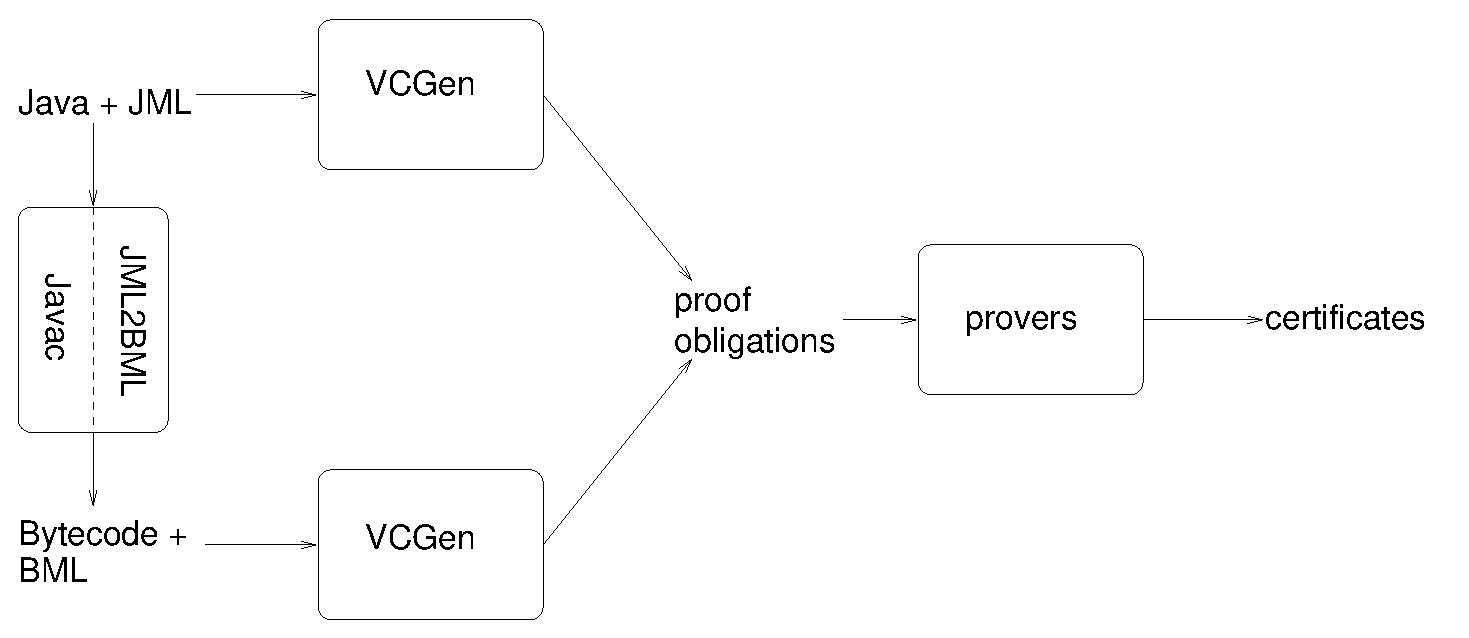
\includegraphics[width=\textwidth]{toolset.eps} 
\caption{Overview of \mobius tool set}\label{FigToolSet}
\end{figure}
As part of the \mobius project, we plan to develop a tool set that
supports both JML and BML. Figure~\ref{FigToolSet} outlines the
general architecture of this tool set. Thus, both Java/JML and
bytecode/BML can be used as input application. For both specification
languages, verification condition generators are used to generate
appropriate proof obligations that can be discharged with a theorem
prover (either automatic or interactive). To support the proof
carrying code platform, the provers will be instrumented to produce
certificates. In addition, source code applications annotated with JML
can be compiled into bytecode annotated with BML.

The development of the JML subcomponent of the tool set will be based
on experiences with ESC/Java~\cite{CokK04} and JACK~\cite{BurdyRL03}.
Several tools and algorithms (notably the compiler and the
verification condition generator) for BML have already been
implemented, see~\cite{BurdyP06}, but more work is needed to cover the
whole language. Moreover, to make the tool set usable in practice, we
will also need a tool to inspect and write directly BML
specifications, and a run-time checker for BML specifications. The
latter can be implemented by a code transformation, inserting explicit
run-time checks in the bytecode, or by extending the virtual machine
to take the user-specific attributes with specifications into account;

Our initial experiments with compilation of specifications has shown
that there exists indeed a correspondence between the proof
obligations generated at source and at bytecode level, modulo
differences in elimination of trivial goals, handling of arithmetic
expressions, and the naming convention of generated
variables. Moreover, when the proofs are done with the Coq prover,
different names are generated for hypotheses at source code and
bytecode level. It is future work to clean up the compilation, so
there is a one-to-one correspondence.




 

\subsection*{Related work}
The interest in specification and verification of bytecode
applications is quite recent, and not too much work has been done in
that direction. Several logics have been developed to reason about
bytecode, \emph{e.g.}~by Bannwart \& M\"uller~\cite{BannwartMueller05}
and within the MRG project~\cite{AspinallEtAl:TPHOLs2004}. However,
in this work, no attention is given to how one can conveniently write
understandable specifications for bytecode.

The development of BML is clearly inspired by the development of the
JML specification language~\cite{JMLReferenceManual05}. Both JML and
BML follow the Design by Contract principle introduced first in
Eiffel~\cite{Meyer97}. The Boogie project~\cite{BarnettCDJL05}
introduces in similarly the Design by Contract principles into the C\#
programming language, both at source code level and for CIL, the .NET
intermediate language.  The possibility to check a property at
run-time, using the \texttt{assert} construct, has been long 
adopted in the C programming language and recently also in Java (Java
1.5, see \cite[\S 14.10]{JLS}). 

Finally, we should mention the Extended Virtual Platform
project\footnote{See
\url{http://www.cs.usm.maine.edu/~mroyer/xvp/}.}. This project aims at
developing a framework that allows to compile JML annotations, to
allow run-time checking~\cite{AlagicXVP05}. However, in contrast to
our work, they do not intend to do static verification of bytecode
programs. Moreover, their platform takes JML-annotated source code
files as starting point, while with BML one is able to annotate
bytecode applications directly\footnote{Some security-critical
applications are written in bytecode directly, to avoid security
problems related with compilation. Thus, for such applications one
needs to be able to specify and verify them directly at this level.}.



\subsection*{Acknowledgements}
We thank Lennart Beringer and Olha Shkaravska for discussions about
the semantics of BML. 




\bibliographystyle{plain}
\bibliography{bytecode,../specification}

\appendix
% generated and manually adapted from BML-grammar.texinfo

\newdimen{\standardmargin}  \setlength{\standardmargin}{15pt}
\newdimen{\tableindent}     \setlength{\tableindent}{50pt}
\newbox\ItemBox

\setcounter{secnumdepth}{5}       
\setcounter{tocdepth}{5}          

\def\lqHook{\char16 }\def\rqHook{\char17 }\def\lnqHook{\char96 }\def\rnqHook{\char39 }%
%\usepackage{varioref}         




\newcommand{\lbr}{\ifvmode\else\unskip\relax\nobreak\hfil\break\fi}




\newenvironment{display}[1][\standardmargin]%
                       {\begingroup\def~{\mbox{ }}\let\\=\lbr
                        \list{}{\listparindent0pt  \itemindent0pt
                        \rightmargin0pt    \leftmargin#1}%
                \item}
               {\endlist\endgroup}



\renewenvironment{quote}
                 {\list{}{\leftmargin\standardmargin\rightmargin\leftmargin}%
                  \item\relax}
                 {\endlist}



\makeatletter
\newcommand\Nopagebreak{\let\if@nobreak\iftrue \nopagebreak}
\makeatother





\newcommand{\tabletermHook}[1]{#1}

\newcommand{\kbdHook}[1]{\mbox{\ttfamily\slshape #1}}

\newcommand{\keyHook}[1]{{\fboxsep2pt\fbox{\sffamily\footnotesize #1}}}
\newcommand{\sampHook}[1]{\lnqHook\texttt{#1}\rnqHook}
\newcommand{\verbHook}[1]{\mbox{\ttfamily #1}}
\newcommand{\envHook}[1]{\mbox{\ttfamily #1}}
\newcommand{\fileHook}[1]{\lnqHook\texttt{#1}\rnqHook}
\newcommand{\commandHook}[1]{\mbox{\ttfamily #1}}
\newcommand{\optionHook}[1]{\lnqHook\mbox{\ttfamily #1}\rnqHook}
\newcommand{\dfnHook}[1]{\emph{#1}}
\newcommand{\citeHook}[1]{\textit{#1}}
\newcommand{\abbrevwordHook}[1]{#1}
\newcommand{\abbrevdescHook}[1]{ (#1)}
\newcommand{\acronymwordHook}[1]{\mbox{#1}}
\newcommand{\acronymdescHook}[1]{\footnote{#1}}
\newcommand{\urlHook}[1]{#1}
\newcommand{\emailHook}[1]{#1}

\newcommand{\emphHook}[1]{\emph{#1}}
\newcommand{\strongHook}[1]{\textbf{#1}}
\newcommand{\scHook}[1]{\textsc{#1}}
\newcommand{\slantedHook}[1]{\textsl{#1}}
\newcommand{\sansserifHook}[1]{\textsf{#1}}
\newcommand{\iHook}[1]{\textit{#1}}
\newcommand{\bHook}[1]{\textbf{#1}}
\newcommand{\tHook}[1]{\texttt{#1}}
\newcommand{\rHook}[1]{\textrm{#1}}
\newcommand{\dmnHook}[1]{\,\mbox{#1}}
\newcommand{\mathHook}[1]{\ensuremath{#1}}
\newcommand{\footnoteHook}[1]{\footnote{#1}}



\newenvironment{quotationHook}{\begin{quote}}{\end{quote}}
\newenvironment{copyingHook}{\begin{quote}}{\end{quote}}
\newenvironment{verbatimHook}{\begin{display}[0pt]\ttfamily}{\end{display}}
\newenvironment{exampleHook}{\begin{display}\ttfamily}{\end{display}}
\newenvironment{lispHook}{\begin{display}\ttfamily}{\end{display}}
\newenvironment{displayHook}{\begin{display}\relax}{\end{display}}
\newenvironment{formatHook}{\begin{display}[0pt]}{\end{display}}

\newenvironment{smallexampleHook}{\begin{small}\begin{exampleHook}}%
    {\end{exampleHook}\end{small}}
\newenvironment{smalldisplayHook}{\begin{small}\begin{displayHook}}%
    {\end{displayHook}\end{small}}
\newenvironment{smallformatHook}{\begin{small}\begin{formatHook}}%
    {\end{formatHook}\end{small}}
\newenvironment{smalllispHook}{\begin{small}\begin{lispHook}}%
    {\end{lispHook}\end{small}}

\newenvironment{flushleftHook}{\begin{flushleft}}{\end{flushleft}}
\newenvironment{flushrightHook}{\begin{flushright}}{\end{flushright}}
\newenvironment{groupHook}{\begin{samepage}}{\end{samepage}}

\newenvironment{cartoucheHook}{\begin{center}\shadowbox\bgroup
    \hbox to \hsize\bgroup\begin{minipage}{\hsize}}%
    {\end{minipage}\hss\egroup\egroup\end{center}}

\newcommand{\centerHook}[1]{\centerline{#1}}




\newenvironment{definitionitem}[1][\standardmargin]
               {\list{}{\listparindent0pt  \itemindent0pt
                        \rightmargin0pt    \leftmargin#1}%
                \item\removelastskip\relax}
               {\endlist}

\sloppy               
\hbadness20000





%\PassOptionsToPackage{hyphens}{url}
%\newcommand{\xhyphen}{\discretionary{\char127}{}{-}}
%\IfFileExists{pdfcprot.sty}{\usepackage[activate]{pdfcprot}}{}
%\usepackage[%
%  pagebackref=true,pdfstartview=FitH,
%  pdfcreator={texi2latex + LaTeX with hyperref package},
%  pdfpagelayout=OneColumn,
%  bookmarks=true,bookmarksopen=false,  colorlinks,pdfpagelabels=true,
%  draft=false,breaklinks=true,plainpages=false]{hyperref}[2000/05/08]  \hypersetup{%
%    pdftitle={BML grammar},
%    pdfsubject={<setfilename>BML-grammar.texinfo</setfilename>},
%    pdfauthor={}
%  }
%\urlstyle{rm}




%\usepackage{hypbmsec}



%\InputIfFileExists{texi2latex.cfg}%
%  {\message{Loading global configuration file texi2latex.cfg}}{}
%\InputIfFileExists{\jobname-t2l.cfg}%
%  {\message{Loading local configuration file \jobname-t2l.cfg}}{}



%\begin{document}


\gdef\InsertLabelMaybe{\label{predicates-and-specification-expressions}\gdef\InsertLabelMaybe{}}
\section{Grammar for BML predicates and specification expressions}\label{AppBML}\InsertLabelMaybe

\textbf{NOTE: We intend to set up a webpage with the complete BML grammar 
before publication. This grammar is included for the reviewer's
convenience, but will not be included in the final version of the
paper.}

As in the JML Reference Manual~\cite{JMLReferenceManual05}, we use an
extended Backus-Nauer Form (BNF) grammar to describe the syntax of
JML. The extensions are as follows~\cite{Ledgard80}.

\begin{itemize}
\item Nonterminal symbols are written as follows: \varHook{nonterminal}.

\item Terminal symbols are written as follows: \codeHook{terminal}.

\item Square brackets ([ and ]) surround optional text. Notice that
\codeHook{[} and \codeHook{]} are terminal symbols.  

\item The notation \dots\ means that the preceding nonterminal or group of optional text can be repeated zero or more times.  
\end{itemize}

\begin{displayHook}\\\relax {\varHook{predicate}}~::=~{\varHook{spec-{}expression}}\\\relax {\varHook{spec-{}expression-{}list}}~::=~{\varHook{spec-{}expression}}\\\relax ~~~~~~~~~~~~~~~~~~~~~~~~~[~{\codeHook{,}}~{\varHook{spec-{}expression}}~]~\dots \@{}\\\relax {\varHook{spec-{}expression}}~::=~{\varHook{expression}}\\\relax {\varHook{expression-{}list}}~::=~{\varHook{expression}}~[~{\codeHook{,}}~{\varHook{expression}}~]~\dots \@{}\\\relax {\varHook{expression}}~::=~{\varHook{conditional-{}expr}}~\\\relax {\varHook{conditional-{}expr}}~::=~{\varHook{equivalence-{}expr}}\\\relax ~~~~~~~~~~~~~~~~~~~[~{\codeHook{?{}}}~{\varHook{conditional-{}expr}}~{\codeHook{:}}~{\varHook{conditional-{}expr}}~]\\\relax {\varHook{equivalence-{}expr}}~::=~{\varHook{implies-{}expr}}\\\relax ~~~~~~~~~~~~~~~~~~~~~[~{\varHook{equivalence-{}op}}~{\varHook{implies-{}expr}}~]~\dots \@{}\\\relax {\varHook{equivalence-{}op}}~::=~{\codeHook{<{}==>{}}}~{\mbox{\char124{}}}~{\codeHook{<{}=!{}=>{}}}\\\relax {\varHook{implies-{}expr}}~::=~{\varHook{logical-{}or-{}expr}}\\\relax ~~~~~~~~~~~~~[~{\codeHook{==>{}}}~{\varHook{implies-{}non-{}backward-{}expr}}~]\\\relax ~~~~~~~~{\mbox{\char124{}}}~{\varHook{logical-{}or-{}expr}}~{\codeHook{<{}==}}~{\varHook{logical-{}or-{}expr}}\\\relax ~~~~~~~~~~~~~[~{\codeHook{<{}==}}~{\varHook{logical-{}or-{}expr}}~]~\dots \@{}\\\relax {\varHook{implies-{}non-{}backward-{}expr}}~::=~{\varHook{logical-{}or-{}expr}}\\\relax ~~~~~~~~~~~~~[~{\codeHook{==>{}}}~{\varHook{implies-{}non-{}backward-{}expr}}~]\\\relax {\varHook{logical-{}or-{}expr}}~::=~{\varHook{logical-{}and-{}expr}}~[~`{}{\codeHook{{\mbox{\char124{}}}{\mbox{\char124{}}}}}'{}~{\varHook{logical-{}and-{}expr}}~]~\dots \@{}\\\relax {\varHook{logical-{}and-{}expr}}~::=~{\varHook{inclusive-{}or-{}expr}}~[~{\codeHook{\&\&}}~{\varHook{inclusive-{}or-{}expr}}~]~\dots \@{}\\\relax {\varHook{inclusive-{}or-{}expr}}~::=~{\varHook{exclusive-{}or-{}expr}}~[~`{}{\codeHook{{\mbox{\char124{}}}}}'{}~{\varHook{exclusive-{}or-{}expr}}~]~\dots \@{}\\\relax {\varHook{exclusive-{}or-{}expr}}~::=~{\varHook{and-{}expr}}~[~{\codeHook{{\mbox{\char94{}}}}}~{\varHook{and-{}expr}}~]~\dots \@{}\\\relax {\varHook{and-{}expr}}~::=~{\varHook{equality-{}expr}}~[~{\codeHook{\&}}~{\varHook{equality-{}expr}}~]~\dots \@{}\\\relax {\varHook{equality-{}expr}}~::=~{\varHook{relational-{}expr}}~[~{\codeHook{==}}~{\varHook{relational-{}expr}}]~\dots \@{}\\\relax ~~~~~~~~{\mbox{\char124{}}}~{\varHook{relational-{}expr}}~[~{\codeHook{!{}=}}~{\varHook{relational-{}expr}}]~\dots \@{}\\\relax {\varHook{relational-{}expr}}~::=~{\varHook{shift-{}expr}}~{\codeHook{<{}}}~{\varHook{shift-{}expr}}\\\relax ~~~~~~~~{\mbox{\char124{}}}~{\varHook{shift-{}expr}}~{\codeHook{>{}}}~{\varHook{shift-{}expr}}\\\relax ~~~~~~~~{\mbox{\char124{}}}~{\varHook{shift-{}expr}}~{\codeHook{<{}=}}~{\varHook{shift-{}expr}}\\\relax ~~~~~~~~{\mbox{\char124{}}}~{\varHook{shift-{}expr}}~{\codeHook{>{}=}}~{\varHook{shift-{}expr}}\\\relax ~~~~~~~~{\mbox{\char124{}}}~{\varHook{shift-{}expr}}~{\codeHook{<{}:}}~{\varHook{shift-{}expr}}\\\relax ~~~~~~~~{\mbox{\char124{}}}~{\varHook{shift-{}expr}}~[~{\codeHook{instanceof}}~{\varHook{type-{}spec}}~]\\\relax {\varHook{shift-{}expr}}~::=~{\varHook{additive-{}expr}}~[~{\varHook{shift-{}op}}~{\varHook{additive-{}expr}}~]~\dots \@{}\\\relax {\varHook{shift-{}op}}~::=~{\codeHook{<{}<{}}}~{\mbox{\char124{}}}~{\codeHook{>{}>{}}}~{\mbox{\char124{}}}~{\codeHook{>{}>{}>{}}}\\\relax {\varHook{additive-{}expr}}~::=~{\varHook{mult-{}expr}}~[~{\varHook{additive-{}op}}~{\varHook{mult-{}expr}}~]~\dots \@{}\\\relax {\varHook{additive-{}op}}~::=~{\codeHook{+}}~{\mbox{\char124{}}}~{\codeHook{-{}}}\\\relax {\varHook{mult-{}expr}}~::=~{\varHook{unary-{}expr}}~[~{\varHook{mult-{}op}}~{\varHook{unary-{}expr}}~]~\dots \@{}\\\relax {\varHook{mult-{}op}}~::=~{\codeHook{*}}~{\mbox{\char124{}}}~{\codeHook{/}}~{\mbox{\char124{}}}~{\codeHook{\%}}\\\relax {\varHook{unary-{}expr}}~::=~{\codeHook{(}}~{\varHook{type-{}spec}}~{\codeHook{)}}~{\varHook{unary-{}expr}}\\\relax ~~~~~~~~{\mbox{\char124{}}}~{\codeHook{+}}~{\varHook{unary-{}expr}}\\\relax ~~~~~~~~{\mbox{\char124{}}}~{\codeHook{-{}}}~{\varHook{unary-{}expr}}\\\relax ~~~~~~~~{\mbox{\char124{}}}~{\varHook{unary-{}expr-{}not-{}plus-{}minus}}\\\relax {\varHook{unary-{}expr-{}not-{}plus-{}minus}}~::=~{\codeHook{{\mbox{\char126{}}}}}~{\varHook{unary-{}expr}}\\\relax ~~~~~~~~{\mbox{\char124{}}}~{\codeHook{!{}}}~{\varHook{unary-{}expr}}\\\relax ~~~~~~~~{\mbox{\char124{}}}~{\codeHook{(}}~{\varHook{built-{}in-{}type}}~{\codeHook{)}}~{\varHook{unary-{}expr}}\\\relax ~~~~~~~~{\mbox{\char124{}}}~{\codeHook{(}}~{\varHook{reference-{}type}}~{\codeHook{)}}~{\varHook{unary-{}expr-{}not-{}plus-{}minus}}\\\relax ~~~~~~~~{\mbox{\char124{}}}~{\varHook{primary-{}expr}}~[~{\varHook{primary-{}suffix}}~]~\dots \@{}\\\relax {\varHook{primary-{}suffix}}~::=~{\codeHook{(}}~[~{\varHook{expression-{}list}}~]~{\codeHook{)}}\\\relax ~~~~~~~~{\mbox{\char124{}}}~`{}{\codeHook{[}}'{}~{\varHook{expression}}~`{}{\codeHook{]}}'{}\\\relax {\varHook{primary-{}expr}}~::=~~{\codeHook{{\mbox{\char92{}}}{\mbox{\char35{}}}}}{\varHook{natural}}~{\mbox{\char124{}}}~{\codeHook{lv[}}~{\varHook{natural}}~{\codeHook{]}}\\\relax ~~~~~~~~{\mbox{\char124{}}}~{\varHook{constant}}~{\mbox{\char124{}}}~{\codeHook{super}}~{\mbox{\char124{}}}~{\codeHook{true}}\\\relax ~~~~~~~~{\mbox{\char124{}}}~{\codeHook{false}}~{\mbox{\char124{}}}~{\codeHook{this}}~{\mbox{\char124{}}}~{\codeHook{null}}\\\relax ~~~~~~~~{\mbox{\char124{}}}~{\codeHook{(}}~{\varHook{expression}}~{\codeHook{)}}\\\relax ~~~~~~~~{\mbox{\char124{}}}~{\varHook{bml-{}primary}}\\\relax ~~~~~~~~{\mbox{\char124{}}}~{\varHook{jml-{}primary}}\\\relax {\varHook{built-{}in-{}type}}~::=~{\codeHook{void}}~{\mbox{\char124{}}}~{\codeHook{boolean}}~{\mbox{\char124{}}}~{\codeHook{byte}}\\\relax ~~~~~~~~{\mbox{\char124{}}}~{\codeHook{char}}~{\mbox{\char124{}}}~{\codeHook{short}}~{\mbox{\char124{}}}~{\codeHook{int}}\\\relax ~~~~~~~~{\mbox{\char124{}}}~{\codeHook{long}}~{\mbox{\char124{}}}~{\codeHook{float}}~{\mbox{\char124{}}}~{\codeHook{double}}\\\relax {\varHook{constant}}~::=~{\varHook{java-{}literal}}\\\relax {\varHook{bml-{}primary}}~::=~{\varHook{array-{}length-{}expression}}~{\mbox{\char124{}}}\\\relax ~~~~~~~~~~~{\mbox{\char124{}}}~{\varHook{opstack-{}counter-{}expression}}\\\relax ~~~~~~~~~~~{\mbox{\char124{}}}~{\varHook{stack-{}expresion}}\\\relax {\varHook{array-{}length-{}expression}}~::=~{\codeHook{length(}}~{\varHook{expression}}~{\codeHook{)}}\\\relax {\varHook{opstack-{}counter-{}expression}}~::=~{\codeHook{cntr}}\\\relax {\varHook{stack-{}expression}}~::=~{\codeHook{st(}}~{\varHook{additive-{}expr}}~{\codeHook{)}}\\\relax {\varHook{jml-{}primary}}~::=~{\varHook{result-{}expression}}\\\relax ~~~~~~~~{\mbox{\char124{}}}~{\varHook{old-{}expression}}\\\relax ~~~~~~~~{\mbox{\char124{}}}~{\varHook{fresh-{}expression}}\\\relax ~~~~~~~~{\mbox{\char124{}}}~{\varHook{nonnullelements-{}expression}}\\\relax ~~~~~~~~{\mbox{\char124{}}}~{\varHook{typeof-{}expression}}\\\relax ~~~~~~~~{\mbox{\char124{}}}~{\varHook{elemtype-{}expression}}\\\relax ~~~~~~~~{\mbox{\char124{}}}~{\varHook{type-{}expression}}\\\relax ~~~~~~~~{\mbox{\char124{}}}~{\varHook{spec-{}quantified-{}expr}}\\\relax {\varHook{result-{}expression}}~::=~{\codeHook{{\mbox{\char92{}}}result}}\\\relax {\varHook{old-{}expression}}~::=~{\codeHook{{\mbox{\char92{}}}old}}~{\codeHook{(}}~{\varHook{spec-{}expression}}~{\codeHook{)}}\\\relax ~~~~~~~~{\mbox{\char124{}}}~{\codeHook{{\mbox{\char92{}}}pre}}~{\codeHook{(}}~{\varHook{spec-{}expression}}~{\codeHook{)}}\\\relax {\varHook{fresh-{}expression}}~::=~{\codeHook{{\mbox{\char92{}}}fresh}}~{\codeHook{(}}~{\varHook{spec-{}expression-{}list}}~{\codeHook{)}}\\\relax {\varHook{nonnullelements-{}expression}}~::=~{\codeHook{{\mbox{\char92{}}}nonnullelements}}~{\codeHook{(}}~{\varHook{spec-{}expression}}~{\codeHook{)}}\\\relax {\varHook{typeof-{}expression}}~::=~{\codeHook{{\mbox{\char92{}}}typeof}}~{\codeHook{(}}~{\varHook{spec-{}expression}}~{\codeHook{)}}\\\relax {\varHook{elemtype-{}expression}}~::=~{\codeHook{{\mbox{\char92{}}}elemtype}}~{\codeHook{(}}~{\varHook{spec-{}expression}}~{\codeHook{)}}\\\relax {\varHook{type-{}expression}}~::=~{\codeHook{{\mbox{\char92{}}}type}}~{\codeHook{(}}~{\varHook{type}}~{\codeHook{)}}\\\relax {\varHook{spec-{}quantified-{}expr}}~::=~{\codeHook{(}}~{\varHook{quantifier}}~{\varHook{quantified-{}var-{}decls}}~{\codeHook{;}}\\\relax ~~~~~~~~~~~~~~~~~~~~~~~~~~~[~[~{\varHook{predicate}}~]~{\codeHook{;}}~]\\\relax ~~~~~~~~~~~~~~~~~~~~~~~~~~~{\varHook{spec-{}expression}}~{\codeHook{)}}\\\relax {\varHook{quantifier}}~::=~{\codeHook{{\mbox{\char92{}}}forall}}~{\mbox{\char124{}}}~{\codeHook{{\mbox{\char92{}}}exists}}\\\relax {\varHook{quantified-{}var-{}decls}}~::=~[~{\varHook{bound-{}var-{}modifiers}}~]~{\varHook{type-{}spec}}~{\varHook{quantified-{}var-{}declarator}}\\\relax ~~~~~~~~~~~~~~~~~~~~~~~~~[~{\codeHook{,}}~{\varHook{quantified-{}var-{}declarator}}~]~\dots \@{}\\\relax {\varHook{quantified-{}var-{}declarator}}~::=~{\varHook{ident}}~[~{\varHook{dims}}~]\\\relax {\varHook{bound-{}var-{}modifiers}}~::=~{\codeHook{non{\mbox{\char95{}}}null}}~{\mbox{\char124{}}}~{\codeHook{nullable}}\\\relax {\varHook{store-{}ref-{}list}}~::=~{\varHook{store-{}ref}}~[~{\codeHook{,}}~{\varHook{store-{}ref}}~]~\dots \@{}\\\relax {\varHook{store-{}ref}}~::=~{\varHook{store-{}ref-{}expression}}\\\relax ~~~~~~~~{\mbox{\char124{}}}~{\varHook{store-{}ref-{}keyword}}\\\relax {\varHook{store-{}ref-{}expression}}~::=~{\varHook{store-{}ref-{}name}}~[~{\varHook{store-{}ref-{}name-{}suffix}}~]~\dots \@{}\\\relax {\varHook{store-{}ref-{}name}}~::=~{\codeHook{{\mbox{\char92{}}}{\mbox{\char35{}}}}}~{\varHook{natural}}~{\mbox{\char124{}}}~{\codeHook{super}}~{\mbox{\char124{}}}~{\codeHook{this}}\\\relax {\varHook{store-{}ref-{}name-{}suffix}}~::=~{\codeHook{(}}~{\varHook{store-{}ref-{}expression}}~{\codeHook{)}}\\\relax ~~~~~~~~{\mbox{\char124{}}}~`{}{\codeHook{[}}'{}~{\varHook{spec-{}array-{}ref-{}expr}}~`{}{\codeHook{]}}'{}\\\relax {\varHook{spec-{}array-{}ref-{}expr}}~::=~{\varHook{spec-{}expression}}\\\relax ~~~~~~~~{\mbox{\char124{}}}~{\varHook{spec-{}expression}}~{\codeHook{..}}~{\varHook{spec-{}expression}}\\\relax ~~~~~~~~{\mbox{\char124{}}}~{\codeHook{*}}\\\relax {\varHook{store-{}ref-{}keyword}}~::=~{\codeHook{{\mbox{\char92{}}}nothing}}~{\mbox{\char124{}}}~{\codeHook{{\mbox{\char92{}}}everything}}~{\mbox{\char124{}}}~{\codeHook{{\mbox{\char92{}}}not{\mbox{\char95{}}}specified}}\end{displayHook}


\end{document}

  
\newcommand{\getType}{\mbox{\rm\textsf{getType}}}
\newcommand{\constType}{\mbox{\rm\textsf{constType}}}
\newcommand{\getClass}{\mbox{\rm\textsf{getClass}}}
\newcommand{\application}{\mbox{\rm\textbf{CLS}}}
 
\section{Well formed BML specification}
In the previous Section \ref{BCSLgrammar}, we gave the formal grammar of BML.
However, we are interested in a strict subset of 
the specifications that can be generated from this grammar. In particular, we want that a
BML specification is well typed and respects structural constraints.
The constraints that we impose here are similar to the type and structural constraints
that the bytecode verifier imposes over the class file format.

Examples for type constraints that  a valid BML specification must respect : 
\begin{itemize}
    \item  the array expression $\arrayAccess{\expression^1}{\expression^2}$ must be such that 
$\expression^1$ is of array type and $\expression^2$  is of integer type.

    \item the field access expression  $\fieldAccess{\expression}{\ident}$ is such that $\expression$ is of subtype
    of the class where the field described by the constant pool element at index $\ident$ is declared
    \item For any expression $ \expression^1 \op \expression^2$,  $ \expression^1$ and $ \expression^2$ must be of
          a numeric type.
    
    \item in the predicate $\expression^1 r \expression^2$ where $r =  \leq,<,\geq, >$  the expressions  $\expression^1$ and 
          $\expression^2$ must be of numerical type.

     \item  in the predicate $\expression^1  \subtypeSpec \expression^2$, the expressions $\expression^1$
            and  $\expression^2$ must be of type \TYPE (which is the same as \texttt{java.lang.Class}).

     \item the expression $\elemtype{\expression}$ must be such that $\expression$ has an array type.
	    
     \item  etc.  	   

	  
 \end{itemize}

Example for structural constraint are :
\begin{itemize}
    \item All references to the constant pool must be to an entry of the appropriate type. For example:
          the field access expression  $\fieldAccess{\expression}{\ident}$ is such that the
	  $\ident$ must reference a field in the constant pool; or for the expression $\type{\ident}$, \ident
	  must be a reference to a constant class in the constant pool
    
    \item every $\ident$ in a BML specification must be a correct index in the constant pool table. 
    
    \item if the  expression $\locVar{i}$ appears in a method BML specification, then
          $i$ must be a valid index in the array of local variables of the method
\end{itemize}

An extension of the bytecode verifier may perform the checks
 if a BML specification  respects this kind of structural and type constraints.
However, we have not worked on this problem and is a good candidate for a future work.
For the curious reader, it will be certainly of interest to turn to the Java Virtual Machine 
specification \cite{VMSpec} which contains the official
 specification of the Java bytecode verifier    
or to the existing literature on bytecode verification (see the overview article ~\cite{Ljbc} )
 








  


\section{Compiling JML into BML}\label{BCSLcompile}

%This section explains how JML specifications are compiled into bytecode level specifications and how they are inserted into the bytecode. 

In this section, we turn to the \JMLtoBML \ compiler.
As we shall see, the compilation consists of several phases, namely compiling the Java source file, 
preprocessing of the JML specification, resolution
and linking of names, locating the position of intra --- method specification, processing of boolean expressions and 
finally encoding the BML specification in user defined class file attributes.  (their structure is predefined by JVMS).
In the following, we look in details at the phases of the compilation process:
\begin{enumerate}
\item Compilation of the Java source file \\
  This can be done by any Java compiler that supplies for every method in the generated class file 
  the \textbf{Line\_Number\_Table} \\ 
  and \textbf{Local\_Variable\_Table}  attributes. 
  % The presence in the Java class file format of 
  % these attribute is optional \cite{VMSpec}, yet almost all standard non optimizing compilers can generate these data. 
 %  The \textbf{Line\_Number\_Table} describes the link between the source line and the bytecode of a method.  
 %  The \textbf{Local\_Variable\_Table} describes the local variables that appear in a method. 
   Those attributes are important for the next phases of the JML compilation.

\item Compilation of Ghost field declarations \\
      JML specification is invisible by the 
      Java compilers. Thus Java compilers omit the compilation of ghost variables declaration.
      That is why it is the responsibility of the \JMLtoBML \  compiler to do this work. 
      For instance, the compilation of the declaration of the ghost variable from
      Fig. \ref{bml:ghost} is given in Fig.\ref{bml:compiler:ghost} which shows the data structure \textbf{Ghost\_field\_Attribute}
      in which the information about the field
      \texttt{TRANS} is encoded in the class file format. 
      Note that,  the constant pool indexes \textbf{\#18} and \textbf{\#19}  which contain its description were not in the constant
      pool table of the class file \texttt{Transaction.class} before running the \JMLtoBML \ compiler on it. 
\begin{figure}[ht!]
\begin{frameit}
\textbf{     
\begin{tabbing}
 Gho\=st\_field\_Attribute \{\\
\> ...\\
\> \{\hspace{3 mm}\= access\_flag 10;\\
\> \> name\_ index = \#18; \\
\> \> descriptor\_index = \#19 \\
\> \} ghost[1];\\
\}
\end{tabbing}
}

\begin{itemize}
\item \textbf{access\_flag}: The kind of access that is allowed to the field

\item \textbf{name\_index}:  The index in the constant pool which contains information about the source name of the field

\item \textbf{descriptor\_index}: The index in the constant pool which contains information about the name of the field type  
\end{itemize}


\caption{\sc Compilation of ghost variable declaration}
\label{bml:compiler:ghost}
\end{frameit}
\end{figure}

\item Desugaring of the JML specification \\
      %BML supports less specification clauses than JML for the sake of keeping compact the class file format.
     % In particular BML does not support heavy weight behaviour specification clauses or nested specification, neither an incomplete
     % method specification(see  \cite{JMLRefMan}).
      % Thus, a step in the compilation of JML specification into BML specification is the desugaring of the JML heavy weight
      The phase consists in converting the JML method heavy-weight behaviors and the light - weight non complete
      specification into BML specification cases.
      It corresponds to part of the standard JML desugaring as described  in \cite{RT03djml}.
      For instance, the BML compiler will produce from the specification in Fig.\ref{bml:heavySp} the BML specification 
      given in Fig.\ref{bml:heavySpBML} 
      



\item Linking with source data structures \\
      When the JML specification is desugared, we are ready for the linking and resolving phases.
      In this stage, the JML specification gets into an intermediate format in which 
      the identifiers are resolved to their corresponding data structures in the class file.
      The Java and JML source identifiers are linked with their identifiers on bytecode level, 
      namely with the corresponding indexes either from the constant pool or the array of 
      local variables described in the \textbf{Local\_Variable\_Table} attribute. 

      For instance, consider once again the example in Fig. \ref{bml:heavySp} and more particularly  the first specification
      case of method \texttt{divide}  whose precondition \texttt{ b > 0 }  contains the method parameter identifier \texttt{b}.
      In the linking phase, the identifier \texttt{b} is resolved to the local variable $\locVar{1}$  in the array of
      local variables for the method \texttt{divide}.
      We have a similar situation with the postcondition \texttt{ a == \old{a} / b }  which mentions also the field \texttt{a} of the current object.
      The field name \texttt{a} is compiled to the index in the class constant pool  which describes the constant field reference.
      The result of the linking process is in Fig.\ref{bml:heavySpBML}.

      % how ghost fields are compiled
      If, in the JML specification a field
      identifier appears for which no constant pool index exists, it is added in the constant pool and the identifier in question
      is compiled to the new constant pool index. This happens when declarations of JML ghost fields are compiled. 
     

  





      

\item Locating the points for the intra ---method specification \\

      In this phase the specification parts like the loop invariants and the assertions
      which should hold at a certain point in the source program must be associated to the
      respective program point in the bytecode. For this, the 
      \textbf{Line\_Number\_Table} attribute is used. The \textbf{Line\_Number\_Table} attribute
      describes the correspondence between the Java source line and the instructions of its respective bytecode.
      In particular, for every line in the Java source code the   \textbf{Line\_Number\_Table}  specifies the index 
      of the beginning of the basic block\footnote{a basic block is a sequence of instructions which does not contain jumps except
	may be for the last instruction and neither contains target of jumps except for the first instruction. 
	This notion comes from the compiler community and 
	more information on this one can find at \cite{ARUCom1986}} in the bytecode which corresponds to the source line. 
      Note however, that a source line may correspond to more than one instruction in the \textbf{Line\_Number\_Table}. 
     
      This poses problems for  identifying loop entry instruction of a loop in the bytecode
      which corresponds to a particular loop in the source  code. % which is important for the
     % compilation of the JML loop invariants (as we should know exactly where they must hold in the bytecode). 
       For instance, for method \texttt{replace} in
      the Java source example in Fig. \ref{replaceSrc} the java compiler will  produce two lines in the 
       \textbf{Line\_Number\_Table} which correspond to the source line \textbf{17}  as shown in Fig. \ref{bml:compiler:loopEntry}.
       The problem is that none of the basic blocks determined by instructions  \textbf{2} and  \textbf{18} contain the loop entry instruction of the compilation
       of the loop at line \textbf{17} in Fig. \ref{replaceSrc}. Actually, the loop entry instruction in the bytecode in 
       Fig. \ref{bml:loopBML} (remember that this is the compilation in bytecode of the Java source in Fig. \ref{replaceSrc}) which corresponds to the 
       in the bytecode is at index \textbf{19}.
  
       Thus for identifying  loop entry instruction   corresponding to a particular loop in the source code, we use an heuristics.  
       It consists in looking for the first bytecode loop entry instruction starting from one of the \textbf{start\_pc} indexes 
       (if there is more than one) corresponding to the start
       line of the source loop in the \textbf{Line\_Number\_Table}. 
       The algorithm works under the assumption that the control flow graph of the method bytecode is reducible.
       This assumption  guarantees that the first loop entry instruction found starting the search 
       from  an index in the  \textbf{Line\_Number\_Table} corresponding to the first line of a source loop
       will be the loop entry corresponding to this source loop.
       However, we do not have a formal argumentation for this algorithm because it depends on the particular implementation of the compiler.
       From our experiments, the heuristic works successfully for the Java Sun non optimizing compiler.
 
\begin{figure}[t]
\begin{frameit}
\textbf{Line\_Number\_Table} 
\textbf{     
\begin{tabbing}
start\_pc \= line \\
\ldots \> \\
2 \> 17 \\
18  \> 17 \\
\end{tabbing}
}

\caption{\textbf{Line\_Number\_Table}  {\sc for the method } \texttt{replace} {\sc in Fig.  \ref{replaceSrc}  } }
\label{bml:compiler:loopEntry}
\end{frameit}
\end{figure} \todo{une presentation tres laide }

      
      
\item Compilation of the JML boolean expressions into BML \\
      
     

Another important issue in this stage of the JML compilation is how the type differences on source and bytecode level are treated. 
By type differences we refer to the fact that the JVM (Java Virtual Machine) does not provide direct support for integral types 
like byte, short, char, neither for boolean. Those types are rather encoded as integers in the bytecode. Concretely, this means that 
if a Java source variable has a boolean type it will be compiled to a variable with
an integer type.


 For instance, in the example for the method 
\texttt{replace} and its specification in Fig.\ref{replaceSrc} the postcondition states the equality between the JML expression  
\result \ and a predicate. This is correct as the method \texttt{replace} in the Java source is declared with return type boolean  and thus,
 the expression \result \ has type boolean. 
Still, the bytecode resulting from the compilation of the method  \texttt{replace} returns a value of type integer. This means that the JML compiler has to 
``make more effort'' than simply compiling the left and right side of the equality in the postcondition, otherwise its compilation will not make sense as 
it will not be well typed. Actually, if the JML specification contains program boolean expressions that the Java compiler will compile to bytecode expression
 with an integer type, the JML compiler will also compile them in integer expressions and will transform the specification condition in equivalent 
one\footnote{when generating proof obligations we add for every source boolean expression an assumption that it
 must be equal to 0 or 1. A reasonable compiler would encode boolean values in a similar way}.  

Finally, the compilation of the postcondition of method \texttt{replace} is given in Fig. \ref{postCompile}. From the postcondition compilation,
 one can see that the expression \result \ has integer type and the equality between the boolean expressions in the postcondition in Fig.\ref{replaceSrc} is
 compiled into logical equivalence. 
% The example also 
% shows that local variables and  fields are respectively linked to the index of the register table for the method and to the corresponding 
% index of the constant pool table 
% (\#19 is the compilation of the field name \texttt{list} and $\locVar{1}$ stands for the method parameter \texttt{obj}). 

\begin{figure}[t]
\begin{frameit}
 $$\begin{array}{l}
         \result = 1 \\
          \\ 
         \iff \\ 
         \exists    \bound\_{\mbox{\rm \textsf{0}}}, 
           \biggl(\begin{array}{l} \ 0 \leq  \bound\_{\mbox{\rm \textsf{0}}} \wedge\\ 
             \bound\_{\mbox{\rm \textsf{0}}} < len(\#19(\locVar{0})) \wedge \\
             \arrayAccess{\#19(\locVar{0})}{\bound\_{\mbox{\rm \textsf{0}}} } = \locVar{1} 
         \end{array} \biggr) 
   \end{array}
$$
\caption{\sc The compilation of the postcondition in Fig. \ref{replaceSrc}}
\label{postCompile}
\end{frameit}
\end{figure}





\item Encoding BML specification  into user defined class attributes\\
  The specification expression and predicates
  are compiled in binary form using tags in the standard way. The compilation of an expression is a tag followed by the compilation of its subexpressions. 
    
 Method specifications, class invariants, loop invariants are newly defined attributes in the class file.
 For example, the specifications of all the loops in a method are compiled to a unique method attribute whose syntax is
 given in Fig.~\ref{loopAttribute}. This attribute is an array of data structures each describing a single loop from the method source code.
From the figure, we notice that every element describing the specification for a particular loop contains the index of the corresponding loop
entry instruction \textbf{index}, the loop modifies clause (\textbf{modifies}),
the loop invariant (\textbf{invariant}), an expression which guarantees termination (\textbf{decreases}).


\end{enumerate}

\begin{figure}[t]
\begin{frameit}
\textbf{     
\begin{tabbing}
JML\=Loop\_specification\_attribute \{\\
\> ...\\
\> \{\hspace{3 mm}\= u2 index;\\
\> \> u2 modifies\_count;\\
\> \> formula modifies[modifies\_count];\\
\> \> formula invariant;\\
\> \> expression decreases;\\
\> \} loop[loop\_count];\\
\}
\end{tabbing}
}

\begin{itemize}
\item \textbf{index}: The index in the  \texttt{LineNumberTable } where the beginning of the corresponding loop is described

\item \textbf{modifies[]}: The array of locations that may be modified

\item \textbf{invariant }: The predicate that is the loop invariant. It is a compilation of the JML formula in the low level specification language

\item \textbf{decreases}: The expression which decreases at every loop iteration
\end{itemize}
\caption{\sc Structure of the Loop Attribute}
\label{loopAttribute}
\end{frameit}
\end{figure}

% The JML compiler does not depend on any specific Java compiler, but it requires the presence of a debugging information,
%namely the presence of the \textbf{Line\_Number\_Table} attribute for the correct compilation of inter method
% specification, i.e. loops and assertions. We think that this is an acceptable restriction as few bytecode programs even handwritten are not reducible.
% The most problematic part of the compilation is to identify which source loop corresponds to which bytecode loop in the control flow
% graph.
%  To do this, we assume that the control flow graph is reducible (see~\cite{ARUCom1986}), i.e. there are no
% jumps from outside a loop inside it; graph reducibility allows to establish the same order between loops in the
% bytecode and source code level and to compile the invariants to the correct places in the bytecode.
% \todo{put it elsewhere}

%\todo{limitations : registers that are used with two different types in the method bytecode}



\chapter{Assertion language for the verification condition generator}\label{assertLang}
  %\section{Assertion language for the verification condition generator}\label{bml:assertionLang}
% why do we concentrate only on a particular part of BML
In this chapter we shall focus on 
 a particular fragment of BML which will be extended with 
few new constructs.  The part of BML in question  
is the assertion language that our  verification condition generator manipulates
 as we shall see in the next Chapter \ref{wpGeneral}.

% what is exactly the fragment of interest
% The BML fragment that will be of interest here will be the language of BML expressions
% (nonterminal $\expression$) and the  language of the BML predicates (nonterminal $\formulaBc$). 
% % why do we discard the rest. 
% We abstract from the rest of the BML grammar, as it boils down to BML
% expressions and  predicates. We will discuss what is the encoding of the method
% specification which is used by the verification condition generator.


The assertion language presented here will abstract from most of the BML specification clauses described in Section \ref{BCSLgrammar}.
Our interest will be focused only on method and loop specification.
Note that  the assertion language presented here discards class invariants,
 history constraints  because  they boil down to method pre and postconditions. 
%Specification inheritance in case of overriden methods also can be encoded as method pre and postconditions.  


The rest of this chapter is organized as follows. Section \ref{assertLang:lang} presents
what is exactly the BML fragment of interest and its extensions.
Section \ref{methExtend} shows how we encode method and loop specification as well as presents a discussion
how some of the ignored BML specification constructs are transformed into method pre and postconditions.
The last two sections are concentrated on the formal meaning of the assertion language, i.e.
Section \ref{subst} defines the substitution for the assertion language and 
 Section \ref{interpret} gives formal semantics of the assertion language.


  \section{The assertion language} \label{assertLang:lang}
The assertion language in which we are interested corresponds to the
BML  expressions (nonterminal $\expression$) and predicates 
(nonterminal $\formulaBc$) extended with several new constructs.
 The extensions that we add are the following:
\begin{itemize}
    \item Extensions to expressions. 
         The assertion language that we present here must be suitable for the verification condition calculus.
	 Because the verification calculus talks about updated field and array access
	 we should be able  to express  them in the assertion language. Thus we extend the grammar of BML expression
	 with the following constructs concerning update of fields and arrays :

        \begin{itemize}
	       \item update field access expression 
		  $\update{\fieldd}{ \expression}{\expression}(\expression)$.

	       \item update array access expression \\
                   $ \update{ \arrayAccessOnly}{ (\expression , \expression)}{ \expression} (\expression,\expression)$
	\end{itemize}

	The verification calculus will need to talk about reference values. Thus we extend the BML expression grammar to  support
	reference values \RefValues. Note that in the following integers \Myint\  and \RefValues \ will be referred to with \Values.
    \item Extensions to predicates. Our bytecode language is object oriented and thus supports new object creation. Thus we
          will need a means for expressing that a new object has been created during the method execution. 

	  We extend the language of BML  formulas
	  with a new user defined predicate $ \instances(\RefValues)$. Informally, the semantics of the predicate \\
	  $\instances(\referenceOnly)$ where $\referenceOnly \in \RefValues$
	  means that the reference $\referenceOnly  $  has been allocated when the current method started execution.
        
\end{itemize}

The assertion language will use the names of fields and classes for the sake of readability instead of their corresponding indexes
in the constant pool as is in BML.

We would like to discuss in the following how and why BML constructs like class invariants and history constraints can be expressed as 
method pre and postconditions:

\begin{itemize}
  \item Class invariants. A class invariant (\ClassInv)  is a property that must hold at every visible state of the class. This means that a
        class invariant must hold when a method is called and also must be established at the end of a method execution. 
	A class invariant must be established in the poststate 
	of the constructor of this class.
	Thus the semantics of
	a class invariant is part of the pre and  postcondition of every method and is a part of the postcondition of the constructor of the class.
  \item History constraints. A class history constraint (\ClassHistoryConstr) gives a relation between the pre and poststate of every method in the class. 
        A class history constraint thus can be expressed as a postcondition of every method in the class.
        
\end{itemize}

 % why do we discard the rest. 
% We abstract from the rest of the BML grammar, as it boils down to BML
% expressions and  predicates. 



  \section{Substitution} \label{subst}
In this section we focus on how substitution is defined in our assertion language. Basically, it is is defined inductively 
in a standard way over the expression structure. Still, we
extend substitution to deal with field and array update as follows:

$$ \substitution{\expression}{ \fieldd }{ \update{\fieldd}{\expression}{\expression} } $$
This substitution does not affect any of the ground expressions,, i.e. it does not affect 
local variables ($\locVar{i}$), the constants of our language (\ConstantsWp),  the stack counter (\counter), the result expression
(\result), the thrown exception instance variable (\EXC). For instance, the following substitution does not change $\locVar{1}$: 
$$
 \substitution{\locVar{1}}{ \fieldd }{ \update{\fieldd}{\expression}{\expression} } = \locVar{1}
$$   

Field substitution affects only field objects as we see in the following: 



 
 %This is done by establishing the substitution rule for field access as follows:
 %$$  \substitution{\fieldd ( \expression^1)}{ \expression^2}{ \expression^3} =
 %\substitution{\fieldd}{ \expression^2}{ \expression^3} (  \substitution{ \expression^1  }{ \expression^2}{ \expression^3}) $$


% Let us see how we define  substitution over field objects:
$$  
\begin{array}{l}
\substitution{\fieldAccess{\expression}{\fieldd^1}}{\fieldd^2}{ \fieldd^2[ \oplus  \expression^1 \longrightarrow  \expression^2 ] } = \\\\
\left\{\begin{array}{ll}
       \fieldAccess{\expression}{\fieldd^1}    & if \ \fieldd^1 \neq \fieldd^2 \\
       & \\
       \fieldAccess{\expression} {\fieldd^2[ \oplus  \expression^1 \longrightarrow  \expression^2 ]} & else 
 \end{array}
\right. \\
\\
\\
\substitution {\update{\fieldAccess{\expression}{\fieldd^1}}{  \expression^1 }{  \expression^2}} {\fieldd^2}{  \update{\fieldd^2}{  \expression^3 }{  \expression^4}       } = \\\\
\left\{\begin{array}{ll}  

\update{\fieldd^1}{ \substitution { \expression^1}{\fieldd^2}{  \update{\fieldd^2}{  \expression^3 }{  \expression^4}}  }{ \substitution { \expression^2}{\fieldd^2}{  \update{\fieldd^2}{  \expression^3 }{  \expression^4}} } & if \ \fieldd^1 \neq \fieldd^2  \\

%\fieldd[ \oplus \mbox{ \rm \texttt{r} }\substitution{ \expression^1}{ \expression^2} \longrightarrow  \mbox{ \rm \texttt{v} }\substitution{ \expression^1}{ \expression^2} ] 

 \\ 
% else \   \fieldd^1 = \fieldd^2  \ then \\ 
\fieldd^1 \begin{array}{l}
             \lbrack \oplus  \substitution { \expression^1}{\fieldd^2}{  \update{\fieldd^2}{  \expression^3 }{  \expression^4}}  \longrightarrow  
                 \substitution { \expression^2}{\fieldd^2}{  \update{\fieldd^2}{  \expression^3 }{  \expression^4}}       \rbrack \\
	     \lbrack \oplus  \expression^3 \longrightarrow  \expression^4 \rbrack
	     \end{array} & else \\

               

\end{array}
\right. 
\end{array}$$ 


For example, consider the following  substitution expression:  
$$ \substitution{\fieldAccess{\locVar{1}}{ \fieldd}}{\fieldd}{\update{\fieldd}{ \locVar{2} }{  3 }} $$
This results in the new expression : 
$$\update{\fieldAccess{\locVar{1}}{ \fieldd}}{ \locVar{2}  }{ 3} $$ 


The same kind of substitution is allowed for array access expressions, where the array object \arrayAccessOnly  \ can be updated. 

  \newtheorem{interpExpr}{Definition}[section]
\newtheorem{interpPred}[interpExpr]{Definition}
\newtheorem{valid}[interpExpr]{Definition}

\newtheorem{substHeap}{Lemma}[section]
\newtheorem{newHeap}[substHeap]{Lemma}
\newtheorem{substStack}[substHeap]{Lemma}
\newtheorem{substCntr}[substHeap]{Lemma}
\newtheorem{substLv}[substHeap]{Lemma}
\newtheorem{substRet}[substHeap]{Lemma}


\section{Substitution} \label{subst}
 Expression substitution is defined inductively in a standard way over the expression structure. Still, we allow also
 substitution over objects that are not from our language, i.e. we apply substitution over field objects which results 
 in an update version of the field. 
 This is done by establishing the substitution rule for field access as follows:
 $$  \substitution{\fieldd (o)}{\expression_1}{\expression_2} =\substitution{\fieldd}{\expression_1}{\expression_2} (  \substitution{o}{\expression_1}{\expression_2}) $$


 In the next, we define a substitution over field function objects:
$$  
\begin{array}{l}
\substitution{\fieldd}{\expression_1}{\expression_2} = 
\left\{\begin{array}{ll}
\fieldd  & if \ \expression_1 \neq \fieldd\\ 
&\\ 

\expression_2  &  if \  \expression_1 = \fieldd \wedge \\
               &  \expression_2 = \fieldd[ \oplus \mbox{ \rm \texttt{r} } \longrightarrow \mbox{  \rm \texttt{v} } ]
\end{array}
\right. \\
\\
\substitution {\update{\fieldd}{ \mbox{ \rm \texttt{r} }}{ \mbox{  \rm \texttt{v} } }} {\expression_1}{\expression_2} = 
\left\{\begin{array}{ll}
\update{\fieldd}{ \substitution{\mbox{ \rm \texttt{r'} }}{ \expression_1 }{ \expression_2}}{ \substitution{\mbox{ \rm \texttt{v'} }}{ \expression_1 }{ \expression_2}  } 
%\fieldd[ \oplus \mbox{ \rm \texttt{r} }\substitution{\expression_1}{\expression_2} \longrightarrow  \mbox{ \rm \texttt{v} }\substitution{\expression_1}{\expression_2} ] 
 & if \ \expression_1 \neq \fieldd\\
& \\ 
\fieldd \begin{array}{l}
             \lbrack \oplus \substitution{ \mbox{ \rm \texttt{r'}}}{\expression_1}{\expression_2} \longrightarrow  \substitution{ \mbox{ \rm \texttt{v'}} }{\expression_1}{\expression_2} \rbrack \\
	     \lbrack \oplus \mbox{ \rm \texttt{r} } \longrightarrow \mbox{  \rm \texttt{v} } \rbrack
	     \end{array}
&  

                if \   \expression_1 = \fieldd \wedge \\
               &  \expression_2 = \fieldd[ \oplus \mbox{ \rm \texttt{r} } \longrightarrow \mbox{  \rm \texttt{v} } ]

\end{array}
\right. 
\end{array}
$$ 


For example, consider the following substitution  
$$ \substitution{\fieldd(o)}{\fieldd}{\update{\fieldd}{e }{v }} $$
This results in the new expression : 
$$\update{\fieldd}{ e}{ v} (\substitution{o}{ \fieldd}{ \update{ \fieldd}{ e}{ v }}) $$


The same kind of substitution is allowed for array access expressions, where the array object \arrayAccessOnly  can be updated. 

\section{Interpretation of assertions in a state}\label{interpret}

We discuss the evaluation of expressions and interpretation of predicates  in a particular program state configuration.
Thus, we need a function for expression evaluation, a function for interpretation of predicates 
The function $eval$ will evaluate expressions in a given state:
$$
eval : \expression \rightarrow \SetConfigs \rightarrow \Values
$$



\begin{interpExpr}[Evaluation of expressions] \label{interpExpr} 
The evaluation in a state \\
$s = \config{\heap}{\counterOnly}{ \stackOnly }{\locVarOnly}{\pc }$  or $s = \configFinal{\heap}{\Final }$  of an expression $\expression$
 is denoted with $\evalExp{\expression}{s}$  and is defined inductively on the grammar of expressions as follows:
 
$$
\begin{array}{l}
\evalExp{ v  }{s } = v\\
  where \  v \in \  \Myint \mbox{\rm literal } \ \vee  \  v \in  \RefValues \\
\\
 \evalExp{\fieldd(\expression ) }{s} = \\
 = \heap(\fieldd) (\evalExp{ \expression}{ s } ) \\
\\

 \evalExp{\update{\fieldd}{\expression_1}{\expression_2}(\expression_3)}{ s } = \\
=  \update{\heap}{\fieldd }{\update{\fieldd}{  \evalExp{\expression_1}{s } }{ \evalExp{\expression_2}{s }  }} (\fieldd)
                                            (  \evalExp{\expression_3}{ s } ) \\
 \\


 \evalExp{\arrayAccess{\expression_1} {\expression_2}  }{ s } = \\
 = \heap (\evalExp{ \expression_1}{ s } ,\evalExp{ \expression_2}{ s } )   \\
\\

 \evalExp{ \update{ \arrayAccessOnly}{ (\expression_1 , \expression_2)}{ \expression_3} (\expression_4,\expression_5)  } { s } = \\
 = \update{\heap}{ ( \evalExp{\expression_1}{s } ,  \evalExp{\expression_2}{s } ) }  
                 { \evalExp{\expression_3}{s }}
                 ( \evalExp{\expression_4}{s } ,  \evalExp{\expression_5}{ s  } ) \\
\\
 \evalExp{ \locVar{i} } { s } = \locVarOnly(i) \\
\\

 \evalExp{\expression_1 \ \op \ \expression_2   } { s } =   \evalExp{\expression_1}{s} \op  \evalExp{\expression_2}{s}  \\

\end{array}
$$

The evaluation of stack expressions can be done only in intermediate state configurations $s = \config{\heap}{\counterOnly}{ \stackOnly }{\locVarOnly}{\pc }$ :
$$
\begin{array}{ll}
 \evalExp{ \counter   } { s } = \counterOnly \\
\\

 \evalExp{ \stack{ \expression}   } { s } = \stackOnly ( \evalExp{\expression}{s} ) \\
\\

\end{array}
$$
The evaluation of the following expressions can be done only in a final state $s = \configFinal{\heap}{\Final }$:
$$
\begin{array}{ll}
\evalExp{ \result }{s } = \Res  & where \ s=  \configFinalNorm{\heap}{\Res} \\
\evalExp{ \EXC }{s } = \Exc  & where \ s=  \configFinalExc{\heap}{\Exc}
\end{array}
$$
  

\end{interpExpr}
The relation $\vDash$ that we define next, gives a meaning to the formulas from our
 assertion language $\formulaBc$.
%$$ \vDash :  \SetConfigs *  \formulaBc  $$
 
\begin{interpPred}[Interpretation of predicates] \label{interpPred} 
The interpretation $ s \vDash \formulaBc$ of a predicate $\formulaBc$ in a state configuration $s$ is defined inductively as follows:
$$
\begin{array}{l}
\interp{\true}{s} \  is \ true \ in \ any \ state \ s \\
\\
\interp{\false}{s} \ is \ false \ in \ any \ state \ s \\
\\

\interp{\formulaBc_1  \wedge  \formulaBc_2 }{s} \ iff \ \interp{\formulaBc_1}{s} \ and \ \interp{\formulaBc_2}{s}  \\
\\

\interp{\formulaBc_1  \vee  \formulaBc_2 }{s} \ iff \ \interp{\formulaBc_1}{s} \ or \ \interp{\formulaBc_2}{s}  \\
\\
\interp{\formulaBc_1  \Rightarrow  \formulaBc_2 }{s} \ iff \ if \ \interp{\formulaBc_1}{s} \ then \ \interp{\formulaBc_2}{s}  \\
\\
\interp{\forall x : T .  \formulaBc(x)   }{s} \ iff \ forall \ value \ \mbox{ \rm \textbf{v}} \ of \  type \  T \ \interp{\formulaBc(\mbox{ \rm \textbf{v}})}{s}  \\
\\

\interp{\exists x : T .  \formulaBc(x)   }{s} \ iff \ a \ value \ \mbox{ \rm \textbf{v}} \ of \  type \  T \ exists \ such \ that \ \interp{\formulaBc(\mbox{ \rm \textbf{v}})}{s}  \\
\\
\interp{\expression_1 \  \predicates \  \expression_2 }{s} \ iff \evalExp{\expression_1 }{s} \evalExp{\predicates }{s}  \evalExp{\expression_2 }{s} \ evaluates \ to \ true
\end{array}
$$   
\end{interpPred}


The following lemmas estasblish that substitution over state configurations or expressions / formulas result in the same evaluation

\begin{substHeap}[Update of the heap]\label{substHeap}
For any expressions $ \expression_1, \expression_2, \expression_3 $ and any field \fieldd
if we have that the states $s_1$ and $s_2$ are such that
 $s_1 =   \config{\heap}{\counterOnly}{ \stackOnly }{\locVarOnly}{\pc }$ and 
  $s_2 =  \config{ \update{\heap}{\fieldd }{\update{\fieldd}
                                                   {\evalExp{\expression_2}{ s_1 } }
                                                   {\evalExp{ \expression_3}{ s_1 } } } }
                                          {\counterOnly}{ \stackOnly }{\locVarOnly}{\pc }   $  the following holds
\begin{itemize}
  \item $ \evalExp{\substitution{\expression_1}{\fieldd}{ \update{ \fieldd  }{\expression_2}{\expression_3} }}{ s_1 } =  \evalExp{\expression_1}{ s_2  }  $
  \item $ \interp{\substitution{\psi}{\fieldd}{ \update{ \fieldd  }{\expression_2}{\expression_3} }}{ s_1 } \iff  \interp{\psi}{ s_2  }  $
\end{itemize}
\end{substHeap}

\begin{newHeap}[Update of the heap with a newly allocated object]\label{newHeap}
For any expressions $ \expression_1$ 
if we have that the states $s_1$ and $s_2$ are such that
 $s_1 =   \config{\heap}{\counterOnly}{ \stackOnly }{\locVarOnly}{\pc }$ and 
  $s_2 =  \config{\heap'}{\counterOnly}{ \update{\stackOnly}{\counterOnly}{\referenceOnly} }{\locVarOnly}{\pc } $ where
 $  \newRef{\heap}{\clazz} = (\heap', \referenceOnly)   $  the following holds
\begin{itemize}
  \item \[ \begin{array}{l} \evalExp{\expression_1 \begin{array}{l}
                             \subst{ \stack{\counter}}{ \referenceOnly} \\
			     \lbrack  \fieldd \leftarrow \update{\fieldd } { \referenceOnly }{\defaultValueOnly( \fieldd.  \fieldType ) }  
                             \rbrack_{ \forall \fieldd: \FieldSet, \subtype{ \fieldd.\declaredIn}{ \clazz} }
                             \end{array}}{s_1} \\
			     = \\
                             \evalExp{\expression_1}{ s_2  } 
			     \end{array}  \]

    \item \[\begin{array}{l}  \interp{\psi \begin{array}{l}
                             \lbrack \expression_2 \leftarrow \referenceOnly \rbrack \\
			     \lbrack  \fieldd \leftarrow \update{\fieldd } { \referenceOnly }{\defaultValueOnly( \fieldd.  \fieldType ) }  
                             \rbrack_{  \forall \fieldd: \FieldSet, \subtype{ \fieldd.\declaredIn}{ \clazz}   }
                             \end{array}}{s_1}\\
			      \iff \\ 
			     \interp{\psi}{ s_2  } 
			     \end{array}  \]


\end{itemize}
\end{newHeap}



\begin{substStack}[Update the stack]\label{substStack} 
For any expressions $ \expression_1, \expression_2, \expression_3 $ 
if we have that the states $s_1$ and $s_2$ are such that
 $s_1 =   \config{\heap}{\counterOnly}{ \stackOnly }{\locVarOnly}{\pc }$ and 
  $s_2 = \config{\heap}{\counterOnly}{ \update{\stackOnly}
                                                                 {\evalExp{\expression_2}{ s_1 } }
                                                                 { \evalExp{\expression_3}{ s_1  } } }{\locVarOnly}{\pc }$ then
 the following holds:
\begin{itemize}
      \item  $     \evalExp{\substitution{\expression_1}{\stack{\expression_2}}{\expression_3}}{s_1 } = 
      \evalExp{\expression_1}{s_2 }$
      \item  $     \interp{\substitution{\psi}{\stack{\expression_2}}{\expression_3}}{s_1 } \iff
      \interp{\psi}{s_2 }$
\end{itemize}
\end{substStack}

\begin{substCntr}[Update the stack counter]\label{substCntr}
For any expressions $ \expression_1, \expression_2 $ 
if we have that the states $s_1$ and $s_2$ are such that
 $s_1 =   \config{\heap}{\counterOnly}{ \stackOnly }{\locVarOnly}{\pc }$ and 
$s_2 =  \config{\heap}{\evalExp{ \expression_2}{ s_1  } }{ \stackOnly }{\locVarOnly}{\pc }  $ then 
the following holds:
\begin{itemize}
      \item $\evalExp{\substitution{\expression_1}{ \counter }{ \expression_2 }}{ s_1 } = \evalExp{\expression_1}{s_2} $
      \item $\interp{\substitution{\psi}{ \counter }{ \expression_2 }}{ s_1 } \iff \interp{\psi}{s_2} $
\end{itemize}
\end{substCntr} 

\begin{substLv}[Update  a local variable]\label{substLv}
For any expressions $ \expression_1, \expression_2 $ 
if we have that the states $s_1$ and $s_2$ are such that
$ s_1 =   \config{\heap}{\counterOnly}{ \stackOnly }{\locVarOnly}{\pc }$ and 
$ s_2 =   \config{\heap}{\counterOnly }{ \stackOnly }{\update{\locVarOnly}{i}{ \evalExp{ \expression_2}{ s_1 } }}{\pc }  $ then 
the following holds:
\begin{itemize}
      \item $\evalExp{\substitution{\expression_1}{ \locVar{i} }{ \expression_2 }}{ s_1 } = \evalExp{\expression_1}{s_2} $
      \item $\interp{\substitution{\psi}{ \locVar{i} }{ \expression_2 }}{ s_1 } \iff \interp{\psi}{s_2} $
\end{itemize}
\end{substLv}


\begin{substRet}[Return value property]\label{substRet} 
For any expression $\expression_1$ and $\expression_2$,
for any two states $s_1$ and $s_2$  such that
$ s_1 =   \config{\heap}{\counterOnly}{ \stackOnly }{\locVarOnly}{\pc }$ and \\
$ s_2 =   \configFinalNorm{\heap}{\evalExp{\expression_2}{s_1} } $ then 
the following holds:
\begin{itemize}
      \item $\evalExp{\substitution{\expression_1}{ \result }{ \expression_2 }}{ s_1 } = \evalExp{\expression_1}{s_2} $
      \item $\interp{\substitution{\psi}{ \result}{ \expression_2 }}{ s_1 } \iff \interp{\psi}{s_2} $
\end{itemize}
\end{substRet}


The next definition defines a particular set of assertion formulas.
\begin{valid}
  If an assertion formula  $ f \in \formulaBc $ holds in all states we say that this is a valid formula and we note it with :
  $ \interp{f}{}$
\end{valid}

  \section{Extending method declarations with specification}\label{methExtend}

In the following, we propose an extension of the method formalization given in Section \ref{clazz}.
 The extension takes into account the method specification. The extended method structure is given below:

$$ \begin{array}{l} % \forall \methodd: \MethodSet, \\
                     \MethodSet  = \left\{\begin{array}{ll}  
                                                          \methodName & :\MethodName\\
						          \retType & :\JavaType\\
							  \args &  : (name * \JavaType) [] \\
							  \numArgs & : nat \\
							  \body &  : \bcIns [] \\
							  %\entryPoint  &  : \bcIns \\
							  \excHandlerTable & : \ExcHandler [] \\
							  \exceptions &  : \ClassSet_{exc}[] \\
							  \pre & : \predWp \\
							  \modif & : locations\lbrack \ \rbrack  \\
							  \excPostSpec & : \excType \rightharpoonup \predWp \\
							  \normalPost & : \predWp \\
                                                          \loopSpecTable & : \LoopSpecSet \lbrack \ \rbrack  
							  
                                     \end{array}  \right\} 
     \end{array} $$

Let's see the meaning of the new elements in the method data structure.
\begin{itemize}
     \item \methodd.\pre \ gives the precondition of the method, i.e. the predicate that must hold
           whenever \methodd \  is called
     \item \methodd.\normalPost \ is the postcondition of the method in case \methodd terminates normally  
     
     \item \methodd.\modif \ is also called the method frame condition. It is a list of locations that the method
            may modify during its execution    
     
     \item \methodd.\excPostSpec \ is a partial function from exception types to formulas which returns the predicate
           \methodd.\excPostSpec(\texttt{Exc})  that must hold in the method's poststate 
	   if the method \methodd \ terminates on an exception of type \mbox{ \rm \texttt{Exc}}. 
	   Note that this function is usually constructed from the \exsures \ clause of a method introduced in  Chapter \ref{bcsl},
	   section \ref{BCSLgrammar}. For instance, if method \methodd has an exsures clause:
	   $$ \exsures \  ( \mbox{ \rm \texttt{Exc}}) \ \false$$
	   then for every exception type $\mbox{ \rm \texttt{SExc}} $ such that \subtype{\texttt{SExc} }{\texttt{Exc}}
	   the function \methodd.\excPostSpec(\texttt{SExc} ) = \false
     \item \methodd.\loopSpecTable \ is an array of \LoopSpecSet \ data structures which give the specifcication information 
           for a particular loop in the bytecode         
\end{itemize}

 
The contents of a \LoopSpecSet \ data structure is given hereafter:
$$ \begin{array}{l}
      \LoopSpecSet = \left\{\begin{array}{ll}  
                                       \posL   & : nat \\
                                       \invL   & : \predWp \\                 
	                               \modifL   & : locations\lbrack \ \rbrack  
                            \end{array}  \right\} 
     \end{array} $$ \todo{define modifies locations in the grammar }


For any method \methodd \ for any $ k $ such that $ 0 \leq k < \methodd.\loopSpecTable.length$ 
          \begin{itemize}
                \item the field $\methodd.\loopSpecTable[k].\posL$ is a valid index in the body of \methodd:\\
                      $ 0 \leq   \methodd.\loopSpecTable[k].\posL < \methodd.\body.length$ and is a loop entry
                      instruction in the sense of Def.\ref{defLoop}

	        \item $\methodd.\loopSpecTable[k].\invL$ is the predicate that must hold whenever the instruction 
		      $\methodd.\body[ \methodd.\loopSpecTable[k].\posL]$ 
                      is  reached in the execution of the method \methodd

                \item $\methodd.\loopSpecTable[k].\modifL$ are the locations such that for any two states
                      $state_1$, $state_2 $  in which the instruction $\methodd.\body[ \methodd.\loopSpecTable[k].\posL]$ 
		      executes agree on local variables and the heap modulo the locations that are in the list \modifL.
                      We denote the equality between  $state_1$, $ state_2 $   modulo the modifies locations like this 
                      $ state_1 =^{\modifL} state_2$
	  \end{itemize}
 
%5
\chapter{Verification condition generator for Java bytecode } \label{wpGeneral}
 
%\input BML/cmdBML.tex

\newcommand{\code}{\textit{code}}
\newcommand{\indexComp}{\textit{index}}





%\section{Introduction} \label{bcsl}
This chapter presents the bytecode level specification language, called for short BML and a compiler from a
 subset of the high level Java specification language JML to BML which from now we shall call \JMLtoBML. 
The chapter is organized as follows.
 In section \ref{BCSLprelim}, we give an overview of the main features of JML. A detailed overview of BML is given in section \ref{BCSLgrammar}.  
  As we stated before, we support also a compiler from the high level specification language JML into BML. The 
 compilation process from JML to BML is discussed in section  \ref{BCSLcompile}.
 The full specification of the new user defined Java attributes in which the JML specification is compiled is given in the appendix.




 
 \section{Discussion}\label{wp:discussionVC}


Before getting into more technical details, we would first like
to outline the general features of our verification condition
generator. 


% features of the verification condition generator here
Our verification condition generator has the following features :

\begin{description}
  \item [based on a weakest precondition predicate transformer] 
      % forward and backward generation
        The weakest precondition generates a precondition predicate starting 
	from the end of the program with a specified postcondition and ``goes '' in a backward
	direction to the entry point instruction of the program. 
	
	There is an alternative for generating
	verification condition  which works in a forward direction called a strongest postcondition
	predicate transformer. However, strongest postcondition tends to generate large formulas which is less practical than the more concise
	formulae generated by the  weakest precondition calculus.
	% what are the bad features of the SP
	Next, it generates existential quantification for every assignment expression in a program which
	are not easily treated by automatic theorem provers. \todo{???} 
	For more detailed information on strongest postcondition calculus the reader may refer to  \cite{WPCDS}.
 
  \item [works directly on bytecode] 
        %alternative
        Another possible approach is to generate verification conditions over a guarded command language program.
	A guarded command language is a small programming language with few program constructs but which are 
	sufficiently expressive to encode a rich programming language. 
	If a guarded command language is used in the verification procedure this would mean 
	a stage where  bytecode programs are transformed in guarded command language programs.
	Using guarded command language as an intermediate representation of programs
	is useful because the verification condition generator can interface and can be extended to interface 
	easily several programming languages. 
	Such an intermediate representation is used in the extended static checker
	ESC/java (\cite{escjava}) and Spec\# (\cite{BLS04sp}). 
	
	However, we consider that a guarded command language 
	is not completely suitable for a PCC architecture.
	More particularly, we consider that proving the transformation algorithm from a programming language to a 
	guarded command language could be not trivial and thus, we prefer to keep a verification condition generator 
	which works directly on bytecode programs. 

	% First, the transformation is usually a complex procedure which needs
	% 		computational resources. This could be a problem, if the verification procedure is done on a
	% 	a device with limitted resources. Second, proving the transformation correct is not trivial.
 	% We consider that performing the verification procedure directly over the original bytecode program avoids the aformentioned problems.

  
   \item [propagates verification conditions up to the program entry instruction]
         This means that the underlying weakest precondition calculus will discharge the verification 
	 conditions only when it has reached the program entry point. 

         For this feature we also have an alternative solution. The latter consists in
	 that verification conditions are discharged immediately when an assertion (e.g. loop invariant)
	 is reached by the verifiction condition generator as is done in the seminal paper of Floyd \cite{F67amp}
	 (see also the definition of the verification condition in \cite{gta05:fast}).
	 These verification conditions (in the case of a weakest precondition predicate transformer) state in case of a loop invariant
	 that the loop invariant implies the postcondition of the loop if the loop condition is not true and that the invariant implies the weakest precondition 
	 of the loop body if the loop condition holds.

	 Although, generating in this way verification conditions is simpler 
	 than our approach it needs much stronger invariants in order that they get provable.In particular, the specification 
	 required for this alternative approach may increase the size of the program considerably which could not be always admissible,
	 for instance if the program and its specification must be sent via the network.
	 Another shortcoming is that writing or inferring these stronger invariants
	 may be difficult. \todo{relie avec la transformation Benjamin}
	 

  \item [deals only with functional properties] 
        We assume that programs are well-typed i.e. that programs
	have passed successfully the bytecode verification. By well-typed program we mean that  every
	instruction in the program starts execution in a  state where for instance, the method operand
	stack contains the right number and values of the right type
	and where the heap is well typed. Our 
	verification condition generator does not generate such kind of type constraints over 
	the bytecode instructions.
	
	In fact, we could have  designed a logic for checking also for well - typedness as 
	is done in the work of Benton \cite{B04tlsj}.

	However, we consider that this problem is well-understood
	with type checking algorithms and we prefer to concentrate on the functional aspect of programs. 
	We shall not enter  here in the details of the bytecode verification algorithms
	because, as we have already seen in Section \ref{relWork}, the field has been profoundly studied
	and the curious reader may refer to the existing literature (e.g. \cite{Ljbc}). 
	
       %what does it mean well - typed?
	%Let us see what we mean exactly by well-typed programs.
 
	
	
\end{description}








 \section{Related work} \label{relWorkWp}
 Floyd is among the first to work on program verification using logic methods for  program
 languages (see \cite{F67amp}). Following the Floyd's approach, T.Hoare gives a formal logic for program verification in \cite{Hoare69ABC} known
 today under the name Hoare logic. Dijkstra and Scholten \cite{WPCDS} proposes then an efficient way for applying Hoare logic in
 program verification, in particular they propose two predicate transformer calculus and give their formal semantics. 
 
% With the increasing popularity of Java in security domains like networking, mobile phones, smart cards the design of
% verification conditions tailored to this language has also increased
 
% Concerning bytecode validation, there exists several approaches depending on the kind of properties that one want to check for.
 
% Bytecode verification is concerned with establishing that a bytecode is well typed 
%(every instruction is applied to operands of the correct type) and well formed 
%(e.g. no jumps to an un-existing bytecode index), differently from the goals of the present
%work where program correctness is defined in terms of functional correctness. The JVM, for example, 
%is provided with a bytecode verifier. There is a lot of research work done in the domain 
%and for a detailed overview of the state of the art one can look at~\cite{Ljbc}.  
%%%%%%%%%%%%%%%%%%%%%%%%%%%%%%%%%%%%%%%%%%%%%%%%%%%%%%%%%%%%
In the following, we review briefly the existing work related to bytecode verification
 and more particularly program verification tailored to Java bytecode programs. 
Few works have been dedicated to the definition of a bytecode logic. Among the earliest work in the field of bytecode verification 
is the thesis of C.Quigley  \cite{Quigley03PLJ} in which Hoare logic rules are given for a bytecode like language. This work is limited 
to a subset of the Java virtual machine instructions and does not treat for example method calls,
 neither exceptional termination. The logic is defined by searching a structure in the bytecode control flow graph,
 which gives an issue to complex and weak rules.

The work by Nick Benton \cite{B04tlsj} gives a  typed logic for a bytecode language with stacks and jumps. 
The technique that he proposes checks that both types and specifications are respected.
The language is simple and supports basically stack and arithmetic operations. A proof of correctness
w.r.t. an operational semantics is given. Differently from this work, here we assume that program are well typed. 
This is a safe assumption as the JVM is supplied with a bytecode verifier \cite{Ljbc}. 
We consider that the separation of the concerns for well typedness and functional correctness between the bytecode verifier
and a verification condition generator is a good design decision.

Following the work of Nick Benton, Bannwart and Muller \cite{BannwartMueller05} give  a Hoare logic rules
for a bytecode language with objects and  exceptions. A compiler from source proofs into bytecode proofs is also defined. 
As in our work, they assume that the bytecode is well-typed. 
In particular, they define a Hoare-style bytecode logic which consists in building a derivation tree 
and the leaves of the derivation tree must be proven in a classical logic. This is different from our solution
where we generate directly  verification conditions using a weakest precondition calculus which are then proven in a logic.
 A main inconvenient of using  Hoare logic triples for proving program correctness is that this is  
  a complex process and needs even in simple cases a high level of user interaction and competence. Of course, our approach
 also requires user interaction as far as the generated verification conditions are hard to prove but automation 
 is possible as far as the verification conditions are simple.
  
 In ~\cite{WildmoserN-ESOP05}, M. Wildmoser and T. Nipkow describe a framework for verifying Jinja (a Java   bytecode subset) which features
 object manipulation, exceptions, method invocations. The verification framework is   based on a verification condition generator which uses
 weakest preconditions. The  framework is developped  in the interactive theorem prover Isabelle/HOL and proven sound and complete. 
 They show how the safety policy against an arithmetic overflow can be checked. As in our case, they also assume that the program is provided
with annotations (e.g. \ loop invariants). 

% In this work, we have implemented a 

 The Spec\# \cite{BLS04sp} programming system developed at Microsoft proposes a static verification framework where 
 the method and class contracts  (pre, post conditions, exceptional postconditions, class invariants) are inserted in the intermediate code . 
 Spec\# is a superset of the C\# programming language, with a built-in  specification language, 
 which proposes a verification framework (there is a choice to perform the checks either at runtime or statically). 
 The verification procedure \cite{leinoWPUP} includes several processing stages of the bytecode program -  
 elimination of irreducible loops, transformation into an acyclic control flow graph,
 translation of the bytecode into a guarded passive command language program. 
 These transformations of course, facilitate the verification procedure.
 Transforming the bytecode into an acyclic control flow graph (or simply identifying the loop entries)
 allows for an easy treatment of loop invariants. As we said earlier, using an intermediate language allows to treat a smaller
 language and thus the changes in the verification condition generator can be easily applied. 
 Moreover, supporting an intermediate language allows for using the same verification framework for different programming languages. 
 Passification avoids duplication of formulas which can be exponential in the number of the conditional branches in a program 
\cite{RL05EWP}. This method consists basically in converting a program into a single assignment form.
 Despite that  in our implementation we also
  transform  the control graph into an acyclic program, we consider that in a mobile code scenario
 one should limit the number of program transformations for the following reasons.
 A design of a verification condition generator should be as simple as possible especially when it is tailored to be installed 
on the client site of a mobile code scenario.
 Bur a verification framework which relies on several transformation layers 
 can be relatively complex.  Second,  a verification condition generator must be proven correct. 
In the case of several transformations this may be not trivial.


% Another topic related to the present work is PCC.
%  PCC and the certifying compiler were proposed by Necula (see \cite{Necula97,ComNec,DesNecLee98}). PCC is an architecture for establishing trust in untrusted code 
% in which the code producer supplies a proof for correctness with the code. 
% The initial idea for PCC  was that the producer automatically infers annotation for properties like well typedness, 
% correct read/writes and automatically generates the proof for their correctness using the certifying compiler. 
% However, such properties guarantee that a program executes correctly w.r.t. to the semantics of the 
% abstract machine, but cannot guarantee if a program executes correctly w.r.t to a functional specification.
% The verification condition generator presented in the following is tailored to deal with functional properties.


 


 

% 

\newtheorem{deepExpr}{Definition}[section]

\section{The expression language}

In the following, we will introduce a deep encoding of the expressions and
predicates over which the \fwpi \ calculus will be defined. 
Most of the expressions are directly taken from the specification language BML introduced
in Chapter \ref{bcsl}. However, there are several construct which does not belong to the
BML grammar. We keep the same  set of predicates as in BML. 
The next definition gives the set of expressions and formulas.

\begin{deepExpr}[Language of expressions]\label{deepExpr}
$$\begin{array}{ll}
\Constants   & ::= \intLiteral  \mid \signedInt  \mid \Mynull  \mid \refWp \\
& \\
\refWp & ::= \refWp\_\intLiteral \\
& \\
  \exprWp      & ::= \ConstantsWp \\
                     &  \mid  \locVar{ \digits } \\ 
       	             &  \mid  \fieldAccess{\exprWp}{\fieldd}, \fieldd :\FieldSet\\
		     &  \mid \ident \\
		     &  \mid  \update{\fieldd}{ \exprWp}{\exprWp}(\exprWp) \\
		     &  \mid  \arrayAccess{\exprWp} {\exprWp} \\	   
		     &  \mid \update{ \arrayAccessOnly}{ (\exprWp , \exprWp)}{ \exprWp} (\exprWp,\exprWp) \\	
		     &  \mid  \exprWp \ \op \ \exprWp   \\
		     &  \mid  \counter \\
		     &  \mid  \stack{ \exprWp} \\
                     &  \mid \EXC    \\
		     &  \mid  \result \\
		     &  \mid  \boundVar \\
    & \\

    \typeExpWp       & :: =  \typeof{ \exprWp} \\
                     &  \mid \type{\ident} \\
                     &  \mid \elemtype{\exprWp  }\\
		     &  \mid \TYPE\\   
   & \\ 
   \expressionsWp    & :: = \exprWp \mid  \typeExpWp  \\
   & \\

 \predWp  & ::=   \expressionsWp \ \predicates \  \expressionsWp    \\
	  & \mid  \true \\
	  & \mid  \false  \\	
          & \mid not \ \predWp  \\
	  & \mid \predWp  \wedge  \predWp \\
	  & \mid \predWp \vee  \predWp \\
	  & \mid \predWp  \Rightarrow \predWp \\
          & \mid \predWp \iff  \predWp \\
	  & \mid \forall \ \boundVar , \predWp\\
	  & \mid \exists \ \boundVar  , \predWp	
\end{array}$$
\end{deepExpr}

From the above definition, we can notice that field expressions are defined this time by using an identifier.
The deep expression language also supports
 update expressions for field and array access.  These expressions appear in the intermediate states of \fwpi \ calculus.
We also get a special syntactic construct for references \refWp \ which is not part of BML. \refWp \ expressions stand 
for the reference values and are used basically in cases when a new reference is created.
 In the following, we will proceed with a subsection which establishes some particularities of the substitution. 
 In section \ref{interpret}, we give a meaning of formulas from our assertion language in a state.
 
% \subsubsection{Java class files} \label{classFileFormat}
The standard format for Java bytecode programs is the so-called class
file format which is specified in the Java Virtual Machine
Specification~\cite{VMSpec}. For the purpose of this paper, it is
sufficient to know that class files contain the definition of a single
class or interface, and are structured into a hierarchy of different
attributes that contain information such as the class name, the name
of its superclass or the interfaces it implements, a table of the
methods declared in the class. Moreover an attribute may contain other
attributes. For example the attribute that describes a single method
contains a \verb!Local_Variable_Table! attribute that describes the
method parameters and its local variables.
%; further in this section we will denote the table of local variables
%by $l$ and the $i^{th}$ variable by $l[i]$.

In addition to these attributes which provide all the information
required by a standard implementation of the JVM, class files can
accommodate user-defined attributes.  We take advantage of this
possibility and introduce additional attributes given in the Bytecode
Specification Language, described below.


\subsubsection{The Bytecode Specification Language}
The {\it Bytecode Specification Language} (BCSL) \cite{LM05:acc} is a
variant of the Java Modelling Language (JML) \cite{JMLRefMan} tailored
to Java bytecode. For our purposes, we only need to consider a
restricted fragment of BCSL, which is given in Fig.~\ref{fig:bml}; we
let $\expression$ and $\predicate$ denote respectively the set of BCSL
expressions and predicates. As for JML, BCSL specifications contain
different forms of statements, in the form of predicates tagged with
appropriate keywords. BCSL predicates are built from expressions using
standard predicate logic; furthermore BCSL expressions are bytecode
programs that correspond to effect-free Java expressions, or BCSL
specific expressions.  The latter include expressions of the form
\verb!\oldp(exp)! which refers to the value of the expression
\verb!exp! at the beginning of the method, or $\mbox{\tt
exp}^{\mbox{{\tt pc}}}$ which refers to the value of the expression
\verb!expr! at program point \verb!pc!. Note that the latter is not
standard in JML but can be emulated introducing a ghost variable
$\mbox{\tt exp}^{\mbox{{\tt pc}}}$ and performing the ghost assignment
\verb!set exp!$\mbox{}^{\mbox{{\tt pc}}}$\verb!= exp! at program point
\verb!pc!.


Statements can be used for the following purposes:
\begin{itemize}
\item Specifying method preconditions, which following the design by
contract principles, must be satisfied upon method invocation. They
are formulated using statements of the form $\requires \ \predicate$;


\item Specifying method postconditions, which must be guaranteed upon
returning normally from the method. Such postconditions are formulated
using statements of the form $\ensures\ \predicate$;

\item Specifying method exceptional postconditions, which must be
guaranteed upon returning exceptionally from the method. Such
postconditions are formulated using statements of the form \\
$\exsures{Exception} \predicate$, that record the reason for
exceptional termination;

\item Stating loop invariants, which are predicates that must hold
every time the program enters the loop: $\invariant\ \predicate$;

\item Guaranteeing termination of loops and recursive methods, using
statements of the form $\variant\ \expression$ which provide a measure (in
the case of BCSL, a positive number) that strictly decreases at each
iteration of the loop/recursive call;


\item Local assertions, using $\assert \ \predicate$, which asserts
that $\predicate$ holds at the program point immediately after the
assertion;

\item Declaring and updating ghost variables, using statements of the
form $\declare \ \ghost \ Type \ name$ and $ \ghostSet \ \expression =
\expression$;


\item Keeping track of variables that are modified by a method or in a
loop, using declarations of the form $\modifies \ var$. During the
generation of verification conditions, one checks that variables that
are not declared as modifiable by the clause above will not be
modified during the execution of the method/loop. This information is
also used to generate the verification conditions.
\end{itemize}

\begin{figure}
%\begin{frameit}
$$
\begin{array}{lll} 
\mbox{\annotation}-{\sf stmt} & = &
                                       \requires \ \predicate \\
                              & \mid & \ensures  \ \predicate  \\
                           & \mid  & \exsures{Exception} \ \predicate  \\
                               & \mid  &  \assert  \ \predicate  \\
                                & \mid & \invariant \  \predicate  \\
                                & \mid & \variant \  \expression  \\
                                & \mid &  \declare \ \ghost \ Type \ name \\
                                 & \mid & \modifies  \ var  \\
                                 & \mid & \ghostSet \ \expression = \expression

\end{array}
$$
\caption{{\sc Specification language}}\label{fig:bml}
%\end{frameit}
\end{figure}

Note that, as alluded above, annotations are not
inserted directly into bytecode; instead they are gathered into
appropriate user defined attributes of an extended class file. Such
extended class files can be obtained either through direct
manipulation of standard class files, or using an extended compiler
that outputs extended class files from JML annotated programs,
see~\cite{LM05:acc}.

\subsubsection{Verification of annotated bytecode}
In order to validate annotated Java bytecode programs, we resort to a
verification environment for Java bytecode, which is an adaptation by
L.~Burdy and the second author~\cite{LM05:acc} of
JACK~\cite{BRL-JACK}. The environment consists of two main
components:
\begin{itemize}
\item A verification condition generator, which takes as input an annotated
applet and generates a set of verification conditions which are sufficient
to guarantee that the applet meets its specification;

\item A proof engine that attempts to discharge the verification
conditions automatically, and then sends the remaining verification
conditions to proof assistants where they can be discharged
interactively by the user.

\end{itemize}


\paragraph{Generating the Verification Conditions}\label{subsec:verification}
The verification condition generator (VCGen) takes as input an
extended class file and returns as output a set of proof obligations,
whose validity guarantees that the program satisfies its
annotations. The VCGen proceeds in a modular fashion in the sense that
it addresses each method separately, and is based on computing weakest
preconditions. More precisely, for every method $\method$,
postcondition $\psi$ that must hold after normal termination of
$\method$, and exceptional postcondition $\psi'$ that must hold after
exceptional termination of $\method$ (for simplicity we consider only
one exception in our informal discussion), the VCGen computes a
predicate $\phi$ whose validity at the onset of method execution
guarantees that $\psi$ will hold upon normal termination, and $\psi'$
will hold upon exceptional termination. The VCGen will then return
several proof obligations that correspond, among other things, to the
fact that the precondition of $\method$ given by the specification
entails the predicate $\phi$ that has been computed, and to the fact
that variants and invariants are correct.


The procedure for computing weakest preconditions is described in
detail in~\cite{LM05:acc}. In a nutshell, one first defines for each
bytecode a predicate transformer that takes as input the
postconditions of the bytecode, i.e. the predicates to be satisfied
upon execution of the bytecode (different predicates can be provided
in case the bytecode is a branching instruction), and returns a
predicate whose validity prior to the execution of bytecode guarantees
the postconditions of the bytecode. The definition of such functions
is based on a single instruction, so the next step is to use these
functions to compute weakest preconditions for programs.  This is done
by building the control flow graph of the program, and then by
computing the weakest preconditions of the program, using the graph.

Note that the verification condition generator operates on BCSL
statements which are built from extended BCSL expressions. Indeed,
predicate transformers for instructions need to refer to the operand
stack and must therefore consider expressions of the form
\verb!st(i)! which represent the \verb!i!-element of the stack \verb!st!.

%$$wp( \store \ l(i) , \psi , \psi') = \psi[\verb!top! \leftarrow \verb!top-1!][l[i] \leftarrow \verb!st(top)!].$$


\paragraph{Discharging verification conditions}
Verification conditions are expressed in an intermediate language and
then translated to automatic theorem provers and proof assistants.  In
our examples, we have used Simplify~\cite{simplify} as automatic
prover and Coq~\cite{coq} as proof assistant. The Coq plug-in for Jack
was developed by J.~Charles, and adapted to Java bytecode by L.~Burdy.


\subsubsection{Correctness of the method}\label{subsec:sound}
The verification method is correct in the sense that one can prove
that for all methods $\method$ of the program the (exceptional)
postcondition of the method holds upon (exceptional) termination of
the method provided the method is called in a state satisfying the
method precondition and provided all verification conditions can be
shown to be valid.


The correctness of the verification method is established relative to
an operational semantics that describes the transitions to be taken by
the virtual machine depending upon the state in which the machine is
executed. There are many formalisations of the operational semantics
of the JVM, see
e.g.~\cite{FM03:jar,KN02:tcs,siv04:jlap,BSS:jbook}. 

%Such semantics manipulate states of the form
%$\config{h,\fram{m,\pc,l,s},\stf}$, where $h$ is the heap of objects,
%$\fram{m,\pc,l,s}$ is the current \emph{frame} and $\stf$ is the
%current call stack (a list of frames). A frame $\fram{m,\pc,l,s}$
%contains a method name $m$ and a program point $\pc$ within $m$, a set
%of local variables $l$, and a local operand stack~$s$.
%%The rule for the generic instruction \instr\ is formalized as a
%The operational semantics for each instruction is formalised as rules specifying transition between states, or between a state and some tag that
%indicates abnormal termination. For example, the semantics of
% the instruction $\store$ is given by the transition
%rule below, where  $\InstAt(m,\pc)$ is the function that extracts
%the $\pc$-th instruction from the body of method $\method$:

%$$\frac{
%%\begin{array}[c]{c}
%\InstAt(m,\pc)=\store \ i
%%\end{array}}%
%}
%{\begin{array}[t]{c}
%\config{h,\fram{m,\pc,l,v::s},\stf} \to_{\store\ i} \\
%\ \ \ \ \ \ \ \ \ \ \ \ \ \ \ \ \ \ \ \ 
%\config{h,\fram{m,\pc+1,l[i \mapsto v],s},\stf}
%\end{array}}$$
%In order to establish the correctness of our method, one first needs
%to establish the correctness of the predicate transformer for each
%bytecode. For example for the instruction $\store$ we show that:
%$$\begin{array}[t]{c} 
%wp(\store \ i , \psi )( \config{h,\fram{m,\pc,l,v::s},\stf} ) \ \ \Rightarrow  
%\\
%\psi( \config{h,\fram{m,\pc+1,l[i \mapsto v],s},\stf})
%\end{array}$$
%In the above $\psi(\config{h,\fram{m,\pc,l,v::s},\stf} )$ is to be
%understood as the instance of the formula $\psi$ in which all local
%variables $l$ and field references are substituted with their
%corresponding values in state $\config{h,\fram{m,\pc,l,v::s},\stf} $.


%The proof proceeds by a case analysis on the instruction to be
%executed, and makes an intensive use of auxiliary substitution
%lemmas that relate e.g. the stack of the pre-state with the stack
%of the post-state of executing an instruction. Then one proves the
%correctness of the method by induction on the length of the
%execution sequence.

We have proved the correctness of our method for a fragment of the JVM
that includes the following constructs: Stack manipulation: \push,
\pop, \dup, \dup 2, \swap, \numop, etc; Arithmetic instructions:
type\_\add, type\_\sub, etc; Local variables manipulation:
type\_\load, type\_\store, etc; Jump instructions: \If, \goto; Object
creation and object manipulation: \new, \putfd, \getfd, \newarray,
etc; Array instructions: \arrst, \arrld, etc; Method calls and return:
\invvir, \return; Subroutines: \jsr\ and \ret.

Note however that our method imposes some mild restrictions on the
structure of programs: for example, we require that $\jsr$ and
$\throw$ instructions are not entry for loops in the control flow
graph in order to prevent pathological recursion.  Lifting such
restrictions is left for future work.

 
  


\section{Weakest precondition calculus} \label{wpRules}


%\subsection{Rules for single instruction}
Now that we have introduced the assertion language of the verification condition genereator
as well as the encoding of the method specification 
in the method data structure, we can turn to the definition of the weakest predicate transformer function 
which underlines the verification condition generator.
 
Thus, the weakest precondition predicate transformer function which for any instruction of the Java sequential fragment
determines the predicate that must hold in the prestate of the instruction has the following signature:

$$ \fwpi :   int  \longrightarrow   \MethodSet   \longrightarrow \predWp $$
The function \fwpi \ takes two arguments : 
the second argument is the method \methodd \ to which the  instruction belongs
and  the first argument is  the a point  in the body of  \methodd.
%and finally the position of the instruction in the body of  \methodd.

Let us first see what is the desired meaning of \fwpi.
Particularly, we would like that the function \fwpi{}  returns a predicate $\wpi{}{\methodd}{i}$
such that  if it holds in the prestate of the method \methodd \  and if the
\methodd{} terminates normally then the normal postcondition \methodd.\normalPost \ holds when 
\methodd{} terminates execution, otherwise if \methodd \ terminates on an exception
\mbox{ \rm \texttt{Exc}} the exceptional postcondition  $\methodd.\excPostSpec(\mbox{ \rm \texttt{Exc}})$ holds where the function \excPostSpec{} was
introduced in Section \ref{methExtend}. Thus, the \fwpi \ function takes into account both normal and exceptional
program termination. The truthfulness of the predicate returned by the \fwpi{} function
may only guarantee that the postcondition holds under the assumption that the program terminates.
 
 In the following, we will give an intuition to the way in which we have defined our verification condition generator.
 Consider the example in Fig. \ref{wp:example:sum} which 
 shows both the source code and the bytecode of a method which calculates the sum of all the natural numbers
 smaller or equal to the parameter \lstinline!k!. The source and bytecode are annotated, the first one in JML and the latter in BML.
 However, the bytecode annotations are actually stored separately from the bytecode instructions as we have described in Section \ref{methExtend}
 but we have put them explicitely in the bytecode at the point where they must hold for the sake of clarity. 
 Note that in what follows we will name the loop invariant $I$.
 We have also marked the instructions which are identified as loop start and end
 according to Def.\ref{defEdge} in Chapter \ref{opSem}, Section \ref{prelim:ctrFlow}. 

  
\begin{figure}[ht!]
\begin{center}
\begin{minipage}[c]{\linewidth} 
\begin{minipage}[c]{\linewidth}
\scriptsize{
\begin{lstlisting}[frame=trbl]
//@requires reg(1)>=0
0 const 0
1 store 2
2 const 0
3 store 3
4 goto 10
5 load 2
6 load 3
7 add
8 store 2
9 iinc 3 //LOOP END
//@loop_modifies reg(2),reg(3)
//@loop_invariant I := reg(3)>=0 && reg(3)<=reg(1) && reg(2)==reg(3)*(reg(3)-1)/2
10 load 3 //LOOP ENTRY 
11 load 1
12 if_icmplt 5 
13 return
//@ensures \result == reg(1)*(reg(1)+1)/2
\end{lstlisting}} 
\end{minipage}


%\hfill
\begin{minipage}[c]{\linewidth} 
\scriptsize{
\begin{lstlisting}[frame=trbl]
//@requires k >= 0 ;
//@ensures \result == k*(k+1)/2;
public void m(int k){
  int sum = 0;
  //@loop_modifies  sum, i;
  //@loop_invariant i >= 0 && i <=k && sum == i*(i-1)/2;
  for (int i = 0;i < k;i++){
    sum = sum + i;
  } 
}
\end{lstlisting} }
\end{minipage}
\end{minipage}
\end{center}
\caption{\sc  bytecode of method \lstinline!sum! and its specification }
\label{wp:example:sum}
\end{figure}


 It is worth first to note that because the bytecode is not structured we cannot define
 the weakest precondition in the same way in which a predicate transformer for structured
 languages is defined.  
 We will rather  define the predicate transformer for  instructions that may have one possible successor to depend on
 this successor:
$$\fwpi( j ) =  S_k(\fwpi( k )) , where  \ j \execRel k $$

where $S_k$ stands for a function which might be the identity function or a function which applies some substitution over its argument.
 We would do similarly for instructions that may branch - instructions which may jump (\goto{} and \ifCond{}) as well as instructions
 which may throw an exception (e.g. \putfield, \arrstore), but this time the predicate transformer for them depends on all of its successors:
$$\fwpi( j ) = \bigwedge_k  C_k \Rightarrow S_k(\fwpi( k )) , where  \ j \execRel k $$
The predicates $C_k$ stand for some condition to be filled in order that after the execution of instruction at index $j$ the instruction at index $k$ is executed.
Note that here, in this example, we are using a loose notation for \wpName{}  function, as we only depends here on one parameter, namely the index
of the instruction for which we calculate the weakest precondition.

Returning back to our example in Fig. \ref{wp:example:sum}, the weakest precondition for the instruction at index 12 (in the bytecode version) 
which is a conditional jump  of the program will be:
$$ \begin{array}{ll} \fwpi( 12 )  = & 
                      \stack{\counter - 1} < \stack{\counter} \Rightarrow   \fwpi(13) \subst{\counter}{\counter - 2} \\
                      &\wedge \\
		      &\stack{\counter - 1} >= \stack{\counter} \Rightarrow   \fwpi(5)\subst{\counter}{\counter - 2}, \\
		      & where \ 12 \execRel 13, 12 \execRel 5
   \end{array}
		      $$

Let us see now what  we would expect about the result of   the function \fwpi{} when applied to the instructions
that have as successor the loop entry instruction at index 10. For instance, we can look at the instruction
at index 9 which is marked in the figure as the end of the loop. 
As we said earlier we have inlined annotations in the bytecode at the places where they must hold. Thus after the execution
of the instruction at index 9  the loop invariant must hold. It follows then that for a loop end instruction 
we will rather require that the \fwpi{} function takes into account the corresponding loop invariant:
$$ \begin{array}{ll} \fwpi( 9 )  = &
                    I \subst{\locVar{3}}{\locVar{3} + 1}, \\
		     & where \ 9 \execRel^l 10 
		     \end{array}$$


The situation is  similar  for the instruction at index 4 which jumps to the loop entry instruction at index 10. 
The semantics of the invariant requires that  in the state after the execution of instruction at index 4 and before the execution 
of the instruction at index 10 the loop invariant must hold
and second,  whatever are the values
of the program variables that might be modified by the loop, the invariant should imply the precondition of the loop entry instruction at 10.
 Thus we would like that  the function \fwpi{} gives us something like: 
   $$\begin{array}{ll} \fwpi( 4 ) =& 
                    I \\
		    &\wedge \\
		    &\forall \locVar{2}, \locVar{3},  I  \Rightarrow \fwpi(10), \\
			&    where \ 4 \execRel 10 \ \wedge 10 \ is \ a \ loop \ entry   
      \end{array}
                 $$
% May be it is here the place to discuss   why we   quantify over the values of the
% modified variables in the loop. The  reason for this is that we can thus properly
%initialize the non modified variables in verification conditions. This makes the set of 
%%the provable verification conditions larger than in the case we would have not done this.  
%In the following, we shall assume that the modifies clauses in specifications
%are correct although we verify it in our verification condition generator.

The example shows that the function \fwpi{} depends  on the semantics of the instruction 
for which it calculates a precondition and also on the execution relation it has with its successors.
In order to define the function \fwpi{} we will use an intermediate function which shall decide 
what is the postcondition of an instruction  upon the execution relation with its successors. This function 
is introduced in the next subsection \ref{wp:interPred}.
 We will also see how the weakest precondition is defined in the presence of exceptions in subsection \ref{wp:Exc}.



 
 \section{Example}\label{wp:example}
In the following, we  shall see what are the resulting preconditions 
that the \fwpi{} will calculate for the instructions in the bytecode from the program in Fig. \ref{wp:example:sum}.



Fig.\ref{wp:example:sumVC} shows the weakest preconditions for some of the instructions in the bytecode of the method  \lstinline!sum!.
In the figure, the line before every instruction gives the calculated weakest precondition of the instruction.
 Thus, the weakest precondition of the instruction  \return \ at line 74 states that before the instruction is executed the stack top element
\stack{\counter}  must  contain the sum  of the natural numbers smaller than the local variable \locVar{1}. This precondition is calculated from the method postcondition 
which is given in curly brackets at line 75.



The instruction preceding the \return{}
instruction is a conditional branch which may jump to instruction at line 44 (or at position 5 in the bytecode array). 
This instruction has as precondition a predicate which reflects the two possible choices after it: if the element below
the stack top \stack{\counter -1} is smaller than the stack top element \stack{\counter} then the precondition P5 of
the instruction at line 44 must hold, otherwise the precondition Pre13 of the instruction at line 74 holds. 
For every instruction which does not targets a loop entry instruction the precondition is calculated from the precondition of its
 successor instructions. The special cases are the instructions at lines 37 and 56 which point to the loop entry instruction
 at line 61. As described earlier we can see that the resulting precondition of the instruction at line 56 is calculated upon the loop invariant.
The precondition of the instruction at line 37 is calculated also upon the loop invariant but also confirms that the invariant implies
the precondition of the loop entry instruction.

Finally, we can remark that the  verification condition for the method $Pre \Rightarrow  Pre0$ is valid.






\begin{figure}
{\scriptsize
\begin{lstlisting}[frame=trbl]
{(*@$ Pre:= \locVar{1} \ge  0 $@*) }
{(*@$Pre0$@*) :=    0(*@$\ge$@*) 0 (*@$\wedge$@*) 0(*@$\le\locVar{1} \wedge  0==0*(0-1)/2 \wedge  $@*) 
(*@$ \forall \locVar{3}, \locVar{2},$@*) 
(*@$    \locVar{3} \ge 0 \wedge  \locVar{3} \le \locVar{1} \wedge \locVar{2} == \locVar{3}  *(\locVar{3} -1)/2 $@*)  
(*@$      \Rightarrow \locVar{3} <\locVar{1}  \Rightarrow  Pre5 \wedge  $@*)        
(*@$    \locVar{3} \ge \locVar{1} \Rightarrow  Pre13    $@*) 
 }
0 const 0

{(*@$ 0 \ge 0 \wedge  0 \le \locVar{1} \wedge \stack{\counter} ==0*(0-1)/2$@*) 
 (*@$  \wedge $@*)
(*@$ \forall \locVar{3} , \locVar{2} $@*) 
(*@$\locVar{3}>=0 \wedge \locVar{3} \le \locVar{1}\wedge  \locVar{2}==\locVar{3}*(\locVar{3}-1)/2$@*) 
 (*@$\Rightarrow \locVar{3}< \locVar{1} \Rightarrow Pre5 $ @*) 
   (*@ $ \wedge$ @*) 
 (*@ $  \locVar{3}>= \locVar{1} \Rightarrow  Pre13 $ @*)   }
1 store 2

{(*@ $ 0\ge0 \wedge 0<=\locVar{1}\wedge \locVar{2}==0*(0-1)/2 $ @*) 
 (*@$ \wedge 
 \forall \locVar{3}, \locVar{2} $ @*) 
  (*@$   \locVar{3}\ge0 \wedge\locVar{3}<=\locVar{1}\wedge \locVar{2}==\locVar{3}*(\locVar{3}-1)/2 $ @*) 
    (*@$    \Rightarrow \locVar{3}<\locVar{1} \Rightarrow Pre5  $ @*) 
    (*@$    \wedge $ @*) 
     (*@$   \locVar{3}\ge \locVar{1} \Rightarrow  Pre13 $ @*) }
2 const 0

{(*@ $ \stack{\counter}\ge0 \wedge \stack{\counter}<=\locVar{1}\wedge\locVar{2}==\stack{\counter}*(\stack{\counter}+1)/2 $ @*)
(*@ $ \wedge $ @*)
(*@ $ \forall \locVar{3},\locVar{2}, $ @*)
(*@ $     \locVar{3}\ge0\wedge\locVar{3}<=\locVar{1}\wedge\locVar{2}==\locVar{3}*(\locVar{3}-1)/2\Rightarrow $ @*)
(*@ $  \locVar{3}<\locVar{1} \Rightarrow Pre5  \wedge \locVar{3}\ge \locVar{1} \Rightarrow Pre13 $ @*) }
3 store 3

{(*@$I \wedge \forall \locVar{2},\locVar{3} (I \Rightarrow Pre10) $ @*) }
4 goto 10

{(*@ $ Pre5:=
 \locVar{3}+1\ge0\wedge\locVar{3}+1<=\locVar{1}\wedge\locVar{2}+\locVar{3}==(\locVar{3}+1)*(\locVar{3})/2 $ @*)  }
5 load 2

{(*@ $ \locVar{3}+1\ge0\wedge\locVar{3}+1<=\locVar{1}\wedge\stack{\counter}+\locVar{3}==(\locVar{3}+1)*(\locVar{3})/2 $ @*)  }
6 load 3

{(*@ $ \locVar{3}+1\ge0\wedge\locVar{3}+1<=\locVar{1}\wedge  $ @*)
(*@ $\stack{\counter - 1}+\stack{\counter}==(\locVar{3}+1)*(\locVar{3})/2$ @*) }
7 add

{(*@ $ \locVar{3}+1\ge0\wedge\locVar{3}+1<=\locVar{1}\wedge  $ @*)
(*@ $ \stack{\counter}==(\locVar{3}+1)*(\locVar{3})/2  $ @*) }
8 store 2

{(*@ $ \locVar{3}+1\ge0\wedge\locVar{3}+1<=\locVar{1}\wedge $ @*)
(*@ $  \locVar{2}==(\locVar{3}+1)*(\locVar{3})/2 $ @*)}
9 iinc 3 //LOOP END

{(*@ $   Pre10 := \locVar{3}<\locVar{1} \Rightarrow Pre5 \wedge $ @*)
    (*@ $       \locVar{3} \ge \locVar{1} \Rightarrow  Pre13  $ @*)}
10 load 3 //LOOP ENTRY

{ (*@ $ \stack{\counter}<\locVar{1}\Rightarrow Pre5  \wedge $ @*)
 (*@ $  
\stack{\counter}\ge\locVar{1}\Rightarrow Pre13 $ @*)  }
11 load 1

{ (*@ $ \stack{\counter - 1}  < \stack{\counter} \Rightarrow Pre5  \wedge $ @*)
 (*@ $ 
 \stack{\counter - 1}  \ge \stack{\counter} \Rightarrow  Pre13 $ @*)}
12 if_icmplt 5 

{ (*@ $  Pre13:= \stack{\counter} ==\locVar{1}*(\locVar{1}+1)/2 $ @*) }
13 return
{ (*@ $  Post:= \result==\locVar{1}*(\locVar{1}+1)/2  $ @*) }
\end{lstlisting} }
\caption{\sc weakest precondition predicates for the instructions of the   bytecode of method \lstinline!sum!}
\label{wp:example:sumVC}
\end{figure}












\chapter{Correctness of the verification condition generator}\label{proofGeneral}
  
%\input BML/cmdBML.tex

\newcommand{\code}{\textit{code}}
\newcommand{\indexComp}{\textit{index}}





%\section{Introduction} \label{bcsl}
This chapter presents the bytecode level specification language, called for short BML and a compiler from a
 subset of the high level Java specification language JML to BML which from now we shall call \JMLtoBML. 
The chapter is organized as follows.
 In section \ref{BCSLprelim}, we give an overview of the main features of JML. A detailed overview of BML is given in section \ref{BCSLgrammar}.  
  As we stated before, we support also a compiler from the high level specification language JML into BML. The 
 compilation process from JML to BML is discussed in section  \ref{BCSLcompile}.
 The full specification of the new user defined Java attributes in which the JML specification is compiled is given in the appendix.





  
\newtheorem{substHeap}{Lemma}[section]
\newtheorem{newHeap}[substHeap]{Lemma}
\newtheorem{substStack}[substHeap]{Lemma}
\newtheorem{substCntr}[substHeap]{Lemma}
\newtheorem{substLv}[substHeap]{Lemma}
\newtheorem{substRet}[substHeap]{Lemma}


\newtheorem{valid}{Definition}[section]

\section{Substitution properties}\label{substProp}

The following lemmas estasblish that substitution over state configurations or expressions / formulas result in the same evaluation


\begin{substLv}[Update  a local variable]\label{substLv}
For any expressions $ \expressionsWp_1, \expressionsWp_2 $ 
if we have that the states $s_1$ and $s_2$ are such that
$ s_1 =   \config{\heap}{\counterOnly}{ \stackOnly }{\locVarOnly}{\pc }$ and 
$ s_2 =   \config{\heap}{\counterOnly }{ \stackOnly }{\update{\locVarOnly}{i}{ \evalExp{ \expressionsWp_2}{ s_1 } }}{\pc }  $ then 
the following holds:
\begin{enumerate}
      \item $\evalExp{\substitution{\expressionsWp_1}{ \locVar{i} }{ \expressionsWp_2 }}{ s_1 } = \evalExp{\expressionsWp_1}{s_2} $
      \item $\interp{\substitution{\psi}{ \locVar{i} }{ \expressionsWp_2 }}{ s_1 } \iff \interp{\psi}{s_2} $
\end{enumerate}
\end{substLv}
Proof : by structural induction on the structure of $\expressionsWp_1$ 
\begin{enumerate}
\item we look at the first part of the lemma concerning expression evaluation

\begin{itemize}
   \item    $ \expressionsWp_1 = \locVar{i} $ 
           $$
	    \begin{array}{l}
	          ( left ) \  \substitution{\locVar{i}  }{ \locVar{i} }{ \expressionsWp_2 }    = \expressionsWp_2 \\
		  \Rightarrow \\
		\numConclusion{1} \  \evalExp{\substitution { \locVar{i} }{ \locVar{i} }{ \expressionsWp_2 }}{ s_1 } =   \evalExp{\expressionsWp_2}{s_1} \\
		  \\
		  (right ) \  \evalExp{\locVar{i}}{s_2} = \\
		  \mbox{\rm\comment{by Def.\ref{interpExpr} of the evaluation  for local variables  }} \\
		\numConclusion{2} \  =  \evalExp{\expressionsWp_2}{s_1} \\
		 \mbox{\rm\comment{from \numConclusion{1} \  and \numConclusion{2} \ we get that the lemma holds in this case  }}
	    \end{array} 
	   $$
   \item $\expressionsWp_1 = \fieldAccess{\expressionsWp_3}{\fieldd}$
         $$\begin{array}{l} 
	      \substitution{\fieldAccess{\expressionsWp_3}{\fieldd}}{ \locVar{i} }{ \expressionsWp_2 } = \\
	      \mbox{\rm\comment{by definition of the substitution }} \\ 
	      = \fieldAccess{\substitution{\expressionsWp_3}{ \locVar{i} }{ \expressionsWp_2 } }{\fieldd} \\
	      
	      \mbox{\rm\comment{by induction hypothesis }} \\
	     	\numConclusion{1} \evalExp{\substitution{\expressionsWp_3}{ \locVar{i} }{ \expressionsWp_2 }}{ s_1 } = \evalExp{\expressionsWp_3}{s_2} \\
              \\
	      \mbox{\rm\comment{by  Def.\ref{interpExpr} of the evaluation  for field access expressions }} \\
	      ( left ) \  \evalExp{\substitution{\fieldAccess{\expressionsWp_3}{\fieldd  }}{ \locVar{i} }{ \expressionsWp_2 }}{s_1} = \\
	                = \heap(\fieldd)( \evalExp{\substitution{\expressionsWp_3}{ \locVar{i} }{ \expressionsWp_2 }}{s_1}   ) \\
	      \\
		
	       (right ) \   \evalExp{  \fieldAccess{\expressionsWp_3}{\fieldd} }{s_2} = \\
	                   = \heap(\fieldd) ( \evalExp{\expressionsWp_3 }{s_2}) \\
	      \\ 
              \mbox{\rm\textit{ \{ from \numConclusion{1},( left ) and    (right )}}\\
	      \mbox{\rm\textit{  we get that the lemma holds in this case \} }}
	      
	  \end{array} 
	 $$
    \item the rest of the cases proceed in a similar way by appluing the induction hypothesis
\end{itemize}

 \item second case of the lemma 
   \begin{itemize} 
            \item $ \psi = \exprWp' \  \predicates \  \exprWp' $
	    $$
	    \begin{array}{l} 
 \mbox{\rm\comment{from the first part of the lemma we get  }} \\
              	\numConclusion{1} \ \evalExp{\substitution{ \expressionsWp'}{ \locVar{i} }{ \expressionsWp_2 } }{s_1} =   \evalExp{\expressionsWp'}{s_2}\\
		 \numConclusion{2} \ \evalExp{\substitution{ \expressionsWp''}{ \locVar{i} }{ \expressionsWp_2 } }{s_1} =   \evalExp{\expressionsWp''}{s_2}\\
		 
\\
	    
               \interp{\substitution{\psi}{ \locVar{i} }{ \expressionsWp_2 }}{ s_1 }   \\
	      \mbox{\rm\comment{definition of substitution }} \\
	     \numConclusion{3}  \equiv \\
	       \interp{\substitution{ \expressionsWp'}{ \locVar{i} }{ \expressionsWp_2 } \  \predicates \ \substitution{ \expressionsWp'' }{ \locVar{i} }{ \expressionsWp_2 }  }{ s_1 }\\
	        \mbox{\rm\comment{by  Def.\ref{interpPred}  we get  }} \\
		\iff \\
		\evalExp{\substitution{ \expressionsWp'}{ \locVar{i} }{ \expressionsWp_2 } }{s_1}
                  \evalRel{\predicates }
		   \evalExp{ \substitution{ \expressionsWp'' }{ \locVar{i} }{ \expressionsWp_2 } }{s_1} \ is \ true \\
		
		\mbox{\rm\comment{from  \numConclusion{1} , \numConclusion{2} and   \numConclusion{3}    }} \\
		\iff \\
		\evalExp{\expressionsWp'}{s_2} \evalRel{\predicates } \evalExp{\expressionsWp''}{s_2} \\
		\equiv \\
		\interp{\psi}{s_2}
	      \end{array} 
	 $$
	 \item the rest of the cases are by structural induction
   \end{itemize}
\end{enumerate}

\begin{substHeap}[Update of the heap]\label{substHeap}
For any expressions $ \expressionsWp_1, \expressionsWp_2, \expressionsWp_3 $ and any field \fieldd
if we have that the states $s_1$ and $s_2$ are such that
 $s_1 =   \config{\heap}{\counterOnly}{ \stackOnly }{\locVarOnly}{\pc }$ and \\
  $s_2 =  \config{ \update{\heap}{\fieldd }{\update{\fieldd}
                                                   {\evalExp{\expressionsWp_2}{ s_1 } }
                                                   {\evalExp{ \expressionsWp_3}{ s_1 } } } }
                                          {\counterOnly}{ \stackOnly }{\locVarOnly}{\pc }   $  the following holds
\begin{enumerate}
  \item $ \evalExp{\substitution{\expressionsWp_1}{\fieldd}{ \update{ \fieldd  }{\expressionsWp_2}{\expressionsWp_3} }}{ s_1 } =  \evalExp{\expressionsWp_1}{ s_2  }  $
  \item $ \interp{\substitution{\psi}{\fieldd}{ \update{ \fieldd  }{\expressionsWp_2}{\expressionsWp_3} }}{ s_1 } \iff  \interp{\psi}{ s_2  }  $
\end{enumerate}
\end{substHeap}

 \begin{newHeap}[Update of the heap with a newly allocated object]\label{newHeap}
For any expressions $ \expressionsWp_1$  
if we have that the states $s_1$ and $s_2$ are such that
 $s_1 =   \config{\heap}{\counterOnly}{ \stackOnly }{\locVarOnly}{\pc }$ and 
  $s_2 =  \config{\heap'}{\counterOnly}{ \update{\stackOnly}{\counterOnly}{\evalExp{\referenceOnly}{s_1}} }{\locVarOnly}{\pc } $ where
 $  \newRef{\heap}{\clazz} = (\heap', \referenceOnly)   $  the following holds
\begin{enumerate}
  \item \[ \begin{array}{l}   \evalExp{\expressionsWp_1 \begin{array}{l}
                             \subst{ \stack{\counter}}{ \referenceOnly} \\
			     \lbrack  \fieldd \leftarrow \update{\fieldd } { \referenceOnly }{\defaultValueOnly( \fieldd.  \fieldType ) }  
                             \rbrack_{ \forall \fieldd: \FieldSet, \subtype{ \fieldd.\declaredIn}{ \clazz} }
                             \end{array}}{s_1} \\
			     = \\
                            \evalExp{\expressionsWp_1}{ s_2  } 
			     \end{array}  \]

     \item \[\begin{array}{l}  \interp{\psi \begin{array}{l}
                              \subst{\stack{\counter}}{\referenceOnly }\\
 			      \subst{\fieldd }{ \update{\fieldd } { \referenceOnly }{\defaultValueOnly( \fieldd.\fieldType)}} _{  \forall \fieldd: \FieldSet, \subtype{ \fieldd.\declaredIn}{ \clazz}   }
                              \end{array}}{s_1}\\
 			      \iff \\ 
 			     \interp{\psi}{s_2} 
 			     \end{array}  \]
 
 
 \end{enumerate}
 \end{newHeap}




%Proof : by structural induction on the structure of $\expressionsWp_1$ 
%\begin{enumerate}
%\item we consider the first case of the lemma 
%\begin{itemize}
%	  
 %    \item $\expressionsWp_1 = \stack{\counter} $
%      
%      $$
%	    \begin{array}{l}
%	          ( left ) \  \substitution{\stack{\counter}  }{ \stack{\counter} }{ \referenceOnly }    = \referenceOnly \\
%		  \Rightarrow \\
%		\numConclusion{1} \  \evalExp{\substitution {\stack{\counter}  }{ \referenceOnly }{ \expressionsWp_2 }}{ s_1 } =   \evalExp{\referenceOnly}{s_1} \\
%		  \\
%		  (right ) \  \evalExp{\locVar{i}}{s_2} = \\
%		  \mbox{\rm\comment{by Def.\ref{interpExpr} of the evaluation  for local variables  }} \\
%		\numConclusion{2} \  =  \evalExp{\expressionsWp_2}{s_1} \\
%		 \mbox{\rm\comment{from \numConclusion{1} \  and \numConclusion{2} \ we get that the lemma holds in this case  }}
%	    \end{array} 
%	   $$

%\end{itemize}
%%\item by structural induction over the structure of the formula $\psi$
%\end{enumerate}

\begin{substStack}[Update the stack]\label{substStack} 
For any expressions $ \expressionsWp_1, \expressionsWp_2, \expressionsWp_3 $ 
if we have that the states $s_1$ and $s_2$ are such that
 $s_1 =   \config{\heap}{\counterOnly}{ \stackOnly }{\locVarOnly}{\pc }$ and 
  $s_2 = \config{\heap}{\counterOnly}{ \update{\stackOnly}
                                                                 {\evalExp{\expressionsWp_2}{ s_1 } }
                                                                 { \evalExp{\expressionsWp_3}{ s_1  } } }{\locVarOnly}{\pc }$ then
 the following holds:
\begin{enumerate}
      \item  $     \evalExp{\substitution{\expressionsWp_1}{\stack{\expressionsWp_2}}{\expressionsWp_3}}{s_1 } = 
      \evalExp{\expressionsWp_1}{s_2 }$
      \item  $     \interp{\substitution{\psi}{\stack{\expressionsWp_2}}{\expressionsWp_3}}{s_1 } \iff
      \interp{\psi}{s_2 }$
\end{enumerate}
\end{substStack}

\begin{substCntr}[Update the stack counter]\label{substCntr}
For any expressions $ \expressionsWp_1, \expressionsWp_2 $ 
if we have that the states $s_1$ and $s_2$ are such that
 $s_1 =   \config{\heap}{\counterOnly}{ \stackOnly }{\locVarOnly}{\pc }$ and 
$s_2 =  \config{\heap}{\evalExp{ \expressionsWp_2}{ s_1  } }{ \stackOnly }{\locVarOnly}{\pc }  $ then 
the following holds:
\begin{enumerate}
      \item $\evalExp{\substitution{\expressionsWp_1}{ \counter }{ \expressionsWp_2 }}{ s_1 } = \evalExp{\expressionsWp_1}{s_2} $
      \item $\interp{\substitution{\psi}{ \counter }{ \expressionsWp_2 }}{ s_1 } \iff \interp{\psi}{s_2} $
\end{enumerate}
\end{substCntr} 




\begin{substRet}[Return value property]\label{substRet} 
For any expression $\expressionsWp_1$ and $\expressionsWp_2$,
for any two states $s_1$ and $s_2$  such that
$ s_1 =   \config{\heap}{\counterOnly}{ \stackOnly }{\locVarOnly}{\pc }$ and \\
$ s_2 =   \configFinalNorm{\heap}{\locVarOnly}{\evalExp{\expressionsWp_2}{s_1} } $ then 
the following holds:
\begin{enumerate}
      \item $\evalExp{\substitution{\expressionsWp_1}{ \result }{ \expressionsWp_2 }}{ s_1 } = \evalExp{\expressionsWp_1}{s_2} $
      \item $\interp{\substitution{\psi}{ \result}{ \expressionsWp_2 }}{ s_1 } \iff \interp{\psi}{s_2} $
\end{enumerate}
\end{substRet}


The next definition defines a particular set of assertion formulas which we call valid formulas.
\begin{valid}[Valid formulas]
  If an assertion formula  $ f \in \predWp $ holds in any current state and any initial state, i.e.
$\forall state, state_{init}, \interp{f}{state} $ we say that this is a valid formula and we note it with :
  $\validFormula{f} $ 
\end{valid}

% In the following, we adopt a lighter notation for the update  configuration expressions of the form:

%  $$\substitution{ state }{ E }{ \interp{\exprWp}{ state  }  }   , \ E \in \{ \heap, \counterOnly, \stackOnly, \locVarOnly, \pc \} $$
% and instead, we write 
% $$\substitution{ state }{ E }{ \exprWp }$$



  \newtheorem{defCorrect}{Definition}[section]
%\newtheorem{lemma_1}{Lemma}[section] 
\newtheorem{lemma0}{Lemma}[section] % one step sequential execution
\newtheorem{lemma1}[lemma0]{Lemma} % progress
\newtheorem{lemma2}[lemma0]{Lemma} % if the wp holds of \methodd.\body[0] there exists n such that
% \pc_n = \return or  \ins{\pc_n }  throws a not handled exception E and 
%\pc_n = \return  then  in state_n holds post
% else in state_n holds the exceptional postcondition for E
\newtheorem{vcGenCorrect}[lemma0]{Theorem}

\newcommand{\state}[1]{ \tau_{#1} } 
\newcommand{\straightBraces}[1]{ \texttt{ (} #1 \texttt{ )} }
\newcommand{\tbc}{\textit{TBC}}


\section{Proof of Correctness } \label{proof}

The correctness of our verification  condition generator is established w.r.t.
to the operational semantics described in Section \ref{opSem}. We look only at
 partial correctness, i.e. we assume that programs always terminate and we assume that there are no recursive methods.

We first give a definition that a ``method is correct w.r.t its specification''

\begin{defCorrect}[A method is correct w.r.t. its specification] \label{defCorrect}
For every method \methodd \ with precondition \methodd.\pre, normal postcondition \methodd.\normalPost
and exceptional postcondition function \methodd.\excPostSpec, we say that \methodd \ respects its specification if 
for every two states $state_0$ and $state_1$ such that :
\begin{itemize}
      \item   $\methodd : state_0 \execRel state_1   $
      \item   $ \interp{\methodd.\pre }{ state_0 }$
\end{itemize}
Then if \methodd \ terminates normally then the normal postcondition holds in the final state $state_1 $:  $\interp{\methodd.\normalPost}{state_1}$. 
Otherwise, if  \methodd \ terminates on an exception \mbox{ \rm \texttt{Exc}} the exceptional postcondition holds in the poststate $state_1 $
$ \interp{\methodd.\excPostSpec(  \mbox{ \rm \texttt{Exc}} )}{state_1} $
\end{defCorrect}
 
 The next issue that is important for understanding our approach is that we follow the design by 
 contract paradigm \cite{M97oos}. This means that when verifying a method body, we assume that the
 rest of the methods respect their
 specification in the sense of the previuos definition \ref{defCorrect}.


% Once generated the verification conditions are proved with the first-order predicate logic rules. We denote that a formula $ f $ 
% has a proof in the empty context like this 
% $$ \vdash f $$

% The following lemma states
% that the proof rules preserve the meaning of predicates as defined in the previous section \ref{interpret}.   
% \begin{lemma_1}[Provability implies validity]
%      $$ \forall f , f \in \formulaBc,  \vdash f \ \Rightarrow \ \interp{f}{} $$
% \end{lemma_1}

First, we establish the correctness of the weakest precondition function for a single instruction: if the \fwpi \ (short for weakest precondition ) of an 
instruction holds in the prestate then in the poststate of the instruction the postcondition upon which the wp is caclulated holds. 



\begin{lemma0}[Single execution step correctness] \label{lemma0}
For every instruction $\ins{s}$, for every state $state_0 =\config{\heap }{\counterOnly }{\stackOnly }{\locVarOnly }{s } $ and
initial state $state_{init} =\config{\heap_{init}  }{ 0 }{\lbrack \ \rbrack }{\locVarOnly }{ 0 } $ 
   of the execution of method \methodd \  if the following conditions hold: 
 \begin{itemize}
         \item $ \methodd.\body[0] : state_{init} \stateTrans^{*} state_0$
         \item $ \methodd.\body[s] : state_0 \rightarrow state_1$
         \item $ \interp{\wpi{\ins{s}}{s}{\methodd}}{state_0} $
	 %\item  $\ins{k} = next( \ins{s} ) $
         \item    $ \forall \mbox{ \rm \texttt{n}} : \MethodSet . \mbox{ \rm \texttt{n}}   \neq \methodd \ n$ is correct w.r.t. its specification
 \end{itemize}
  
  then : 
 \begin{itemize}
         \item if  $ \ins{s} \neq \return $ and the instruction does not terminate on exception,
	      $ state_1 = \config{\heap_1 }{\counterOnly_1 }{ \stackOnly_1}{\locVarOnly_1 }{ k }  $
	       then  $ \interp{\inter{s}{k}}{state_1}  $   holds 
        \item if  $ \ins{s} = \return $ then  $ \interp{\methodd.\normalPost}{state_1}  $   holds
	\item else if $ \ins{s} \neq \return $ and the instruction terminates on a not handled exception \mbox{ \rm\texttt{Exc }}, then
	      $ \interp{\methodd.\excPostSpec( \mbox{ \rm\texttt{Exc }} )}{state_1}  $ 
	
  \end{itemize} 
\end{lemma0}
Proof :
The proof is by case analysis on the type of instruction that will be next executed. 
We are going to see only the proofs for the instructions \return , \load and \invoke, the other cases being the same
\begin{enumerate} 
		\item    $\ins{\pc_n}$ = \return 
		     $$ \begin{array}{l}
		    	\mbox{\rm\comment{by initial hypothesis }} \\
			\interp{\wpi{\return}{\pc_{n}}{\methodd}} {\config{\heap }{\counterOnly }{\stackOnly }{\locVarOnly }{\pc }}  \\
			\mbox{\rm\comment{by definition the weakest precondition for \return } }\\
			 
                       \interp {\substitution{ \methodd.\normalPost }{ \result }{\stack{\topStack} }}  { \config{\heap }{\counterOnly }{\stackOnly }{\locVarOnly }{\pc } }  \\
			\mbox{\rm\comment{by the substitution property \ref{substRet}  }}\\
			 \iff \\
                          \interp { \normalPost} { \configFinalNorm{\heap  }
				                                            {\locVarOnly  }
                                                                            { \evalExp{ \stack{\topStack}}{\config{\heap }{\counterOnly }{\stackOnly }{\locVarOnly }{\pc } } }
                         }\\
			 \mbox{\rm \comment{by definition of the evaluation function \mbox{ \rm \textit{eval}}  } }\\
			 \iff \\ 
				   \interp{ \normalPost} { \configFinalNorm{\heap  }
                                                            {\locVarOnly  }   
							    { \stackOnly ( \counterOnly  )  } } 
			\end{array} $$
	\item   $\ins{\pc } = \load \ i $ 
	                  
			  $$ \begin{array}{l}
			  	\mbox{\rm\comment{by initial hypothesis }} \\
			 \interp{\wpi{\load \ i}{\pc  }{\methodd}}{\config{\heap }{\counterOnly }{\stackOnly }{\locVarOnly }{\pc }}$$ \\
			 \mbox{\rm\comment{definition of the wp function} } \\
			  \equiv \\ 
			   \interp{  \inter{\pc }{\pc  +1 } \begin{array}{l} \subst{\topStack}{\topStack + 1} \\
		                                                 \subst{\stack{\topStack + 1} } {\locVar{i} }
	                                        \end{array}}{ \config{\heap }{\counterOnly }{\stackOnly }{\locVarOnly }{\pc } } 	\\
			\mbox{\rm\comment{applying the substitution properties \ref{substCntr} and \ref{substStack} }}\\
		
		       \iff \\ 
		       \interpTwoLines{ \wpi{\ins{\pc  +1 }}{ \pc  + 1}{\methodd}  }
                                  { \config{\heap }{\counterOnly  + 1}{ \update{\stackOnly }{\counterOnly  + 1 }{\locVarOnly (i) } }{\locVarOnly }{\pc } }
		    \end{array}	$$
		 \comment{from the operational semantics of the \load instruction in section \ref{opSem} the lemma holds in this case } 
        
	\item  $\new  \ \clazz $ 
	        $$ \begin{array}{l}  
		      	\mbox{\rm\comment{by initial hypothesis }} \\ 
                         \interp{\wpi{\new \ \clazz }{\pc  }{\methodd}}{\config{\heap }{\counterOnly }{\stackOnly }{\locVarOnly }{\pc }} \\
			  \mbox{\rm\comment{definition of the wp function} } \\
			 \equiv \\  
		\numConclusion{1} \	\interpTwoLines{
		      \begin{array}{l}
			\forall \referenceOnly,  not \ \instances(\referenceOnly )\wedge \\
			 \phantom{\forall}       \referenceOnly \neq \Mynull \Rightarrow \\
                          %\phantom{\forall}      \typeof{\referenceOnly} = \type{\clazz} \Rightarrow \\ 
			\phantom{\forall} \phantom{\forall} \inter{i}{i+1} 
			\begin{array}{l} 
                               \subst{ \counter}{ \counter + 1 } \\
			       \subst{ \stack{ \counter + 1} }{\referenceOnly} \\
		               \subst{ \fieldd} { \update{\fieldd} { \referenceOnly }{\defaultValue{ \fieldd.  \fieldType } } }_{{\small \forall \fieldd: \FieldSet. \subtype{\fieldd.\declaredIn}{  \clazz}} } \\
			       	\subst{ \typeof{\referenceOnly}}{ \clazz } 
		       \end{array} \end{array}} {\config{\heap }{\counterOnly }{\stackOnly }{\locVarOnly }{\pc }} \\
		       \\
		       \mbox{\rm\comment{from the operational semantics of \new \ in section \ref{opSem}}} \\
		       \\
		      \numConclusion{2} state_2 = \config{\heap'}{\counterOnly +1  }{\update{\stackOnly}{\counterOnly +  1}{ \referenceOnly  } }{\locVarOnly }{\pc +1} \\
		       \\
		      \numConclusion{3} \newRef{\heap}{\clazz} = (\heap',\referenceOnly' ) \\
		       \\
		       \mbox{\rm\comment{following Def. \ref{interpPred} instantiate \numConclusion{1} with \mbox{\rm\referenceOnly'}  }} \\
		       \numConclusion{4}  	 \interpTwoLines{\begin{array}{l}
			 not \ \instances(\referenceOnly' ) \wedge \\
			  \referenceOnly' \neq \Mynull \Rightarrow \\  
			  %\typeof{\referenceOnly'} = \type{\clazz} \Rightarrow \\ 
			\phantom{\forall}	\inter{i}{i+1} 
			\begin{array}{l} 
                               \subst{ \counter}{ \counter + 1 } \\
			       \subst{ \stack{ \counter + 1} }{\referenceOnly'} \\
		               \subst{ \fieldd} { \update{\fieldd} { \referenceOnly' }{\defaultValue{ \fieldd.  \fieldType } } }_{{\small \forall \fieldd: \FieldSet. \subtype{\fieldd.\declaredIn}{  \clazz}} } \\
			       	\subst{ \typeof{\referenceOnly}}{ \clazz } 
		       \end{array}\end{array} } {\config{\heap }{\counterOnly }{\stackOnly }{\locVarOnly }{\pc }} \\
		       \mbox{\rm\comment{ from     \numConclusion{3}   }} \\
		       \numConclusion{5} 
		       \interp{ \begin{array}{l}
			              not \ \instances(\referenceOnly' ) \wedge \\
				      \referenceOnly' \neq \Mynull \\
				      %\typeof{\referenceOnly'} = \type{\clazz} 
				\end{array}} { \config{\heap }{\counterOnly }{\stackOnly }{\locVarOnly }{\pc }  } \\
		
		       \mbox{\rm\comment{ from     \numConclusion{4} and   \numConclusion{5} and Def. \ref{interpPred}  }} \\	  
                         \interpTwoLines{\inter{i}{i+1} 
			      \begin{array}{l} 
                            \subst{ \counter}{ \counter + 1 } \\
			    \subst{ \stack{ \counter + 1} }{\referenceOnly'} \\
		            \subst{ \fieldd} { \update{\fieldd} { \referenceOnly' }{\defaultValue{ \fieldd.  \fieldType } } }_{{\small \forall \fieldd: \FieldSet. \subtype{\fieldd.\declaredIn}{  \clazz}} } 
			    \end{array} }{ \config{\heap }{\counterOnly }{\stackOnly }{\locVarOnly }{\pc }  } \\
		       
		       \mbox{\rm\textit{\{from lemmas \ref{substCntr},  \ref{substStack} and \ref{substHeap} }} \\
		       \mbox{\rm\textit{ and the operational semantics of the instruction \new \} }} \\  
		       \interp{ \inter{i}{i+1} }{state_2}
		\end{array}	$$
\item  $\ins{\pc } = \putfield   \ \fieldd $ \\

	        $$ \begin{array}{l}  
		      	\mbox{\rm\comment{by initial hypothesis }} \\ 
                         \interp{\wpi{\putfield   \ \fieldd }{\pc  }{\methodd}}{\config{\heap }{\counterOnly }{\stackOnly }{\locVarOnly }{\pc }} \\
			  \mbox{\rm\comment{definition of the wp function} } \\
			 \equiv \\  
		    \numConclusion{1}	\interpTwoLines{ \stack{\counter } \ne \Mynull \Rightarrow \\
						 \Myspace \inter{i}{i+1}
                                                     \begin{array}{l}
                                                              \subst{ \counter }{  \counter -2 } \\
							     \subst{  \fieldd}{ \update{\fieldd}{ \stack{\counter - 1}}{  \stack{\counter} } }
						       \end{array} 
						        \\
							\wedge \\
							\stack{\counter } = \Mynull \Rightarrow   \methodd.\excPost( i, \NullPointerExc ) }
                       {\config{\heap }{\counterOnly }{\stackOnly }{\locVarOnly }{\pc }} \\
                  	\mbox{\rm \comment{ we get three cases }}
		    \end{array}	$$
                   \begin{enumerate}
		           \item the dereferenced reference on the stack top is \Mynull \ and an exception handler starting at 
                                 instruction $k$ exists for \NullPointerExc \  and $\ins{s} $ is in its scope   
			           $$ \begin{array}{l}   
				              \mbox{\rm\comment{thus, we get  the hypothesis   } } \\
				              \interp{ \stack{\counter } = \Mynull }{ \config{\heap }{\counterOnly }{\stackOnly }{\locVarOnly }{\pc }  } \\
					      \mbox{\rm\comment{ from the above conclusion and \numConclusion{1} we get   } } \\
					      \interp{ \methodd.\excPost( i, \NullPointerExc ) }{ \config{\heap }{\counterOnly }{\stackOnly }{\locVarOnly }{\pc } } \\
					    \mbox{\rm\textit{\{ from Def. \ref{defExc} of the function $ \methodd.\excPost$ }} \\
                                             \mbox{\rm\textit{ and the assumption that the exception is handled we get \} } } \\
				     
                    	\interpTwoLines{ \inter{i}{k} \begin{array}{l}
                        \subst{\counter}{0} \\
			\subst{\stack{0}}{\referenceOnly} \\
                         \subst{ \fieldd} { \update{\fieldd} { \referenceOnly }{\defaultValueOnly( \fieldd.  \fieldType ) } }_{{\small \forall \fieldd : \FieldSet, \ 
                         \subtype{\fieldd.\declaredIn}{ \mbox{ \rm \texttt{Exc}}} } } 
                       \end{array} } {\config{\heap }{\counterOnly }{\stackOnly }{\locVarOnly }{\pc }} \\
		       	\mbox{\rm\textit{\{ from lemmas \ref{substCntr},  \ref{substHeap} and \ref{substStack}}}\\
			\mbox{\rm\textit{ and the operational semantics of  \putfield \} }}\\
                        
				\interp{ \inter{i}{k}}{ state_2 }
             \end{array}	$$
		 \item the reference on the stack top is \Mynull \ and and the exception thrown is not handled.
		       In this case, we obtain following the same way of reasoning as the previous case :
		       $$   \begin{array}{l}
                    	\interpTwoLines{  \methodd.\excPostSpec( \NullPointerExc ) \\
                     \begin{array}{l}
		           \subst{\EXC }{\referenceOnly  }\\
                          \subst{ \fieldd}{ \update{\fieldd } { \referenceOnly }{\defaultValueOnly( \fieldd.\fieldType ) } }_{ {\small \forall \fieldd: \FieldSet, 
			   \subtype{\fieldd.\declaredIn}{ \mbox{ \rm \texttt{Exc}}} } }    \\
                    \end{array} }{ \config{\heap }{\counterOnly }{\stackOnly }{\locVarOnly }{\pc } }   \\  
		 	\mbox{\rm \textit{\{ from lemmas   \ref{substStack}, \ref{substHeap}   and}}\\
			\mbox{\rm \textit{ the operational semantics of \putfield \}}}\\
			\interp{  \methodd.\excPostSpec(\NullPointerExc  )}{state_2}		    
\end{array}	$$
                 \item the reference on the stack top is not \Mynull 


                   $$ \begin{array}{l}   
			 \mbox{\rm\comment{thus, we get  the hypothesis   } } \\
			 \interp{ \stack{\counter } \neq \Mynull }{ \config{\heap }{\counterOnly }{\stackOnly }{\locVarOnly }{\pc }  } \\
			  \mbox{\rm\comment{ from the above conclusion and \numConclusion{1} we get   } } \\
			  \interpTwoLines{\inter{i}{i+1}
                                                     \begin{array}{l}
                                                              \subst{ \counter }{  \counter -2 } \\
							     \subst{  \fieldd}{ \update{\fieldd}{ \stack{\counter - 1}}{  \stack{\counter} } }
						       \end{array} }{\config{\heap }{\counterOnly }{\stackOnly }{\locVarOnly }{\pc }} \\
			 \mbox{\rm\textit{\{ applying lemmas \ref{substCntr} and \ref{substHeap}  and }}\\
			\mbox{\rm\textit{ of the operational semantics of \putfield \}} } \\
			\interp{ \inter{i}{i+1}}{state_2}			       
						       
	           \end{array}	$$

               
	   \end{enumerate}
\end{enumerate}





We now establish a property of the correctness of the wp function  for an execution path. The following lemma states that if the calculated preconditions
of all the instructions in an execution path holds then either the execution terminates normally (executing a \return) or exceptionally, or 
another step can be made and the \fwpi \ of the next instruction holds.



\begin{lemma1}[Progress] \label{lemma1}
Assume we have a method \methodd \ with normal postcondition  $\methodd.\normalPost$ and exception function $\methodd.\excPostSpec$. 
Assume that the  execution starts in state $ \config{\heap_0}{\counterOnly_0}{\stackOnly_0}{\locVarOnly_0}{\pc_0}$
and the there are made  n execution steps causing the transitive state transition 
$ \config{\heap_0}{\counterOnly_0}{\stackOnly_0}{\locVarOnly_0}{\pc_0} \execRel^{n} \config{\heap_n}{\counterOnly_n}{\stackOnly_n}{\locVarOnly_n}{\pc_n} $.
Assume that \\
 $ \forall i, (\ 0 \leq i \leq n ) , \ \interp{\wpi{\ins{\pc_{i}} }{ \pc_{i} }{ \methodd } }{ state_i } $  
holds then
\begin{enumerate}
	\item if $\ins{\pc_n} = \return$  then $\interp{\methodd.\normalPost} {\configFinalNorm{\heap_n}{\locVarOnly_n} {\stackOnly_n( \counterOnly_n )}} $ holds.  
	
	\item if $\ins{\pc_n} \neq \athrow $ throws a not handled exception of type $\Exc$ \\
	$\interp{\methodd.\excPostSpec( \Exc)}{\configFinalExc{ \heap_{n+1}}{  \referenceOnly   }{\locVarOnly_n} } $ holds 
	where $\newRef{\heap_n}{\Exc} = (\heap_{n+1}, \referenceOnly )$.
	
	 \item if $\ins{\pc_n} = \athrow $ throws a not handled exception of type $\Exc$ \\
	$\interp{\methodd.\excPostSpec( \Exc)}{\configFinalExc{ \heap_{n}}{  \stackOnly (\counterOnly)   }{\locVarOnly_n} } $ holds 
	
	
	\item else exists a state $state_{n+1}$ such that another execution step can be done 
	 $state_n  \execRel state_{n+1}$ and  $\interp{ \wpi{\ins{\pc_{n+1}}}{\pc_{n+1} }{\methodd} } { state_{n+1} } $  holds
\end{enumerate}
\end{lemma1}


Proof :
The proof is by case analysis on the type of instruction that will be next executed. 

 We consider three cases: the case when the next execution step doesnot enter a cycle (the next instruction is not a loop entry in the sense of Def.\ref{defLoop} )
the case when the current instruction is a loop end and the next instruction to be executed is a loop entry instruction (the execution step is $\execRel_l$ )
and the case when the current instruction is not a loop end and the next instruction is a loop entry instruction ( corresponds to the first iteration of a loop) 

  
\begin{enumerate}
  \item the next instruction to be executed is not a loop entry instruction. 
           $$ \begin{array}{l}
	      \mbox{\rm \comment{following Def. \ref{inter} of the function \interOnly \ in this case }}\\
              \numConclusion{1} \ \inter{\pc_n}{\pc_{n+1}} = \wpi{ \ins{\pc_{n+1} }}{\pc_{n+1}}{\methodd}\\
	      \mbox{\rm \comment{ by initial hypothesis}} \\
	      \numConclusion{2} \ \interp{\wpi{\ins{\pc_{n}} }{ \pc_{n} }{ \methodd } }{ state_n }\\
	      \mbox{\rm \comment{from the previous lemma \ref{lemma0} and \numConclusion{2} , we know that}}\\
	      \numConclusion{3} \   \interp{\inter{\pc_n}{\pc_{n+1}} }{ state_{n+1} }\\
	      \mbox{\rm \comment{from \numConclusion{1} and  \numConclusion{3} }}\\
	      \interp{ \wpi{\ins{\pc_{n+1}}}{\pc_{n+1} }{\methodd} }{ state_{n+1} }
	      \end{array}$$

 
  
\item $\ins{\pc_n} $ is not a loop end and the next instruction to be executed is a loop entry 
instruction at index $loopEntry $ in the array of bytecode instructions of the method \methodd
 (i.e. the execution step is of kind $\execRel^l$ ).
 Thus, there exists a natural number  $ i , 0 \le i < \methodd.\loopSpecTable.length   $   such that
 $ \methodd. \loopSpecTable[i].\posL = loopEntry $,  $ \methodd. \loopSpecTable[i].\invL = \invariant $ and
   $ \methodd. \loopSpecTable[i].\modifL =\{ mod_i, i = 1..s \}$.
We look only at the case when the current instruction is a \load  instruction\\
$$ \begin{array}{l}
\mbox{\rm\comment{by initial hypothesis}} \\
\interp{ \wpi{\load \ i }{\pc_n}{\methodd}}{state_n} \\
\mbox{\rm \comment{by defintion of  the wp function in section \ref{wpRules} of the previous chapter} } \\
 \interp{ \inter{\pc_n}{ \pc_n + 1} \begin{array}{l} 
                                              \subst{\counter}{\counter +1} \\
					      \subst{  \stack{ \counter  + 1}}{\locVar{j}} 
					\end{array}  }{state_n}  \\
 
\mbox{\rm \textit{\{by the definition  \ref{inter} for the case when}} \\
\mbox{\rm \textit{ the execution step is not a backedge but the target instruction is a loop entry \} } }\\

 % \interp{\invariant\begin{array}{l} 
 %                                              \subst{\counter}{\counter +1} \\
 %					      \subst{  \stack{ \counter  + 1}}{\locVar{i}} 
 %					\end{array}   }{state_n} \\
 %					\\
     
                               \interpTwoLines{\begin{array}{l}

                                    \invariant\begin{array}{l} 
                                              \subst{\counter}{\counter +1} \\
					      \subst{  \stack{ \counter  + 1}}{\locVar{i}} 
					\end{array} \\
					\wedge \\
                         \forall mod_i ,  i = 1..s ( \invariant \Rightarrow \wpi{\ins{\pc_{n+1}}}{\pc_{n+1}}{\methodd}) 
                                      \begin{array}{l} 
                                              \subst{\counter}{\counter +1} \\
					      \subst{  \stack{ \counter  + 1}}{\locVar{i}} 
					\end{array} 
					\end{array} 	
                         }{state_n} \\
		\mbox{\rm\comment{from lemmas \ref{substCntr} and \ref{substStack}} }	 \\
                         \iff \\
                 \interpTwoLines{ \begin{array}{l}
		                             \invariant \  \wedge\\
                                             \forall mod_i ,  i = 1..s ( \invariant \Rightarrow \wpi{\ins{\pc_{n+1}}}{\pc_{n+1}}{\methodd}) 
                                      \end{array}} 
                                    {     state_n 
                                              \begin{array}{l}      
					                \subst{\counterOnly}{\evalExp{\counter + 1}{state_n} }\\
							\subst{\stackOnly} { \update{\stackOnly}{ ( \evalExp{\counter + 1}{state_n} ) }{ \evalExp{ \locVar{i} } {state_n} }}
							%\subst{\counterOnly}{\evalExp{\counter}{state_n} +1} \\
						                   %\update{\stackOnly}{\evalExp{\counter}{state_n}  + 1}{ \evalExp{ \locVar{i}}{state_n} }  
					\end{array}  
                                    } \\
\end{array}$$

$$ \begin{array}{l}
 \mbox{\rm\comment{from the Def. \ref{interpret}  of the evaluation function  }}\\				    
            \equiv \\
                 \interpTwoLines{ \begin{array}{l}
		                             \invariant \  \wedge\\
                                             \forall mod_i ,  i = 1..s ( \invariant \Rightarrow \wpi{\ins{\pc_{n+1}}}{\pc_{n+1}}{\methodd}) 
                                      \end{array}} 
                                    {     state_n 
                                              \begin{array}{l}      
					                \subst{\counterOnly}{\counterOnly + 1} \\
							\subst{\stackOnly} { \update{\stackOnly}{\counterOnly + 1  }{  \locVarOnly(i)}  }
							%\subst{\counterOnly}{\evalExp{\counter}{state_n} +1} \\
						                   %\update{\stackOnly}{\evalExp{\counter}{state_n}  + 1}{ \evalExp{ \locVar{i}}{state_n} }  
					\end{array}  
                                    } \\
  %  \end{array} \\
 \mbox{\rm\comment{from the operational semantics of \load }}\\

 \interp{ 
\begin{array}{l}   \invariant \  \wedge\\
                  \forall mod_i ,  i = 1..s ( \invariant \Rightarrow \wpi{\ins{\pc_{n+1}}}{\pc_{n+1}}{\methodd}) 
\end{array}}{state_{n+1}}  \\


\mbox{\rm \comment{we can get from the last formulation}}\\
  \numConclusion{1} \   \interp{\invariant}   {state_{n+1} } \\
                              \\
                 \numConclusion{2}  \interp{ \invariant \Rightarrow \wpi{\ins{\pc_{n+1}}}{\pc_{n+1}}{\methodd} }
                                     {state_{n+1}  } \\
   % \end{array} 
\mbox{\rm \comment{ from \numConclusion{1}  and \numConclusion{2}  }}\\
  \interp{ \wpi{\ins{\pc_{n+1}}}{\pc_{n+1}}{\methodd} }{state_{n+1}  }\\

\end{array} $$
\item $\ins{\pc_n} $ is an end of a cycle \ and the next instruction to be executed is a loop entry 
instruction at index $loopEntry $ in the array of bytecode instructions of the method \methodd
 (i.e. the execution step is of kind $\execRel^l$ ).
 Thus, there exists a natural number  $ i , 0 \le i < \methodd.\loopSpecTable.length   $   such that
 $ \methodd. \loopSpecTable[i].\posL = loopEntry $,  $ \methodd. \loopSpecTable[i].\invL = \invariant $ and
   $ \methodd. \loopSpecTable[i].\modifL =\{ mod_i, i = 1..s \}$.
We consider the case when the current instruction is a sequential instruction. The cases when the current instruction 
is a jump instruction are similar.   \\ 
		
\comment{by hypothesis we get} \\
 $$ \interp{ \wpi{\ins{\pc_n} }{\pc_n}{\methodd}}{state_n}$$

\comment{ from Def. \ref{inter} and transformation over the above statement} 
$$\begin{array}{ll} \numConclusion{1} &  \interp{ \invariant}{state_{n + 1}}  \end{array}$$
\comment{by hypothesis,  $loopEntry = \pc_{n +1}$.
         From def. \ref{defLoop}, we
         conclude that there is a prefix  $subP = \methodd.\body[0] \execRel^{*} \ins{loopEntry}$  of the current execution path which does not pass through
	 $\ins{\pc_n}$. We can conclude that the transition between   $\ins{loopEntry}$ and its predecessor  $ \ins{k} $ ( which is at index $k$ in \methodd.\body)
	  in the path $subP$ is not a backedge. By hypothesis we know that 
           $ \forall i , 0 \le i \le  n, \interp{\wpi{\ins{\pc_i}}{\pc_i }{\methodd}}{state_i}$.  From def.\ref{inter} and
	 lemma \ref{lemma0} we conclude }
          
   $$  \numConclusion{2 } \  
        \begin{array}{l}   \exists k, 0 \le k \le n \Rightarrow \\
	
	 \\
	 \Myspace \interpTwoLines{ \begin{array}{l}
	                                    \invariant \\
					    \wedge
                                           \forall mod_i ,  i = 1..s ( \begin{array}{l } 
	                                                           \invariant \Rightarrow \\
	                                                           \wpi{\ins{loopEntry}}{loopEntry}{\methodd} 
							      \end{array})
				 \end{array} }{state_k}  \\
         \\  
	 \Myspace    state_k =^{\modifL} state_{n+1} 
       \end{array}
    $$
   \comment{ by we have $ \methodd. \loopSpecTable[i].\modifL =\{ mod_i, i = 1..s \}$  and    from \numConclusion{2}    }
 $$  \numConclusion{3} \ \interp { \invariant \Rightarrow \wpi{\ins{loopEntry}}{loopEntry}{\methodd}} {state_{n+1}}    $$
 \comment{from \numConclusion{1} and  \numConclusion{3} }
   
 $$ \begin{array}{l} 
           \interp{ \wpi{\ins{loopEntry}}{loopEntry}{\methodd}}{state_{n+1}} \\
	    \iff \\
	      \interp{ \wpi{\ins{\pc_{n+1}}}{ \pc_{n+1} }{\methodd} }{state_{n+1}} 
    \end{array}$$
         

\end{enumerate}

Qed.


\begin{lemma2}[Validity of \fwpi \ for a method implies that postcondition holds]\label{lemma2}
Assume we have a method \methodd \ with normal postcondition  $\methodd.\normalPost$ and exception function $\methodd.\excPostSpec$. 
Assume that every execution of the method \methodd \ terminates.
 Assume that  execution of methodd \methodd \ starts in state $state_0$ 
and $\interp{ \wpi{\methodd.\body[0] } {\methodd}{0}}{ state_0}$
Then there exists a state $state_n$ such that $\ins{\pc_n} = \return $ or $\ins{\pc_n}$ throws an unhandled 
exception of type \mbox{\rm\texttt{Exc}} such that
\begin{itemize}
    \item if $\ins{\pc_n} = \return $ then $\interp{ \methodd.\normalPost}{state_n}$
    \item  if $\ins{\pc_n}$ throws a not handled exception of type \texttt{Exc} then 
             $\interp{ \methodd.\excPostSpec(\mbox{\rm\texttt{Exc}}  )}{state_n}$
\end{itemize}
\end{lemma2}
Proof: 
By hypothesis the execution of method \methodd \ always terminates, i.e. there exists $n$ steps such that
$ state_0 \execRel^n state_n$ reaches a \return \ instruction or an instruction that throws an exception.
By applying lemma \ref{lemma1} at every execution step of the execution path we obtain that the present lemma holds.



Now, we are ready to state the theorem which expresses the correctness of our verification condition generator
w.r.t. the operational semantics of our language
\begin{vcGenCorrect}\label{vcGenCorrect}
For any  method \methodd \  if the verification condition is valid:
$$ \validFormula{\methodd.\pre \Rightarrow \wpi{\method.\body[0]}{0}{\methodd}} $$
 then \methodd \ is correct in the sense of the definition \ref{defCorrect}. 
\end{vcGenCorrect}
Proof: From lemma \ref{lemma2} and the initial hypothesis that the weakest precondition of the 
entry point holds we conclude that the method \methodd \ is correct
%of $ \methodd.\pre \Rightarrow \wpi{\method.\body[0]}{0}{\methodd} $ is done.

%6
\chapter{Equivalence between Java source and bytecode proof Obligations}
       %




%\newcommand{\instr}[1]{\mbox{\rm\texttt{#1}}}

%\newcommand{\loopStart}[1]{\textbf{loop\_start$\tt{_#1}$}}
%\newcommand{\loopEnd}[1]{\textbf{loop\_end$\tt{_#1}$}}
%\newcommand{\invariant}[1]{\it{I}_{\tt{#1}}}
%\newcommand{\boucle}[1]{\texttt{#1}}
%\newcommand{\loopModifies}[1]{\textbf{Modifies}(\texttt{#1}) }

%\newcommand{\ins}[1]{ins_{#1}} %{#1 : \mbox{\rm\texttt{instr}} }
%\newcommand{\insOnly}{\mbox{\rm\texttt{instr}}}
%\newcommand{\excPostSpec}{exc^{bc}}


%\newcommand{\pre}{\psi^{pre}}
%\newcommand{\normalPost}{\psi^{postN}}
\newcommand{\excPostExpl}{\mbox{\rm\textsf{excPost}}^{src2bc}}
%\newcommand{\javaNull}{null}
\newcommand{\arrayLength}{\texttt{length}}

%\newcommand{\valueAtState}[2]{\it{val}_{#1}(#2)}

%\newcommand{\stateTrans}{\longrightarrow}
%\newcommand{\stateTransTransClos}[1]{\longleftarrow_{#1}}




%\newcommand{\retValue}[1]{\textrm{returnVal}(#1)} % designates the result of the method
%\newcommand{\objCl}[1]{\tt{Obj_{#1}}}
%\newcommand{\modExp}{modExp}% stands for modfied locations by loops and methods



%\newcommand{\excIndex}[2]{excIndex(#1,#2 )}


%classFileExt.tex
%\newcommand{\intLiteral}{\texttt{int\_const} }
%\newtheorem{Formula}{Formulas}
%\newtheorem{Predicate}{Predicates}

%\newcommand{\class}{\mbox{ \rm \texttt{Class} }} 

%%%%%%%%%%%%%%%%%%%%%%%%%%%%%%%%%%%%%%%%%%%%%%%%%%%%%%%%%%%%%%%%%%%%%%%%%%%%%%%%%%%%%%%%%%%%%%%%%%%%%%%%%%%%%%%%%%%%%%%%%%%%%%%%%%%%%%%%%%%%%%%%%%%%%%%%%%%%%%%%%%%%%%%%%%%%%%%%%%%%%%%%%%%%%%%%%%%%%%%%%%%%%%%%%%%%%%%%%%%%%%%%%%%%%%%%%%%%%%%%%%%%%%%%%%%%%%%%%%%%%%%%%%%%%%%%%%%%%%%%%%%%%%%%%%%%%%%%%%%%%%%%%%%%%%%%%%%%%%%%%%%%%%%%%%%%%%%%%%%%%%%%%%%%%%%%%%%%%%%%%%%%%%%%%%%%%%%%%%%%%%%%%%%%%%%%%%%%%%%%%%%%%%%%%%%%%%%%%%%%%%%%%%%%%%%%%%%%%%%%%%%%%%%%%%%%%%%%%%%%%%%%WP names%%%%%%%%%%%%%%%%%%%%%%%%%%%%%%%%%%%%%%%%%%%%%%%%%%%%%%%%%%%%%%%%%%%%%%%%%%%%%%%%%%%%%%%%%%%%%%%%%%%%%%%%%%%%%%%%%%%%%%%%%%%%%%%%%%%%%%%%%%%%%%%%%%%%%%%%%%%%%%%%%%%%%%%%%%%%%%%%%%%%%%%%%%%%%%%%%%%%%%%%%%%%%%%%%%%%%%%%%%%%%%%%%%%%%%%%%%%%%%%%%%%%%%%%%%%%%%%%%%%%%%%%%%%%%%%%%%%%%%%%%%%%%%%%%%%%%%%%%%%%%%%%%%%%%%%%%%%%%%%%%%%%%%%%%%%%%%%%%%%%%%%%%%%%%%%%%%%%%%%%%%%%%%%%%%%%%%%%%%%%%%%%%%%%%%%%%%%%%%%%%%%%%%%%%%%%%%%%%%%%%%%%%%%%%%%%%%%%%%%%%%%%%%%%%%%%%%%%%%%%%%%%%%%%%%%%%%%%%%%%%%%%%%%%

\newcommand{\wpName}{\mbox{\rm\textit{wp}}}
\newcommand{\wpNameSrcExpr}{\wpName^{src}}
\newcommand{\wpNameStmt}{\wpName^{bc}_{stmt}}
\newcommand{\wpNameBcSeq}{\wpName^{bc}_{seq}}
\newcommand{\wpNameExpl}{\wpName^{bc}}

\newcommand{\wpBcSeq}[3]{ \wpName^{bc}_{seq}(#1, #2, #3, \methodd) } % for denoting a weakest precondition over sequence of instructions
\newcommand{\wpExpl}[3]{\wpName^{bc}( #1, #2, #3, \methodd) } % wp for a single instruction with  explicite postconditions
\newcommand{\wpStmt}[3]{\wpName^{bc}_{stmt}( #1, #2, #3, \methodd) } % for a single instruction

%\newcommand{\formulaBc}{\mathcal{F}^{bc}}


%%%%%%%%%%%%%%%%%%%%%%%%%%%%%%%%%%%%%%%%%%%%%%%%%%%%%%%%%%%%%%%%%%%%%%%%%%%%%%%%%%%%%%%%%%%%%%%%%%%%%%%%%
%%%%%%%%%%%%%%%%%%%%%%%%%%%%%%%%%%%%%%%%%%%%%%%%%%%%wp for source %%%%%%%%%%%%%%%%%%%%%%%%%%%%%%%%%%%%%%%
%%%%%%%%%%%%%%%%%%%%%%%%%%%%%%%%%%%%%%%%%%%%%%%%%%%%%%%%%%%%%%%%%%%%%%%%%%%%%%%%%%%%%%%%%%%%%%%%%%%%%%%%%
 % param1 - start protect region,param2 - end protect region, param3 - start exc handler, param4 - exception type
\newcommand{\wpSrcExpr}[4]{ \textrm{wp}^{src}( #1 , #2, #3, \methodd )_{#4} }
\newcommand{\wpSrcStmt}[3]{ \textrm{wp}^{src}( #1 , #2, #3, \methodd ) }
\newcommand{\preSrc}{\mbox{\rm\textsf{Pre}}^{src}}
\newcommand{\excPostSrc}{\mbox{\rm\textsf{excPost}}^{src}}
\newcommand{\excPostSpecSrc}{\mbox{\rm\textsf{excPostSpec}}^{src}}
\newcommand{\normalPostSrc}{\mbox{\rm\textsf{nPost}}^{src}}
\newcommand{\exceptionSrc}{\mbox{\rm\textsf{exceptions}}^{src}}
%%%%%%%%%%%%%%%%%%%%%%%%%%%%%%%%%%%%%%%%%%%%%%%%%%%%%%%%%%%%%%%%%%%%%%%%%%%%%%%%%%%%%%%%%%%%%%%%%%%%%%%%%
%%%%%%%%%%%%%%%%%%%%%%%%%%%%%%%%%%%%%%%%%%%%%%%%%%%%end wp for source %%%%%%%%%%%%%%%%%%%%%%%%%%%%%%%%%%%%%%%
%%%%%%%%%%%%%%%%%%%%%%%%%%%%%%%%%%%%%%%%%%%%%%%%%%%%%%%%%%%%%%%%%%%%%%%%%%%%%%%%%%%%%%%%%%%%%%%%%%%%%%%%%


%%%%%%%%%%%%%%%%%%%%%%%%%%%%%%%%%%%%%%%%%%%%%%%%%%%%%%%%%%%%%%%%%%%%%%%%%%%%%%%%%%%%%%%%%%%%%%%%%%%%%%%%%%%%%%%%%%%%%%%%%%%%%%%%%%%%%%%%%%%%%%%%%%%%%%%%%%%%%%%%%%%%%%%%%%%%%%%%%%%%%%%%%%%%%%%%%%%%%%%%%%%%%%%%%%%%%%%%%%%%%%%%%%%%%%%%%%%%%%
%%%%%%%%%%%%%%%%%%%%%%%%%%%%%%%%%%% pogComp.tex %%%%%%%%%%%%%%%%%%%%%%%%%%%%%%%%%%%%%%%%%%%%%%%%%%%%%%%%%%%%%%%%%%%%%%%%%%%%%%%%%%%%%%%%%%%%%%%%%%%%%%%%%%%%%%%%%%%%%%%%%%%%%%%%%%%%%%%


%source expressions

\newcommand{\formulaSrc}{\mathcal{F}}
\newcommand{\expressionSrc}{\mathcal{E}^{src}}
\newcommand{\expressionSrcRel}{\mathcal{E}^{\rel}}
\newcommand{\constantInt}{\mbox{\rm\textbf{constInt}}}
\newcommand{\constantBool}{\mbox{\rm\textbf{constBool}}}
\newcommand{\constantRef}{\mbox{\rm\textbf{constRef}}}

\newcommand{\newSrc}{\mbox{\rm\textbf{new}}}
\newcommand{\local}{\texttt{locVar}} 
\newcommand{\this}{\mbox{\rm\textbf{this}}}
\newcommand{\rel}{\mathcal{R}}
%statements

\newcommand{\stmt}{\mathcal{STMT}} 
\newcommand{\Myif}{\mbox{\rm\texttt{if}}}
\newcommand{\Mythen}{\mbox{\rm\texttt{then}}} 
\newcommand{\Myelse}{\mbox{\rm\texttt{else}}}
\newcommand{\while}{\mbox{\rm\texttt{while}}}
\newcommand{\invariant}{\mbox{\rm\texttt{INV}}}
\newcommand{\modLoop}{\mbox{\rm\texttt{modif}}}
\newcommand{\do}{\mbox{\rm\texttt{do}}}
\newcommand{\try}{\mbox{\rm\texttt{try}}}
\newcommand{\catch}{\mbox{\rm\texttt{catch}}}
\newcommand{\finally}{\mbox{\rm\texttt{finally}}}
\newcommand{\throw}{\mbox{\rm\texttt{throw}}} 
\newcommand{\returnSrc}{\mbox{\rm\texttt{return}}}
 \newcommand{\instanceofSrc}{\mbox{\rm\textbf{instanceof}}}


%%%%%%%%%%%%%%expressions and statements
\newcommand{\ExprStmt}{\mathcal{S}}
 
\newcommand{\compileSynt}[1]{  \ulcorner #1 \urcorner^{\tiny{spec}}  } % this for the syntactic compilation of source expressions into bytecode expressions as is defined % in the JML compiler 
%%%%%%%%%%%%%%%%%%%%%%%%%%%%%%%%%%%%%%%%%%%%%%%%%%%%%%%%%%%%%%%%%%%%%%%%%%%%%%%%%%%%%%%%%%%%%%%%%%%%%%%%%%%%%%%%%%%%%%%%%%%%%%%%%%%%%%%%%%%%%%%%%%%%%%%%%%%%%%%%%%%%%%%%%%%%%%%%%%%%%%%%%
%%%%%%%%%%%%%%%%%%%%%%%%%%%%%%%%%%%%%%%%%%%%%%%%%%%%%%%%%%%%%%%%%%%%%%%%%%%%%Compiler%%%%%%%%%%%%%%%%%%%%%%%%%%%%%%%%%%%%%%%%%%%%%%%%%%%%%%%%%%%%%%%%%%%%%%%%%%%%%%%%%%%%%%%%%%%%%%%%%%%%
%%%%%%%%%%%%%%%%%%%%%%%%%%%%%%%%%%%%%%%%%%%%%%%%%%%%%%%%%%%%%%%%%%%%%%%%%%%%%%%%%%%%%%%%%%%%%%%%%%%%%%%%%%%%%%%%%%%%%%%%%%%%%%%%%%%%%%%%%%%%%%%%%%%%%%%%%%%%%%%%%%%%%%%%%%%%%%%%%%%%%%%%%
\newcommand{\addExceptionTableOnly}{\mbox{\rm\textsf{addExcHandler}}}
\newcommand{\addExceptionTable}[4]{\mbox{\rm\textsf{addExcHandler}}(#1, \ #2, \ #3, \ #4 , \methodd)}

\newcommand{\addLoopTableOnly}{\mbox{\rm\textsf{addLoopSpec}}}
\newcommand{\addLoopTable}[3]{\mbox{\rm\textsf{addLoopSpec}}(#1, \ #2, \ #3,  \methodd)}
\newcommand{\compile}[1]{ \ulcorner  #1 \urcorner }
\newcommand{\compileLabel}[3]{ \ulcorner  #1,#2,#3 \urcorner }


\newcommand{\compileExp}[2]{\compile{ #1} }


\newcommand{\stR}[1]{\textrm{startInd}(#1 ) } %startRegion
\newcommand{\enR}[1]{\textrm{endInd}(#1 ) } %endRegion


\newcommand{\next}[1]{\mbox{\rm\textit{next}}(#1)}
\newcommand{\prev}[1]{\mbox{\rm\textit{prev}}(#1)}
\newcommand{\mod}{\mbox{\rm\textsf{modif}}^{src}}



\newcommand{\eqModNames}{ =^{mod \ Names \ and \ bools } }
\newcommand{\spaceWpBc}{ \phantom{ \textrm{wp}^{bc} }}
\newcommand{\spaceWpSrc}{ \phantom{ \textrm{wp}^{src} }}
%\newcommand{\body}{ \mbox{\rm\textsf{body}} }
%\newcommand{\JavaType}{ \texttt{ JavaType} }
\newcommand{\ClassTypes}{ \texttt{ ClassTypes} }
\newcommand{\Mybool}{ \texttt{boolean} }


\newcommand{ \freshVar}{ \mbox{\rm\textbf{boundVar}} }


\newcommand{\Constructor}[1]{\mbox{\rm\textsf{constr}}(#1) }


%%%%%%%%%%%%%%%%%%%%%%%%%%%%%%the assertion language %%%%%%%%%%%%%%%%%%%%%%%%%%%%%%5
 \newcommand{\expressionSpecSrc}{\mathcal{E}^{spec}}  % a mapping from source expressions to expressions in the assertion language 
 \newcommand{\compileSrcSpec}[1]{\ulcorner #1 \urcorner^{\tiny{src2spec}}}



\newcommand{\returnType}{\mbox{\rm\textsf{retType}}}


\newcommand{\bydef}{^{\mbox{\rm{\textit{def}}}}}
%\newcommand{\excType}{\mbox{\rm{\texttt{ExcClass}}}}
\newcommand{\Exception}{\mbox{\rm{\texttt{Exception}}}}% stands for the super class of all Java exceptions


       
%\input BML/cmdBML.tex

\newcommand{\code}{\textit{code}}
\newcommand{\indexComp}{\textit{index}}





%\section{Introduction} \label{bcsl}
This chapter presents the bytecode level specification language, called for short BML and a compiler from a
 subset of the high level Java specification language JML to BML which from now we shall call \JMLtoBML. 
The chapter is organized as follows.
 In section \ref{BCSLprelim}, we give an overview of the main features of JML. A detailed overview of BML is given in section \ref{BCSLgrammar}.  
  As we stated before, we support also a compiler from the high level specification language JML into BML. The 
 compilation process from JML to BML is discussed in section  \ref{BCSLcompile}.
 The full specification of the new user defined Java attributes in which the JML specification is compiled is given in the appendix.





       \section{Related work} \label{relWorkWp}
 Floyd is among the first to work on program verification using logic methods for  program
 languages (see \cite{F67amp}). Following the Floyd's approach, T.Hoare gives a formal logic for program verification in \cite{Hoare69ABC} known
 today under the name Hoare logic. Dijkstra and Scholten \cite{WPCDS} proposes then an efficient way for applying Hoare logic in
 program verification, in particular they propose two predicate transformer calculus and give their formal semantics. 
 
% With the increasing popularity of Java in security domains like networking, mobile phones, smart cards the design of
% verification conditions tailored to this language has also increased
 
% Concerning bytecode validation, there exists several approaches depending on the kind of properties that one want to check for.
 
% Bytecode verification is concerned with establishing that a bytecode is well typed 
%(every instruction is applied to operands of the correct type) and well formed 
%(e.g. no jumps to an un-existing bytecode index), differently from the goals of the present
%work where program correctness is defined in terms of functional correctness. The JVM, for example, 
%is provided with a bytecode verifier. There is a lot of research work done in the domain 
%and for a detailed overview of the state of the art one can look at~\cite{Ljbc}.  
%%%%%%%%%%%%%%%%%%%%%%%%%%%%%%%%%%%%%%%%%%%%%%%%%%%%%%%%%%%%
In the following, we review briefly the existing work related to bytecode verification
 and more particularly program verification tailored to Java bytecode programs. 
Few works have been dedicated to the definition of a bytecode logic. Among the earliest work in the field of bytecode verification 
is the thesis of C.Quigley  \cite{Quigley03PLJ} in which Hoare logic rules are given for a bytecode like language. This work is limited 
to a subset of the Java virtual machine instructions and does not treat for example method calls,
 neither exceptional termination. The logic is defined by searching a structure in the bytecode control flow graph,
 which gives an issue to complex and weak rules.

The work by Nick Benton \cite{B04tlsj} gives a  typed logic for a bytecode language with stacks and jumps. 
The technique that he proposes checks that both types and specifications are respected.
The language is simple and supports basically stack and arithmetic operations. A proof of correctness
w.r.t. an operational semantics is given. Differently from this work, here we assume that program are well typed. 
This is a safe assumption as the JVM is supplied with a bytecode verifier \cite{Ljbc}. 
We consider that the separation of the concerns for well typedness and functional correctness between the bytecode verifier
and a verification condition generator is a good design decision.

Following the work of Nick Benton, Bannwart and Muller \cite{BannwartMueller05} give  a Hoare logic rules
for a bytecode language with objects and  exceptions. A compiler from source proofs into bytecode proofs is also defined. 
As in our work, they assume that the bytecode is well-typed. 
In particular, they define a Hoare-style bytecode logic which consists in building a derivation tree 
and the leaves of the derivation tree must be proven in a classical logic. This is different from our solution
where we generate directly  verification conditions using a weakest precondition calculus which are then proven in a logic.
 A main inconvenient of using  Hoare logic triples for proving program correctness is that this is  
  a complex process and needs even in simple cases a high level of user interaction and competence. Of course, our approach
 also requires user interaction as far as the generated verification conditions are hard to prove but automation 
 is possible as far as the verification conditions are simple.
  
 In ~\cite{WildmoserN-ESOP05}, M. Wildmoser and T. Nipkow describe a framework for verifying Jinja (a Java   bytecode subset) which features
 object manipulation, exceptions, method invocations. The verification framework is   based on a verification condition generator which uses
 weakest preconditions. The  framework is developped  in the interactive theorem prover Isabelle/HOL and proven sound and complete. 
 They show how the safety policy against an arithmetic overflow can be checked. As in our case, they also assume that the program is provided
with annotations (e.g. \ loop invariants). 

% In this work, we have implemented a 

 The Spec\# \cite{BLS04sp} programming system developed at Microsoft proposes a static verification framework where 
 the method and class contracts  (pre, post conditions, exceptional postconditions, class invariants) are inserted in the intermediate code . 
 Spec\# is a superset of the C\# programming language, with a built-in  specification language, 
 which proposes a verification framework (there is a choice to perform the checks either at runtime or statically). 
 The verification procedure \cite{leinoWPUP} includes several processing stages of the bytecode program -  
 elimination of irreducible loops, transformation into an acyclic control flow graph,
 translation of the bytecode into a guarded passive command language program. 
 These transformations of course, facilitate the verification procedure.
 Transforming the bytecode into an acyclic control flow graph (or simply identifying the loop entries)
 allows for an easy treatment of loop invariants. As we said earlier, using an intermediate language allows to treat a smaller
 language and thus the changes in the verification condition generator can be easily applied. 
 Moreover, supporting an intermediate language allows for using the same verification framework for different programming languages. 
 Passification avoids duplication of formulas which can be exponential in the number of the conditional branches in a program 
\cite{RL05EWP}. This method consists basically in converting a program into a single assignment form.
 Despite that  in our implementation we also
  transform  the control graph into an acyclic program, we consider that in a mobile code scenario
 one should limit the number of program transformations for the following reasons.
 A design of a verification condition generator should be as simple as possible especially when it is tailored to be installed 
on the client site of a mobile code scenario.
 Bur a verification framework which relies on several transformation layers 
 can be relatively complex.  Second,  a verification condition generator must be proven correct. 
In the case of several transformations this may be not trivial.


% Another topic related to the present work is PCC.
%  PCC and the certifying compiler were proposed by Necula (see \cite{Necula97,ComNec,DesNecLee98}). PCC is an architecture for establishing trust in untrusted code 
% in which the code producer supplies a proof for correctness with the code. 
% The initial idea for PCC  was that the producer automatically infers annotation for properties like well typedness, 
% correct read/writes and automatically generates the proof for their correctness using the certifying compiler. 
% However, such properties guarantee that a program executes correctly w.r.t. to the semantics of the 
% abstract machine, but cannot guarantee if a program executes correctly w.r.t to a functional specification.
% The verification condition generator presented in the following is tailored to deal with functional properties.


 


 


       
\newtheorem{Expression}{Definition}[section]
\newtheorem{ExpressionRel}[Expression]{Definition}
\newtheorem{Statement}[Expression]{Definition}

\section{Java like statements and expressions} \label{source}
 
 Java programs are a set of classes. 
 As the JVM says \textit{`` A class declaration specifies a new reference type and provides its implementation. \ldots The body of a class declares members (fields and methods) and constructors.''}. Fields represent the state of an object of the class where those fields are declared. 
Fields have a name and a type. Thus, a  field declaration in a class states the name and type of the field.
Methods are the constructs in a class which execute and allow to change the state of the objects at runtime.
Class constructors are special methods which  initialize a new object of this class. 
Constructors have the same name as the class to which they belong. 
 A method declaration includes
 the method name, the list of arguments which specifies their names and  types, the method return type as well as the method body.
A method body in Java represents a Java statement. Statements are program constructs whose role is to determine the control flow of the program during execution. 
Statements manipulate program constructs which represent values. Those constructs are the expressions of the language.
Expressions do not determine the control flow but they evaluate to values. Values in our language are either references
 or integers.
For an illustration, consider the class declaration:
\lstset{numbers=left}
\begin{lstlisting}[frame=trbl] 
class A {
  int (*@ \fieldd @*);
  
  A(int c) {
   (*@\fieldd@*) = c;
  }

  int (*@ \texttt{eqField} @*) ( A a ) {
    if (a !=  (*@ \Mynull @*)) {
      return 0;
    }
    if ( a.(*@\fieldd@*) == this.(*@\fieldd @*) ) {
      return 1;
    } else {
      return 0;
    }
  }
}
\end{lstlisting}


The example shows  the declaration of class  \lstinline!A!.
The class first declares a field named \fieldd{} of type integer (line 2).
 Then follows the declaration of the class  constructor which initializes the field \fieldd{} to the value
of the parameter \lstinline!c! (lines 4-6). The last component of the class is the  method \texttt{eqField}
 which tests if the parameter \lstinline!a! of type  \lstinline!A!  is
 equal to the receiver of the method call by returning 0 or 1 (lines 8-18).
 Thus, the body of \texttt{eqField} first checks if  \lstinline!a!
 is not \Mynull{} and if it is returns 0. Otherwise, if the field  \fieldd{} in the current object  and in the object 
passed as the parameter \lstinline!a! are equal then the method returns 1 and if not returns 0. 



%In the following, we shall concentrate on the syntax and  semantics of statements and expression language which is close to the statements and expressions in Java. 
 %We present a source Java-like programming language which supports the following features:
%object manipulation and creation, method invocation, throwing and handling exceptions, subroutines etc. 
In the following, we shall concentrate in more detail on the statements and expressions typical for 
object oriented languages e.g.\ object manipulation and creation, method invocation, throwing and handling exceptions and subroutines.
Fig. \ref{source:grammar} gives the formal grammar.
 
\begin{figure}[ht!] 
\begin{frameit}
   $$ \begin{array} {ll}
   % %   \program :: = & \class;\\
    %                 & \\
 %                  & \\
 %
 %
    %  \class ::=      & list \fieldDecls list \methods\\
    %                  & \\
 %                   & \\
    %  \fieldDecls ::= & \Type \id \\ 
    %                  %& \mid \Type \id;\fieldDecls  \\
                
 %                   & \\ 
 %                   & \\
  %    \method ::=& id (list type argName) type \{ \stmt \}  \\
   %              & \\ 
 %              & \\
                        
     \expressionSrc  & ::=         \constantInt  \\
                                %& \mid \Mytrue \\ 
                                %& \mid \Myfalse \\
                                & \mid \Mynull  \\
                                & \mid \this \\
                                & \mid \expressionSrc \ \op \ \expressionSrc \\  
                                & \mid \expressionSrc.\fieldd \\
                                & \mid \var \\
                                & \mid (\class) \ \expressionSrc \\
                                & \mid \expressionSrc.\methodd() \\
                                & \mid  \newSrc \ \class  ( ) \\
                                & \\
                                &  \op \in \{ +, - , *, \}  \\
                                %& \mid \expressionSrcRel \\
                                & \\
                                & \\
     \expressionSrcRel  &::=      \expressionSrc \ \rel \ \expressionSrc \\
                                %& \mid \expressionSrc \ \instanceofSrc \ Class\\
                                & \\   
                                & \rel \in \{ \le, < ,  \ge, >, = , \neq \}      \\
                                & \\
                                & \\
      \stmt & ::=                       %& \Myskip \\
                                 \stmt;\stmt \\
                                & \mid \Myif \ (\expressionSrcRel) \ \Mythen \ \{ \stmt \} \  \Myelse \ \{ \stmt \}  \\
                                & \mid \try  \ \{ \stmt \}  \ \catch \ ( \mbox{\rm\texttt{Exc} } )\ \{ \stmt \} \\
                                & \mid \try  \ \{ \stmt \} \ \finally \ \{ \stmt \} \\
                        %       & \mid \try  \ \{ \stmt \} \ \catch \ ( \mbox{\rm\texttt{Exc} }  )\ \{ \stmt \} \ \finally \ \{ \stmt \} \\
                                & \mid \throw \ \expressionSrc  \\
                                & \mid \while \ (\expressionSrcRel) \lbrack \invariant, \modLoop \rbrack \ \do \ \{ \stmt \}\ \\
                                & \mid \returnSrc \  \expressionSrc \\
                        %       & \mid \returnSrc \\
                                & \mid \expressionSrc = \expressionSrc \\        
    \end{array} $$
\caption{\sc Source language}
\label{source:grammar}
\end{frameit}
\end{figure}


   The nonterminal \stmt{} introduces the grammar for statements.  
   The statements that are supported are standard control flow constructs like 
    compositional statement, conditional statement, assignment statement, return statement etc.
    They have the usual semantics of programs with exceptional and normal termination.
     For instance, the meaning of the compositional statements $\stmt;\stmt  $
    is that if the first statement terminates execution normally then the second statement is executed. Moreover, if the first or second statement 
    terminates on exception then the whole statement terminates on exception 
    
% the statement which does nothing \Myskip, the  compositional statement
%  $\stmt;\stmt$. The conditional statement
%  $\Myif \ (\expressionSrcRel) \ \Mythen \ \{ \stmt \} $ $  \Myelse \ \{ \stmt \}  $ which stands for
%  an if statement.%  We also have a construct  $\Myif \ (\expressionSrcRel) \ \Mythen \ \{ \stmt \} $ which has the semantics 
%   The semantics of the construct is the standard one, i.e. if the relation expression $\expressionSrcRel$ 
%  evaluates to true then the statement in the $ \Mythen$ branch is executed, otherwise the statement in the
%  $\Myelse$ branch is executed. 
  The construct  $ \try  \ \{ \stmt \} $ $ \catch \ (\mbox{\rm\texttt{Exc}})\ \{ \stmt \}  $  allows for handling exceptions.
  Its meaning is that if the statement following the $ \try $ keyword throws an exception of type \texttt{Exc} then
  the exception will be caught by the statement following the  $ \catch $ keyword. The language also supports 
  try finally statements, a construct which is particular to the Java language.
  The meaning of the construct is that  no matter how the statement following the keyword \try \ terminates (on an exception or normally),
  the statement introduced by the keyword \finally \ must execute after it. If the try block terminates normally then the
  whole try statement will terminate as the finally block. If the try block terminates on exception \Exc{} and if the finally block
  terminates normally, the whole try finally statement terminates  on the exception  \Exc{}.  If the try block terminates on exception \Exc{} and if the finally block
  terminates on exception \Exc' then the whole try finally  terminates on exception \Exc'.
  Loop statements are also supported.  Note that their syntax includes  a formula \invariant \ which must hold whenever 
  the loop entry is reached as well as a  list of expressions
  \modLoop \ which lists the locations that  may not have the same value at the beginning
  and at the end of a loop iteration. Note that a  variable should not be in the list \modLoop{} even if during a loop iteration its value is changed
  as far as at the end of the iteration the value it had in the beginning of the iteration is restored.
%  The construct $ \returnSrc \  \expressionSrc $ is
%   the statement by which method execution may terminate and control will be transfered to the method caller.
%   The last statement that we consider is the assignment statement $ \expressionSrc = \expressionSrc$.
%    It states that the expression on the left of the assignment sign $=$ is assigned the value of the expression on the right.

% In Fig. \ref{pogComp:source:example}, we give an example program written in our source language. The figure shows 
%the method \lstinline!square! which calculates the 
%the   square of the parameter \lstinline!i!. First, the absolute value of \lstinline!i! is stored in the variable \lstinline!v!.
%Then  the while statement  calculates the sum of the impair positive numbers whose whole division by 2 is smaller than
%\lstinline!v! which is the square of \lstinline!i!.  The example is also
%provided with specification written in JML. The specification states
%that the method returns the square of its parameter and that the loop
%invariant is \lstinline!(0 <= s) && (s <= v) && sqr == s*s!.
%
%\begin{figure}[ht!]
% \begin{lstlisting}[frame=trbl] 
%//@ ensures \result == i*i; 
%public int square( int i ) {
%  int sqr  = 0;
%  int v = 0;
%  if ( i < 0)
%    then {
%      v = -i;} 
%    else {
%      v = i;}
%  int s = 0;
%  /*@ loop_modifies s, sqr;
%    @ loop_invariant (0 <= s) && (s <= v) && sqr == s*s ;
%    @*/
%  while( s < v ) {
%    sqr = sqr + 2*s + 1;
%    s = s+1;}
%  return sqr;}
%\end{lstlisting}
%\caption{\sc method  \lstinline!square! written in our source language}
%\label{pogComp:source:example}

%\end{figure}
Let us now turn to the expression grammar. As we can see from the figure, the language supports 
    integer constants $\constantInt$, the null constant \Mynull \ 
    denoting  the empty reference, a construct \this \ for referring to the current object,  
    arithmetic expressions  $\expressionSrc \ op \ \expressionSrc$ where $op \in  \{+ , - , div , rem, * \}$.
    The value stored in a field named \fieldd \ for the object reference $\expressionSrc $ is denoted with
    the construct  $ \fieldAccess{\expressionSrc}{\fieldd} $, cast expressions with   $(\class) \expressionSrc$
    and method local variables  and parameters with identifiers taken from the set  \var.  
    The language also has constructs for expressing method invocation. 
    Thus, the first expression in the syntax of the method invocation
    $\expressionSrc.\methodd()$ stands for the receiver object of the method
    call and \methodd{} is the name of the invoked method. For the sake of clarity we consider only non void  instance  methods which does not 
    receive parameters. Moreover, we assume that methods always return a
    value. The language supports also instance creation construct. Note that constructors like methods do not take arguments.
    The semantics of instance creation expression $\newSrc \ \class{}$  is that it 
    creates a new reference of type \class{} in the heap  which is initialized by the class constructor $\class$.
    For class constructors, we also assume that they do not take parameters
    for the same reasons as above.   A relation between    expressions is denoted with
    $\expressionSrc \ \rel \ \expressionSrc $ where $\rel  \in \{ \le, < ,  \ge, >, = , \neq \}$.  
    We could have considered a larger set of boolean expressions like for instance logical connectors $\wedge, \vee \ldots$
     but we limit our language only to  relational expressions for the sake of simplicity without losing any particular feature of the language.

       %\input evalSrc.tex
   
   
  % may be we do not need this section as in the intro of the chapter
  % we will say that the target language is already introduced in Chapter 2  
  % \input bytecode/intro.tex      
  %    \input bytecode/bcLang.tex
	 

       

\newtheorem{Compiler}{Definition}

\section{Compiler} \label{compile}

We now turn to specify a simple compiler from the source language presented in Section
\ref{source} into the bytecode language.

The compiler is the triple
 $$< \compile{ }_{\methodd}, \addExceptionTableOnly , \addLoopTableOnly >$$

 The first component in the triple is a  function $\compile{ }_{\methodd}$  which transforms statements and expressions
 into a sequence of bytecode instructions of the body of the method \methodd.
 Note that it does not perform any optimizations.

 The second component is the procedure  
\addExceptionTableOnly \ which adds elements in exception handler table of the compiled bytecode \methodd.
Note that the source language supports syntactic structure for encoding exception handlers while
 bytecode programs keep track of them via a data structure called exception handler table which describes how  regions 
in the bytecode are protected from exceptions.

 The third component of the compiler is the procedure
  \addLoopTableOnly \ which adds  loop
specifications in the loop specification table (see Chapter \ref{assertLang} section \ref{methExtend}).

The compiler presented here is realistic as the first and second component actually resemble closely 
a non-optimizing Java compiler and as we shall later in this section, the produced bytecode 
is very close to the bytecode produced by  a Java compiler.

The third component is not a typical part of a Java compiler. It actually corresponds to our 
\JMLtoBML{} compiler which compiles  loop invariants into class attributes and finds their respective place in the bytecode.  


In the following, in the next subsection \ref{pogEq:compile:excHandlers} we define the procedure for the compilation of exception handlers,
 in subsection \ref{pogEq:compile:loopInv},  we will present the procedure for compiling loop invariants.
 In  subsection
\ref{pogEq:compile:compExpr} 
we proceed with the definition of the compiler function $\compile{ }_{\methodd} $ for exressions and statements. 
The last subsection \ref{compile:prop} states the properties of the bytecode produced by the compiler.




% \subsection{Compilation of source values}
%In our modelisation, the source language presented in Section~\ref{source} keeps close to the Java 
%language semantics and the bytecode language defined in \ref{P05BSV} is close to the 
%Java Virtual Machine \cite{VMSpec}. This implies that our source language supports booleans while the bytecode
%language does not support them. In particular, values of type boolean on source level
% are represented as values of type integer. That's we formalise this fact by defining a compiler from source values 
%to bytecode values :
%
%$$
%\compile{\eval{\expressionSrc} } = 
%\left\{ \begin{array}{ll}
%1 &  if \expressionSrc == \Mytrue \\
%& \\
%0 &  if \expressionSrc == \Myfalse \\
%& \\
%\eval{\expressionSrc}  & else
%\end{array} \right.
%$$



       
\subsection{Exception handler table}\label{pogEq:compile:excHandlers}

Our source language contains exception handler constructions, and thus, when compiling a method body
the compiler should keep track of the exception handlers by adding information 
in the exception handler table array \excHandlerTable \ (presented in Section \ref{clazz})   every time it sees one.
 To do this, the compiler is provided with a procedure with the following name and signature:

$$ \addExceptionTableOnly : nat \rightarrow nat \rightarrow nat \rightarrow  \ClassSet_{exc}  \rightarrow    \MethodSet  $$
	
The definition of the procedure is the following:

$$ \begin{array}{l}
  \addExceptionTable{ start }{ end  }{ h}{  \mbox{\rm\texttt{Exc}} } ) = \\
   \begin{array}{l}
         \methodd.\excHandlerTable := \{ (start, end, h,  \mbox{\rm\texttt{Exc}}   ) , \methodd.\excHandlerTable \}

   \end{array}
\end{array}$$
The function adds a  new element in the exception handler table
of a method \methodd. The meaning of the new element is that 
every exception of type \mbox{\rm\texttt{Exc}}  thrown in between the instructions $start \ldots end$ can be handled by 
the code starting at index $h$.

We can remark that when the function  \addExceptionTableOnly \  adds a new element in the exception handler table array
of a method \methodd, the new element is added at the beginning of the  exception handler table   \methodd.\excHandlerTable.

 
       \subsection{Compiling loop invariants}\label{pogEq:compile:loopInv}
When compiling a method \methodd,
the compiler will also take care of the loop specification in the source loops
by adding it in the loop specification table \methodd.\loopSpecTable (defined in Section \ref{methExtend}) of the method \methodd.

This is done by the procedure  \addLoopTableOnly \ which has the following signature
$$ \addLoopTableOnly : nat \rightarrow  \formulaBc  \rightarrow  list \ \expression \rightarrow \MethodSet $$
The definition of the procedure is hereafter:


$$ \begin{array}{l}
  \addLoopTable{ i }{ \invariant  }{ \modLoop} = \\
   \begin{array}{l}
         \methodd.\loopSpecTable := \{ (i,\invariant , \modLoop  ) , \methodd.\loopSpecTable \}

   \end{array}
\end{array}$$

 
       

\subsection{Compiling source program  constructs in bytecode instructions} \label{pogEq:compile:compExpr} 

 The compiler is defined inductively over the structure of the source constructs. 
 In the following, we shall focus only on the compiler cases which we consider 
 interesting or particular and we will assume that the rest of the cases are evident 
 from the compiler definition.

 Fig. \ref{pogEq:compile:compExpr:defExpr} shows the compilation scheme for expressions.
 Let us look in more detail the compilation of  the instance creation expression
 $\newSrc \ \class  (\expressionSrc )$.
 This case is not trivial because of the way the new instance is initialized.
 The first instruction in the compilation is the instruction $s : \new \ \class$ which 
 creates a new reference in the heap and pushes it on the stack top 
 (see for the operational semantics of the instruction in Section \ref{opSem}). 
 Once the new instance is created the instructor must be invoked in order to initialize
 its (instance) fields. This is done by first duplicating the reference (instruction \dup) and then invoking the constructor \Constructor{\class}
 of \class{} by passing it as argument the duplicated reference. 
 This has as effect that after the invokation of the constructor the stack top contains 
 the reference to the newly created instance which is
 now initialized. Note that this compilation follows closely 
 the JVM specification (see \cite[\S 7.8]{VMSpec}) which mandates 
 how standard Java compilers must compile instance creation expressions.  
  
% As the target language is interpreted by a stack based virtual machine,
%the evaluation of  expressions is stored on the stack.
%Thus, for every compilation we give how the compiled
%subexpressions affect the stack. The stack counter is denoted with \counter and the element at position \texttt{k} 
%from the stack top is denoted with $\stack{\counter - k}$ 
%and so for expressions the compiler function is denoted with $$ \compileExp{ \expression }{\stack{ind}}$$
%which means that after evaluating expression  $\expression$, its evaluation $ \compile{ \eval{\expression}}$
% is stored at index $\stack{ind}$ on the stack.


\begin{figure}[ht!]
\begin{frameit}
$${\scriptsize 
        \begin{array}{lll} 
	\compileLabel{s}{\constantInt}{s} &  =  & s : \push \  \constantInt \\
	& & \\ & & \\
%	\compileLabel{s}{\Mytrue}{s} & = &  s: \push  \ \Mytrue \\
%	& & \\ & & \\
%	\compileLabel{s}{\Myfalse}{s} & = &  s: \push \  \Myfalse \\
%	& & \\ & & \\
	\compileLabel{s}{\Mynull }{s } & = &  s: \push \ \Mynull\\
	& & \\ & & \\
	\compileLabel{s}{\this}{s } & = &  s:  \load \ \this \\
	& & \\ & & \\ 
	\compileLabel{s}{ \expressionSrc.f}{e} & = &    
         \begin{array}{l}
              \compileLabel{s}{\expressionSrc}{e - 1}; \\ 
              e : \getfield  \ f
           \end{array} \\
	& & \\ & & \\ 
	\compileLabel{s}{\expressionSrc.m( )}{e} & = &  
	   \begin{array}{l}  
                 \compileLabel{s}{\expressionSrc}{e - 1};\\
		  e  :\invoke \ m
            \end{array}  \\
	& & \\ & & \\
	\compileLabel{s}{ \var }{s} & = &   s: \load \ \var \\
	& & \\ & & \\
	\compileLabel{s}{ \expressionSrc_1 \ op \ \expressionSrc_2 }{e} & = &  
                 \begin{array}{l}
                       \compileLabel{s}{ \expressionSrc_1}{  e'  } ; \\
                       \compileLabel{e' + 1}{ \expressionSrc_2}{ e - 1  }; \\
                       e:\arithOp
                 \end{array}  \\
	& & \\ & & \\
	\compileLabel{s}{ (\class ) \ \expressionSrc }{e} & = &  
              \begin{array}{l}  
                 \compileLabel{s}{\expressionSrc}{e  - 1};\\
                  e : \checkcast \ \class ;
              \end{array}	 \\
	& & \\ & & \\ 

	% \compileLabel{s}{\expressionSrc \ \instanceofSrc \ \class }{e} & = &  
        %  \begin{array}{l}
       %        \compileLabel{s}{\expressionSrc}{ e  -1 };\\
       %         e : \instanceof \ \class;
% 	  \end{array} \\
% 	  & & \\ & & \\ 
\compileLabel{s}{ \newSrc \ \class  ( ) }{s+2} & = & 
                 \begin{array}{l}
                       s :    \new \ \class; \\ 
		       s + 1: \dup; \\
		       s + 2 : \invoke \ \Constructor{\class};     
	       \end{array}

	\end{array} 
} $$

\caption{\sc Definition of the compiler for expressions }
\label{pogEq:compile:compExpr:defExpr}
\end{frameit}
\end{figure}

Fig. \ref{pogEq:compile:compExpr:defStmt} presents the definition 
of the compiler function for statements which does not affect the exception handler table 
neither affect the specification tables.
Let us explain in more detail the rule for 
conditional statement. First the conditional expression is compiled. Its compilation comprises 
instructions from index $s$ to $e''+1$ 
where the latter is the  conditional branch instruction $e'' + 1: \ifCond \ e''' + 2$. Remind that the \ifCond \ 
instruction will compare the two stack top elements  (w.r.t. some condition ) and if they fulfill the condition
in question, the control will be transfered to instruction at index $ e''' +2 $, otherwise the next instruction
at index $e'' + 2$ will be executed. Note that at index $ e'''+2$ starts the compilation of the then branch 
$\compileLabel{e''' +  2}{\stmt_1}{ e  }$ and at index $ e''+2$ starts the compilation of the else branch 
$\compileLabel{e'' + 2}{\stmt_2)}{e'''}$. After the compilation of the else branch follows a $ e'' + 1: \goto \ e + 1$ \ instruction
which jumps at the first instruction  outside the compilation of the branch statement. 

\begin{figure}[ht!]
\begin{frameit}
$${\scriptsize 
        \begin{array}{lll}
	      \compileLabel{s}{\stmt_1; \stmt_2}{e} &  = & 
	      \begin{array}{l}
	            \compileLabel{s}{\stmt_1}{e'}\\
	    	    \compileLabel{e'+1}{\stmt_2}{e}\\
		    %e : \nop
	      \end{array}  \\
       & & \\  & & \\
       \compileLabel{s}{ \Myif \ ( \expressionSrc_1 \rel \expressionSrc_2 ) \ \Mythen \ \{ \stmt_1 \} \  \Myelse \ \{ \stmt_2 \}   }{e}   & = &
	      \begin{array}{l}
	            \compileLabel{s}{\expressionSrc_1}{e'}; \\
		    \compileLabel{e'+1}{\expressionSrc_2}{e''}; \\
		    e'' + 1: \ifCond \ e''' + 2;\\
		    \compileLabel{e'' + 2}{\stmt_2}{e'''}\\
		    e''' + 1: \goto \ e; \\
		    \compileLabel{e''' +  2}{\stmt_1}{ e -1  }; \\
		    e: \nop
	      %e: \goto   e + 1        
	      \end{array}  \\ 
	  & & \\  & & \\
	\compileLabel{s}{\var = \expressionSrc}{e} & = & 
             \begin{array}{l}
                   \compileLabel{s}{\expressionSrc}{e - 1}\\
		   e :\store \ \var\\
		   
             \end{array}\\ 
	 & & \\  & & \\
	\compileLabel{s}{\expressionSrc_1.f= \expressionSrc_2}{e} & = &
             \begin{array}{l}
		   \compileLabel{s}{\expressionSrc_1}{e'};\\
		   \compileLabel{e'+1}{\expressionSrc_2}{e - 1 };\\
		   e :\putfield \ \fieldd
		   
             \end{array} \\ 
	& & \\  & & \\
	
	\compileLabel{s}{\athrow \ \expressionSrc}{e} & = &
             \begin{array}{l} 
	           \compileLabel{s}{ \expressionSrc}{e - 1}; \\
	           e: \athrow; 
	     \end{array} \\
	& & \\  & & \\
	\compileLabel{s}{\returnSrc  \  \expressionSrc }{e }  & = &
	     \begin{array}{l} 
	           \compileLabel{s}{ \expressionSrc }{e - 1};\\
		   e : \return
	     \end{array} 

	\end{array} 
} $$

\caption{\sc Definition of the compiler for statements }
\label{pogEq:compile:compExpr:defStmt}
\end{frameit}
\end{figure}

Fig. \ref{pogEq:compile:compExpr:defExc} shows the compiler definition for statements whose compilation will
change the  the exception handler of the current method.
The first such statement  is the try catch statement.
The compiler compiles the normal statement $\stmt_1$ and the exception handler $\stmt_2$.
Note that in the exception handler table of the bytecode representation of method \methodd, a new line is added 
which states that the if one of bytecode instructions from index $s$ to index $e'$  throw a not handled exception of type  \excType{}
control will be transfered to the instruction at index \excType.

 Fig \ref{pogEq:compile:compExpr:defExc} contains also the compilation scheme for a try finally statement.
 Remind that  the semantics of the statement is that however the try statement terminates execution 
 the finally statement must be executed after it and the whole statement terminates execution as the try terminated execution.
 Thus, the compilation of statement $\stmt_1$ is followed by 
 the compilation of statement $\stmt_2$. This should assure that after the normal execution of  $\stmt_1$ $\stmt_2$
 will be executed. However, we have also to guarantee that  $\stmt_2$ will execute after $\stmt_1$ if the latter 
 terminates on exception. For this, we create an exception handler  which protects $\stmt_1$ from any exception thrown.
 The exception handler stores the reference to the thrown object in variable  $l$ then executes the compiled
 finally statement  $\stmt_2$, then loads the exception reference on the stack and re-throws it.
  
 

 This compilation differs from the compilation scheme in the JVM specification for finally statements, which requires that the subroutines must be compiled using \instr{jsr} and 
 \ret \ instructions. However, the semantics of the programs produced by the compiler presented here and a compiler which follows closely the JVM specification 
 is equivalent. 
 In the following, we discuss informally why this is true.
 The semantics of a \jsr \ k instruction is to  jump to the first instruction of the compiled subroutine which starts at index $k$ and pushes on the
 operand stack the index of the next instruction of the \jsr \ that caused the execution of the subroutine. 
 The first instruction of the compilation
 of the subroutine stores the stack top element in the local variable at index $k$ ( i.e. stores in the local variable at index $k$ the
 index of the instruction following the \jsr{} instruction). Thus, after the code of the subroutine is 
 executed, the \ret \ k instruction jumps to 
 the instruction following the corresponding \jsr. This behavior can be actually simulated by programs without \jsr \ and \ret \ but which inline the subroutine code
 at the places where a \jsr \ to the subroutine is done.
 We assume that the local variable $l$ is not used in the compilation of the statement $\stmt_2$, which guarantees that after any execution which 
 terminates normally of $\compileLabel{e'' + 3}{\stmt_2}{e - 2}$ the local variable  $l$ will still hold the thrown object. We also assume that the 
 statement $\stmt_1$ does not contain a \return{} instruction. 




\begin{figure}[ht!]
\begin{frameit}
$${\scriptsize 
        \begin{array}{l}

	\compileLabel{s}{ \try \ \{ \stmt_1 \} \ \catch \ (\excType \ \var )\{ \stmt_2 \} }{e} = \\
	\begin{array}{l}
             
                       \compileLabel{s}{\stmt_1}{e'}; \\
                       e' + 1: \goto \ e; \\
		  
                       \compileLabel{e' + 2 }{\stmt_2}{e - 1};\\
		       
		        e: \nop
		       \\ 
                    
			\addExceptionTable{\methodd}{ s }{ e'  }{ e' + 2 }{\excType} 
             \end{array} \\ 
	\\ \\  
 	
	\compileLabel{s}{ \try \ \{ \stmt_1 \} \ \finally \ \{ \stmt_2 \} }{e} = \\
       	\begin{array}{l} 
	\compileLabel{s}{\stmt_1}{e'}; \\
	\compileLabel{e'+1}{\stmt_2}{e''}; \\
        e''+1  : \goto \ e ;\\
        
        \\ 
        \{ \mbox{ \rm default exception handler} \} \\
        e'' +  2: \store \ l; \\
	\compileLabel{e'' + 3}{\stmt_2}{e - 3}; \\	                
        e - 2 :\load \ l;\\
        e - 1: \athrow;\\
	e: \nop
        \\
	\addExceptionTable{\methodd}{ s }{  e' }{ e''+2  }{ \Exception } 
        \end{array} \\ 
	\\ \\  
	
		

\end{array} 
} $$

\caption{\sc Definition of the compiler for statements that change the exception handler table}
\label{pogEq:compile:compExpr:defExc}
\end{frameit}
\end{figure}

 We have put separately in Fig.\ref{pogEq:compile:compExpr:defLoop} the compiler definition for loop statements as its compilation is particular
 because it is the unique case where the specification tables of the current method are affected. 
 Particularly, the compiler adds a new element in the table of loop invariants of the method \methodd. 
 This new element relates  the index $e'+1$  with the loop invariant \invariant \  and the
 list of modified expressions \modLoop.
 In the following, the index of the first instruction of the compilation of the loop test
 (in the figure this is the index $e'+1$) will be frequently referred to. 
 Thus, we introduce the notation $\loopStart{\stmt}$ to refer to the first instruction in the compilation of the test
 of the loop statement $\stmt$. Actually, in the control flow graph this instruction represents a loop entry
 instruction following Def. \ref{defLoop}, Section \ref{prelim:ctrFlow}.
 
 
\begin{figure}[ht!]
\begin{frameit}
$${\scriptsize 
        \begin{array}{l}
 \compileLabel{s}{\while \ (\expressionSrc_1 \ \rel  \ \expressionSrc_2) \lbrack \invariant, \modLoop \rbrack \ \do \ \{ \stmt \} }{e} = \\
         \begin{array}{l}
	       s: \goto \ e' + 1; \\
	       \compileLabel{s +  1}{\stmt}{e' }; \\
	       \compileLabel{e' +  1}{\expressionSrc_1}{e''};\\
	       \compileLabel{e'' +  1}{\expressionSrc_2}{e-1};\\
	       e : \ifCond \ s +  1; \\
	       %e: \nop
	       \\\\
	       \addLoopTable{\methodd}{e'+1}{\invariant }{\modLoop}
	 \end{array}

\end{array} 
} $$

\caption{\sc Definition of the compiler for the loop statement}
\label{pogEq:compile:compExpr:defLoop}
\end{frameit}
\end{figure}



For an illustration, we show in Fig. \ref{pogComp:source:example} the source of method \lstinline!square! which calculates the 
the   square of the parameter \lstinline!i!.  First, the absolute value of \lstinline!i! is stored in the variable \lstinline!v!.
Then  the while statement  calculates the sum of the impair positive numbers whose whole division by 2 is smaller than
\lstinline!v! which is the square of \lstinline!i!.  The example is also
provided with specification written in JML. The specification states
that the method returns the square of its parameter and that the loop
invariant is \lstinline!(0 <= s) && (s <= v) && sqr == s*s!. In Fig. \ref{pogEquiv:compile:prop}, we 
then show the respective compilation of method \lstinline!square!.
The example shows the correspondence between  the bytecode (left) resulting from the compilation described above and the source lines(right)
 of method  \lstinline!square! from Fig. \ref{pogComp:source:example}.



\begin{figure}[ht!]
 \begin{lstlisting}[frame=trbl] 
//@ ensures \result == i*i; 
public int square( int i ) {
  int sqr  = 0;
   int v = 0;
   if ( i < 0)
     then {
       v = -i;} 
     else {
       v = i;}
   int s = 0;
   /*@ loop_modifies s, sqr;
     @ loop_invariant (0 <= s) && (s <= v) && sqr == s*s ;
      @*/
   while( s < v ) {
     sqr = sqr + 2*s + 1;
     s = s+1;}
   return sqr;}
 \end{lstlisting}
 \caption{\sc method  \lstinline!square! written in our source language}
 \label{pogComp:source:example}
 \end{figure}


We can see in the figure how the branch statement is compiled (bytecode instructions from 4 to 12).
 It also shows us the somewhat unusual way into which 
the while statement is compiled. More particularly, the compilation of the test of the \lstinline!while! is after its body while semantically the test must be executed 
at every iteration before the loop body.  The compilation is actually correct because the instruction 
\lstinline!15 goto 28! jumps to the compilation of the line \lstinline!while(s<v)! and thus, the execution proceeds in the expected way.
 We have also marked the instructions which correspond to the loop entry and loop end  which are the instructions at index 28 and 27. 
 

Note that the bytecode has been generated by a standard Java compiler. We have modified the compilation of  \lstinline!s = s+1;! to match the definition 
of our compiler\footnote{the Java compiler will tend to compile incrementation into \lstinline!iinc!} and introduced the \nop{} instructions.
 Note also that we keep the same names on bytecode and source. This is done for the sake of simplicity and in this chapter, we shall use always this convention.

 \begin{figure}[ht!]
\begin{frameit}
  \scriptsize{
  \begin{tabular}{ll}
& \lstinline!int square( int i )!\\
\lstinline!0 const 0!      & \lstinline!int sqr  = 0;! \\
\lstinline!1 store sqr!	   & \\
                           & \\ & \\

\lstinline!2 const 0!      & \lstinline!int v = 0;! \\
\lstinline!3 store v!	   & \\
                           & \\ & \\

\lstinline!4 load i!       & \lstinline!if ( i >= 0)! \\ 
\lstinline!5 ifge 10!	   & \\
 & \\ & \\
\lstinline!6 load i!       & \Myspace \lstinline!else{v =-i;}! \\ 
\lstinline!7 neg!	   & \\
\lstinline!8 store v!	   & \\
                           & \\ & \\
\lstinline!9 goto 12!	   & \\ 

                           & \\ & \\
\lstinline!10 load i!	   &\Myspace \lstinline!then{v = i;}! \\ 
\lstinline!11 store v!	   & \\  
                           & \\ & \\
\lstinline!12 nop!	   & \\  
                           & \\ & \\
\lstinline!13 const 0!	   & \lstinline!int s = 0;! \\
\lstinline!14 store s!	   & \\ 
                           & \\ & \\
\lstinline!15 goto 28!	   & \\ 
	                   & \\ & \\
\lstinline!16 load sqr!      &\Myspace \lstinline!sqr = sqr + 2*s + 1;! \\ 
\lstinline!17 const 2!	   & \\ 
\lstinline!18 load s!	   & \\ 
\lstinline!19 mul!	   & \\        
\lstinline!20 add!	   & \\ 
\lstinline!21 const 1!	   & \\ 
\lstinline!22 add!	   & \\ 
\lstinline!23 store sqr!   & \\ 
                           & \\ & \\

\lstinline!24 load s!      & \Myspace \lstinline!s = s+1;! \\
\lstinline!25 const 1!	   & \\ 
\lstinline!26 add!	   & \\ 
\lstinline!27 store s!	   & \lstinline!LOOP END! \\ 
                           & \\  & \\ 

\lstinline!28 load s!      & \lstinline!LOOP ENTRY!  \lstinline!while( s < v )!\\ 
\lstinline!29 load v!      & \\  
\lstinline!30 if_icmplt 16!& \\  
                           & \\  & \\ 
\lstinline!31 load sqr!      &\lstinline!return sqr;!\\ 
\lstinline!32 return!      &\\
  \end{tabular}

}

  \caption{\sc  relation between bytecode and source code of method \lstinline!square! from Fig. \ref{pogComp:source:example} }
  \label{pogEquiv:compile:prop}
\end{frameit}  
\end{figure}
 
       \subsubsection{Compiling control statements in bytecode instructions} \label{pogEq:compile:compCtrlStmt}
%\todo{about the compilation of exception handlers}

Now, let us look at the compilation of source statements. 

\begin{itemize}
  \item compositional statement \todo{a redundant  jump  added in the compilation in order  to see explicitely the relation between stmt1 and stmt2}
      $$\begin{array}{l} \compileLabel{s}{\stmt_1; \stmt_2}{e} = \\  
      
            \compileLabel{s}{\stmt_1}{e'};\\
	    
	    \compileLabel{e'+1}{\stmt_2}{e}
       \end{array}$$
    
  \item   if statement
    $$\begin{array}{l} \compileLabel{s}{ \Myif \ ( \expressionSrcRel ) \ \Mythen \ \{ \stmt_1 \} \  \Myelse \ \{ \stmt_2 \}   }{e} =  \\
        
	    \compileLabel{s}{\expressionSrcRel}{e'}; \\
            e' + 1: \ifCond \ e'' + 2;\\
            \compileLabel{e' + 2}{\stmt_2)}{e''}\\
             e'' + 1: \goto \ e +  1; \\
            \compileLabel{e'' +  2}{\stmt_1}{ e  }; \\
	    %e: \goto   e + 1        
	\end{array}
    $$


\item assignment statement. We consider the case for  instance field assignment as well as  assignemnts to method local variables and parameters. 

\begin{itemize}
    \item field assignement.% The expressions of the form \textrm{ f = v}, where \textrm{f} is an instance field of \textrm{this} object are desugared to \textrm{this.f = v}.
        $$\begin{array}{l }\compileLabel{s}{\expressionSrc_1.f= \expressionSrc_2}{e} = \\
            
                        \compileLabel{s}{\expressionSrc_1}{e'};\\
			\compileLabel{e'+1}{\expressionSrc_2}{e - 1 };\\
			e  :\putfield \ \fieldd;
             \end{array}
 $$ 

   %    where after the normal execution of the compilation of $\expressionSrc_1$ and $\expressionSrc_2$ the stack increments with 2 elements 
  % and the two top values are as follows: \\
    %    $$\begin{array}{l}
    %            %\counter = \counter + 1 \\
      %          \stack{\counter} = \compileLabel{\eval{ \expressionSrc_2 }} \\ 
      %          \stack{\counter - 1} = \compileLabel{\eval{ \expressionSrc_1 }} \\
     %      \end{array}
     %   $$
 
    \item method local variable or parameter update
        $$ \begin{array}{l}  \compileLabel{s}{  \var = \expressionSrc }{e} =  \\  
            
                        \compileLabel{s}{\expressionSrc}{e  - 1 }\\
			e : \instr{store} \ \locVar{i};
             \end{array}
        $$
%  where the normal execution of the compilation of $\expressionSrc$  affects the stack: \\
 %      $$\begin{array}{l}
%               %\counter = \counter + 1 \\
%               \stack{\counter} = \compileLabel{\eval{ \expressionSrc}} \\
 %              
%          \end{array}
  %     $$
\end{itemize}
  %  If $\expressionSrc$ is of the form $ \expressionSrc_1 \rel \expressionSrc_2$ affects the stack :         
  % 		$$
  % 		  \begin{array}{l} 
  % 		        %\counter = \counter + 2 \\
  % 		        \stack{\counter } = \compileLabel{\eval{ \expressionSrc_1 }} \\
  % 			 \stack{\counter -1} = \compileLabel{\eval{ \expressionSrc_2 }}
  % 		 \end{array}
  % 	      $$
   %   Otherwise, if $\expressionSrc$ is a boolean variable or constant then the execution of 
  % its compilation  $\compileLabel{\expressionSrc}$, affects the stack in the following way:
  % 	$$
  % 		  \begin{array}{l} 
  % 	  % 	        %\counter = \counter + 1 \\
		  %         \stack{\counter } = \compileLabel{\eval{ \expressionSrc }} \\
	  % 		 
	  % 	 \end{array}
	     %    $$
  % 

                            
    \item try catch statement
        $$ \begin{array}{l} \compileLabel{s}{ \try \ \{ \stmt_1 \} \ \catch \ (\excType \ \var )\{ \stmt_2 \} }{e} = \\

             
                       \compileLabel{s}{\stmt_1}{e'}; \\
                       e' + 1: \goto \ e + 1; \\
		  
                       \compileLabel{e' + 2 }{\stmt_2}{e };\\
		       % e: \goto \ e + 1; \\
		       \\ \\
                    
			\addExceptionTable{\methodd}{ s }{ e'  }{ e' + 2 }{\excType} )
             \end{array}
        $$
	


	The compiler compiles the normal statement $\stmt_1$ and the exception handler $\stmt_2$.
	Note that in the exception handler table of the bytecode representation of method \methodd, a new line is added 
	which states that the if one of bytecode instructions from index $s$ to index $e'$  throw a not handled exception of type  \excType
	control will be transfered to the instruction at index \excType.
 
% Then in the exception handler table a new element is added - it describes that the handler starting at $ \stR{ \compileLabel{\stmt_2} }  $ protects the region from $\stR{\compileLabel{\stmt_1} } $ to
 %$\enR{\compileLabel{\stmt_1}}  $ from exceptions of type $Class$.

\item try finally statement

   $$\begin{array}{l} 
        \compileLabel{s}{ \try \ \{ \stmt_1 \} \ \finally \ \{ \stmt_2 \} }{e} = \\
        \compileLabel{s}{\stmt_1}{e'}; \\
	\compileLabel{e'+1}{\stmt_2}{e''}; \\
        e''+1  : \goto \ e + 1;\\
        
        \\ 
        \{ \mbox{ \rm default exception handler} \} \\
        e'' +  2: \store \ l; \\
	\compileLabel{e'' + 3}{\stmt_2}{e - 2}; \\	                
        e - 1 :\load \ l;\\
        e: \athrow;\\

        
        \\\\
	\addExceptionTable{\methodd}{ s }{  e' }{ e''+2  }{ \Exception } 
   \end{array}
   $$ 

As you can notice, we compile the finally statement $ \stmt_2 $ by inlining, it is first compiled as a code executed after $\stmt_1  $  and
then it is compiled as part of the default exception handler. The default exception handler which starts at index $e'' + 2 $ and 
which will  handle any exception thrown by $\compileLabel{s}{\stmt_1}{e'}$. The exception handler 
first stores the thrown exception in the local variable at index $l$, then executed the subroutine code and after the execution rethrows the exception 
stored in the local variable $l$. 

This compilation differs from the compilation scheme in the JVM specification for finally statements, which requires that the subroutines must be compiled using \instr{jsr} and 
\ret \ instructions. However, the semantics of the programs produced by the compiler presented here and a compiler which follows closely the JVM specification 
is equivalent. 
In the following, we discuss informally why this is true.
 The semantics of a \jsr \ k insruction is to  jump to the first instruction of the compiled subroutine which starts at index $k$ and pushes on the
 operand stack the index of the next instruction of the \jsr \ that caused the execution of the subroutine. 
The first instruction of the compilation
of the subroutine stores the stack top element in the local variable at index $k$ ( i.e. stores in the local variable at index $k$ the index of the instruction following the \instr{jsr} instruction). Thus, after the code of the subroutine is 
executed, the \ret \ k instruction jumps to 
 the instruction following the corresponding \jsr. This behaviour can be actually simulated by programs without \jsr \ and \ret \ but which inline the subroutine code
at the places where a \jsr \ to the subroutine is done.

\textit{Note:}
 \begin{enumerate}
           \item we assume that the local variable $l$ is not used in the compilation of the statement $\stmt_2$, which guarantees that after any execution which 
	   terminates normally of $\compileLabel{e'' + 3}{\stmt_2}{e - 2}$ the local variable  $l$ will still hold the thrown object
           \item here we also assume that the statement $\stmt_1$ does not contain a \instr{return} instruction 
\end{enumerate}

The  last remark that we would like to make is that subroutines and their compilation via \ret \ and \jsr has always presented a problem for Java.
First, they slow down the performance of the JVM  because of the special way \ret \ and \jsr \ work\todo{verify this}.
Second, the analysis performed by the  bytecode verifier in  the JVM becomes rather complex because  (and its first version was erroneus ) 
of the Java subroutines. In the last version of Java Sun compiler, subroutines has become obsolete 
 where they are compiled by inlining. Thus, the compiler presented here represents a realistic approximation of the Java Sun compiler.
%The compiler adds a default exception handler whose 
%implementation guarantees that in exceptional termination case, the subroutine is also executed. The exception handler is added in the exception handler table. 
%It protects the instructions of the statement $ \compileLabel{\stmt_1} $ against any thrown exception of type or subtype $Exception$.     

% \item try catch finally statement
%
%   $$  \begin{array}{l}  
%               \compileLabel{s}{  \try \ \{ \stmt_1 \} \ \catch \ (Class ) \ \{ \stmt_2 \} \ \finally \ \{ \stmt_3 \} }{e} 
%%                = \\
%		\\ 
%     \compileLabel{s}{ \try \ \{ \try \ \{ \stmt_1 \} \ \catch \ (Class ) \ \{ \stmt_2 \} \ \} \  \finally \ \{ \stmt_3 \} }{e}
%     \end{array}
% $$




 \item throw exception statement
 $$\begin{array}{l} 
             \compileLabel{s}{\athrow \ \expressionSrc}{e} = 
             \begin{array}{l} 
	           \compileLabel{s}{ \expressionSrc}{e - 1}; \\
	           e: \instr{athrow}; 
	        \end{array} \\
		 
 \end{array}$$ 
                               
  %  \textit{Note} : The execution of the compilation of $\expressionSrc$ affects the stack :         
 %		$$
 %		  \begin{array}{l} 
 %		        \counter = \counter + 1 \\
 %		        \stack{\counter + 1} = \compileLabel{\eval{ \expressionSrc }}
 %		 \end{array}
 %	      $$

      \item loop statement

 $$\begin{array}{l} \compileLabel{s}{\while \ (\expressionSrcRel) \lbrack \invariant, \modLoop \rbrack \ \do \ \{ \stmt \} }{e} = \\
         \begin{array}{l}
              s: \goto \ e' + 1; \\
	      \compileLabel{s +  1}{\stmt}{e' }; \\
	     % \lbrack  \compileSynt{\invariant} , \compileSynt{\modLoop} \rbrack \\ 
	      \compileLabel{e' +  1}{\expressionSrcRel}{e  -1 };\\
	      e: \ifCond \ s +  1; \\
	      \\\\
	      \addLoopTable{\methodd}{e'+1}{\invariant }{\modLoop}
	 \end{array}
    \end{array}
$$
Note that the compiler adds a new element in the table of loop invariants of the method \methodd. 
This new element relates  the index $e'+1$  with the loop invariant \invariant \  and the
 list of modified expressions \modLoop.



 \item return statement

 $$ \compileLabel{s}{\returnSrc  \  \expressionSrc }{e } =  
\begin{array}{l} 
\compileLabel{s}{ \expressionSrc }{e - 1};\\
 e : \return
\end{array}   $$
\end{itemize}



       \subsection{Properties of the compiler function}

A property that can be established for the compiler is the following: 

\newtheorem{compProp1}{Property} 

\begin{compProp1}
  For any statement $\stmt$, the compilation $\compile{\stmt}$ does not contain jump instructions ( \mbox{ \rm \instr{goto}, \instr{if\_cond} }) outside $\compile{\stmt}$ except possibly for the last
instruction in  $\compile{\stmt}$.
\end{compProp1}
The property can be established by structural induction of the compilation $\compile{\stmt}$






	 
       \section{Weakest precondition calculus for source programs}\label{pog:wpSrcGeneral}
          %\newcommand{\predicate}[1]{\psi_{#1} }
%\newcommand{\predicates}{ \mathbb{P} }
%\newtheorem{Formula}{Formulas}
%\newtheorem{Predicate}{Predicates}

\subsection{Source assertion language} \label{formulasSrc}
The properties that our predicate calculus treats are from first order predicate logic.
In particular, the assertion language is exactly the same as the bytecode assertion language described 
in Chapter \ref{assertLang} with few exceptions. First, 
the source assertion language does not contain stack expressions ($\stack{\counter + - \ldots}$ and \counter)
because the latter make sense only for bytecode. The second different point  is that the
identifiers  for variables, fields, classes, methods correspond to their names in the source code. Note that this is not the case for the
bytecode assertion language defined in Chapter  \ref{assertLang} where identifiers are either indexes from the constant pool table (this is the case for field , method and class names)
or indexes in the array of local variables ( in the case for method local variables and parameters).

 
	  
\subsection{Weakest Predicate Transformer for the Source Language } \label{pog:wpSrc}

The weakest precondition calculates for every statement $\stmt$ in method \methodd \ from our source language,
for any normal postcondition $Post$ and exceptional postcondition function $\excPostSrc$ ($ \mbox{ \rm \texttt{Exc}} \rightarrow \stmt \rightarrow \formulaSrc $),
 the predicate $Pre$ such that if it holds in the pre state of $\stmt$ and   if $\stmt$ terminates normally then $Post$ holds in the poststate and
 if $\stmt$ terminates on exception $Exc$ then $\excPostSrc(Exc, \stmt)$ holds. 
In the following, in  subsection   \ref{pog:wpSrc:excPost} we discuss how the exceptional postcondition function is defined.
Subsections \ref{pog:wpSrc:wpExpr} and  \ref{pog:wpSrc:wpStmt} present respectively
 the definition of \wpName \  function for expressions and for statements.  
 



\subsubsection{Exceptional Postcondition Function}\label{pog:wpSrc:excPost}

As we stated earlier the weakest predicate transformer manages both the normal and
 exceptional termination of  an expression(statement). 
In both cases the expression(statement) has to satisfy some condition : 
the normal postcondition in case of normal termination and the exceptional postcondition
for exception $\texttt{Exc}$ if it terminates on exception $\texttt{Exc}$


We introduce a function $\excPostSrc$  which maps exception types to predicates  

$$ \excPostSrc :  \mbox{\rm \texttt{ ETypes  }}  \longrightarrow   Predicate $$ 



The function $\excPostSrc$ \ returns the predicate $\excPostSrc (\texttt{Exc}) $ that must hold in a particular program point if
 at this point an exception of type \texttt{Exc} is thrown.

%The function $\excPostSpecSrc $ returns for any exception \texttt{Exc}  thrown by the method the predicate that must hold in the 
% method exceptional termination state caused by throwing an exception of type \texttt{Exc}.




We also use  function updates for $\excPostSrc$ which are defined in the usual way


$$
\update{\excPostSrc}{\texttt{Exc'} }{ P }(\texttt{Exc}, exp)  = 
       \left\{\begin{array}{ll} 
         P & if \texttt{Exc} <: \texttt{Exc'}  \\
         \excPostSrc(\texttt{Exc}, exp ) & else 
     \end{array}\right.$$



	  
	  \subsubsection{Expressions}\label{pog:wpSrc:wpExpr}
In the following, we  give a standard  definition of a weakest
predicate transformer function for source expressions. %The weakest precondition function for expressions has the following signature:
%$$ \wpNameSrcExpr : \expressionSrc \rightarrow \formulaSrc \rightarrow ( \mbox{ \rm \texttt{Exc}} \rightarrow  \formulaSrc ) \rightarrow  
%\MethodSet \rightarrow   (\expressionSpecSrc \cup \formulaSrc)  \rightarrow  \formulaSrc $$
For calculating the  $\wpNameSrcExpr$ \ predicate  of  an expression $\expressionSrc$ declared in method \methodd,
 the function $\wpNameSrcExpr$ \ takes as arguments  $\expressionSrc$, a postcondition $\normalPostSrc$, an exceptional postcondition 
function $\excPostSrc$  and 
  returns the    formula \\
$\wpSrcExpr{\expressionSrc}{\psi}{\excPostSrc}{ v }$ which is the \wpName \ precondition of expression $\expressionSrc$ 
if the its evaluation is represented by  specification expression $v$.  

In Fig. \ref{pog:wpSrc:wpExpr:wpSrcExpr} we can see the $\wpNameSrcExpr$ rules for  most of the expressions of the source language (except for method invokation 
and instance creation). As we may notice, for some of the expressions   
the definition of the weakest precondition function is trivial is the identity function
 as they have  no side effects. For instance, the rule for constant expressions does not change the state and thus,
 if a predicate $ \normalPostSrc$ holds
 after its execution this means that it held in the prestate of the expression. 
 However, this is not the case for expressions that might throw an exception or which may change values of program variables.
 The predicate returned by the weakest precondition predicate transformer for expressions which may throw an exception 
will basically acumulate the hypothesis under which the evaluation 
of the expression terminates normally and the  conditions under which it  terminates exceptionally.
\footnote{Note that here we do not consider arithmetic expressions that may throw
an arithmetic exception, i.e. we discard the division operations.
 However,   we do not lose any particular feature of the language by discarding this case 
while gaining clearer representation.} The rule for a cast expression $( \class ) \ \expressionSrc$ shows that the evaluation of the expression
does not change the program state in case the $ \expressionSrc$ is of subtype of of class  $\class$. In case the latter is not true 
the rule reflects the case that the a  \ClassCastExc{} exception is thrown. The rule for the field access expression takes into account
the two possible  outcomings of its evaluation. If the evaluation $v$ of the expression $\expressionSrc$ 
is different from $\Mynull$ then the evaluation terminates normally, otherwise the exceptional postcondition  
for \NullPointerExc{}  must hold.

 

\begin{figure}[ht!]
\begin{frameit}
$${\scriptsize 
        \begin{array}{l} 
           \wpSrcExpr{const}{\normalPostSrc }{ \excPostSrc }{v}  =  \normalPostSrc\subst{v}{const}  \\ 
	   const \in \{  \constantInt , \Mytrue , \Myfalse, \constantRef, \Mynull, \this,\var\} \\
	   \\\\
	   %\wpSrcExpr{\Mynull  }{\normalPostSrc }{ \excPostSrc }{\Mynull} =  \normalPostSrc \\ 
	    % \\
	   \wpSrcExpr{ \expressionSrc_1 \ op \ \expressionSrc_2 }{\normalPostSrc }{ \excPostSrc }{v}  =   \\
	    \begin{array}{l}
                \wpSrcExpr{ \expressionSrc_1  }{\wpSrcExpr{\expressionSrc_2 }{ \normalPostSrc \subst{v}{v_1 op v_2}  }{ \excPostSrc }{v_2}  }{ \excPostSrc }{v_1} 
	    \end{array}\\
	  where \  op = \{ +, - , *, \}  \\
	   \\\\
	   %\wpSrcExpr{\this  }{\normalPostSrc }{ \excPostSrc }{\this} = \normalPostSrc	      	    \\
	   %\\
           \wpSrcExpr{ \expressionSrc \ \instanceofSrc \  \class }{\normalPostSrc  }{ \excPostSrc }{ v}= \\
	                \wpSrcExpr{ \expressionSrc  }
                                  { \normalPostSrc\subst{v}{ v_1 \neq \Mynull \wedge \typeof{ v_1 } <:  \class }  }
				  { \excPostSrc }{v_1 } \\
           \\\\

           \wpSrcExpr{ \expressionSrc_1 \ \rel \ \expressionSrc_2 }{\normalPostSrc }{ \excPostSrc }{v} = \\
	       \begin{array}{l}
                       \wpSrcExpr{ \expressionSrc_1  }{  \wpSrcExpr{ \expressionSrc_2  }{ \normalPostSrc \subst{v}{v_1 \rel v_2 } }{ \excPostSrc }{v_2}  }{ \excPostSrc }{v_1}
               \end{array}\\ \\\\

		     
             \wpSrcExpr{\expressionSrc.\fieldd  }{\normalPostSrc }{ \excPostSrc }{v}  = \\
	                        \begin{array}{l} \wpSrcExpr{\expressionSrc }{\\
			                   \phantom{wpiSr} \begin{array}{l} 
						        v_1 \neq \Mynull \Rightarrow \normalPostSrc \subst{v}{v_1.\fieldd}\\
			                                \wedge \\
						        v_1 = \Mynull \Rightarrow\\
							 \Myspace 
							  \begin{array}{l} 
							      \forall \freshVar, 
							      \neg \instances(\freshVar) \wedge \\
							       \freshVar \neq \Mynull \Rightarrow\\ 
							       \Myspace\excPostSrc(\NullPointerExc )\subst{\EXC}{\freshVar}
							  \end{array}
							        
		                                   \end{array}}{\\ 
                                           \phantom{wpiSrc} \excPostSrc }{v_1}  
				\end{array}  \\
		 \\\\	
 

\wpSrcExpr{ ( \class ) \ \expressionSrc  }{\normalPostSrc }{ \excPostSrc }{v} = \\
	         \begin{array}{l}   \wpSrcExpr{ \expressionSrc } { \\ 
                      
                    \phantom{wpSr} \begin{array}{l}
                    \typeof{v_1 } <:\class  \vee v = \Mynull \Rightarrow   % \\
		      %\phantom{wpSr} \phantom{wpSr}  
		       \normalPostSrc \subst{v}{v_1}  \\
		     \wedge \\
		    \neg \   \typeof{v_1 } <:  \class \Rightarrow  \\ 
		    \Myspace 
							  \begin{array}{l} 
							      \forall \freshVar, 
							      \neg \instances(\freshVar) \wedge \\
							       \freshVar \neq \Mynull \Rightarrow\\ 
							       \Myspace \excPostSrc( \mbox{ \rm \ClassCastExc }  ) \subst{\EXC}{\freshVar}
							  \end{array}
                     
                    \end{array}  } { \\ \phantom{wpSrc}  \excPostSrc }{v_1} \end{array}
				
        

    \end{array} 
} $$

\caption{\sc WP for source expressions }
\label{pog:wpSrc:wpExpr:wpSrcExpr}
\end{frameit}
\end{figure}


In Fig.\ref{pog:wpSrc:wpExpr:wpSrcInvoke}, we give the rule of instance creation. It is given separately
as it is more complicated than the rest of the cases. 
 The rule for instance creation states that  for any reference which is
 fresh for the heap  ($\neg \ \instances(\freshVar ) $) ,  which is not \Mynull{} and whose type is a subtype of \class{}  
the precondition of the constructor  $\Constructor{\class}{}$  of class  \class{} must hold and that the 
normal postcondition $\Constructor{\class}.\normalPostSrc{}$ of the constructor 
must imply the postcondition  $\normalPostSrc$ with the respective substitutions. A similar condition we
 get for the cases when the constructor may terminate on an exception.
% Let us now look at the rule for method invokation expression $ \expressionSrc.\methodd()$ in Fig. \ref{pog:wpSrc:wpExpr:wpSrcInvoke}.
%The resulting precondition  takes into account the case when the  object $v$ to which $\expressionSrc $ evaluates and
% on which  the method is called is \Mynull{} or not. If it is \Mynull{} then the weakest precondition of the handler against \NullPointerExc{}
%must hold. In the opposite case, we want several predicates to hold. 
%First, the precondition $ \methodd.\preSrc $  of the invoked method \methodd{} must hold. 
%Then, the  normal postcondition $\methodd.\normalPostSrc $ 
%of \methodd{} must imply the postcondition  $\normalPostSrc{}$ whatever is the value of the returned object and whatever are the values of the 
%locations in the modifies list $\methodd. \mod{}$  of the method \methodd. Finally, if the method \methodd{} terminates on an exception \mbox{\rm\texttt{E}},
% then the respective postcondition    $\methodd.\excPostSpecSrc(\mbox{\rm \texttt{E}})$ must imply the predicate $\excPostSrc(\mbox{\rm\texttt{E}} )$  returned by the exceptional function 
% $\excPostSrc$ whatever are the values of the locations in the modifies list  $\methodd. \mod{} $  of the method~\methodd.


\begin{figure}[ht!]
\begin{frameit}
$${\scriptsize 
        \begin{array}{l} 
	     

\wpSrcExpr{ \newSrc \ \class  (   ) } {\normalPostSrc }{ \excPostSrc  }{v} = \\
 	  
 	             \begin{array}{l}  \forall \freshVar, \\
 				               \neg \ \instances(\freshVar ) \wedge \\
 					       \freshVar  \neq \Mynull \\
					       \typeof{\freshVar} <: \class  \Rightarrow \\ 
		     
 		                 \begin{array}{l}
                                   
 				    \Myspace  \Constructor{\class}.\preSrc
 				          \begin{array}{l} 
                                                \subst{ \this}{ \freshVar } \\
                                		\subst{ \fieldd} { \update{\fieldd} { \freshVar}{\defaultValue{ \fieldd.  \fieldType } } }_{{ \subtype{\fieldd.\declaredIn}{  \class}} } \\
  					  \end{array} \\
  				 \Myspace	       \wedge \\
				 \Myspace \left( \begin{array}{l} \forall \ m \in \Constructor{\class}. \mod , \\
				 \Myspace    \Constructor{\class}.\normalPostSrc       
  					       \begin{array}{l}   
  						     \subst{ \this}{ \freshVar  } \\
						     \subst{ \fieldd} { \update{\fieldd} { \freshVar}{\defaultValue{ \fieldd.  \fieldType } } }_{{ \subtype{\fieldd.\declaredIn}{  \class}} } 
                                                \end{array}  \\
                                \Myspace   \Myspace     \Rightarrow  
						   \normalPostSrc \begin{array}{l}
						    \subst{ v }{ \freshVar  } \\ 
						    \subst{ \fieldd} { \update{\fieldd} { \freshVar}{\defaultValue{ \fieldd.  \fieldType } } }_{{\subtype{\fieldd.\declaredIn}{  \class}} } \end{array} \end{array}\right)\\
  					           \Myspace  \wedge \\
  						   \Myspace  \forall \mbox{\rm \texttt{Exc}} \in  \Constructor{\class}.\exceptionSrc, \\
  						   \Myspace  \forall \ m \in \Constructor{\class}. \mod, \\
  						   \Myspace  \forall \freshVar_{exc},\\
						 \Myspace \left(\begin{array}{l}
						 \freshVar \neq \Mynull \wedge \\
						 \typeof{\freshVar_{exc}} <: \mbox{\rm\texttt{Exc}} \Rightarrow \\
						  \Constructor{\class}.\excPostSpecSrc ( \mbox{\rm\texttt{Exc}}) 
                                                           \Rightarrow\\ 
                                         \Myspace  \Myspace   \Myspace \Myspace \excPostSrc( \mbox{\rm\texttt{Exc}})
					 \end{array}\right) 
					 \begin{array}{l}
					   \subst{\EXC}{\freshVar_{exc}}\\ 
					   \subst{ v }{ \freshVar  } \\  
					   \subst{ \fieldd}{\update{\fieldd} { \freshVar}{\defaultValue{ \fieldd.  \fieldType } } }_{{ \subtype{\fieldd.\declaredIn}{  \class}} }
					   \end{array}
  		              \end{array}
			      \end{array}
  		     

        \end{array} } $$
\caption{\sc Weakest precondition for instance creation }
\label{pog:wpSrc:wpExpr:wpSrcInvoke}
\end{frameit}
\end{figure}






	  
\subsection{Weakest precondition predicate transformer for statements}\label{pog:wpSrc:wpStmt}

In the following, we discuss  the weakest precondition predicate transformer for  control statements.
 We will not give an exhaustive overview of the \wpName{} rules for statements 
but we will rather  concentrate on few which we consider illustrative. 

Fig. \ref{pog:wpSrc:wpStmt:withoutExc} gives  the rule for statements. The rule for field assignment shows that the statement may terminate normally or on an exception. 
In particular, if the  dereferenced object reference $\expressionSrc_1$ does not evaluate to \Mynull{} 
 then  the postcondition $\normalPostSrc{}$ must hold where the value of the field \fieldd{} for the 
evaluation $v_1$ of $\expressionSrc_1$ is changed to the value  $v_2$ of  $\expressionSrc_2$. 
The aliasing is treated by an update of the field with the new value for the corresponding reference. 
If  the  dereferenced object reference $\expressionSrc_1$  evaluates to \Mynull{} then the postcondition 
$ \excPostSrc(\NullPointerExc) $ must hold.


The rule \textsf{while} which is slightly different from 
standard rules for \wpName{} for loops as it uses the list \modLoop{}  which stands for the locations that may be modified  in a loop iteration. 

%We  assume here that this list is correct, i.e. we assume that the execution of a loop preserves the values of the locations not mentioned in the list  \modLoop{} of the loop.
 Actually, if we want to verify   it, we can express it as part of the loop invariant as described in subsection \ref{javaVerif:JML:frame}.
 Recall that a loop invariant  is a predicate which must hold whenever the loop entry is reached.
Thus, the first conjunct of the \wpName{} asserts that the invariant \invariant{} holds when the loop starts execution. 
The second conjunct is actually the \wpName{}  of the loop condition. We calculate the precondition of 
 the conditional expression upon a postcondition which expresses first that if it evaluates to true then the invariant must imply the \wpName{} of the loop body which terminates
 execution in a state where  the invariant holds and second, that upon the termination of the loop, i.e.\ the condition evaluates to false the invariant implies the 
statement's postcondition $\normalPost$.  These two conditions  are quantified over the 
elements of the \modLoop{} list. This quantification allows to initialize correctly the variables that keep their values unchanged at the loop borders.
%Of course, in order to initialize these variables the result of the \wpName{} function for a loop must be propagated up to the program entry point.


\begin{figure}[ht!]
\begin{frameit}
$${\scriptsize 
        \begin{array}{l} 
	   \wpSrcStmt{ \stmt_1;\stmt_2}{\normalPostSrc }{ \excPostSrc } =\\ % ^{\mbox{\rm\textsf{seq}}} \\
	   \begin{array}{l} 
             \wpSrcStmt{\stmt_1 }{\wpSrcStmt{\stmt_2 }{\normalPostSrc }{ \excPostSrc}} { \excPostSrc} 
           \end{array} \\ \\ \\
    \wpSrcStmt{ \var = \expressionSrc_2}{\normalPostSrc }{ \excPostSrc } = \\ %^{\mbox{\rm\textsf{locVarAssign}}} \\
                  \begin{array}{l}   \wpSrcExpr{\expressionSrc_2 }{ 
				    \normalPostSrc \subst{\var}{v}   
				   }{ \excPostSrc}{v}  
		  \end{array} \\ \\ \\
    \wpSrcStmt{ \expressionSrc_1.\fieldd = \expressionSrc_2}{\normalPostSrc }{ \excPostSrc } =\\ % ^{\mbox{\rm\textsf{fieldAssign}}}\\
               \begin{array}{l} 
	       \wpSrcStmt{\expressionSrc_1}{  %\\
	        %\phantom{wpiSr}
		 \wpSrcExpr{\expressionSrc_2 }{ %\\
		%\phantom{wpiSr}\phantom{wpiSr}
		\begin{array}{l}
		    v_1 \neq \Mynull  \Rightarrow 
	         %\phantom{wpiSr} 
		  \normalPostSrc \subst{\fieldd}{\update{\fieldd}{ v_1}{  v_2}}   \\
		 \wedge \\
		 v_1  = \Mynull  \Rightarrow  %\\
		   %\phantom{wpiSr}   
                    (\forall \freshVar, (\neg \instances(\freshVar) \wedge \freshVar \neq \Mynull ) \Rightarrow \\
                   \Myspace \excPostSrc( \NullPointerExc  ) \subst{\EXC}{\freshVar} ) 
		\end{array} 
                   }{ %\\ \phantom{wpiSr}\phantom{wpiSr}  
		   \excPostSrc}{v_2} 
		   }{  %\\ \phantom{\expressionSrc_1.\fieldd = \expressionSrc_2 }  
		   \excPostSrc}{v_1} 
		   \end{array} \\ \\ \\

    \wpSrcStmt{ \begin{array}{l} \Myif \  (  \expressionSrcRel  )  \Mythen  \{ \stmt_1 \}   \Myelse \ \{ \stmt_2 \} \end{array}}{\normalPostSrc}{ \excPostSrc } 
     =^{\mbox{\rm\textsf{if}}}\\

         \begin{array}{l} 
	 \wpSrcExpr{ \expressionSrcRel }{ 
	               
		         %\begin{array}{l}  
		           v  \Rightarrow \wpSrcStmt{\stmt_1 }{\normalPostSrc }{ \excPostSrc } %\\
			    \wedge 
			   \neg v  \Rightarrow \wpSrcStmt{\stmt_2 }{\normalPostSrc }{ \excPostSrc } %\\
	               %\end{array}
		       
	 } {   \excPostSrc }{v} 
     \end{array} \\ \\ \\

     \wpSrcStmt{ \while \ (\expressionSrcRel ) \ \lbrack \invariant, \modLoop \rbrack \  \do \ \{ \stmt \}}{ \normalPostSrc}{\excPostSrc}= \\ %^{\mbox{\rm\textsf{while}}} \\
	      \begin{array}{l} 
	       \invariant \\ \wedge\\
	       \forall \  mod, mod \in \modLoop , \\
	       \invariant \Rightarrow %\\
	 	     %\Myspace    \Myspace 
		     \wpSrcExpr{\expressionSrcRel}{
                        %\\\phantom{wp^{src}} 
		     %\begin{array}{l}  		
		             v         \Rightarrow \  \wpSrcStmt{ \stmt }{\invariant} {\excPostSrc} 
			    \wedge  
		          \neg v    \Rightarrow  \normalPostSrc
		     %\end{array}
	       } {\excPostSrc}{v}  \end{array} \\ \\ \\

     \wpSrcStmt{ \returnSrc \ \expressionSrc }{ \normalPostSrc}{\excPostSrc} =^{\mbox{\rm\textsf{return}}} \\
             \begin{array}{l}   \wpSrcExpr{ \expressionSrc}{ \normalPostSrc \subst{\result }{ v }} { \excPostSrc}{v}  \end{array}\\ \\ \\ 

 \wpSrcStmt{ \throw \ \expressionSrc }{ \normalPostSrc}{\excPostSrc} =\\ %^{\mbox{\rm\textsf{throw}}}\\
	       \begin{array}{l} 
	      \wpSrcExpr{\expressionSrc}{%\\ \phantom{wpiSr} 
                  \begin{array}{l}
		       
	                v = \Mynull \Rightarrow 
                            (\forall \freshVar, (\neg \instances(\freshVar) \wedge \freshVar \neq \Mynull ) \Rightarrow \excPostSrc( \NullPointerExc  ) \subst{\EXC}{\freshVar} )  \\
			\wedge \\
			 v \neq \Mynull \Rightarrow
			 
			  \left(\begin{array}{l}  
				 \forall \mbox{\rm\texttt{Exc} } , \\
				 \typeof{ v } <: \mbox{\rm\texttt{Exc} }   \Rightarrow %\\
				 \Myspace   \methodd.\excPostSrc( \mbox{\rm\texttt{Exc} }    ) \subst{\EXC}{v}
			  \end{array}\right) 

			  
	          \end{array}
		  }   
		     { %\\ \phantom{wpiSr}  
		     \excPostSrc}{v} 
	   \end{array}     \\ \\ \\

 \wpSrcStmt{ \try \ \{ \stmt_1 \} \ \catch (  \mbox{\rm\texttt{Exc}} \ c )\ \{ \stmt_2 \} } { \normalPostSrc}{\excPostSrc} =\\ %^{\mbox{\rm\textsf{try catch}}}\\
              \begin{array}{l}
	      \wpSrcStmt{ \stmt_1}{ %\\ 
	                 %\phantom{wpiSr} 
			 \normalPostSrc}{ %\\ 
			 %\phantom{wpiSr}
			  \update{\excPostSrc}{ \mbox{\rm\texttt{Exc}} }{\wpSrcStmt{\stmt_2}{ \normalPostSrc}{\excPostSrc} \subst{c}{\EXC} }} 
	      \end{array} \\ \\ \\

\wpSrcStmt{ \try \ \{ \stmt_1 \} \ \finally \ \{ \stmt_2 \} } { \normalPostSrc}{\excPostSrc} =\\ %^{\mbox{\rm\textsf{try finally}}}\\
       \begin{array}{l} 
	 \wpSrcStmt{ \stmt_1}{%\\ \phantom{wpiSr}
                     \wpSrcStmt{\stmt_2}{ \normalPostSrc} { \excPostSrc}}{ \\ \phantom{wpSrc\stmt_1}
		     \update{\excPostSrc}{\Exception}{ \wpSrcStmt{\stmt_2}{ 
		                                    \left(\begin{array}{l}
                                                        \EXC \neq \Mynull \Rightarrow \excPostSrc(\Exception) 
							\wedge\\
							\EXC = \Mynull \Rightarrow\\
                                         (\forall \freshVar, (\neg \instances(\freshVar) \wedge \freshVar \neq \Mynull ) \Rightarrow \\ 
                                             \Myspace \excPostSrc( \NullPointerExc  ) \subst{\EXC}{\freshVar} )      %\excPostSrc(\NullPointerExc)
						     \end{array}\right) } { \excPostSrc }   } }
       \end{array} 

\end{array} } 
$$

\caption{\sc Weakest precondition for control statements}
\label{pog:wpSrc:wpStmt:withoutExc}
\end{frameit}
\end{figure}



The control statements related to the exception handling and throwing as well as the finally statements
 have a more particular definition. 
Let us look at the rule for \textsf{try catch} statements.
 %Actually, it is similar to the  rule  \textsf{seq} from  Fig. \ref{pog:wpSrc:wpStmt:withoutExc}, but dual in the way the postcondition modifications.
 The weakest predicate of a try catch statement $ \try \ \{ \stmt_1 \} \ $ 
$\catch (  \mbox{\rm\texttt{Exc}} \ c )\ \{ \stmt_2 \} $  w.r.t. a normal postcondition   $\normalPostSrc$  and exceptional postcondition function $ \excPostSrc$
is the weakest predicate of the try statement $\stmt_1$ w.r.t. the same normal postcondition  $\normalPostSrc$  and the updated exceptional function
$\update{\excPostSrc}{ \mbox{\rm\texttt{Exc}} }{\wpSrcStmt{\stmt_2}{ \normalPostSrc}{\excPostSrc} }$. We can see the rule for the 
\textsf{try catch} statement as  dual to the rule of the  compositional statement where in the latter we rather change the normal postcondition. 
 

The  \textsf{try finally} statement  calculates the precondition of the try statement $\stmt_1$ where it takes as normal postcondition
the precondition of the finally statement $\stmt_2$  calculated upon the initial normal postcondition $\normalPostSrc$ and exceptional postcondition function
 $\excPostSrc$. This expresses the fact that after the try statement terminates normally the finally statement must be executed and the whole statement will terminate 
as the finally statement. 
On the other hand, the exceptional postcondition function passed to the try statement $\stmt_1$ is basically the initial exceptional postcondition function $\excPostSrc$ but updated for the exception
type \Exception{}. It is updated 
 with the precondition of the finally statement $\stmt_2$ calculated of the $\wpNameSrcExpr$ which takes as normal postcondition a predicate which we explain in the following.
The postcondition which must hold in the poststate of  $\stmt_2$  states that   $\excPostSrc(\Exception)$ holds in the normal poststate of $\stmt_2$ if the variable
\EXC{} which stands for the thrown exception object is not \Mynull. It also states that the if \EXC{} is not \Mynull{} then the exceptional
postcondition  $\excPostSrc(\NullPointerExc)$ in case of a thrown \NullPointerExc{} is thrown.

 The exception type \Exception{} is the super class of all exception types and thus, 
an update of the exceptional postcondition function 
means that for any exception thrown by $\stmt_1$ the exceptional postcondition is actually the precondition of the finally statement $\stmt_2$.
 This also 
corresponds to the semantics of \textsf{try finally}  described earlier. In particular, it says that if the try statement terminates on exception \texttt{E}
the finally statement must be executed. If the finally statement terminates normally, then the  whole statement terminates on exception \texttt{E} and if the finally statement
terminates on exception  \texttt{E'} then the  whole statement terminates on exception \texttt{E'}.


       \section{Weakest precondition calculus for bytecode programs}\label{pog:wpBcGeneral}
          \newtheorem{wpSeq}{Definition}[section]
\newtheorem{wpExpr}[wpSeq]{Definition}


\section{Weakest predicate transformer for Bytecode language} \label{pog:wpBc}
In the following, we introduce a new formulation of the \wpName \ function 
which will be based on the compiler from source to bytecode  language.
The motivation for this new definition is that it will allow to reason about the
 relation between source and bytecode proof
obligations. 
Of course, it is also important to see what is the relation between the new definition
of the \wpName \ introduced here and the definition  given earlier in Chapter \ref{wpGeneral}, section \ref{wpRules}. 
We will argue under what conditions both formulations of the \wpName \ function produce the same formulas.




% single instruction
We give now a definition of the \wpName \ function for a single instruction which takes
explicitely the postcondition and the exceptional postcondition function 
upon which the precondition will be calculated. Its signature is the following:

$$ \mbox{\rm\textrm{wp}}^{bc} : \bcIns \rightarrow \formulaBc \rightarrow ( \mbox{ \rm \texttt{Exc}} \rightarrow \formulaBc ) \rightarrow \formulaBc$$

For instance, the \wpName \ definition for \getfield \ is :
$$ \begin{array}{l} \wpExpl{\getfield \ f }{ \psi  }{ \excPost} = \\
		         \stack{\counter -1 } \neq \Mynull \Rightarrow 
			                \psi   \substitution{ \stack{\counter} }{ \fieldd(\stack{\counter})} 		                    
			  \wedge \\
			  \stack{\counter -1 }  = \Mynull  \Rightarrow   \excPost( \NullPointerExc )
			  \end{array}$$ 

Note that this differs from the definition of the \wpName \  given in Chapter \ref{wpGeneral}, section \ref{wpRules} where the postcondition 
is a function of the successor of the current instruction. We do not give the rest of the rules because they the same as the rules presented in \ref{wpRules} except
for the fact that the local postconditions are given explicitely.

% sequence of instructions
We also define the weakest predicate transformer function  for a sequence of instruction that always execute sequentially as follows:

\begin{wpSeq}[\wpName \ for a block of instructions]\label{wpSeq}
     $$ \begin{array}{l} 
              \wpBcSeq{ \ins{1};...;\ins{k}}{ \psi  } { \excPost } =\\
              \wpBcSeq{\ins{1};...;\ins{k -1} }{ \wpExpl{ \ins{k} }{ \psi }{ \excPost} }{\excPost} 
        \end{array}$$ 

\end{wpSeq}


% wp for compiled expressions 

We turn now to the rules for compiled expressions. Note that from Property \ref{compProp2} it follows that 
the compilation of any expression is a sequence of instructions of instructions that execute sequentially and there is no jump from outside inside 
the sequence. Thus, we use 
the predicate transformer  for a sequence of bytecode instructions defined above in order to define 
the predicate transformer for  expressions. 

\begin{wpExpr}[\wpName \ for compiled expressions] \label{wpExpr}
               For any expression $\expressionSrc$, postcondition $\psi$ and exceptional postcondition function
               $\excPost$ the \wpName \ function for the compilation $\compile{\expression}$  is
               $ \wpBcSeq{\compile{\expression} }{ \psi  } { \excPost }  $
 \end{wpExpr}

For instance, the  rule of the \wpName  \ for the compilation of access  field expression $\expressionSrc.\fieldd $ 
where its compilation is 
$$\begin{array}{l}
     \expressionSrc_1;\\
     \getfield \ \fieldd \\
 \end{array}
$$
  produce the following formula 

$$  \wpBcSeq{\begin{array}{l}
	              \compile{\expressionSrc } ;\\
	             \getfield \ \fieldd 
	           \end{array} }{ \psi  } { \excPost } $$	

This is equivalent to :
  $$\wpBcSeq{\compile{\expressionSrc}}{\wpExpl{\getfield \ \fieldd }{\psi}{\excPost} }{\excPost} $$  


% wp for compiled statements


The function which calculates the \wpName \ predicate of a compiled statement is called $\wpNameStmt$ and has the following signature :
$$\wpNameStmt : Set(\bcIns) \rightarrow  \formulaBc \rightarrow  ( \mbox{ \rm \texttt{Exc}}  \rightarrow \formulaBc ) \rightarrow \formulaBc$$ 
The definition of $\wpNameStmt$ uses the compiler function defined in Section \ref{compCtrlStmt}

\begin{itemize}
    \item sequential statement compilation $\compile{\stmt_1;\stmt_2} $ which by definition is 
         % $$ \begin{array}{l}
         %                           \compile{\stmt_1};\\
          %                          \goto \ l;\\
	  %                          l: \compile{\stmt_2}
	 %	             \end{array}    $$
         % By definition the $\wpNameStmt$ for compiled sequental statements is 
       $$ \begin{array}{l} \wpStmt{ \compile{\stmt_1;\stmt_2 }}{ \psi}{\excPost} =\bydef \\
                    
	 	   \wpStmt{\compile{\stmt_1};}
                          {\\
                           \phantom{wp^{stmt}} \wpStmt{ \compile{\stmt_2}}{ \psi}{\excPost}}
			  {\\ 
                           \phantom{wp^{stmt}} \excPost} 
          \end{array}  $$ 
     \item if statement compilation $\compile{   \Myif \ (\expressionSrcRel) \  \Mythen \ \{ \stmt_1 \} \    \Myelse \ \{ \stmt_2 \} }$   
           % which by definition is  equal to
           % $$ \begin{array}{l}
	     %                           \compile{\expressionSrcRel}; \\
	 % %			        \ifCond\_\rel \ l_{true} ;\\
	 %			       \compile{\stmt_2)}\\
	 %			       \goto \ l; \\
	 %			       l_{true}: \ \compile{\stmt_1} \\ 
	 %			       l:
	    %                       \end{array} $$

%By definition the $\wpNameStmt$ \  in this case is defined as follows:
    $$ \begin{array}{l} \wpStmt{   \compile{ \begin{array}{l} \Myif \ (\expressionSrcRel) \\
                                                               \Mythen \ \{ \stmt_1 \} \\  
							       \Myelse \ \{ \stmt_2 \}   
                                              \end{array}}}{\psi}{\excPost} =\bydef \\\\
                     
                        \wpBcSeq{%   \begin{array}{l}
                      	                    \compile{\expressionSrcRel}; \\
					    %\ifCond\_\rel \ l_{true} ;\\
				%     \end{array}
			    } {\\
                             \phantom{wp^{bc}_{seq}}	 \begin{array}{l}
			              \rel ( \stack{\counter}, \stack{\counter - 1 } ) \Rightarrow   \\
				           \phantom{wp^{bc}_{seq}} \wpStmt{\compile{\stmt_1} }{\psi}{\excPost} \substitution{t}{t-2} \\
			               \wedge \\
				       \neg \rel ( \stack{\counter}, \stack{\counter - 1 } ) \Rightarrow  \\
				           \phantom{wp^{bc}_{seq}} \wpStmt{\compile{\stmt_2} }{\psi}{\excPost} \substitution{t}{t-2} 
			        \end{array}  }{ \\ \phantom{wp^{bc}_{seq}} \excPost} 
     \end{array} $$ 
       \item assignment expression. We will look only at the case for  compiled   field assignment 
	 expressions $\compile{\expressionSrc_1.\fieldd= \expressionSrc_2 }$.
          %    By definition of the compiler function is compiled down to 
	 %		$$\begin{array}{l} \compile{\expressionSrc_1};\\
	 %		                   \compile{\expressionSrc_2}; \\
	 %				   \putfield \ \fieldd 
	 %		 \end{array}  		   
	 %		$$
	 	      
		       $$\begin{array}{l}
		              \wpStmt{ \compile{\expressionSrc_1.\fieldd= \expressionSrc_2}}{\psi}{\excPost} =\bydef \\
	
			      \wpBcSeq{ \compile{\expressionSrc_1}}
				      { \\
			              \phantom{wp^{bc}_{seq}}  \wpBcSeq{\begin{array}{l}
                                                                              \compile{\expressionSrc_2}; \\
                                                                              \putfield \ \fieldd 
				                                        \end{array}}{\psi}{\excPost}  }
                                      { \\
			              \phantom{wp^{bc}_{seq}} \excPost}                     
		        \end{array} $$ 
          

     \item try catch statement compilation 

	   % $$  \begin{array}{l}
             %           \compile{\stmt_1}; \\
           %             goto \ l; \\
	 %	  
             %           \compile{\stmt_2};\\
	 %	       goto \ l; \\
	 %	       ...\\
	 %	       l: \\ 
               %         \\  
                    
	 %		\addExceptionTable{ \stR{\compile{\stmt_1} }}{ \enR{  \compile{ \stmt_1 }  }}{ \stR{\compile{\stmt_2}} }{ \excType} ) 
             %    \end{array}$$
			
          
    $$ \begin{array}{l}
	     \wpStmt{ \compile{  \begin{array}{l}
		                      \try \ \{ \stmt_1 \} \\ 
				      \catch \ (\excType \  \var)\{ \stmt_2 \}
	                         \end{array}   }}{\psi}{\excPost} =\bydef \\
	          \wpStmt{ 
	                 \compile{\stmt_1}}
                         { \\
	                 \phantom{wp^{bc}_{stmt}} \psi}
			 { \\
	                  \phantom{wp^{bc}_{stmt}}  \update{\excPost}{\excType}{ \wpStmt{\compile{\stmt_2} }{\psi}{\excPost }} }
	\end{array}$$	

	 \item try finally statement compilation $\compile{\try \ \{ \stmt_1 \} \ \finally \ \{ \stmt_2 \}}   $

	      
	       $$ \begin{array}{l}
	     \wpStmt{ \compile{\begin{array}{l}  
					  \try \ \{ \stmt_1 \} \\
					  \finally \ \{ \stmt_2 \} 
	                                  \end{array}}}{\psi }{\excPost} =\bydef \\
	     \wpStmt{\compile{\stmt_1} }
                   {\\
                      \phantom{wp^{bc}_{stmt}}  \wpStmt{\compile{\stmt_2}}{\psi}{\excPost} }
		   {\\
                      \phantom{wp^{bc}_{stmt}} \update{\excPost}{\excType}{ \wpStmt{\compile{\stmt_2} }{\psi}{\excPost }} }
               	\end{array}$$


   \item throw exception compilation $\compile{\throw \ \expressionSrc }$
        
	 $$ \begin{array}{l} 
	         \wpStmt{ \compile{\throw \ \expressionSrc }   }{\psi}{\excPost} =\bydef \\ 
		 \wpBcSeq{ \expressionSrc }{ \wpExpl{\athrow}{\psi}{\excPost}}{\excPost} 
	 \end{array}
	 $$
   \item  loop statement
\end{itemize}

	  \newtheorem{thm}{Theorem}[section]


%\newtheorem{wpBlock}[wpIns]{Lemma}
%\newtheorem{relWpExpr}[wpIns]{Lemma}
%\newtheorem{relWpStmt}[wpIns]{Lemma}

%\subsection{Properties of the \wpName \ functions}\label{pog:wpBcProp}
    
We shall first establish a relation between the \wpName{} predicate transformer functions
on bytecode and source level. 
\begin{thm}\label{relWpStmt}
     For every expression $\expressionSrc$ and its compilation  $\compileLabel{s}{\expressionSrc}{e}$, the following holds :

  $$ \begin{array}{l} 
      \forall \psi,   \forall w_1, \ldots w_{k}, k \ge 0 \\
	\psi \subst{v}{\stack{\counter}}\subst{w_i}{\stack{\counter - i}}_{i = 1 \ldots k}  = \inter{e}{e+1} \wedge \\
	 \forall \Exc ,  \excPostExpl( \mbox{\rm\texttt{Exc}} ) = \methodd.\getExcPost(\Exc, e ) \Rightarrow \\\\
	 \wpSrcExpr{\expressionSrc }{\psi}{\excPostExpl}{v} \subst{w_i}{\stack{\counter - i + 1}} _{i = 1 \ldots k} =
	\wpi{s}{\methodd}{}
	
     \end{array}
  $$    
 \end{thm}
Proof: the proof is by structural induction over the expression structure. We sketch 
the cases for field access and arithmetic expressions.


\begin{description}
       \item[field access]
            $$\begin{array}{l}
	             \comment{from the compiler definition we have} \\
		    \numConclusion{1} \ \compileLabel{s}{\fieldAccess{\expressionSrc}{\fieldd}}{e} = \\
		     \begin{array}{l}
			   \compileLabel{s}{\expressionSrc}{e - 1}; \\ 
			    e : \getfield  \ \fieldd
		     \end{array}	\\ \\ 
		     
		     
		     
		  \comment{by initial hypothesis we have that we have a formula $\psi$ such that for some $k \ge 0$}       \\
		  \numConclusion{2} \  \psi \subst{v}{\stack{\counter}}\subst{w_i}{\stack{\counter - i}}_{i = 1 \ldots k}  = \inter{e}{e+1} \\

		  \comment{from the definition of the \wpName{} for source field access expressions} \\ 
		  \numConclusion{3} \ \wpSrcExpr{\fieldAccess{\expressionSrc}{\fieldd} }{\psi}{\excPostExpl}{v} = 
		  \wpSrcExpr{\expressionSrc}{\psi'}{\excPostExpl }{v_1}  \\
		  where \\
		  \numConclusion{4} \ \psi'  =                   \begin{array}{l} 
		                                 v_1 \neq \Mynull \Rightarrow \psi \subst{v}{\fieldAccess{v_1}{\fieldd}} \\
						 \wedge \\
						 v_1 = \Mynull \Rightarrow  \excPostExpl(\NullPointerExc)
					       \end{array} \\
		
		  \mbox{\rm\textit{\{because the execution relation between $e$ and $e+1 $ is not a loop backedge}} \\
		  \mbox{\rm\textit{ by Lemma \ref{compile:prop:compProp3} which establishes that compilation of}}\\
		  \mbox{\rm\textit{ expressions does not contain loop entries and }}\\
		  \mbox{\rm\textit{from the Def. \ref{inter} of the function \interOnly \}}} \\
		  \numConclusion{5} \  \inter{e-1}{e} = \wpi{e}{\methodd}{} \\
		 
		 \comment{definition of the \wpName{} function for \getfield } \\
		 \numConclusion{6} \  \wpi{e}{\methodd}{} = \\
		                      \stack{\counter} \neq \Mynull \Rightarrow \inter{e}{e+1} \subst{\stack{\counter}}{\fieldAccess{\stack{\counter}}{\fieldd} } \\
		                      \wedge \\  
				      \stack{\counter}  = \Mynull \Rightarrow \methodd.\getExcPost(\NullPointerExc, e ) \\
		
		\comment{from \numConclusion{2}, \numConclusion{4}, \numConclusion{5} and \numConclusion{6}  } \\
		\numConclusion{7} \ 	\psi' \subst{v_1}{\stack{\counter}}\subst{w_i}{\stack{\counter - i}}_{i = 1 \ldots k} 	  = \inter{e-1}{e} \\ 	      
		
		
		\mbox{\rm\textit{\{from Lemma \ref{compile:prop:compProp9} and the initial}}\\
		\mbox{\rm\textit{ hypothesis about exceptional postcondition functions on source and bytecode get\}}} \\
		
		\numConclusion{8}  \ \forall \Exc ,  \excPostExpl( \Exc ) = \methodd.\getExcPost(\Exc, e - 1) \Rightarrow \\\\
		
		\comment{we apply the induction hypothesis over \numConclusion{7}  and  \numConclusion{8} } \\
		
		\numConclusion{9}  \ \wpSrcExpr{\expressionSrc}{\psi'}{\excPostExpl }{v_1} \subst{w_i}{\stack{\counter - i + 1}}_{i = 1 \ldots k}  = \wpi{}{\methodd}{s}\\
	
	        \comment{from	\numConclusion{3}, \numConclusion{4} and 	\numConclusion{9} this case holds     }		     		
	     \end{array}
	   $$
       \item[arithmetic expression]
      $$\begin{array}{l}
	             \comment{from the compiler definition we have} \\
		    \numConclusion{1} \ \compileLabel{s}{\expressionSrc_1 \ \op \ \expressionSrc_2 }{e} = \\
		     \begin{array}{l}
			   \compileLabel{s}{\expressionSrc_1}{e'}; \\
			   \compileLabel{e' + 1}{\expressionSrc_2}{e - 1}; \\ 
			    e : \op
		     \end{array}	\\ \\
		     
		     \comment{by initial hypothesis we have that we have a formula $\psi$ for some $k \ge 0$ such that }       \\
		     \numConclusion{2} \  \psi \subst{v}{\stack{\counter}}\subst{w_i}{\stack{\counter - i}}_{i = 1 \ldots k}  = \inter{e}{e+1} \\\\

		     \comment{from the definition of the \wpName{} for source field access expressions} \\ 
		     \end{array}$$
		      $$\begin{array}{l}
		     \numConclusion{3} \ \wpSrcExpr{ \expressionSrc_1 \ \op \ \expressionSrc_2 }{\psi }{ \excPostSrc }{v}  =   \\
		     \begin{array}{l}
		     \wpSrcExpr{ \expressionSrc_1  }{\wpSrcExpr{\expressionSrc_2 }{\psi'     }{ \excPostSrc }{v_2}  }{ \excPostSrc }{v_1} \\
		     with \ \psi' = \psi \subst{v}{v_1 op v_2} \\

		     \end{array}\\\\
		     
		     			  
		     \mbox{\rm\textit{\{ it follows from Lemma \ref{compile:prop:compProp3} about expressions}}\\
		     \mbox{\rm\textit{ that the compilation of an expression results}}\\
		     \mbox{\rm\textit{ in a list of instructions which does not contain loop entries }}\\
		     \mbox{\rm\textit{ Thus, from the Def.\ref{inter} of the function \interOnly{} we get \} }  } \\
		     	  
		     \numConclusion{4} \  \inter{e -1}{e} = \wpi{e}{\methodd}{} \\
		   
		     \comment{it follows from the \wpName{} for an arithmetic instruction}\\
		     \numConclusion{5} \ \wpi{e}{\methodd}{} = \inter{e}{e+1}\subst{\counter}{\counter -1 } \subst{\stack{\counter - 1}}{\stack{\counter -1 }\op\stack{\counter} } = \\ 
		     \comment{which is equal to because of  \numConclusion{2} } \\
		     \psi \subst{v}{\stack{\counter}}\subst{w_i}{\stack{\counter - i}}_{i = 1 \ldots k} \subst{\counter}{\counter -1 } \subst{\stack{\counter - 1}}{\stack{\counter -1 }\op\stack{\counter} } = \\
		     \comment{$\psi$ is a source assertion and does not contain stack expressions  } \\
		     \psi \subst{v}{\stack{\counter  - 1 }}\subst{w_i}{\stack{\counter - i + 1}}_{i = 1 \ldots k} \subst{\stack{\counter - 1}}{\stack{\counter -1 }\op\stack{\counter} } =\\
		      \comment{substitution} \\
		       \psi \subst{v}{\stack{\counter  - 1 } \op \stack{\counter} }\subst{w_i}{\stack{\counter - i + 1}}_{i = 1 \ldots k} = \\
		       \comment{this is equal to}  \\
		       \psi'
		          \subst{v_2}{\stack{\counter} } 
		          \subst{v_1}{\stack{\counter -1} }
			  \subst{w_i}{\stack{\counter - i + 1}}_{i = 1 \ldots k} \\\\
			  \mbox{\rm\textit{ \{from the equalities \numConclusion{5} we can apply }}\\
			  \mbox{\rm\textit{the induction hypothesis over $\expressionSrc_2$ and  $\psi'$ and  get\}}} \\
			  \numConclusion{6} \ \wpSrcExpr{\expressionSrc_2 }{\psi'}{ \excPostSrc }{v_2} \subst{v_1 }{\stack{\counter }} \subst{w_i}{\stack{\counter - i + 1}}_{i = 1 \ldots k}  =
			    \wpi{ e'+1}{\methodd}{} \\\\
			 
			 \comment{ it follows from Lemma \ref{compile:prop:compProp3}   } \\
			 \inter{e'}{e'+1} = \wpi{ e'+1}{\methodd}{} \\
			 \mbox{\rm\textit{\{we apply again the induction hypothesis over $\expressionSrc_1$,}} \\
			 \mbox{\rm\textit{ $\wpSrcExpr{\expressionSrc_2 }{\psi'}{ \excPostSrc }{v_2} $  \}}} \\
			 \wpSrcExpr{ \expressionSrc_1  }{\wpSrcExpr{\expressionSrc_2 }{\psi' }{ \excPostSrc }{v_2}  }{ \excPostSrc }{v_1} 
			 \subst{w_i}{\stack{\counter - i + 1}}_{i = 1 \ldots k}   = \\
			 \wpi{s}{\methodd}{} \\ 
			 \comment{and this case holds}
			  
			  
       \end{array}
       $$ 
\end{description}
\Qed \\




The next lemma states the same property but this time for the compilation of statements.
\begin{thm}\label{relWpStmt}
     For every compiled statement $\compileLabel{s}{\stmt}{e}$  in  method \methodd, formula $\psi$ and 
    function $\excPostExpl : \mbox{ \rm \texttt{ExcType}}  \rightarrow \formulaBc $ such that 

      \begin{itemize}
            \item if $e+1$ exists  then $\psi = \inter{e}{e+1}$
	    \item if $e+1$ does not exist and $\ins{e} = \return$ then $\psi = \methodd. \normalPost$
	    \item $\forall \mbox{\rm\texttt{Exc}} ,  \excPostExpl( \mbox{\rm\texttt{Exc}} ) = \methodd.\getExcPost(\mbox{\rm\texttt{Exc}}, e ) $ 
      \end{itemize} then the following holds: 
  
     $$   \wpSrcStmt{\stmt}{\psi }{\excPostExpl} = \wpi{}{\methodd}{\ins{s}}$$   
\end{thm}

Proof : the proof is  by structural induction on the compilation of a statement and uses the properties of the compiler 
        shown before. We scatch here the proof of few cases 


\begin{description}
       \item[compositional statement]
          $$\begin{array}{l}
	     \wpSrcStmt{  \stmt_1 ;  \stmt_2 }{\psi}{\excPostExpl} = \\
	     \comment{definition of \wpName } \\
	     \wpSrcStmt{\stmt_1 }{\wpSrcStmt{\stmt_2 }{\psi }{ \excPostSrc}} { \excPostSrc} \\\\
	     
		\comment{definition of the compiler} \\
                 \compileLabel{s}{ \stmt_1 ;  \stmt_2}{e} =
		    \begin{array}{l}
	                \compileLabel{s}{\stmt_1}{e'};\\
			\compileLabel{e'+1}{\stmt_2}{e}
	            \end{array}\\
	      \\\\

	       \mbox{\rm\textit{\{it follows from  the induction hypothesis }}\\
	       \mbox{\rm\textit{over $\stmt_2$ and the initial hypothesis about the postcondition\}}} \\
	       \numConclusion{1} \    \wpSrcStmt{  \stmt_2 }{   \psi }{\excPostExpl } = \wpi{}{\methodd}{\ins{e'+1}} \\\\

	       \mbox{\rm\textit{\{
	       Lemma \ref{compile:prop:compProp1} states that $e$ and $e+1$ can be executed sequentially.}}\\
	      \mbox{\rm\textit{ Lemma \ref{compile:prop:compProp4} states that loop edges ($\execRel^{l}$) }} \\
	       \mbox{\rm\textit{  appear only on loop statement compilation and thus, the edge between  $e'$ and $e' + 1$}}\\
	       \mbox{\rm\textit{ is not a loop edge. In that case from Def. \ref{inter}  of the function \interOnly{} we get \}  }} \\
	       \inter{e'}{e'+1} = \wpi{}{\methodd}{\ins{e'+1}}  \\\\

	       \comment{$\stmt_1$ is a strict substatement of $\stmt_1;\stmt_2$ and thus, from Property  \ref{compile:prop:compProp8}  }  \\
                               
                \numConclusion{2} \               \forall \mbox{\rm\texttt{Exc}}, \ \methodd.\getExcPost(\mbox{\rm\texttt{Exc}}, e ) =  
                                                                                   \methodd.\getExcPost(\mbox{\rm\texttt{Exc}}, e'' )  \\\\
										   
		\comment{from   \numConclusion{1} and   \numConclusion{2}  we get that }	\\							   
		\wpSrcStmt{  \stmt_1  }{  \wpSrcStmt{  \stmt_2  }{   \psi }{\excPostExpl }    }{\excPostExpl} = 
			\wpi{}{\methodd}{\ins{s}}\\
			\comment{and this case holds }
		
	\end{array}$$
      \item[if statement] 
           
      $$\begin{array}{l}
	\numConclusion{1} \     \wpSrcStmt{   \Myif \ (\expressionSrc_1 \ \rel \ \expressionSrc_2 ) 
                                                               \Mythen \ \{ \stmt_1 \}   
							       \Myelse \ \{ \stmt_2 \}  }{\psi}{\excPostExpl} = \\
							       
	%\begin{array}{l} 
	 \wpSrcExpr{ \expressionSrc_1 }{  \wpSrcExpr{ \expressionSrc_2 }{ \phi'}{  \excPostSrc }{v_2} 
	 } { \excPostSrc }{v_1} \\
	 with  \phi' = \begin{array}{l}  
		            v_1 \rel v_2  \Rightarrow \wpSrcStmt{\stmt_1 }{\normalPostSrc }{ \excPostSrc } \\
			    \wedge \\
			    v_1 \rel v_2   \Rightarrow \wpSrcStmt{\stmt_2 }{\normalPostSrc }{ \excPostSrc } \\
	               \end{array}
	 \\\\
     %\end{array}  
			\comment{definition of the compiler} \\\\
	\numConclusion{2} \  
	\compileLabel{s}{\Myif \ (\expressionSrc_1 \ \rel \ \expressionSrc_2 ) 
                         \Mythen \ \{ \stmt_1 \}   
			 \Myelse \ \{ \stmt_2 \} }{e} = \\
	\compileLabel{s}{\expressionSrc_1}{e'}; \\
	\compileLabel{e'+1}{\expressionSrc_2}{e''}; \\
        e'' + 1: \ifCond \ e''' + 2;\\
        \compileLabel{e'' + 2}{\stmt_2}{e'''}\\
        e''' + 1: \goto \ e +  1; \\
        \compileLabel{e''' +  2}{\stmt_1}{ e  }; \\\\


	\comment{apply the induction hypothesis over $\stmt_1$ and the initial hypothesis } \\
	\numConclusion{3} \ 	\wpSrcStmt{\stmt_1}{\psi }{\excPostExpl} = \wpi{}{\methodd}{\ins{e''' + 2}} \\\\
	
			
	\mbox{\comment{\rm by initial hypothesis, we have   } }\\
	\numConclusion{4} \ \psi = \inter{e}{e+1}  \\ 
	\mbox{\rm\textit{\{ by the compiler definition $ \ins{e''' + 1} = \goto \ e +  1; $  and thus}} \\
	\mbox{\rm{\textit{  $e'' + 1$ is in execution relation with $e + 1$ \}} }}\\
	\numConclusion{5} \ \ins{e''' + 1} \execRel \ins{e + 1} \\
				
				
                               	
	\mbox{\rm\textit{\{ from Property \ref{compile:prop:compProp5} which states that every instruction inside }} \\
	\mbox{\rm\textit{the compilation of $\compileLabel{s}{\stmt}{e}$ , }} \\
        \mbox{\rm\textit{is in the same execution relation with $\ins{e+1}$, }} \\
	\mbox{\rm\textit{    Def. \ref{inter} for the function \interOnly, \numConclusion{4} and \numConclusion{5}   we conclude that \} } }\\
	\numConclusion{6}  \   \inter{e}{e+1} = \inter{e''' + 1}{e+1}  = \psi\\
	\mbox{\rm\textit{\{Property \ref{compile:prop:compProp4} states that loop edges ($\execRel^{l}$) }} \\
        \mbox{\rm\textit{  appears only on loop statement compilation and thus, the edge between  $e''$ and $e'' + 1$}}\\
	\mbox{\rm\textit{ is not a loop edge. In that case from Def. \ref{inter}  of the function \interOnly{} we get \}  }} \\
	\numConclusion{7} \ \inter{e'''}{e''' +1} = \wpi{e''' + 1}{m}{} \\
	\mbox{\rm \comment{ From the definition of the \wpName  \ for \goto \ instructions and \numConclusion{7}  }}\\
	\numConclusion{8}  \ \wpi{e''' + 1}{m}{} = \inter{e''' + 1}{e+1} \\
				
	\comment{ From \numConclusion{7}, \numConclusion{6}	and \numConclusion{8}{}}	\\
	\numConclusion{9}	\  \inter{e'''}{e''' +1} = \inter{e}{e+1}	= \psi	\\
								

	\mbox{\rm\comment{From Property  \ref{compile:prop:compProp8}  } } \\
	
\end{array}$$
$$ \begin{array}{l}
      \numConclusion{10} \forall \mbox{\rm\texttt{Exc}}, \ \methodd.\getExcPost(\mbox{\rm\texttt{Exc}}, e ) =  
      \methodd.\getExcPost(\mbox{\rm\texttt{Exc}}, e'' )  \\
      \mbox{\rm\comment{apply the induction hypothesis over \numConclusion{9} and  \numConclusion{10}  } }\\ 
      
      \numConclusion{11} \	\wpSrcStmt{\compileLabel{e' + 2}{\stmt_2}{e''} }{\psi}{\excPostExpl} = \wpi{e'+2}{m}{} \\

      \comment{ apply the induction hypothesis over the initial hypothesis  }\\
      \numConclusion{12} \ \wpSrcStmt{\stmt_1}{\psi}{\excPostExpl} = \wpi{e'''+2}{m}{} \\\\

			

      %%%%%%%%%%%%%%%%%%%%%%%%%%%%%%%%%%%%%%%%%%%%%%%%%%%%%%%%%%%555
      \comment{\mbox{\rm\textit{\{ from Property \ref{compile:prop:compProp4}  follows that the execution relation between $e''$ }}}\\
      \comment{\mbox{\rm\textit{and  $e'' + 1$ is not a loop edge. From Def. \ref{inter} for the function \interOnly{} we get   \}}}}\\
      \numConclusion{13} \  \inter{e''}{e'' + 1} = \wpi{ e'' + 1 }{m}{ } \\\\

      \comment{by definition of conditional jump instruction follows } \\
      \numConclusion{14} \  \wpi{ e'' + 1 }{m}{ } = \\
      \stack{\counter} \ \rel \ \stack{\counter - 1 }  \Rightarrow \wpi{e'''+2}{m}{} \subst{\counter}{\counter - 2} \\
      \wedge \\
      \neg  ( \stack{\counter} \ \rel \ \stack{\counter - 1 } ) \Rightarrow \wpi{e''+2}{m}{} \subst{\counter}{\counter - 2} = \\
      \comment{  $\wpi{e'''+2}{m}{}$ and $\wpi{e''+2}{m}{}$ are source assertion formulas} \\
       \stack{\counter} \ \rel \ \stack{\counter - 1 }  \Rightarrow \wpi{e'''+2}{m}{} \\
      \wedge \\
      \neg  ( \stack{\counter} \ \rel \ \stack{\counter - 1 } ) \Rightarrow \wpi{e''+2}{m}{} \\

      \comment{from \numConclusion{14}, \numConclusion{13} and \numConclusion{1} }\\
      \psi'\subst{ v_2}{\stack{\counter } } \subst{ v_1}{\stack{\counter - 1} }  = \inter{e''}{e''+1} \\
      
      \comment{apply Lemma }
             


      
      
					  \comment{and this case holds}
	    \end{array}$$
	  
  \item[try catch statement] 
        $$
	  \begin{array}{l}
	    \numConclusion{1} \    \wpSrcStmt{    \try \ \{ \stmt_1 \} 
		                                              \catch \ (\excType \ \var )\{ \stmt_2 \} 
                                                }{\psi}{\excPostExpl} =  \\
			\comment{Def. of $\wpNameStmt$ for statements } \\
	        \wpSrcStmt{\stmt_1
	
                           }
                         { 
	                 \psi}
			 {  \update{\excPostExpl}{\excType}{ \wpSrcStmt{\stmt_2 }{\psi}{\excPostExpl }} } \\
			  
              \comment{apply the induction hypothesis over $\stmt_2$ and the initial hypothesis} \\
	      \numConclusion{2} \   \wpSrcStmt{\stmt_2}{\psi}{\excPostExpl} = \wpi{e'+2}{\methodd}{} \\ 
	      \comment{from the definition of \getExcPost \ and property \ref{compile:prop:compProp10}} \\
	      \numConclusion{3} \ \forall \mbox{\rm\texttt{Exc}} ,  \update{\excPostExpl}{\excType}{ \wpi{e'+2}{\methodd}{} } = \\ 
              \phantom{\forall \mbox{\rm\texttt{Exc}} ,}     \methodd.\getExcPost(\mbox{\rm\texttt{Exc}}, e' )\\
	      \comment{we can also conclude from Prop.  \ref{compile:prop:compProp5} and  \ref{compile:prop:compProp4}  } \\
	      \numConclusion{4} \ \inter{e'}{e' + 1} = \inter{e'+1 }{e + 1} = \inter{e}{e+1} \\
	      \comment{apply  induction hypothesis over  \numConclusion{1}, \numConclusion{3} and  \numConclusion{4}    } \\
	       \wpSrcStmt{
	                 \stmt_1;
	
                           }
                         {  \psi}
			 {  \update{\excPostExpl}{\excType}{ \wpSrcStmt{\compileLabel{e'+2}{\stmt_2}{e} }{\psi}{\excPostExpl }} } =\\
			  \wpi{s}{\methodd}{}
	      
	   \end{array}
	$$
\end{description}
\Qed \\

	
	  

\newtheorem{interProp}{Lemma} % states that the postcondition doesnot change by adding a goto

\newtheorem{exprValueOnStack}[interProp]{Lemma}
\newtheorem{wpStmtBcSrc1}[interProp]{Lemma}
\newtheorem{wpStmtBcSrc2}[interProp]{Lemma}
%\newtheorem{stackCounter}[interProp]{Lemma}
%\newtheorem{dupProp}[interProp]{Lemma}
%\newtheorem{newProp}[interProp]{Lemma}


\section{Auxiliary Properties}

Before stating the main theorem we need some auxiliary properties.
 First, we establish that adding a \instr{goto} \ instruction  to a bytecode of instructions does not change the weakest predicate of the
 augmented bytecode sequence.  


\begin{interProp} \label{interProp}
Assume that we have the block of bytecode instructions $i_1;...;i_k$ 
     $$ \wpBcSeq{ i_1;...;i_k}{ \psi  }  { \excPost } = 
\wpBcSeq{i_1;...;i_k; \goto \  l }{\psi }{\excPost} $$

The proof is based on the fact that the instruction \goto \ does not have side effects and thus,
the following holds: $ \wpBcSeq{ \instr{goto l}}{\psi}{\excPost} = \psi $
\end{interProp}


We now turn to see how the execution of the compilation  $\compile{\expressionSrc}$ of an expression 
$\expressionSrc$ affects the operand stack. In particular, we claim that if the execution of the compiled expression 
 $\compile{\expressionSrc}$ terminates normally then the stack top contains the value of the expression $\compileSynt{\expressionSrc}$.
This actually reflects how we expect that the virtual machine execute bytecode programs.

 This fact in terms of weakest 
preconditons can be expressed as follows: 

\begin{exprValueOnStack}[Wp of a compiled expression ] \label{exprValueOnStack}
For any expression $\expressionSrc$ from our source language, for any formula $\psi: \formulaSrc$  
of the source assertion language and any formula $\phi: \formulaBc$ such that $\phi$ may only 
contain stack expressions of the form     $\stack{\counter - k}, k \ge 0$, there 
exist $ Q, R : \formulaSrc$ such that the following holds


\begin{itemize}
\item 
$$ \begin{array}{l}
      \wpiSrc{  \expressionSrc }{ \psi }{ \excPost} \  \equiv \\ 
          Q \Rightarrow \psi \\
          \wedge \\ 
	  R  \\
  \\
\leftrightarrow \\
 \\

  
	    \wpBcSeq{ \compile{\expressionSrc} }{ \phi }{\compile{\excPost}} \  \equiv \\ 
              \compileSynt{Q} \Rightarrow \phi \begin{array}{l}
                                       \substitution{\counter}{\counter + 1}\\
			               \substitution{\stack{\counter +1}}{ \compileSynt{ \expressionSrc}}
                         \end{array} \\ \\
          \wedge \\ 
	  \compileSynt{R}
  \end{array}$$



\item 
$$ \begin{array}{l}
      \wpiSrc{  \expressionSrc[\expressionSrc_1]  }{ \psi }{ \excPost} \  \equiv \\ 
         \forall \freshVar ,  Q \Rightarrow \psi \substitution{ \compileSrcSpec{\expressionSrc_1} }{ \freshVar }  \\
          \wedge \\ 
	  R  \\
  \\
\leftrightarrow \\
 \\

  
	    \wpBcSeq{ \compile{\expressionSrc} }{ \psi }{\compile{\excPost}} \  \equiv \\ 
            \forall \freshVar ,   \compileSynt{Q} \Rightarrow \phi \begin{array}{l}
                                       \substitution{\counter}{\counter + 1}\\
			               \substitution{\stack{\counter +1}}{ \compileSynt{ \expressionSrc[\freshVar]}}
                         \end{array} \\ \\
          \wedge \\ 
	  \compileSynt{R}
  \end{array}$$



\end{itemize}
\end{exprValueOnStack}

We proceed with several cases of the proof, which is done by induction over the structure of the formula

Proof : 
 


\begin{enumerate} 
		\item    $\expressionSrc = const , const \in \ \constantInt, \Mytrue, \Myfalse $
                     
		     $$ \begin{array}{l}  
		               \mbox{\rm\comment{source case }} \\
		              \numConclusion{1} \wpiSrc{ const}{\psi}{ \excPost}  \\
		    	       \mbox{\rm\comment{following the definition of the wp function for source expressions in subsection  \ref{pog:wpSrc} }} \\
			       \equiv \psi \\
			       \\
			       \\ 
			
		               \mbox{\rm\comment{bytecode case }} \\
		               \numConclusion{2} \wpBcSeq{ \compile{const}}{\phi}{ \compile{\excPost}}  \\
		    	       \mbox{\rm\comment{following the definition   of the compiler function in subsection \ref{compExpr} }} \\
			       \equiv \wpBcSeq{\push \compileSynt{const} }{\phi}{ \compile{\excPost}}  \\
			       \mbox{\rm\comment{following the definition of the wp function for bytecode in subsection \ref{pog:wpBc}   }} \\
			       \equiv \phi \begin{array}{l}
                                                \substitution{ \counter }{ \counter + 1}\\
						\substitution{\stack{ \counter +1} }{  \compileSynt{const}}	
					    \end{array} \\
			        \\
				\\
				 \mbox{\rm\comment{from \numConclusion{1} and   \numConclusion{2} and $Q,R = \true $ this case holds   }} \\
					 
				    
			\end{array}$$
                        
			
			
                \item  $\expressionSrc = \expressionSrc.f $
                         $$ \begin{array}{l}  
		               \mbox{\rm\comment{source case }} \\
		               \numConclusion{1} \ \wpiSrc{ \expressionSrc.f  }{\psi}{ \excPost}  \\
		    	       \mbox{\rm\textit{\{following the definition of the wp function  }} \\
			        \mbox{\rm\textit{ for source expressions in subsection  \ref{pog:wpSrc}  \} }} \\
			       \equiv \wpiSrc{\expressionSrc }{ \begin{array}{l}
                                                                 \compileSrcSpec{ \expressionSrc} \neq \Mynull \Rightarrow \psi\\
								 \wedge \\
								 \compileSrcSpec{ \expressionSrc} \neq \Mynull \Rightarrow \excPost(\NullPointerExc)
								 \end{array} }{ \excPost  }  \\
			       \\
			       \\ 
			        \mbox{\rm\comment{bytecode case }} \\
		               \numConclusion{2} \  \wpBcSeq{ \compile{\expressionSrc.f}}{\phi}{\compile{ \excPost}}   \\
			       \mbox{\rm\comment{following the definition of the compiler function in subsection \ref{compExpr} }} \\
			       \equiv \wpBcSeq{ \begin{array}{l}
			                          \compile{\expressionSrc}; \\
						   \getfield  \ f
						 \end{array} }{\phi}{ \excPost}  \\
			       \mbox{\rm\textit{\{following the definition of the wp function for bytecode    }} \\
			        \mbox{\rm\textit{ in subsection \ref{pog:wpBc}   \} }} \\
			        \equiv \wpBcSeq{ \compile{\expressionSrc}}{\\
                                                                          \phantom{wp^{bc}} \begin{array}{l} 
				                                                 \stack{\counter} \neq \Mynull \Rightarrow  \\
										    \phi \substitution{\stack{ \counter} }{  f (\stack{\counter}) } \\
										    \wedge \\
										    \stack{\counter} = \Mynull   \Rightarrow  \compile{ \excPost} (\NullPointerExc)  
										 
				                                            \end{array} }{\\ \phantom{wp^{bc}} \compile{ \excPost}} \\

				\mbox{\rm\comment{from \numConclusion{1} and \numConclusion{2} we apply the induction hypothesis  }} \\		
				\exists Q', R' : \formulaSrc , \\ 
			       \numConclusion{3} \
						\wpiSrc{\expressionSrc }{ \begin{array}{l}
                                                                 \compileSrcSpec{ \expressionSrc} \neq \Mynull \Rightarrow \psi\\
								 \wedge \\
								 \compileSrcSpec{ \expressionSrc} \neq \Mynull \Rightarrow \excPost(\NullPointerExc)
								 \end{array} }{ \excPost  }  \\
				\equiv  \\
				Q'  \Rightarrow \begin{array}{l}
				                     \compileSrcSpec{ \expressionSrc} \neq \Mynull \Rightarrow \psi\\
						     \wedge \\
						     \compileSrcSpec{ \expressionSrc} \neq \Mynull \Rightarrow \excPost(\NullPointerExc)
				               \end{array} \\
					      \wedge \\
					       R' 
				\\	   \\ 
			      \numConclusion{4}   \  \wpBcSeq{ \compile{\expressionSrc}}{\\
                                                                          \phantom{wp^{bc}} \begin{array}{l} 
				                                                 \stack{\counter} \neq \Mynull \Rightarrow  \\
										    \phi \substitution{\stack{ \counter} }{ f (\stack{\counter}) } \\
										    \wedge \\
										    \stack{\counter} = \Mynull   \Rightarrow  \compile{ \excPost} (\NullPointerExc)  
										 
				                                            \end{array} }{\\ \phantom{wp^{bc}} \compile{ \excPost}} \\
				\equiv  \\
				 \compile{Q'}  \Rightarrow \begin{array}{ll}
				                                \begin{array}{l} \stack{\counter} \neq \Mynull \Rightarrow \phi\substitution{\stack{ \counter} }{ f (\stack{\counter}) }  \\
								\wedge \\
								\stack{\counter} \neq \Mynull \Rightarrow \compile{\excPost}(\NullPointerExc) 
							  \end{array} &
							  \begin{array}{l}   
						                \substitution{\counter}{\counter + 1} \\
								 \substitution{\stack{\counter + 1}}{\compileSynt{\expressionSrc }}
						          \end{array}
				               \end{array} \\	
			        \wedge \\
			       \compile{R'}	
			       \\
			       	\equiv  \\
				\end{array}
				$$
				$$
				\begin{array}{l}
				 \mbox{\rm\comment{$\phi$ contains only stack expressions $\stack{\counter - k } , k \ge 0$ and properties of substitution }} \\
 				 \compile{Q'}  \Rightarrow \begin{array}{l}
				                                 \compileSynt{\expressionSrc } \neq \Mynull \Rightarrow \phi
                                                                 \begin{array}{l}
								   \substitution{\counter}{\counter + 1} \\
								   \substitution{\stack{\counter + 1}}{\compileSynt{f(\expressionSrc)}}
								   \end{array}  \\
								\wedge \\
								\compileSynt{\expressionSrc } \neq \Mynull \Rightarrow \compile{\excPost}(\NullPointerExc) 
							  
							  
				               \end{array} \\	
			        \wedge \\
			       \compile{R'}		\\
			       \\
			       \mbox{\rm\comment{from \numConclusion{3} and \numConclusion{4} this case holds  }}\\
			       		 
		      	\end{array}$$

\end{enumerate}







The next lemma establishes  a relation between the source and bytecode\wpName w.r.t. to the same weakest precondition. 

$\excPost $ 
\begin{wpStmtBcSrc1}[Proof obligation equivalence on statements ] \label{wpStmtBcSrc1}
 
$$ 
    \begin{array}{l}
    \forall \stmt, \psi, \excPostSrc , \\
       \Myspace  \wpStmt{\compileLabel{s}{\stmt}{e}}{ \psi }{ \compile{\excPostSrc} }  = \\
       \Myspace   \wpiSrc{\stmt  }{\psi }{ \excPostSrc }  
	 
    \end{array}
 $$
\end{wpStmtBcSrc1}

This follows from the previous lemma (which establishes the relation between the \wpName over source and the \wpName \ over bytecode that takes into account the compilation structure  )
and lemma \ref{relWpStmt} (which establishes the relation between the \wpName \ over bytecode that takes into account the compilation structure  and the original \wpName which does 
not consider the properties of the compiler )


The next statement establishes under what conditions
 the \wpName \  over source and the \wpName defined in the previous Chapter are equivalent.
 
\begin{wpStmtBcSrc2}[Proof obligation equivalence on statements ] \label{wpStmtBcSrc2}
For every $\stmt$, compilation $\compileLabel{s}{\stmt}{e}$,  formula $\psi$ and 
   exceptional postcondition  function $\excPostExpl $ such that :
 
  \begin{itemize}
         \item $\psi = \inter{e}{e+1}$
	 \item$\forall \mbox{\rm\texttt{Exc}} ,  \excPostExpl( \mbox{\rm\texttt{Exc}} ) = \methodd.\excPost(\mbox{\rm\texttt{Exc}}, j ) $ 
  \end{itemize}
      then it holds 
$$ \wpiSrc{\stmt}{\psi }{\excPostSrc }  = \wpi{}{\methodd}{\ins{s} }$$
\end{wpStmtBcSrc2}


From the last lemma follows that if the body of the  method \methodd is $\stmt$, and its compilation is $\compileLabel{s}{\stmt}{e}$, then 
the proof obligations generated over $\stmt$ upon postcondition $\method.\normalPost$ and exceptional
postcondition function  $\method.\excPostSpec$     and its compilation $\compileLabel{s}{\stmt}{e}$ are the same 
$$ \wpiSrc{\stmt}{\normalPost }{\excPostSrc }  = \wpi{}{\methodd}{\ins{s} }$$
 


%8
\chapter{A compact verification condition generator}



%9
\chapter{Applications} 

 
%10
\chapter{Conclusion}

\appendix
 \addcontentsline{toc}{chapter}{Appendices}

\bibliographystyle{plain}
\bibliography{biblio,specification}

\end{document}
